%\pdfoutput=1
% Uncomment line above if submitting to arXiv and using pdflatex

% $Id: main.tex 93735 2016-06-17 09:31:58Z pkoppenb $
% ============================================================================
% Purpose: Template for LHCb documents
% Authors: Tomasz Skwarnicki, Roger Forty, Ulrik Egede
% Created on: 2010-09-24
% ============================================================================
\documentclass[12pt,a4paper]{article}
%%\documentclass[12pt,letter]{article}
% For two column text, add "twocolumn" as an option to the document
% class. Also uncomment the two "onecolumn" and "twocolumn" lines
% around the title page below.

% Variables that controls behaviour  
\usepackage{ifthen} % for conditional statements
\newboolean{pdflatex}
\setboolean{pdflatex}{true} % False for eps figures 

\newboolean{articletitles}
\setboolean{articletitles}{true} % False removes titles in references

\newboolean{uprightparticles}
\setboolean{uprightparticles}{false} %True for upright particle symbols

\newboolean{inbibliography}
\setboolean{inbibliography}{false} %True once you enter the bibliography

% THis file contains all the default packages and modifications for
% LHCb formatting

%% %%%%%%%%%%%%%%%%%%
%%  Page formatting
%% %%%%%%%%%%%%%%%%%%
%%\usepackage[margin=1in]{geometry}
\usepackage[top=1in, bottom=1.25in, left=1in, right=1in]{geometry}

% fallback for manual settings... uncomment if the geometry package is not available
%
%\voffset=-11mm
%\textheight=220mm
%\textwidth=160mm
%\oddsidemargin=0mm
%\evensidemargin=0mm

\columnsep=5mm
\addtolength{\belowcaptionskip}{0.5em}

\renewcommand{\textfraction}{0.01}
\renewcommand{\floatpagefraction}{0.99}
\renewcommand{\topfraction}{0.9}
\renewcommand{\bottomfraction}{0.9}

% Allow the page size to vary a bit ...
\raggedbottom
% To avoid Latex to be too fussy with line breaking ...
\sloppy

%% %%%%%%%%%%%%%%%%%%%%%%%
%% Packages to be used
%% %%%%%%%%%%%%%%%%%%%%%%% 
\usepackage{microtype}
\usepackage{lineno}  % for line numbering during review
\usepackage{xspace} % To avoid problems with missing or double spaces after
                    % predefined symbold
\usepackage{caption} %these three command get the figure and table captions automatically small
\renewcommand{\captionfont}{\small}
\renewcommand{\captionlabelfont}{\small}

%% Graphics
\usepackage{graphicx}  % to include figures (can also use other packages)
\usepackage{color}
\usepackage{colortbl}
\graphicspath{{./figs/}} % Make Latex search fig subdir for figures

%% Math
\usepackage{amsmath} % Adds a large collection of math symbols
\usepackage{amssymb}
\usepackage{amsfonts}
\usepackage{upgreek} % Adds in support for greek letters in roman typeset

%% fix to allow peaceful coexistence of line numbering and
%% mathematical objects
%% http://www.latex-community.org/forum/viewtopic.php?f=5&t=163
%%
\newcommand*\patchAmsMathEnvironmentForLineno[1]{%
\expandafter\let\csname old#1\expandafter\endcsname\csname #1\endcsname
\expandafter\let\csname oldend#1\expandafter\endcsname\csname
end#1\endcsname
 \renewenvironment{#1}%
   {\linenomath\csname old#1\endcsname}%
   {\csname oldend#1\endcsname\endlinenomath}%
}
\newcommand*\patchBothAmsMathEnvironmentsForLineno[1]{%
  \patchAmsMathEnvironmentForLineno{#1}%
  \patchAmsMathEnvironmentForLineno{#1*}%
}
\AtBeginDocument{%
\patchBothAmsMathEnvironmentsForLineno{equation}%
\patchBothAmsMathEnvironmentsForLineno{align}%
\patchBothAmsMathEnvironmentsForLineno{flalign}%
\patchBothAmsMathEnvironmentsForLineno{alignat}%
\patchBothAmsMathEnvironmentsForLineno{gather}%
\patchBothAmsMathEnvironmentsForLineno{multline}%
\patchBothAmsMathEnvironmentsForLineno{eqnarray}%
}

% Get hyperlinks to captions and in references.
% These do not work with revtex. Use "hypertext" as class option instead.
\usepackage{hyperref}    % Hyperlinks in references
\usepackage[all]{hypcap} % Internal hyperlinks to floats.

%%%% $Id: lhcb-symbols-def.tex 90362 2016-04-07 13:38:32Z pkoppenb $
%%% ======================================================================
%%% Purpose: Standard LHCb aliases
%%% Author: Originally Ulrik Egede, adapted by Tomasz Skwarnicki for templates,
%%% rewritten by Chris Parkes
%%% Maintainer : Ulrik Egede (2010 - 2012)
%%% Maintainer : Rolf Oldeman (2012 - 2014)
%%% =======================================================================

%%% To use this file outside the normal LHCb document environment, the
%%% following should be added in a preamble (before \begin{document}
%%%
%%%\usepackage{ifthen} 
%%%\newboolean{uprightparticles}
%%%\setboolean{uprightparticles}{false} %Set true for upright particle symbols
\usepackage{xspace} 
\usepackage{upgreek}

%%%%%%%%%%%%%%%%%%%%%%%%%%%%%%%%%%%%%%%%%%%%%%%%%%%%%%%%%%%%
%%%
%%% The following is to ensure that the template automatically can process
%%% this file.
%%%
%%% Add comments with at least three %%% preceding.
%%% Add new sections with one % preceding
%%% Add new subsections with two %% preceding
%%%%%%%%%%%%%%%%%%%%%%%%%%%%%%%%%%%%%%%%%%%%%%%%%%%%%%%%%%%%

%%%%%%%%%%%%%
% Experiments
%%%%%%%%%%%%%
\def\lhcb {\mbox{LHCb}\xspace}
\def\atlas  {\mbox{ATLAS}\xspace}
\def\cms    {\mbox{CMS}\xspace}
\def\alice  {\mbox{ALICE}\xspace}
\def\babar  {\mbox{BaBar}\xspace}
\def\belle  {\mbox{Belle}\xspace}
\def\cleo   {\mbox{CLEO}\xspace}
\def\cdf    {\mbox{CDF}\xspace}
\def\dzero  {\mbox{D0}\xspace}
\def\aleph  {\mbox{ALEPH}\xspace}
\def\delphi {\mbox{DELPHI}\xspace}
\def\opal   {\mbox{OPAL}\xspace}
\def\lthree {\mbox{L3}\xspace}
\def\sld    {\mbox{SLD}\xspace}
%%%\def\argus  {\mbox{ARGUS}\xspace}
%%%\def\uaone  {\mbox{UA1}\xspace}
%%%\def\uatwo  {\mbox{UA2}\xspace}
%%%\def\ux85 {\mbox{UX85}\xspace}
\def\cern {\mbox{CERN}\xspace}
\def\lhc    {\mbox{LHC}\xspace}
\def\lep    {\mbox{LEP}\xspace}
\def\tevatron {Tevatron\xspace}

%% LHCb sub-detectors and sub-systems

%%%\def\pu     {PU\xspace}
\def\velo   {VELO\xspace}
\def\rich   {RICH\xspace}
\def\richone {RICH1\xspace}
\def\richtwo {RICH2\xspace}
\def\ttracker {TT\xspace}
\def\intr   {IT\xspace}
\def\st     {ST\xspace}
\def\ot     {OT\xspace}
%%%\def\Tone   {T1\xspace}
%%%\def\Ttwo   {T2\xspace}
%%%\def\Tthree {T3\xspace}
%%%\def\Mone   {M1\xspace}
%%%\def\Mtwo   {M2\xspace}
%%%\def\Mthree {M3\xspace}
%%%\def\Mfour  {M4\xspace}
%%%\def\Mfive  {M5\xspace}
\def\spd    {SPD\xspace}
\def\presh  {PS\xspace}
\def\ecal   {ECAL\xspace}
\def\hcal   {HCAL\xspace}
%%%\def\bcm    {BCM\xspace}
\def\MagUp {\mbox{\em Mag\kern -0.05em Up}\xspace}
\def\MagDown {\mbox{\em MagDown}\xspace}

\def\ode    {ODE\xspace}
\def\daq    {DAQ\xspace}
\def\tfc    {TFC\xspace}
\def\ecs    {ECS\xspace}
\def\lone   {L0\xspace}
\def\hlt    {HLT\xspace}
\def\hltone {HLT1\xspace}
\def\hlttwo {HLT2\xspace}

%%% Upright (not slanted) Particles

\ifthenelse{\boolean{uprightparticles}}%
{\def\Palpha      {\ensuremath{\upalpha}\xspace}
 \def\Pbeta       {\ensuremath{\upbeta}\xspace}
 \def\Pgamma      {\ensuremath{\upgamma}\xspace}                 
 \def\Pdelta      {\ensuremath{\updelta}\xspace}                 
 \def\Pepsilon    {\ensuremath{\upepsilon}\xspace}                 
 \def\Pvarepsilon {\ensuremath{\upvarepsilon}\xspace}                 
 \def\Pzeta       {\ensuremath{\upzeta}\xspace}                 
 \def\Peta        {\ensuremath{\upeta}\xspace}                 
 \def\Ptheta      {\ensuremath{\uptheta}\xspace}                 
 \def\Pvartheta   {\ensuremath{\upvartheta}\xspace}                 
 \def\Piota       {\ensuremath{\upiota}\xspace}                 
 \def\Pkappa      {\ensuremath{\upkappa}\xspace}                 
 \def\Plambda     {\ensuremath{\uplambda}\xspace}                 
 \def\Pmu         {\ensuremath{\upmu}\xspace}                 
 \def\Pnu         {\ensuremath{\upnu}\xspace}                 
 \def\Pxi         {\ensuremath{\upxi}\xspace}                 
 \def\Ppi         {\ensuremath{\uppi}\xspace}                 
 \def\Pvarpi      {\ensuremath{\upvarpi}\xspace}                 
 \def\Prho        {\ensuremath{\uprho}\xspace}                 
 \def\Pvarrho     {\ensuremath{\upvarrho}\xspace}                 
 \def\Ptau        {\ensuremath{\uptau}\xspace}                 
 \def\Pupsilon    {\ensuremath{\upupsilon}\xspace}                 
 \def\Pphi        {\ensuremath{\upphi}\xspace}                 
 \def\Pvarphi     {\ensuremath{\upvarphi}\xspace}                 
 \def\Pchi        {\ensuremath{\upchi}\xspace}                 
 \def\Ppsi        {\ensuremath{\uppsi}\xspace}                 
 \def\Pomega      {\ensuremath{\upomega}\xspace}                 

 \def\PDelta      {\ensuremath{\Delta}\xspace}                 
 \def\PXi      {\ensuremath{\Xi}\xspace}                 
 \def\PLambda      {\ensuremath{\Lambda}\xspace}                 
 \def\PSigma      {\ensuremath{\Sigma}\xspace}                 
 \def\POmega      {\ensuremath{\Omega}\xspace}                 
 \def\PUpsilon      {\ensuremath{\Upsilon}\xspace}                 
 
 %\mathchardef\Deltares="7101
 %\mathchardef\Xi="7104
 %\mathchardef\Lambda="7103
 %\mathchardef\Sigma="7106
 %\mathchardef\Omega="710A


 \def\PA      {\ensuremath{\mathrm{A}}\xspace}                 
 \def\PB      {\ensuremath{\mathrm{B}}\xspace}                 
 \def\PC      {\ensuremath{\mathrm{C}}\xspace}                 
 \def\PD      {\ensuremath{\mathrm{D}}\xspace}                 
 \def\PE      {\ensuremath{\mathrm{E}}\xspace}                 
 \def\PF      {\ensuremath{\mathrm{F}}\xspace}                 
 \def\PG      {\ensuremath{\mathrm{G}}\xspace}                 
 \def\PH      {\ensuremath{\mathrm{H}}\xspace}                 
 \def\PI      {\ensuremath{\mathrm{I}}\xspace}                 
 \def\PJ      {\ensuremath{\mathrm{J}}\xspace}                 
 \def\PK      {\ensuremath{\mathrm{K}}\xspace}                 
 \def\PL      {\ensuremath{\mathrm{L}}\xspace}                 
 \def\PM      {\ensuremath{\mathrm{M}}\xspace}                 
 \def\PN      {\ensuremath{\mathrm{N}}\xspace}                 
 \def\PO      {\ensuremath{\mathrm{O}}\xspace}                 
 \def\PP      {\ensuremath{\mathrm{P}}\xspace}                 
 \def\PQ      {\ensuremath{\mathrm{Q}}\xspace}                 
 \def\PR      {\ensuremath{\mathrm{R}}\xspace}                 
 \def\PS      {\ensuremath{\mathrm{S}}\xspace}                 
 \def\PT      {\ensuremath{\mathrm{T}}\xspace}                 
 \def\PU      {\ensuremath{\mathrm{U}}\xspace}                 
 \def\PV      {\ensuremath{\mathrm{V}}\xspace}                 
 \def\PW      {\ensuremath{\mathrm{W}}\xspace}                 
 \def\PX      {\ensuremath{\mathrm{X}}\xspace}                 
 \def\PY      {\ensuremath{\mathrm{Y}}\xspace}                 
 \def\PZ      {\ensuremath{\mathrm{Z}}\xspace}                 
 \def\Pa      {\ensuremath{\mathrm{a}}\xspace}                 
 \def\Pb      {\ensuremath{\mathrm{b}}\xspace}                 
 \def\Pc      {\ensuremath{\mathrm{c}}\xspace}                 
 \def\Pd      {\ensuremath{\mathrm{d}}\xspace}                 
 \def\Pe      {\ensuremath{\mathrm{e}}\xspace}                 
 \def\Pf      {\ensuremath{\mathrm{f}}\xspace}                 
 \def\Pg      {\ensuremath{\mathrm{g}}\xspace}                 
 \def\Ph      {\ensuremath{\mathrm{h}}\xspace}                 
 \def\Pi      {\ensuremath{\mathrm{i}}\xspace}                 
 \def\Pj      {\ensuremath{\mathrm{j}}\xspace}                 
 \def\Pk      {\ensuremath{\mathrm{k}}\xspace}                 
 \def\Pl      {\ensuremath{\mathrm{l}}\xspace}                 
 \def\Pm      {\ensuremath{\mathrm{m}}\xspace}                 
 \def\Pn      {\ensuremath{\mathrm{n}}\xspace}                 
 \def\Po      {\ensuremath{\mathrm{o}}\xspace}                 
 \def\Pp      {\ensuremath{\mathrm{p}}\xspace}                 
 \def\Pq      {\ensuremath{\mathrm{q}}\xspace}                 
 \def\Pr      {\ensuremath{\mathrm{r}}\xspace}                 
 \def\Ps      {\ensuremath{\mathrm{s}}\xspace}                 
 \def\Pt      {\ensuremath{\mathrm{t}}\xspace}                 
 \def\Pu      {\ensuremath{\mathrm{u}}\xspace}                 
 \def\Pv      {\ensuremath{\mathrm{v}}\xspace}                 
 \def\Pw      {\ensuremath{\mathrm{w}}\xspace}                 
 \def\Px      {\ensuremath{\mathrm{x}}\xspace}                 
 \def\Py      {\ensuremath{\mathrm{y}}\xspace}                 
 \def\Pz      {\ensuremath{\mathrm{z}}\xspace}                 
}
{\def\Palpha      {\ensuremath{\alpha}\xspace}
 \def\Pbeta       {\ensuremath{\beta}\xspace}
 \def\Pgamma      {\ensuremath{\gamma}\xspace}                 
 \def\Pdelta      {\ensuremath{\delta}\xspace}                 
 \def\Pepsilon    {\ensuremath{\epsilon}\xspace}                 
 \def\Pvarepsilon {\ensuremath{\varepsilon}\xspace}                 
 \def\Pzeta       {\ensuremath{\zeta}\xspace}                 
 \def\Peta        {\ensuremath{\eta}\xspace}                 
 \def\Ptheta      {\ensuremath{\theta}\xspace}                 
 \def\Pvartheta   {\ensuremath{\vartheta}\xspace}                 
 \def\Piota       {\ensuremath{\iota}\xspace}                 
 \def\Pkappa      {\ensuremath{\kappa}\xspace}                 
 \def\Plambda     {\ensuremath{\lambda}\xspace}                 
 \def\Pmu         {\ensuremath{\mu}\xspace}                 
 \def\Pnu         {\ensuremath{\nu}\xspace}                 
 \def\Pxi         {\ensuremath{\xi}\xspace}                 
 \def\Ppi         {\ensuremath{\pi}\xspace}                 
 \def\Pvarpi      {\ensuremath{\varpi}\xspace}                 
 \def\Prho        {\ensuremath{\rho}\xspace}                 
 \def\Pvarrho     {\ensuremath{\varrho}\xspace}                 
 \def\Ptau        {\ensuremath{\tau}\xspace}                 
 \def\Pupsilon    {\ensuremath{\upsilon}\xspace}                 
 \def\Pphi        {\ensuremath{\phi}\xspace}                 
 \def\Pvarphi     {\ensuremath{\varphi}\xspace}                 
 \def\Pchi        {\ensuremath{\chi}\xspace}                 
 \def\Ppsi        {\ensuremath{\psi}\xspace}                 
 \def\Pomega      {\ensuremath{\omega}\xspace}                 
 \mathchardef\PDelta="7101
 \mathchardef\PXi="7104
 \mathchardef\PLambda="7103
 \mathchardef\PSigma="7106
 \mathchardef\POmega="710A
 \mathchardef\PUpsilon="7107
 \def\PA      {\ensuremath{A}\xspace}                 
 \def\PB      {\ensuremath{B}\xspace}                 
 \def\PC      {\ensuremath{C}\xspace}                 
 \def\PD      {\ensuremath{D}\xspace}                 
 \def\PE      {\ensuremath{E}\xspace}                 
 \def\PF      {\ensuremath{F}\xspace}                 
 \def\PG      {\ensuremath{G}\xspace}                 
 \def\PH      {\ensuremath{H}\xspace}                 
 \def\PI      {\ensuremath{I}\xspace}                 
 \def\PJ      {\ensuremath{J}\xspace}                 
 \def\PK      {\ensuremath{K}\xspace}                 
 \def\PL      {\ensuremath{L}\xspace}                 
 \def\PM      {\ensuremath{M}\xspace}                 
 \def\PN      {\ensuremath{N}\xspace}                 
 \def\PO      {\ensuremath{O}\xspace}                 
 \def\PP      {\ensuremath{P}\xspace}                 
 \def\PQ      {\ensuremath{Q}\xspace}                 
 \def\PR      {\ensuremath{R}\xspace}                 
 \def\PS      {\ensuremath{S}\xspace}                 
 \def\PT      {\ensuremath{T}\xspace}                 
 \def\PU      {\ensuremath{U}\xspace}                 
 \def\PV      {\ensuremath{V}\xspace}                 
 \def\PW      {\ensuremath{W}\xspace}                 
 \def\PX      {\ensuremath{X}\xspace}                 
 \def\PY      {\ensuremath{Y}\xspace}                 
 \def\PZ      {\ensuremath{Z}\xspace}                 
 \def\Pa      {\ensuremath{a}\xspace}                 
 \def\Pb      {\ensuremath{b}\xspace}                 
 \def\Pc      {\ensuremath{c}\xspace}                 
 \def\Pd      {\ensuremath{d}\xspace}                 
 \def\Pe      {\ensuremath{e}\xspace}                 
 \def\Pf      {\ensuremath{f}\xspace}                 
 \def\Pg      {\ensuremath{g}\xspace}                 
 \def\Ph      {\ensuremath{h}\xspace}                 
 \def\Pi      {\ensuremath{i}\xspace}                 
 \def\Pj      {\ensuremath{j}\xspace}                 
 \def\Pk      {\ensuremath{k}\xspace}                 
 \def\Pl      {\ensuremath{l}\xspace}                 
 \def\Pm      {\ensuremath{m}\xspace}                 
 \def\Pn      {\ensuremath{n}\xspace}                 
 \def\Po      {\ensuremath{o}\xspace}                 
 \def\Pp      {\ensuremath{p}\xspace}                 
 \def\Pq      {\ensuremath{q}\xspace}                 
 \def\Pr      {\ensuremath{r}\xspace}                 
 \def\Ps      {\ensuremath{s}\xspace}                 
 \def\Pt      {\ensuremath{t}\xspace}                 
 \def\Pu      {\ensuremath{u}\xspace}                 
 \def\Pv      {\ensuremath{v}\xspace}                 
 \def\Pw      {\ensuremath{w}\xspace}                 
 \def\Px      {\ensuremath{x}\xspace}                 
 \def\Py      {\ensuremath{y}\xspace}                 
 \def\Pz      {\ensuremath{z}\xspace}                 
}

%%%%%%%%%%%%%%%%%%%%%%%%%%%%%%%%%%%%%%%%%%%%%%%
% Particles
\makeatletter
\ifcase \@ptsize \relax% 10pt
  \newcommand{\miniscule}{\@setfontsize\miniscule{4}{5}}% \tiny: 5/6
\or% 11pt
  \newcommand{\miniscule}{\@setfontsize\miniscule{5}{6}}% \tiny: 6/7
\or% 12pt
  \newcommand{\miniscule}{\@setfontsize\miniscule{5}{6}}% \tiny: 6/7
\fi
\makeatother


\DeclareRobustCommand{\optbar}[1]{\shortstack{{\miniscule (\rule[.5ex]{1.25em}{.18mm})}
  \\ [-.7ex] $#1$}}


%% Leptons

\let\emi\en
\def\electron   {{\ensuremath{\Pe}}\xspace}
\def\en         {{\ensuremath{\Pe^-}}\xspace}   % electron negative (\em is taken)
\def\ep         {{\ensuremath{\Pe^+}}\xspace}
\def\epm        {{\ensuremath{\Pe^\pm}}\xspace} 
\def\epem       {{\ensuremath{\Pe^+\Pe^-}}\xspace}
%%%\def\ee         {\ensuremath{\Pe^-\Pe^-}\xspace}

\def\muon       {{\ensuremath{\Pmu}}\xspace}
\def\mup        {{\ensuremath{\Pmu^+}}\xspace}
\def\mun        {{\ensuremath{\Pmu^-}}\xspace} % muon negative (\mum is taken)
\def\mumu       {{\ensuremath{\Pmu^+\Pmu^-}}\xspace}

\def\tauon      {{\ensuremath{\Ptau}}\xspace}
\def\taup       {{\ensuremath{\Ptau^+}}\xspace}
\def\taum       {{\ensuremath{\Ptau^-}}\xspace}
\def\tautau     {{\ensuremath{\Ptau^+\Ptau^-}}\xspace}

\def\lepton     {{\ensuremath{\ell}}\xspace}
\def\ellm       {{\ensuremath{\ell^-}}\xspace}
\def\ellp       {{\ensuremath{\ell^+}}\xspace}
\def\ellell     {\ensuremath{\ell^+ \ell^-}\xspace}

\def\neu        {{\ensuremath{\Pnu}}\xspace}
\def\neub       {{\ensuremath{\overline{\Pnu}}}\xspace}
%%%\def\nuenueb    {\ensuremath{\neu\neub}\xspace}
\def\neue       {{\ensuremath{\neu_e}}\xspace}
\def\neueb      {{\ensuremath{\neub_e}}\xspace}
%%%\def\neueneueb  {\ensuremath{\neue\neueb}\xspace}
\def\neum       {{\ensuremath{\neu_\mu}}\xspace}
\def\neumb      {{\ensuremath{\neub_\mu}}\xspace}
%%%\def\neumneumb  {\ensuremath{\neum\neumb}\xspace}
\def\neut       {{\ensuremath{\neu_\tau}}\xspace}
\def\neutb      {{\ensuremath{\neub_\tau}}\xspace}
%%%\def\neutneutb  {\ensuremath{\neut\neutb}\xspace}
\def\neul       {{\ensuremath{\neu_\ell}}\xspace}
\def\neulb      {{\ensuremath{\neub_\ell}}\xspace}
%%%\def\neulneulb  {\ensuremath{\neul\neulb}\xspace}

%% Gauge bosons and scalars

\def\g      {{\ensuremath{\Pgamma}}\xspace}
\def\H      {{\ensuremath{\PH^0}}\xspace}
\def\Hp     {{\ensuremath{\PH^+}}\xspace}
\def\Hm     {{\ensuremath{\PH^-}}\xspace}
\def\Hpm    {{\ensuremath{\PH^\pm}}\xspace}
\def\W      {{\ensuremath{\PW}}\xspace}
\def\Wp     {{\ensuremath{\PW^+}}\xspace}
\def\Wm     {{\ensuremath{\PW^-}}\xspace}
\def\Wpm    {{\ensuremath{\PW^\pm}}\xspace}
\def\Z      {{\ensuremath{\PZ}}\xspace}

%% Quarks

\def\quark     {{\ensuremath{\Pq}}\xspace}
\def\quarkbar  {{\ensuremath{\overline \quark}}\xspace}
\def\qqbar     {{\ensuremath{\quark\quarkbar}}\xspace}
\def\uquark    {{\ensuremath{\Pu}}\xspace}
\def\uquarkbar {{\ensuremath{\overline \uquark}}\xspace}
\def\uubar     {{\ensuremath{\uquark\uquarkbar}}\xspace}
\def\dquark    {{\ensuremath{\Pd}}\xspace}
\def\dquarkbar {{\ensuremath{\overline \dquark}}\xspace}
\def\ddbar     {{\ensuremath{\dquark\dquarkbar}}\xspace}
\def\squark    {{\ensuremath{\Ps}}\xspace}
\def\squarkbar {{\ensuremath{\overline \squark}}\xspace}
\def\ssbar     {{\ensuremath{\squark\squarkbar}}\xspace}
\def\cquark    {{\ensuremath{\Pc}}\xspace}
\def\cquarkbar {{\ensuremath{\overline \cquark}}\xspace}
\def\ccbar     {{\ensuremath{\cquark\cquarkbar}}\xspace}
\def\bquark    {{\ensuremath{\Pb}}\xspace}
\def\bquarkbar {{\ensuremath{\overline \bquark}}\xspace}
\def\bbbar     {{\ensuremath{\bquark\bquarkbar}}\xspace}
\def\tquark    {{\ensuremath{\Pt}}\xspace}
\def\tquarkbar {{\ensuremath{\overline \tquark}}\xspace}
\def\ttbar     {{\ensuremath{\tquark\tquarkbar}}\xspace}

%% Light mesons

\def\hadron {{\ensuremath{\Ph}}\xspace}
\def\pion   {{\ensuremath{\Ppi}}\xspace}
\def\piz    {{\ensuremath{\pion^0}}\xspace}
\def\pizs   {{\ensuremath{\pion^0\mbox\,\mathrm{s}}}\xspace}
\def\pip    {{\ensuremath{\pion^+}}\xspace}
\def\pim    {{\ensuremath{\pion^-}}\xspace}
\def\pipm   {{\ensuremath{\pion^\pm}}\xspace}
\def\pimp   {{\ensuremath{\pion^\mp}}\xspace}

\def\rhomeson {{\ensuremath{\Prho}}\xspace}
\def\rhoz     {{\ensuremath{\rhomeson^0}}\xspace}
\def\rhop     {{\ensuremath{\rhomeson^+}}\xspace}
\def\rhom     {{\ensuremath{\rhomeson^-}}\xspace}
\def\rhopm    {{\ensuremath{\rhomeson^\pm}}\xspace}
\def\rhomp    {{\ensuremath{\rhomeson^\mp}}\xspace}

\def\kaon    {{\ensuremath{\PK}}\xspace}
%%% do NOT use ensuremath here
  \def\Kbar    {{\kern 0.2em\overline{\kern -0.2em \PK}{}}\xspace}
\def\Kb      {{\ensuremath{\Kbar}}\xspace}
\def\KorKbar    {\kern 0.18em\optbar{\kern -0.18em K}{}\xspace}
\def\Kz      {{\ensuremath{\kaon^0}}\xspace}
\def\Kzb     {{\ensuremath{\Kbar{}^0}}\xspace}
\def\Kp      {{\ensuremath{\kaon^+}}\xspace}
\def\Km      {{\ensuremath{\kaon^-}}\xspace}
\def\Kpm     {{\ensuremath{\kaon^\pm}}\xspace}
\def\Kmp     {{\ensuremath{\kaon^\mp}}\xspace}
\def\KS      {{\ensuremath{\kaon^0_{\mathrm{ \scriptscriptstyle S}}}}\xspace}
\def\KL      {{\ensuremath{\kaon^0_{\mathrm{ \scriptscriptstyle L}}}}\xspace}
\def\Kstarz  {{\ensuremath{\kaon^{*0}}}\xspace}
\def\Kstarzb {{\ensuremath{\Kbar{}^{*0}}}\xspace}
\def\Kstar   {{\ensuremath{\kaon^*}}\xspace}
\def\Kstarb  {{\ensuremath{\Kbar{}^*}}\xspace}
\def\Kstarp  {{\ensuremath{\kaon^{*+}}}\xspace}
\def\Kstarm  {{\ensuremath{\kaon^{*-}}}\xspace}
\def\Kstarpm {{\ensuremath{\kaon^{*\pm}}}\xspace}
\def\Kstarmp {{\ensuremath{\kaon^{*\mp}}}\xspace}

\newcommand{\etaz}{\ensuremath{\Peta}\xspace}
\newcommand{\etapr}{\ensuremath{\Peta^{\prime}}\xspace}
\newcommand{\phiz}{\ensuremath{\Pphi}\xspace}
\newcommand{\omegaz}{\ensuremath{\Pomega}\xspace}

%% Heavy mesons

%%% do NOT use ensuremath here
  \def\Dbar    {{\kern 0.2em\overline{\kern -0.2em \PD}{}}\xspace}
\def\D       {{\ensuremath{\PD}}\xspace}
\def\Db      {{\ensuremath{\Dbar}}\xspace}
\def\DorDbar    {\kern 0.18em\optbar{\kern -0.18em D}{}\xspace}
\def\Dz      {{\ensuremath{\D^0}}\xspace}
\def\Dzb     {{\ensuremath{\Dbar{}^0}}\xspace}
\def\Dp      {{\ensuremath{\D^+}}\xspace}
\def\Dm      {{\ensuremath{\D^-}}\xspace}
\def\Dpm     {{\ensuremath{\D^\pm}}\xspace}
\def\Dmp     {{\ensuremath{\D^\mp}}\xspace}
\def\Dstar   {{\ensuremath{\D^*}}\xspace}
\def\Dstarb  {{\ensuremath{\Dbar{}^*}}\xspace}
\def\Dstarz  {{\ensuremath{\D^{*0}}}\xspace}
\def\Dstarzb {{\ensuremath{\Dbar{}^{*0}}}\xspace}
\def\Dstarp  {{\ensuremath{\D^{*+}}}\xspace}
\def\Dstarm  {{\ensuremath{\D^{*-}}}\xspace}
\def\Dstarpm {{\ensuremath{\D^{*\pm}}}\xspace}
\def\Dstarmp {{\ensuremath{\D^{*\mp}}}\xspace}
\def\Ds      {{\ensuremath{\D^+_\squark}}\xspace}
\def\Dsp     {{\ensuremath{\D^+_\squark}}\xspace}
\def\Dsm     {{\ensuremath{\D^-_\squark}}\xspace}
\def\Dspm    {{\ensuremath{\D^{\pm}_\squark}}\xspace}
\def\Dsmp    {{\ensuremath{\D^{\mp}_\squark}}\xspace}
\def\Dss     {{\ensuremath{\D^{*+}_\squark}}\xspace}
\def\Dssp    {{\ensuremath{\D^{*+}_\squark}}\xspace}
\def\Dssm    {{\ensuremath{\D^{*-}_\squark}}\xspace}
\def\Dsspm   {{\ensuremath{\D^{*\pm}_\squark}}\xspace}
\def\Dssmp   {{\ensuremath{\D^{*\mp}_\squark}}\xspace}

\def\B       {{\ensuremath{\PB}}\xspace}
%%% do NOT use ensuremath here
\def\Bbar    {{\ensuremath{\kern 0.18em\overline{\kern -0.18em \PB}{}}}\xspace}
\def\Bb      {{\ensuremath{\Bbar}}\xspace}
\def\BorBbar    {\kern 0.18em\optbar{\kern -0.18em B}{}\xspace}
\def\Bz      {{\ensuremath{\B^0}}\xspace}
\def\Bzb     {{\ensuremath{\Bbar{}^0}}\xspace}
\def\Bu      {{\ensuremath{\B^+}}\xspace}
\def\Bub     {{\ensuremath{\B^-}}\xspace}
\def\Bp      {{\ensuremath{\Bu}}\xspace}
\def\Bm      {{\ensuremath{\Bub}}\xspace}
\def\Bpm     {{\ensuremath{\B^\pm}}\xspace}
\def\Bmp     {{\ensuremath{\B^\mp}}\xspace}
\def\Bd      {{\ensuremath{\B^0}}\xspace}
\def\Bs      {{\ensuremath{\B^0_\squark}}\xspace}
\def\Bsb     {{\ensuremath{\Bbar{}^0_\squark}}\xspace}
\def\Bdb     {{\ensuremath{\Bbar{}^0}}\xspace}
\def\Bc      {{\ensuremath{\B_\cquark^+}}\xspace}
\def\Bcp     {{\ensuremath{\B_\cquark^+}}\xspace}
\def\Bcm     {{\ensuremath{\B_\cquark^-}}\xspace}
\def\Bcpm    {{\ensuremath{\B_\cquark^\pm}}\xspace}

%% Onia

\def\jpsi     {{\ensuremath{{\PJ\mskip -3mu/\mskip -2mu\Ppsi\mskip 2mu}}}\xspace}
\def\psitwos  {{\ensuremath{\Ppsi{(2S)}}}\xspace}
\def\psiprpr  {{\ensuremath{\Ppsi(3770)}}\xspace}
\def\etac     {{\ensuremath{\Peta_\cquark}}\xspace}
\def\chiczero {{\ensuremath{\Pchi_{\cquark 0}}}\xspace}
\def\chicone  {{\ensuremath{\Pchi_{\cquark 1}}}\xspace}
\def\chictwo  {{\ensuremath{\Pchi_{\cquark 2}}}\xspace}
  %\mathchardef\Upsilon="7107
  \def\Y#1S{\ensuremath{\PUpsilon{(#1S)}}\xspace}% no space before {...}!
\def\OneS  {{\Y1S}}
\def\TwoS  {{\Y2S}}
\def\ThreeS{{\Y3S}}
\def\FourS {{\Y4S}}
\def\FiveS {{\Y5S}}

\def\chic  {{\ensuremath{\Pchi_{c}}}\xspace}

%% Baryons

\def\proton      {{\ensuremath{\Pp}}\xspace}
\def\antiproton  {{\ensuremath{\overline \proton}}\xspace}
\def\neutron     {{\ensuremath{\Pn}}\xspace}
\def\antineutron {{\ensuremath{\overline \neutron}}\xspace}
\def\Deltares    {{\ensuremath{\PDelta}}\xspace}
\def\Deltaresbar {{\ensuremath{\overline \Deltares}}\xspace}
\def\Xires       {{\ensuremath{\PXi}}\xspace}
\def\Xiresbar    {{\ensuremath{\overline \Xires}}\xspace}
\def\Lz          {{\ensuremath{\PLambda}}\xspace}
\def\Lbar        {{\ensuremath{\kern 0.1em\overline{\kern -0.1em\PLambda}}}\xspace}
\def\LorLbar    {\kern 0.18em\optbar{\kern -0.18em \PLambda}{}\xspace}
\def\Lambdares   {{\ensuremath{\PLambda}}\xspace}
\def\Lambdaresbar{{\ensuremath{\Lbar}}\xspace}
\def\Sigmares    {{\ensuremath{\PSigma}}\xspace}
\def\Sigmaresbar {{\ensuremath{\overline \Sigmares}}\xspace}
\def\Omegares    {{\ensuremath{\POmega}}\xspace}
\def\Omegaresbar {{\ensuremath{\overline \POmega}}\xspace}

%%% do NOT use ensuremath here
 % \def\Deltabar{\kern 0.25em\overline{\kern -0.25em \Deltares}{}\xspace}
 % \def\Sigbar{\kern 0.2em\overline{\kern -0.2em \Sigma}{}\xspace}
 % \def\Xibar{\kern 0.2em\overline{\kern -0.2em \Xi}{}\xspace}
 % \def\Obar{\kern 0.2em\overline{\kern -0.2em \Omega}{}\xspace}
 % \def\Nbar{\kern 0.2em\overline{\kern -0.2em N}{}\xspace}
 % \def\Xb{\kern 0.2em\overline{\kern -0.2em X}{}\xspace}

\def\Lb      {{\ensuremath{\Lz^0_\bquark}}\xspace}
\def\Lbbar   {{\ensuremath{\Lbar{}^0_\bquark}}\xspace}
\def\Lc      {{\ensuremath{\Lz^+_\cquark}}\xspace}
\def\Lcbar   {{\ensuremath{\Lbar{}^-_\cquark}}\xspace}
\def\Xib     {{\ensuremath{\Xires_\bquark}}\xspace}
\def\Xibz    {{\ensuremath{\Xires^0_\bquark}}\xspace}
\def\Xibm    {{\ensuremath{\Xires^-_\bquark}}\xspace}
\def\Xibbar  {{\ensuremath{\Xiresbar{}_\bquark}}\xspace}
\def\Xibbarz {{\ensuremath{\Xiresbar{}_\bquark^0}}\xspace}
\def\Xibbarp {{\ensuremath{\Xiresbar{}_\bquark^+}}\xspace}
\def\Xic     {{\ensuremath{\Xires_\cquark}}\xspace}
\def\Xicz    {{\ensuremath{\Xires^0_\cquark}}\xspace}
\def\Xicp    {{\ensuremath{\Xires^+_\cquark}}\xspace}
\def\Xicbar  {{\ensuremath{\Xiresbar{}_\cquark}}\xspace}
\def\Xicbarz {{\ensuremath{\Xiresbar{}_\cquark^0}}\xspace}
\def\Xicbarm {{\ensuremath{\Xiresbar{}_\cquark^-}}\xspace}
\def\Omegac    {{\ensuremath{\Omegares^0_\cquark}}\xspace}
\def\Omegacbar {{\ensuremath{\Omegaresbar{}_\cquark^0}}\xspace}
\def\Omegab    {{\ensuremath{\Omegares^-_\bquark}}\xspace}
\def\Omegabbar {{\ensuremath{\Omegaresbar{}_\bquark^+}}\xspace}

%%%%%%%%%%%%%%%%%%
% Physics symbols
%%%%%%%%%%%%%%%%%

%% Decays
\def\BF         {{\ensuremath{\mathcal{B}}}\xspace}
\def\BRvis      {{\ensuremath{\BR_{\mathrm{{vis}}}}}}
\def\BR         {\BF}
\newcommand{\decay}[2]{\ensuremath{#1\!\to #2}\xspace}         % {\Pa}{\Pb \Pc}
\def\ra                 {\ensuremath{\rightarrow}\xspace}
\def\to                 {\ensuremath{\rightarrow}\xspace}

%% Lifetimes
\newcommand{\tauBs}{{\ensuremath{\tau_{\Bs}}}\xspace}
\newcommand{\tauBd}{{\ensuremath{\tau_{\Bd}}}\xspace}
\newcommand{\tauBz}{{\ensuremath{\tau_{\Bz}}}\xspace}
\newcommand{\tauBu}{{\ensuremath{\tau_{\Bp}}}\xspace}
\newcommand{\tauDp}{{\ensuremath{\tau_{\Dp}}}\xspace}
\newcommand{\tauDz}{{\ensuremath{\tau_{\Dz}}}\xspace}
\newcommand{\tauL}{{\ensuremath{\tau_{\mathrm{ L}}}}\xspace}
\newcommand{\tauH}{{\ensuremath{\tau_{\mathrm{ H}}}}\xspace}

%% Masses
\newcommand{\mBd}{{\ensuremath{m_{\Bd}}}\xspace}
\newcommand{\mBp}{{\ensuremath{m_{\Bp}}}\xspace}
\newcommand{\mBs}{{\ensuremath{m_{\Bs}}}\xspace}
\newcommand{\mBc}{{\ensuremath{m_{\Bc}}}\xspace}
\newcommand{\mLb}{{\ensuremath{m_{\Lb}}}\xspace}

%% EW theory, groups
\def\grpsuthree {{\ensuremath{\mathrm{SU}(3)}}\xspace}
\def\grpsutw    {{\ensuremath{\mathrm{SU}(2)}}\xspace}
\def\grpuone    {{\ensuremath{\mathrm{U}(1)}}\xspace}

\def\ssqtw   {{\ensuremath{\sin^{2}\!\theta_{\mathrm{W}}}}\xspace}
\def\csqtw   {{\ensuremath{\cos^{2}\!\theta_{\mathrm{W}}}}\xspace}
\def\stw     {{\ensuremath{\sin\theta_{\mathrm{W}}}}\xspace}
\def\ctw     {{\ensuremath{\cos\theta_{\mathrm{W}}}}\xspace}
\def\ssqtwef {{\ensuremath{{\sin}^{2}\theta_{\mathrm{W}}^{\mathrm{eff}}}}\xspace}
\def\csqtwef {{\ensuremath{{\cos}^{2}\theta_{\mathrm{W}}^{\mathrm{eff}}}}\xspace}
\def\stwef   {{\ensuremath{\sin\theta_{\mathrm{W}}^{\mathrm{eff}}}}\xspace}
\def\ctwef   {{\ensuremath{\cos\theta_{\mathrm{W}}^{\mathrm{eff}}}}\xspace}
\def\gv      {{\ensuremath{g_{\mbox{\tiny V}}}}\xspace}
\def\ga      {{\ensuremath{g_{\mbox{\tiny A}}}}\xspace}

\def\order   {{\ensuremath{\mathcal{O}}}\xspace}
\def\ordalph {{\ensuremath{\mathcal{O}(\alpha)}}\xspace}
\def\ordalsq {{\ensuremath{\mathcal{O}(\alpha^{2})}}\xspace}
\def\ordalcb {{\ensuremath{\mathcal{O}(\alpha^{3})}}\xspace}

%% QCD parameters
\newcommand{\as}{{\ensuremath{\alpha_s}}\xspace}
\newcommand{\MSb}{{\ensuremath{\overline{\mathrm{MS}}}}\xspace}
\newcommand{\lqcd}{{\ensuremath{\Lambda_{\mathrm{QCD}}}}\xspace}
\def\qsq       {{\ensuremath{q^2}}\xspace}

%% CKM, CP violation

\def\eps   {{\ensuremath{\varepsilon}}\xspace}
\def\epsK  {{\ensuremath{\varepsilon_K}}\xspace}
\def\epsB  {{\ensuremath{\varepsilon_B}}\xspace}
\def\epsp  {{\ensuremath{\varepsilon^\prime_K}}\xspace}

\def\CP                {{\ensuremath{C\!P}}\xspace}
\def\CPT               {{\ensuremath{C\!PT}}\xspace}

\def\rhobar {{\ensuremath{\overline \rho}}\xspace}
\def\etabar {{\ensuremath{\overline \eta}}\xspace}

\def\Vud  {{\ensuremath{V_{\uquark\dquark}}}\xspace}
\def\Vcd  {{\ensuremath{V_{\cquark\dquark}}}\xspace}
\def\Vtd  {{\ensuremath{V_{\tquark\dquark}}}\xspace}
\def\Vus  {{\ensuremath{V_{\uquark\squark}}}\xspace}
\def\Vcs  {{\ensuremath{V_{\cquark\squark}}}\xspace}
\def\Vts  {{\ensuremath{V_{\tquark\squark}}}\xspace}
\def\Vub  {{\ensuremath{V_{\uquark\bquark}}}\xspace}
\def\Vcb  {{\ensuremath{V_{\cquark\bquark}}}\xspace}
\def\Vtb  {{\ensuremath{V_{\tquark\bquark}}}\xspace}
\def\Vuds  {{\ensuremath{V_{\uquark\dquark}^\ast}}\xspace}
\def\Vcds  {{\ensuremath{V_{\cquark\dquark}^\ast}}\xspace}
\def\Vtds  {{\ensuremath{V_{\tquark\dquark}^\ast}}\xspace}
\def\Vuss  {{\ensuremath{V_{\uquark\squark}^\ast}}\xspace}
\def\Vcss  {{\ensuremath{V_{\cquark\squark}^\ast}}\xspace}
\def\Vtss  {{\ensuremath{V_{\tquark\squark}^\ast}}\xspace}
\def\Vubs  {{\ensuremath{V_{\uquark\bquark}^\ast}}\xspace}
\def\Vcbs  {{\ensuremath{V_{\cquark\bquark}^\ast}}\xspace}
\def\Vtbs  {{\ensuremath{V_{\tquark\bquark}^\ast}}\xspace}

%% Oscillations

\newcommand{\dm}{{\ensuremath{\Delta m}}\xspace}
\newcommand{\dms}{{\ensuremath{\Delta m_{\squark}}}\xspace}
\newcommand{\dmd}{{\ensuremath{\Delta m_{\dquark}}}\xspace}
\newcommand{\DG}{{\ensuremath{\Delta\Gamma}}\xspace}
\newcommand{\DGs}{{\ensuremath{\Delta\Gamma_{\squark}}}\xspace}
\newcommand{\DGd}{{\ensuremath{\Delta\Gamma_{\dquark}}}\xspace}
\newcommand{\Gs}{{\ensuremath{\Gamma_{\squark}}}\xspace}
\newcommand{\Gd}{{\ensuremath{\Gamma_{\dquark}}}\xspace}
\newcommand{\MBq}{{\ensuremath{M_{\B_\quark}}}\xspace}
\newcommand{\DGq}{{\ensuremath{\Delta\Gamma_{\quark}}}\xspace}
\newcommand{\Gq}{{\ensuremath{\Gamma_{\quark}}}\xspace}
\newcommand{\dmq}{{\ensuremath{\Delta m_{\quark}}}\xspace}
\newcommand{\GL}{{\ensuremath{\Gamma_{\mathrm{ L}}}}\xspace}
\newcommand{\GH}{{\ensuremath{\Gamma_{\mathrm{ H}}}}\xspace}
\newcommand{\DGsGs}{{\ensuremath{\Delta\Gamma_{\squark}/\Gamma_{\squark}}}\xspace}
\newcommand{\Delm}{{\mbox{$\Delta m $}}\xspace}
\newcommand{\ACP}{{\ensuremath{{\mathcal{A}}^{\CP}}}\xspace}
\newcommand{\Adir}{{\ensuremath{{\mathcal{A}}^{\mathrm{ dir}}}}\xspace}
\newcommand{\Amix}{{\ensuremath{{\mathcal{A}}^{\mathrm{ mix}}}}\xspace}
\newcommand{\ADelta}{{\ensuremath{{\mathcal{A}}^\Delta}}\xspace}
\newcommand{\phid}{{\ensuremath{\phi_{\dquark}}}\xspace}
\newcommand{\sinphid}{{\ensuremath{\sin\!\phid}}\xspace}
\newcommand{\phis}{{\ensuremath{\phi_{\squark}}}\xspace}
\newcommand{\betas}{{\ensuremath{\beta_{\squark}}}\xspace}
\newcommand{\sbetas}{{\ensuremath{\sigma(\beta_{\squark})}}\xspace}
\newcommand{\stbetas}{{\ensuremath{\sigma(2\beta_{\squark})}}\xspace}
\newcommand{\stphis}{{\ensuremath{\sigma(\phi_{\squark})}}\xspace}
\newcommand{\sinphis}{{\ensuremath{\sin\!\phis}}\xspace}

%% Tagging
\newcommand{\edet}{{\ensuremath{\varepsilon_{\mathrm{ det}}}}\xspace}
\newcommand{\erec}{{\ensuremath{\varepsilon_{\mathrm{ rec/det}}}}\xspace}
\newcommand{\esel}{{\ensuremath{\varepsilon_{\mathrm{ sel/rec}}}}\xspace}
\newcommand{\etrg}{{\ensuremath{\varepsilon_{\mathrm{ trg/sel}}}}\xspace}
\newcommand{\etot}{{\ensuremath{\varepsilon_{\mathrm{ tot}}}}\xspace}

\newcommand{\mistag}{\ensuremath{\omega}\xspace}
\newcommand{\wcomb}{\ensuremath{\omega^{\mathrm{comb}}}\xspace}
\newcommand{\etag}{{\ensuremath{\varepsilon_{\mathrm{tag}}}}\xspace}
\newcommand{\etagcomb}{{\ensuremath{\varepsilon_{\mathrm{tag}}^{\mathrm{comb}}}}\xspace}
\newcommand{\effeff}{\ensuremath{\varepsilon_{\mathrm{eff}}}\xspace}
\newcommand{\effeffcomb}{\ensuremath{\varepsilon_{\mathrm{eff}}^{\mathrm{comb}}}\xspace}
\newcommand{\efftag}{{\ensuremath{\etag(1-2\omega)^2}}\xspace}
\newcommand{\effD}{{\ensuremath{\etag D^2}}\xspace}

\newcommand{\etagprompt}{{\ensuremath{\varepsilon_{\mathrm{ tag}}^{\mathrm{Pr}}}}\xspace}
\newcommand{\etagLL}{{\ensuremath{\varepsilon_{\mathrm{ tag}}^{\mathrm{LL}}}}\xspace}

%% Key decay channels

\def\BdToKstmm    {\decay{\Bd}{\Kstarz\mup\mun}}
\def\BdbToKstmm   {\decay{\Bdb}{\Kstarzb\mup\mun}}

\def\BsToJPsiPhi  {\decay{\Bs}{\jpsi\phi}}
\def\BdToJPsiKst  {\decay{\Bd}{\jpsi\Kstarz}}
\def\BdbToJPsiKst {\decay{\Bdb}{\jpsi\Kstarzb}}

\def\BsPhiGam     {\decay{\Bs}{\phi \g}}
\def\BdKstGam     {\decay{\Bd}{\Kstarz \g}}

\def\BTohh        {\decay{\B}{\Ph^+ \Ph'^-}}
\def\BdTopipi     {\decay{\Bd}{\pip\pim}}
\def\BdToKpi      {\decay{\Bd}{\Kp\pim}}
\def\BsToKK       {\decay{\Bs}{\Kp\Km}}
\def\BsTopiK      {\decay{\Bs}{\pip\Km}}

%% Rare decays
\def\BdKstee  {\decay{\Bd}{\Kstarz\epem}}
\def\BdbKstee {\decay{\Bdb}{\Kstarzb\epem}}
\def\bsll     {\decay{\bquark}{\squark \ell^+ \ell^-}}
\def\AFB      {\ensuremath{A_{\mathrm{FB}}}\xspace}
\def\FL       {\ensuremath{F_{\mathrm{L}}}\xspace}
\def\AT#1     {\ensuremath{A_{\mathrm{T}}^{#1}}\xspace}           % 2
\def\btosgam  {\decay{\bquark}{\squark \g}}
\def\btodgam  {\decay{\bquark}{\dquark \g}}
\def\Bsmm     {\decay{\Bs}{\mup\mun}}
\def\Bdmm     {\decay{\Bd}{\mup\mun}}
\def\ctl       {\ensuremath{\cos{\theta_\ell}}\xspace}
\def\ctk       {\ensuremath{\cos{\theta_K}}\xspace}

%% Wilson coefficients and operators
\def\C#1      {\ensuremath{\mathcal{C}_{#1}}\xspace}                       % 9
\def\Cp#1     {\ensuremath{\mathcal{C}_{#1}^{'}}\xspace}                    % 7
\def\Ceff#1   {\ensuremath{\mathcal{C}_{#1}^{\mathrm{(eff)}}}\xspace}        % 9  
\def\Cpeff#1  {\ensuremath{\mathcal{C}_{#1}^{'\mathrm{(eff)}}}\xspace}       % 7
\def\Ope#1    {\ensuremath{\mathcal{O}_{#1}}\xspace}                       % 2
\def\Opep#1   {\ensuremath{\mathcal{O}_{#1}^{'}}\xspace}                    % 7

%% Charm

\def\xprime     {\ensuremath{x^{\prime}}\xspace}
\def\yprime     {\ensuremath{y^{\prime}}\xspace}
\def\ycp        {\ensuremath{y_{\CP}}\xspace}
\def\agamma     {\ensuremath{A_{\Gamma}}\xspace}
%%%\def\kpi        {\ensuremath{\PK\Ppi}\xspace}
%%%\def\kk         {\ensuremath{\PK\PK}\xspace}
%%%\def\dkpi       {\decay{\PD}{\PK\Ppi}}
%%%\def\dkk        {\decay{\PD}{\PK\PK}}
\def\dkpicf     {\decay{\Dz}{\Km\pip}}

%% QM
\newcommand{\bra}[1]{\ensuremath{\langle #1|}}             % {a}
\newcommand{\ket}[1]{\ensuremath{|#1\rangle}}              % {b}
\newcommand{\braket}[2]{\ensuremath{\langle #1|#2\rangle}} % {a}{b}

%%%%%%%%%%%%%%%%%%%%%%%%%%%%%%%%%%%%%%%%%%%%%%%%%%
% Units
%%%%%%%%%%%%%%%%%%%%%%%%%%%%%%%%%%%%%%%%%%%%%%%%%%
\newcommand{\unit}[1]{\ensuremath{\mathrm{ \,#1}}\xspace}          % {kg}

%% Energy and momentum
\newcommand{\tev}{\ifthenelse{\boolean{inbibliography}}{\ensuremath{~T\kern -0.05em eV}\xspace}{\ensuremath{\mathrm{\,Te\kern -0.1em V}}}\xspace}
\newcommand{\gev}{\ensuremath{\mathrm{\,Ge\kern -0.1em V}}\xspace}
\newcommand{\mev}{\ensuremath{\mathrm{\,Me\kern -0.1em V}}\xspace}
\newcommand{\kev}{\ensuremath{\mathrm{\,ke\kern -0.1em V}}\xspace}
\newcommand{\ev}{\ensuremath{\mathrm{\,e\kern -0.1em V}}\xspace}
\newcommand{\gevc}{\ensuremath{{\mathrm{\,Ge\kern -0.1em V\!/}c}}\xspace}
\newcommand{\mevc}{\ensuremath{{\mathrm{\,Me\kern -0.1em V\!/}c}}\xspace}
\newcommand{\gevcc}{\ensuremath{{\mathrm{\,Ge\kern -0.1em V\!/}c^2}}\xspace}
\newcommand{\gevgevcccc}{\ensuremath{{\mathrm{\,Ge\kern -0.1em V^2\!/}c^4}}\xspace}
\newcommand{\mevcc}{\ensuremath{{\mathrm{\,Me\kern -0.1em V\!/}c^2}}\xspace}

%% Distance and area
\def\km   {\ensuremath{\mathrm{ \,km}}\xspace}
\def\m    {\ensuremath{\mathrm{ \,m}}\xspace}
\def\ma   {\ensuremath{{\mathrm{ \,m}}^2}\xspace}
\def\cm   {\ensuremath{\mathrm{ \,cm}}\xspace}
\def\cma  {\ensuremath{{\mathrm{ \,cm}}^2}\xspace}
\def\mm   {\ensuremath{\mathrm{ \,mm}}\xspace}
\def\mma  {\ensuremath{{\mathrm{ \,mm}}^2}\xspace}
\def\mum  {\ensuremath{{\,\upmu\mathrm{m}}}\xspace}
\def\muma {\ensuremath{{\,\upmu\mathrm{m}^2}}\xspace}
\def\nm   {\ensuremath{\mathrm{ \,nm}}\xspace}
\def\fm   {\ensuremath{\mathrm{ \,fm}}\xspace}
\def\barn{\ensuremath{\mathrm{ \,b}}\xspace}
%%%\def\barnhyph{\ensuremath{\mathrm{ -b}}\xspace}
\def\mbarn{\ensuremath{\mathrm{ \,mb}}\xspace}
\def\mub{\ensuremath{{\mathrm{ \,\upmu b}}}\xspace}
%%%\def\mbarnhyph{\ensuremath{\mathrm{ -mb}}\xspace}
\def\nb {\ensuremath{\mathrm{ \,nb}}\xspace}
\def\invnb {\ensuremath{\mbox{\,nb}^{-1}}\xspace}
\def\pb {\ensuremath{\mathrm{ \,pb}}\xspace}
\def\invpb {\ensuremath{\mbox{\,pb}^{-1}}\xspace}
\def\fb   {\ensuremath{\mbox{\,fb}}\xspace}
\def\invfb   {\ensuremath{\mbox{\,fb}^{-1}}\xspace}
\def\ab   {\ensuremath{\mbox{\,ab}}\xspace}
\def\invab   {\ensuremath{\mbox{\,ab}^{-1}}\xspace}

%% Time 
\def\sec  {\ensuremath{\mathrm{{\,s}}}\xspace}
\def\ms   {\ensuremath{{\mathrm{ \,ms}}}\xspace}
\def\mus  {\ensuremath{{\,\upmu{\mathrm{ s}}}}\xspace}
\def\ns   {\ensuremath{{\mathrm{ \,ns}}}\xspace}
\def\ps   {\ensuremath{{\mathrm{ \,ps}}}\xspace}
\def\fs   {\ensuremath{\mathrm{ \,fs}}\xspace}

\def\mhz  {\ensuremath{{\mathrm{ \,MHz}}}\xspace}
\def\khz  {\ensuremath{{\mathrm{ \,kHz}}}\xspace}
\def\hz   {\ensuremath{{\mathrm{ \,Hz}}}\xspace}

\def\invps{\ensuremath{{\mathrm{ \,ps^{-1}}}}\xspace}
\def\invns{\ensuremath{{\mathrm{ \,ns^{-1}}}}\xspace}

\def\yr   {\ensuremath{\mathrm{ \,yr}}\xspace}
\def\hr   {\ensuremath{\mathrm{ \,hr}}\xspace}

%% Temperature
\def\degc {\ensuremath{^\circ}{C}\xspace}
\def\degk {\ensuremath {\mathrm{ K}}\xspace}

%% Material lengths, radiation
\def\Xrad {\ensuremath{X_0}\xspace}
\def\NIL{\ensuremath{\lambda_{int}}\xspace}
\def\mip {MIP\xspace}
\def\neutroneq {\ensuremath{\mathrm{ \,n_{eq}}}\xspace}
\def\neqcmcm {\ensuremath{\mathrm{ \,n_{eq} / cm^2}}\xspace}
\def\kRad {\ensuremath{\mathrm{ \,kRad}}\xspace}
\def\MRad {\ensuremath{\mathrm{ \,MRad}}\xspace}
\def\ci {\ensuremath{\mathrm{ \,Ci}}\xspace}
\def\mci {\ensuremath{\mathrm{ \,mCi}}\xspace}

%% Uncertainties
\def\sx    {\ensuremath{\sigma_x}\xspace}    
\def\sy    {\ensuremath{\sigma_y}\xspace}   
\def\sz    {\ensuremath{\sigma_z}\xspace}    

\newcommand{\stat}{\ensuremath{\mathrm{\,(stat)}}\xspace}
\newcommand{\syst}{\ensuremath{\mathrm{\,(syst)}}\xspace}

%% Maths

\def\order{{\ensuremath{\mathcal{O}}}\xspace}
\newcommand{\chisq}{\ensuremath{\chi^2}\xspace}
\newcommand{\chisqndf}{\ensuremath{\chi^2/\mathrm{ndf}}\xspace}
\newcommand{\chisqip}{\ensuremath{\chi^2_{\text{IP}}}\xspace}
\newcommand{\chisqvs}{\ensuremath{\chi^2_{\text{VS}}}\xspace}
\newcommand{\chisqvtx}{\ensuremath{\chi^2_{\text{vtx}}}\xspace}
\newcommand{\chisqvtxndf}{\ensuremath{\chi^2_{\text{vtx}}/\mathrm{ndf}}\xspace}

\def\deriv {\ensuremath{\mathrm{d}}}

\def\gsim{{~\raise.15em\hbox{$>$}\kern-.85em
          \lower.35em\hbox{$\sim$}~}\xspace}
\def\lsim{{~\raise.15em\hbox{$<$}\kern-.85em
          \lower.35em\hbox{$\sim$}~}\xspace}

\newcommand{\mean}[1]{\ensuremath{\left\langle #1 \right\rangle}} % {x}
\newcommand{\abs}[1]{\ensuremath{\left\|#1\right\|}} % {x}
\newcommand{\Real}{\ensuremath{\mathcal{R}e}\xspace}
\newcommand{\Imag}{\ensuremath{\mathcal{I}m}\xspace}

\def\PDF {PDF\xspace}

\def\sPlot{\mbox{\em sPlot}\xspace}
%%%\def\sWeight{\mbox{\em sWeight}\xspace}

%%%%%%%%%%%%%%%%%%%%%%%%%%%%%%%%%%%%%%%%%%%%%%%%%%
% Kinematics
%%%%%%%%%%%%%%%%%%%%%%%%%%%%%%%%%%%%%%%%%%%%%%%%%%

%% Energy, Momenta
\def\Ebeam {\ensuremath{E_{\mbox{\tiny BEAM}}}\xspace}
\def\sqs   {\ensuremath{\protect\sqrt{s}}\xspace}

\def\ptot       {\mbox{$p$}\xspace}
\def\pt         {\mbox{$p_{\mathrm{ T}}$}\xspace}
\def\et         {\mbox{$E_{\mathrm{ T}}$}\xspace}
\def\mt         {\mbox{$M_{\mathrm{ T}}$}\xspace}
\def\dpp        {\ensuremath{\Delta p/p}\xspace}
\def\msq        {\ensuremath{m^2}\xspace}
\newcommand{\dedx}{\ensuremath{\mathrm{d}\hspace{-0.1em}E/\mathrm{d}x}\xspace}

%% PID

\def\dllkpi     {\ensuremath{\mathrm{DLL}_{\kaon\pion}}\xspace}
\def\dllppi     {\ensuremath{\mathrm{DLL}_{\proton\pion}}\xspace}
\def\dllepi     {\ensuremath{\mathrm{DLL}_{\electron\pion}}\xspace}
\def\dllmupi    {\ensuremath{\mathrm{DLL}_{\muon\pi}}\xspace}

%% Geometry
%%%\def\mphi       {\mbox{$\phi$}\xspace}
%%%\def\mtheta     {\mbox{$\theta$}\xspace}
%%%\def\ctheta     {\mbox{$\cos\theta$}\xspace}
%%%\def\stheta     {\mbox{$\sin\theta$}\xspace}
%%%\def\ttheta     {\mbox{$\tan\theta$}\xspace}

\def\degrees{\ensuremath{^{\circ}}\xspace}
\def\krad {\ensuremath{\mathrm{ \,krad}}\xspace}
\def\mrad{\ensuremath{\mathrm{ \,mrad}}\xspace}
\def\rad{\ensuremath{\mathrm{ \,rad}}\xspace}

%% Accelerator
\def\betastar {\ensuremath{\beta^*}}
\newcommand{\lum} {\ensuremath{\mathcal{L}}\xspace}
\newcommand{\intlum}[1]{\ensuremath{\int\lum=#1}\xspace}  % {2 \,\invfb}

%%%%%%%%%%%%%%%%%%%%%%%%%%%%%%%%%%%%%%%%%%%%%%%%%%%%%%%%%%%%%%%%%%%%
% Software
%%%%%%%%%%%%%%%%%%%%%%%%%%%%%%%%%%%%%%%%%%%%%%%%%%%%%%%%%%%%%%%%%%%%

%% Programs
%%%\def\ansys      {\mbox{\textsc{Ansys}}\xspace}
\def\bcvegpy    {\mbox{\textsc{Bcvegpy}}\xspace}
\def\boole      {\mbox{\textsc{Boole}}\xspace}
\def\brunel     {\mbox{\textsc{Brunel}}\xspace}
\def\davinci    {\mbox{\textsc{DaVinci}}\xspace}
\def\dirac      {\mbox{\textsc{Dirac}}\xspace}
%%%\def\erasmus    {\mbox{\textsc{Erasmus}}\xspace}
\def\evtgen     {\mbox{\textsc{EvtGen}}\xspace}
\def\fewz       {\mbox{\textsc{Fewz}}\xspace}
\def\fluka      {\mbox{\textsc{Fluka}}\xspace}
\def\ganga      {\mbox{\textsc{Ganga}}\xspace}
%%%\def\garfield   {\mbox{\textsc{Garfield}}\xspace}
\def\gaudi      {\mbox{\textsc{Gaudi}}\xspace}
\def\gauss      {\mbox{\textsc{Gauss}}\xspace}
\def\geant      {\mbox{\textsc{Geant4}}\xspace}
\def\hepmc      {\mbox{\textsc{HepMC}}\xspace}
\def\herwig     {\mbox{\textsc{Herwig}}\xspace}
\def\moore      {\mbox{\textsc{Moore}}\xspace}
\def\neurobayes {\mbox{\textsc{NeuroBayes}}\xspace}
\def\photos     {\mbox{\textsc{Photos}}\xspace}
\def\powheg     {\mbox{\textsc{Powheg}}\xspace}
%%%\def\pyroot     {\mbox{\textsc{PyRoot}}\xspace}
\def\pythia     {\mbox{\textsc{Pythia}}\xspace}
\def\resbos     {\mbox{\textsc{ResBos}}\xspace}
\def\roofit     {\mbox{\textsc{RooFit}}\xspace}
\def\root       {\mbox{\textsc{Root}}\xspace}
\def\spice      {\mbox{\textsc{Spice}}\xspace}
%%%\def\tosca      {\mbox{\textsc{Tosca}}\xspace}
\def\urania     {\mbox{\textsc{Urania}}\xspace}

%% Languages
\def\cpp        {\mbox{\textsc{C\raisebox{0.1em}{{\footnotesize{++}}}}}\xspace}
%%%\def\python     {\mbox{\textsc{Python}}\xspace}
\def\ruby       {\mbox{\textsc{Ruby}}\xspace}
\def\fortran    {\mbox{\textsc{Fortran}}\xspace}
\def\svn        {\mbox{\textsc{SVN}}\xspace}

%% Data processing
\def\kbytes     {\ensuremath{{\mathrm{ \,kbytes}}}\xspace}
\def\kbsps      {\ensuremath{{\mathrm{ \,kbytes/s}}}\xspace}
\def\kbits      {\ensuremath{{\mathrm{ \,kbits}}}\xspace}
\def\kbsps      {\ensuremath{{\mathrm{ \,kbits/s}}}\xspace}
\def\mbsps      {\ensuremath{{\mathrm{ \,Mbits/s}}}\xspace}
\def\mbytes     {\ensuremath{{\mathrm{ \,Mbytes}}}\xspace}
\def\mbps       {\ensuremath{{\mathrm{ \,Mbyte/s}}}\xspace}
\def\mbsps      {\ensuremath{{\mathrm{ \,Mbytes/s}}}\xspace}
\def\gbsps      {\ensuremath{{\mathrm{ \,Gbits/s}}}\xspace}
\def\gbytes     {\ensuremath{{\mathrm{ \,Gbytes}}}\xspace}
\def\gbsps      {\ensuremath{{\mathrm{ \,Gbytes/s}}}\xspace}
\def\tbytes     {\ensuremath{{\mathrm{ \,Tbytes}}}\xspace}
\def\tbpy       {\ensuremath{{\mathrm{ \,Tbytes/yr}}}\xspace}

\def\dst        {DST\xspace}

%%%%%%%%%%%%%%%%%%%%%%%%%%%
% Detector related
%%%%%%%%%%%%%%%%%%%%%%%%%%%

%% Detector technologies
\def\nonn {\ensuremath{\mathrm{{ \mathit{n^+}} \mbox{-} on\mbox{-}{ \mathit{n}}}}\xspace}
\def\ponn {\ensuremath{\mathrm{{ \mathit{p^+}} \mbox{-} on\mbox{-}{ \mathit{n}}}}\xspace}
\def\nonp {\ensuremath{\mathrm{{ \mathit{n^+}} \mbox{-} on\mbox{-}{ \mathit{p}}}}\xspace}
\def\cvd  {CVD\xspace}
\def\mwpc {MWPC\xspace}
\def\gem  {GEM\xspace}

%% Detector components, electronics
\def\tell1  {TELL1\xspace}
\def\ukl1   {UKL1\xspace}
\def\beetle {Beetle\xspace}
\def\otis   {OTIS\xspace}
\def\croc   {CROC\xspace}
\def\carioca {CARIOCA\xspace}
\def\dialog {DIALOG\xspace}
\def\sync   {SYNC\xspace}
\def\cardiac {CARDIAC\xspace}
\def\gol    {GOL\xspace}
\def\vcsel  {VCSEL\xspace}
\def\ttc    {TTC\xspace}
\def\ttcrx  {TTCrx\xspace}
\def\hpd    {HPD\xspace}
\def\pmt    {PMT\xspace}
\def\specs  {SPECS\xspace}
\def\elmb   {ELMB\xspace}
\def\fpga   {FPGA\xspace}
\def\plc    {PLC\xspace}
\def\rasnik {RASNIK\xspace}
\def\elmb   {ELMB\xspace}
\def\can    {CAN\xspace}
\def\lvds   {LVDS\xspace}
\def\ntc    {NTC\xspace}
\def\adc    {ADC\xspace}
\def\led    {LED\xspace}
\def\ccd    {CCD\xspace}
\def\hv     {HV\xspace}
\def\lv     {LV\xspace}
\def\pvss   {PVSS\xspace}
\def\cmos   {CMOS\xspace}
\def\fifo   {FIFO\xspace}
\def\ccpc   {CCPC\xspace}

%% Chemical symbols
\def\cfourften     {\ensuremath{\mathrm{ C_4 F_{10}}}\xspace}
\def\cffour        {\ensuremath{\mathrm{ CF_4}}\xspace}
\def\cotwo         {\ensuremath{\mathrm{ CO_2}}\xspace} 
\def\csixffouteen  {\ensuremath{\mathrm{ C_6 F_{14}}}\xspace} 
\def\mgftwo     {\ensuremath{\mathrm{ Mg F_2}}\xspace} 
\def\siotwo     {\ensuremath{\mathrm{ SiO_2}}\xspace} 

%%%%%%%%%%%%%%%
% Special Text 
%%%%%%%%%%%%%%%
\newcommand{\eg}{\mbox{\itshape e.g.}\xspace}
\newcommand{\ie}{\mbox{\itshape i.e.}\xspace}
\newcommand{\etal}{\mbox{\itshape et al.}\xspace}
\newcommand{\etc}{\mbox{\itshape etc.}\xspace}
\newcommand{\cf}{\mbox{\itshape cf.}\xspace}
\newcommand{\ffp}{\mbox{\itshape ff.}\xspace}
\newcommand{\vs}{\mbox{\itshape vs.}\xspace}
 % Add in the predefined LHCb symbols

% Make this the last packages you include before the \begin{document}
\usepackage{cite} % Allows for ranges in citations
\usepackage{mciteplus}

\usepackage{longtable} % only for template; not usually to be used in PAPERs

\begin{document}

%%%%%%%%%%%%%%%%%%%%%%%%%
%%%%% Title     %%%%%%%%%
%%%%%%%%%%%%%%%%%%%%%%%%%
\renewcommand{\thefootnote}{\fnsymbol{footnote}}
\setcounter{footnote}{1}
\definecolor{heartgold}{rgb}{0.5, 0.5, 0.0}
\def\gauss      {\mbox{\textsc{Gauss}}\xspace}
\def\photos     {\mbox{\textsc{Photos}}\xspace}
\def\pythia     {\mbox{\textsc{Pythia}}\xspace}
\def\evtgen     {\mbox{\textsc{EvtGen}}\xspace}
\def\geant      {\mbox{\textsc{Geant4}}\xspace}

\def\ptot       {\mbox{$p$}\xspace}
\def\pt         {\mbox{$p_{\rm T}$}\xspace}
\def\et         {\mbox{$E_{\rm T}$}\xspace}


 \def\PA      {\ensuremath{A}\xspace}                 
 \def\PB      {\ensuremath{B}\xspace}                 
 \def\PC      {\ensuremath{C}\xspace}                 
 \def\PD      {\ensuremath{D}\xspace}                 
 \def\PE      {\ensuremath{E}\xspace}                 
 \def\PF      {\ensuremath{F}\xspace}                 
 \def\PG      {\ensuremath{G}\xspace}                 
 \def\PH      {\ensuremath{H}\xspace}                 
 \def\PI      {\ensuremath{I}\xspace}                 
 \def\PJ      {\ensuremath{J}\xspace}                 
 \def\PK      {\ensuremath{K}\xspace}                 
 \def\PL      {\ensuremath{L}\xspace}                 
 \def\PM      {\ensuremath{M}\xspace}                 
 \def\PN      {\ensuremath{N}\xspace}                 
 \def\PO      {\ensuremath{O}\xspace}                 
 \def\PP      {\ensuremath{P}\xspace}                 
 \def\PQ      {\ensuremath{Q}\xspace}                 
 \def\PR      {\ensuremath{R}\xspace}                 
 \def\PS      {\ensuremath{S}\xspace}                 
 \def\PT      {\ensuremath{T}\xspace}                 
 \def\PU      {\ensuremath{U}\xspace}                 
 \def\PV      {\ensuremath{V}\xspace}                 
 \def\PW      {\ensuremath{W}\xspace}                 
 \def\PX      {\ensuremath{X}\xspace}                 
 \def\PY      {\ensuremath{Y}\xspace}                 
 \def\PZ      {\ensuremath{Z}\xspace}                 
 \def\Pa      {\ensuremath{a}\xspace}                 
 \def\Pb      {\ensuremath{b}\xspace}                 
 \def\Pc      {\ensuremath{c}\xspace}                 
 \def\Pd      {\ensuremath{d}\xspace}                 
 \def\Pe      {\ensuremath{e}\xspace}                 
 \def\Pf      {\ensuremath{f}\xspace}                 
 \def\Pg      {\ensuremath{g}\xspace}                 
 \def\Ph      {\ensuremath{h}\xspace}                 
 \def\Pi      {\ensuremath{i}\xspace}                 
 \def\Pj      {\ensuremath{j}\xspace}                 
 \def\Pk      {\ensuremath{k}\xspace}                 
 \def\Pl      {\ensuremath{l}\xspace}                 
 \def\Pm      {\ensuremath{m}\xspace}                 
 \def\Pn      {\ensuremath{n}\xspace}                 
 \def\Po      {\ensuremath{o}\xspace}                 
 \def\Pp      {\ensuremath{p}\xspace}                 
 \def\Pq      {\ensuremath{q}\xspace}                 
 \def\Pr      {\ensuremath{r}\xspace}                 
 \def\Ps      {\ensuremath{s}\xspace}                 
 \def\Pt      {\ensuremath{t}\xspace}                 
 \def\Pu      {\ensuremath{u}\xspace}                 
 \def\Pv      {\ensuremath{v}\xspace}                 
 \def\Pw      {\ensuremath{w}\xspace}                 
 \def\Px      {\ensuremath{x}\xspace}                 
 \def\Py      {\ensuremath{y}\xspace}                 
 \def\Pz      {\ensuremath{z}\xspace}                 

\def\quark     {\ensuremath{\Pq}\xspace}
\def\quarkbar  {\ensuremath{\overline \quark}\xspace}
\def\qqbar     {\ensuremath{\quark\quarkbar}\xspace}
\def\uquark    {\ensuremath{\Pu}\xspace}
\def\uquarkbar {\ensuremath{\overline \uquark}\xspace}
\def\uubar     {\ensuremath{\uquark\uquarkbar}\xspace}
\def\dquark    {\ensuremath{\Pd}\xspace}
\def\dquarkbar {\ensuremath{\overline \dquark}\xspace}
\def\ddbar     {\ensuremath{\dquark\dquarkbar}\xspace}
\def\squark    {\ensuremath{\Ps}\xspace}
\def\squarkbar {\ensuremath{\overline \squark}\xspace}
\def\ssbar     {\ensuremath{\squark\squarkbar}\xspace}
\def\cquark    {\ensuremath{\Pc}\xspace}
\def\cquarkbar {\ensuremath{\overline \cquark}\xspace}
\def\ccbar     {\ensuremath{\cquark\cquarkbar}\xspace}
\def\bquark    {\ensuremath{\Pb}\xspace}
\def\bquarkbar {\ensuremath{\overline \bquark}\xspace}
\def\bbbar     {\ensuremath{\bquark\bquarkbar}\xspace}
\def\tquark    {\ensuremath{\Pt}\xspace}
\def\tquarkbar {\ensuremath{\overline \tquark}\xspace}
\def\ttbar     {\ensuremath{\tquark\tquarkbar}\xspace}


\def\Vud  {\ensuremath{|V_{\uquark\dquark}|}\xspace}
\def\Vcd  {\ensuremath{|V_{\cquark\dquark}|}\xspace}
\def\Vtd  {\ensuremath{|V_{\tquark\dquark}|}\xspace}
\def\Vus  {\ensuremath{|V_{\uquark\squark}|}\xspace}
\def\Vcs  {\ensuremath{|V_{\cquark\squark}|}\xspace}
\def\Vts  {\ensuremath{|V_{\tquark\squark}|}\xspace}
\def\Vub  {\ensuremath{|V_{\uquark\bquark}|}\xspace}
\def\Vcb  {\ensuremath{|V_{\cquark\bquark}|}\xspace}
\def\Vtb  {\ensuremath{|V_{\tquark\bquark}|}\xspace}

% file for definitions that were not available in lhcb-symbols-def.tex

\newcommand{\Af}{\ensuremath{\mathcal{A}_f}\xspace}
\newcommand{\Ak}{\ensuremath{\mathcal{A}_k}\xspace}
\newcommand{\Abarf}{\ensuremath{\bar{\mathcal{A}}_f}\xspace}
\newcommand{\Abark}{\ensuremath{\bar{\mathcal{A}}_k}\xspace}
\newcommand{\Afbar}{\ensuremath{\mathcal{A}_{\bar{f}}}\xspace}
\newcommand{\Akbar}{\ensuremath{\mathcal{A}_{\bar{k}}}\xspace}
\newcommand{\Abarfbar}{\ensuremath{\bar{\mathcal{A}}_{\bar{f}}}\xspace}
\newcommand{\Abarkbar}{\ensuremath{\bar{\mathcal{A}}_{\bar{k}}}\xspace}

\newcommand{\invps}{\ensuremath{ps^{-1}}\xspace}
\newcommand{\rad}{\ensuremath{\rm rad}\xspace}
\def\BuToJPsiK {\decay{\Bu}{\jpsi\Kp}\xspace}
\newcommand{\brackets}[1]{\ensuremath{\left[ #1 \right]}}
\newcommand{\cAbarfbar}{\ensuremath{\bar{\mathcal{A}}_{\bar{f}}}\xspace}
\newcommand{\braket}[2]{\ensuremath{\langle #1|#2\rangle}} % {a}{b}
\newcommand{\cAbarf}{\ensuremath{\bar{\mathcal{A}}_f}\xspace}

\def\cosTmu  {\ensuremath{\cos(\theta_{\mu})}\xspace}

\def\lhcb {\mbox{LHCb}\xspace}
\def\mum  {\ensuremath{\rm \mu m}\xspace}
\def\Jmm {\jpsi(\mumu)}
\def\BsJPsimmPhi {\decay{\Bs}{\jpsi(\mumu)\phi(KK)}\xspace}
\def\BcJPsimunu {\decay{\Bc}{\Jmm \mup \Pnu}}
\newcommand{\CL}{C.L.\ }
\def\CP                {\ensuremath{C\!P}\xspace}
\newcommand{\CLsb}{\ensuremath{\textrm{CL}_{\textrm{s+b}}}\xspace}
\newcommand{\CLs}{\ensuremath{\textrm{CL}_{\textrm{s}}}\xspace}
\newcommand{\CLb}{\ensuremath{\textrm{CL}_{\textrm{b}}}\xspace}
\newcommand{\MC}{Monte Carlo\xspace}

\def\Ppsi {\ensuremath{\psi}\xspace}
\def\jpsi     {{\ensuremath{{\PJ\mskip -3mu/\mskip -2mu\Ppsi\mskip 2mu}}}\xspace}
\def\Jpsi     {{\ensuremath{\jpsi}}\xspace}

\newcommand{\bb}{\ensuremath{b\bar{b}}\xspace}
\newcommand{\mKK}{\ensuremath{m_{KK}}\xspace}
\newcommand{\mkpi}{\ensuremath{m_{\Km\pip}}\xspace}
\newcommand{\mkk}{\mKK}

\newcommand{\bbdim}{\ensuremath{b\bar{b}\to \mu \mu X}\xspace}
\newcommand{\mbdim}{\ensuremath{pp\to \mu \mu X}\xspace}
\newcommand{\Bq}{\ensuremath{B^0_q}\xspace}


\def\Bbar    {\kern 0.18em\overline{\kern -0.18em B}{}\xspace}

\newcommand{\Bs}{\ensuremath{B^0_s}\xspace}
\newcommand{\Bsd}{\ensuremath{B^0_{(s)}}\xspace}
\def\Bsb     {\ensuremath{\Bbar^0_s}\xspace}

\newcommand{\Bd}{\ensuremath{B^0}\xspace}
\def\Bdb     {\ensuremath{\Bbar^0}\xspace}
\newcommand{\Bu}{\ensuremath{B^+}\xspace}
\newcommand{\Bub}{\ensuremath{B^-}\xspace}
\newcommand{\B}{\ensuremath{B}\xspace}
\newcommand{\ket}[1]{\ensuremath{|#1\rangle}}  
\newcommand{\Dst}{\ensuremath{D^{*}}\xspace}
\newcommand{\Dstpm}{\ensuremath{D^{*\pm}}\xspace}
\def\Plambda{\ensuremath{\Lambda}\xspace}
\mathchardef\PLambda="7103
\newcommand{\Lambdab}{\ensuremath{\PLambda^0_b}\xspace}
\newcommand{\Lb}{\Lambdab}
\newcommand{\Lbb}{\Lambdab}
\newcommand{\Bsmumu}{\ensuremath{\Bs\to\mu^+\mu^-}\xspace}
\newcommand{\Jpsimm}{\ensuremath{\Jpsi\to\mu^+\mu^-}\xspace}
\newcommand{\Bdmumu}{\ensuremath{\Bd\to\mu^+\mu^-}\xspace}
\newcommand{\KstKpi}{\ensuremath{\Kst\to K^+\pi^-}\xspace}
\newcommand{\DKpi}{\ensuremath{\D\to K^-\pi^+}\xspace}
\newcommand{\Bsmumugamma}{\ensuremath{\Bs\to\mu^+\mu^-\gamma}\xspace}
\newcommand{\Bdpipi}{\ensuremath{\Bd\to\pi^+\pi^-}\xspace}
\newcommand{\Bspipi}{\ensuremath{\Bs\to\pi^+\pi^-}\xspace}
\newcommand{\BsKK}{\ensuremath{\Bs\to K^+K^-}\xspace}
\newcommand{\BdKK}{\ensuremath{\Bd\to K^+K^-}\xspace}
\newcommand{\BdKpi}{\ensuremath{\Bd\to K^+\pi^-}\xspace}
\newcommand{\BspiK}{\ensuremath{\Bs\to\pi^+K^-}\xspace}
\newcommand{\Bhh}{\ensuremath{B^0_{(s)}\to h^+h^-}\xspace}
\newcommand{\Bmm}{\ensuremath{B^0_{(s)}\to \mu^+\mu^-}\xspace}
\newcommand{\Buhhh}{\ensuremath{B^{\pm}\to h^+h^-h^{\pm}}\xspace}
\newcommand{\BsDspi}{\ensuremath{B^0_{(s)}\to  D^-_s(K^+K^-\pi^-) \pi^+}\xspace}\newcommand{\Kst}{\ensuremath{K^{*0}}\xspace}
\newcommand{\BJpsiX}{\ensuremath{B_{q}\to \jpsi X}\xspace}
\newcommand{\BJpsihh}{\ensuremath{B\to \jpsi h^+h^-}\xspace}
\newcommand{\BuJpsiK}{\ensuremath{B^+\to \jpsi K^+}\xspace}
\newcommand{\BuJpsiKpipi}{\ensuremath{B^\pm\to \jpsi (K\pi\pi)^\pm}\xspace}
\newcommand{\BuJpsimumuK}{\ensuremath{B^+\to \jpsi(\mu^+\mu^-)K^+}\xspace}
\newcommand{\BJpsimumuX}{\ensuremath{B \to \jpsi(\mu^+\mu^-)X}\xspace}
\newcommand{\BdJpsiKst}{\ensuremath{B^0\to \jpsi K^{*0}}\xspace}
\newcommand{\BdJpsiKpi}{\ensuremath{B^0\to \jpsi \Kp \pim}\xspace}
\newcommand{\BJpsiKpi}{\ensuremath{B^0_{(s)}\to \jpsi K \pi}\xspace}
\newcommand{\BsJpsiKpi}{\ensuremath{B^0_s\to \jpsi \Km \pip}\xspace}
\newcommand{\CBsJpsiKst}{\ensuremath{\bar{B^0_s}\to \jpsi \Kst}\xspace}
\newcommand{\BqtoX}{\ensuremath{B_q\to X}\xspace}
\newcommand{\BsJpsiKst}{\ensuremath{B^0_s\to \jpsi \Kstarzb}\xspace}
\newcommand{\BJpsiKst}{\ensuremath{B^0_{(s)}\to \jpsi K^{*0}(\Kstarzb)}\xspace}

\newcommand{\BsKstKst}{\ensuremath{\Bs\to\Kstarz\Kstarzb}\xspace}
\newcommand{\BdJpsimumuKstKpi}{\ensuremath{B^0\to \jpsi(\mu^+\mu^-)K^{*0}(K^+\pi^-)}\xspace}
\newcommand{\BsJpsimumuKstKpi}{\ensuremath{B^0_s\to \jpsi(\mu^+\mu^-)K^{*0}(K^+\pi^-)}\xspace}
\newcommand{\BcJpsimumumunu}{\ensuremath{B^+_c\to \jpsi(\mu^+\mu^-)\mu^+\nu_{\mu}}\xspace}
\newcommand{\Jpsimumu}{\ensuremath{\jpsi\to \mu^+\mu^-}\xspace}

\newcommand{\Bqmumu}{\ensuremath{\ensuremath{B^0_{q}}\to\mu^+\mu^-}\xspace}
\newcommand{\BsJpsimumuPhiKK}{\ensuremath{B^0_s\to \jpsi(\mu^+\mu^-) \phi(K^+K^-)}\xspace}
\newcommand{\BdJpsimumupipi}{\ensuremath{B^0\to \jpsi(\mu^+\mu^-) \pi^+\pi^-}\xspace}
\newcommand{\BdJpsiRho}{\ensuremath{B^0\to \jpsi \rho^0}\xspace}
\newcommand{\BdJpsiRhoI}{\ensuremath{B^0\to \jpsi \rho^0(\pi^+\pi^-)}\xspace}
\newcommand{\BdJpsirho}{\BdJpsiRhoI}
\newcommand{\BdJpsipipi}{\ensuremath{B^0\to \jpsi \pi^+\pi^-}\xspace}
\newcommand{\BsJpsipipi}{\ensuremath{B^0_s\to \jpsi \pi^+\pi^-}\xspace}
\newcommand{\BsJpsifnot}{\ensuremath{B^0_s\to \jpsi f_0(980)}\xspace}
\newcommand{\BsJpsifnotI}{\ensuremath{B^0_s\to \jpsi f_0(980)(\pi^+\pi^-)}\xspace}
\newcommand{\BsJpsifz}{\BsJpsifnotI}
\newcommand{\BsJpsiKK}{\ensuremath{B^0_s\to \jpsi K^+K^-}\xspace}
\newcommand{\BdJpsiKK}{\ensuremath{B^0\to \jpsi K^+K^-}\xspace}
\newcommand{\ropipi}{\ensuremath{\rho^0\to \pi^+\pi^-}\xspace}
\newcommand{\Kspizmm}{\ensuremath{\KS\to\pi^0\mu^+\mu^-}\xspace}
\newcommand{\Klpizmm}{\ensuremath{\KL\to\pi^0\mu^+\mu^-}\xspace}
\newcommand{\Kzpizmm}{\ensuremath{\Kz\to\pi^0\mu^+\mu^-}\xspace}
\newcommand{\KLTpi}{\ensuremath{\KL\to\pi^0\pi^+\pi^-}\xspace}
\newcommand{\KSTpi}{\ensuremath{\KS\to\pi^0\pi^+\pi^-}\xspace}
\newcommand{\KLFm}{\ensuremath{\KL\to\mu^+\mu^-\mu^+\mu^-}\xspace}
\newcommand{\KSFm}{\ensuremath{\KS\to\mu^+\mu^-\mu^+\mu^-}\xspace}
\newcommand{\KFm}{\ensuremath{\Kz\to\mu^+\mu^-\mu^+\mu^-}\xspace}
\newcommand{\KLTmTg}{\ensuremath{\KL\to\mu^+\mu^-\gamma\gamma}\xspace}
\newcommand{\KSTmTg}{\ensuremath{\KS\to\mu^+\mu^-\gamma\gamma}\xspace}
\newcommand{\KTmTg}{\ensuremath{\Kz\to\mu^+\mu^-\gamma\gamma}\xspace}
\newcommand{\KLTg}{\ensuremath{\KL\to\gamma\gamma}\xspace}
\newcommand{\KSTg}{\ensuremath{\KS\to\gamma\gamma}\xspace}

\newcommand{\Kspipi}{\ensuremath{\KS\to\pi^+\pi^-}\xspace}

\newcommand{\Lambdappi}{\ensuremath{\Lambda\to p\pi^-}\xspace}
\newcommand{\Lambdabppi}{\ensuremath{\Lambdab\to p\pi^-}\xspace}
\newcommand{\LambdabpK}{\ensuremath{\Lambdab\to p K^-}\xspace}
\newcommand{\LbJpsipK}{\ensuremath{\Lambdab\to\Jpsi p K^-}\xspace}
\newcommand{\LbJpsippi}{\ensuremath{\Lambdab\to\Jpsi p \pi^-}\xspace}
\newcommand{\LbJpsiph}{\ensuremath{\Lambdab\to\Jpsi p h^-}\xspace}
\newcommand{\BsJpsiPhi}{\ensuremath{B^0_s\to \jpsi \phi}\xspace}
\newcommand{\BsJpsiPhiI}{\ensuremath{B^0_s\to \jpsi \phi(K^+K^-)}\xspace}
\newcommand{\BdJKst}{\BdJpsiKst}
\newcommand{\BuJK}{\BuJpsiK}

\newcommand{\BqJpsiVll}{\ensuremath{B^0_q\to \jpsi V(l^+l^-)}\xspace}
\newcommand{\BqJpsiV}{\ensuremath{B^0_q\to \jpsi V}\xspace}
\newcommand{\Vll}{\ensuremath{V\to l^+ l^-}\xspace}
\newcommand{\BqJpsill}{\ensuremath{B^0_q\to \jpsi l^+l^-}\xspace}

\newcommand{\BsJKst}{\BsJpsiKst}
\newcommand{\BsJphi}{\BsJpsiPhi}
\newcommand{\BsJpsiphi}{\BsJpsiPhiI}
\newcommand{\phis}{\ensuremath{\phi_s}\xspace}
\newcommand{\invfb}{\ensuremath{\text{fb}^{-1}}\xspace}

\def\Kbar  {\kern 0.2em\overline{\kern -0.2em K}{}\xspace}
\def\Kstarzb {\ensuremath{\Kbar^{*0}}\xspace}

\newcommand{\BRof}[1]{\ensuremath{{\cal B}(#1)}\xspace}
\newcommand{\BRvisof}[1]{\ensuremath{{\cal B^{\rm vis}}(#1)}\xspace}
\newcommand{\ps}{\ensuremath{ps}\xspace}
\newcommand{\BR}{\BRof}
\newcommand{\mumu}{\mu\mu}
\newcommand{\pT}{\pt}

\newcommand{\tev}{\ifthenelse{\boolean{inbibliography}}{\ensuremath{~T\kern -0.05em eV}\xspace}{\ensuremath{\mathrm{\,Te\kern -0.1em V}}}\xspace}
\newcommand{\gev}{\ensuremath{\mathrm{\,Ge\kern -0.1em V}}\xspace}
\newcommand{\mev}{\ensuremath{\mathrm{\,Me\kern -0.1em V}}\xspace}
\newcommand{\kev}{\ensuremath{\mathrm{\,ke\kern -0.1em V}}\xspace}
\newcommand{\ev}{\ensuremath{\mathrm{\,e\kern -0.1em V}}\xspace}
\newcommand{\gevc}{\ensuremath{{\mathrm{\,Ge\kern -0.1em V\!/}c}}\xspace}
\newcommand{\mevc}{\ensuremath{{\mathrm{\,Me\kern -0.1em V\!/}c}}\xspace}
\newcommand{\gevcc}{\ensuremath{{\mathrm{\,Ge\kern -0.1em V\!/}c^2}}\xspace}
\newcommand{\gevgevcccc}{\ensuremath{{\mathrm{\,Ge\kern -0.1em V^2\!/}c^4}}\xspace}
\newcommand{\mevcc}{\ensuremath{{\mathrm{\,Me\kern -0.1em V\!/}c^2}}\xspace}

\newcommand{\MeV}{\mev}
\newcommand{\GeV}{\gev}
\newcommand{\TeV}{\tev}
\newcommand{\MeVc}{\mevc}
\newcommand{\GeVc}{\gevc}
\newcommand{\MeVcc}{\mevcc}
\newcommand{\GeVcc}{\gevcc}
\newcommand{\Km}{\ensuremath{K^-}\xspace}
\newcommand{\Kp}{\ensuremath{K^+}\xspace}
\newcommand{\KS  }{\ensuremath{K^0_{\mathrm{\scriptscriptstyle S}}}\xspace} 
\newcommand{\KL  }{\ensuremath{K^0_{\mathrm{\scriptscriptstyle L}}}\xspace} 
\newcommand{\Kz  }{\ensuremath{K^0\xspace} }

\newcommand{\pim}{\ensuremath{\pi^-}\xspace}
\newcommand{\pip}{\ensuremath{\pi^+}\xspace}
\newcommand{\piz}{\ensuremath{\pi^0}\xspace}
\newcommand{\Kstarz}{\Kst}
\newcommand{\invpb}{\ensuremath{\,{\rm pb}^{-1}}\xspace}
\newcommand{\invnb}{\ensuremath{\,{\rm nb}^{-1}}\xspace}
\newcommand{\mb}{\ensuremath{\,{\rm mb}}\xspace}
\newcommand{\microb}{\ensuremath{\,{\rm \mu b}}\xspace}

\newcommand{\Enow}{\ensuremath{\,{\sqrt{s}=7\TeV}}\xspace}
\newcommand{\Einj}{\ensuremath{\,{\sqrt{s}=900\GeV}}\xspace}
\newcommand{\Enom}{\ensuremath{\,{\sqrt{s}=14\TeV}}\xspace}
\newcommand{\Efive}{\ensuremath{\,{\sqrt{s}=10\TeV}}\xspace}
\newcommand{\pdf}{\ensuremath{{\rm PDF}}\xspace}
\newcommand{\pdfs}{\ensuremath{{\rm PDFs}}\xspace}
\newcommand{\IP}{\ensuremath{{\rm IP}}\xspace}
\newcommand{\ThetaK}{\ensuremath{{\Theta_{K^{*}}}}\xspace}
\newcommand{\fdfs}{\ensuremath{\frac{f_d}{f_s}}\xspace}

\newcommand{\DLL}{\ensuremath{{\rm \Delta LL}}\xspace}
\newcommand{\gl}{\ensuremath{{\rm GL}}\xspace}
\newcommand{\glk}{\ensuremath{{\rm GL_K}}\xspace}
\newcommand{\glksm}{\ensuremath{{\rm GL_{KS}}}\xspace}
\newcommand{\glsm}{\ensuremath{{\rm GL_{S}}}\xspace}
\newcommand{\PID}{\ensuremath{{\rm PID}}\xspace}
\newcommand{\etos}{\ensuremath{\epsilon^{TOS/SEL}}\xspace}
\newcommand{\etis}{\ensuremath{\epsilon^{TIS/SEL}}\xspace}
\newcommand{\etistos}{\ensuremath{\epsilon^{TIS\&TOS/SEL}}\xspace}

\newcommand{\etrig}{\ensuremath{\epsilon^{TRIG/SEL}}\xspace}
\newcommand{\eSelect}{\ensuremath{\epsilon^{SEL/REC}}\xspace}
\newcommand{\eReco}{\ensuremath{\epsilon^{REC}}\xspace}

\newcommand{\sumpt}{\ensuremath{{\Sigma \pt}}\xspace}
\newcommand{\maxpt}{\ensuremath{{\rm max_{\pt}}}\xspace}
\newcommand{\maxip}{\ensuremath{\rm max_{\IP}}\xspace}

\newcommand{\swave}{{\rm S--wave}\xspace}
\newcommand{\pwave}{{\rm P--wave}\xspace}
\newcommand{\dwave}{{\rm D--wave}\xspace}
\newcommand{\hwave}{{\rm H--wave}\xspace}
\newcommand{\fwave}{{\rm F--wave}\xspace}

\newcommand{\dAda}{\ensuremath{\frac{ \partial A}{ \partial a}}}
\newcommand{\dAdtheta}{\ensuremath{\frac{\partial A}{\partial \theta}}}
\newcommand{\dHdtheta}{\ensuremath{\frac{\partial H}{\partial \theta}}}
\newcommand{\dHda}{\ensuremath{\frac{\partial H}{\partial a}}}
\newcommand{\dPHIda}{\ensuremath{\frac{\partial \tan\Delta\phi}{\partial a}}}
\newcommand{\dPHIdtheta}{\ensuremath{\frac{\partial \tan\Delta\phi}{\partial \theta}}}


%%%%%%%%%%%%%%%%%%%%%%%%%% Ks->pi0mumu %%%%%%%%%%%%%%%%%%%%%%%%%%%%%%%%%%%
\newcommand\bbone{\ensuremath{\mathds{1}}}
\newcommand{\Mpzmumu}{\ensuremath{M_{\Pgpz\APmuon\Pmuon}}}
\newcommand{\mybox}[2]{{\color{#1}\fbox{\normalcolor#2}}}
\newcommand{\PKzS}{\ensuremath{K^{0}_{S}}}
\newcommand{\PKzL}{\ensuremath{K^{0}_{L}}}
\newcommand{\PKz}{\ensuremath{K^{0}}}
\newcommand{\Plepton}{\text{\it{l}}}
\newcommand{\Pmuon}{\ensuremath{\mu^{-}}}
\newcommand{\APmuon}{\ensuremath{\mu^{+}}}
\newcommand{\Pgpz}{\ensuremath{\pi^{0}}}
\newcommand{\Pgpp}{\ensuremath{\pi^{+}}}
\newcommand{\Pgpm}{\ensuremath{\pi^{-}}}
\newcommand{\Pqd}{\text{\it{d}}}
\newcommand{\Pqs}{\text{\it{s}}}
%\newcommand{\PZ}{\ensuremath{Z^{0}}}
\newcommand{\PBds}{\ensuremath{B^{0}_{d,s}}}
\newcommand{\Pgamma}{\ensuremath{\gamma}}
\newcommand{\KzPzMuMu}{\ensuremath{\Kz\rightarrow\Pgpz\APmuon\Pmuon}}
\newcommand{\KsPzMuMu}{\ensuremath{\KS\rightarrow\Pgpz\APmuon\Pmuon}}
%%%%%%%%%%%%%%%%%%%%%%%%%%%%%%%%%%%%%%%%%%%%%%%%%%%%%%%%%%%%%%%%%%%%%%%%%%



%% These commands can be placed in the preamble (to be a global definition)
%% or locally inside the \begin{table}...\end{table} syntax.
%https://www.msu.edu/~harris41/latex_tablespacing.html
\newcommand\Tstrut{\rule{0pt}{2.6ex}}
\newcommand\TTstrut{\rule{0pt}{3.2ex}}
\newcommand\Bstrut{\rule[-1.2ex]{0pt}{0pt}}
\newcommand\BBstrut{\rule[-1.8ex]{0pt}{0pt}}
\newcommand{\rhoJ}{\ensuremath{\rho_{\Jpsi}}\xspace}
\newcommand{\equref}[1]{Eq.~\ref{#1}}
\newcommand{\figref}[1]{Fig.~\ref{#1}}
\newcommand{\tabref}[1]{Table~\ref{#1}}
\newcommand{\appref}[1]{Appendix~\ref{#1}}
\newcommand{\bibref}[1]{Ref.~\cite{#1}}
\newcommand{\secref}[1]{Sect.~\ref{#1}}
\newcommand{\cAf}{\ensuremath{\mathcal{A}_f}\xspace}
\newcommand{\cAfbar}{\ensuremath{\mathcal{A}_{\bar{f}}}\xspace}

\newcommand{\tred}[1]{\textcolor{red}{#1}}

\newcommand{\tabcaption}[1]{  %  for tables, so that the caption when above the float is placed correctly
\vspace{-\abovecaptionskip} % 
\caption[#1]{#1}
\vspace{\abovecaptionskip}
}




% %%%%%%% CHOOSE TITLE PAGE--------
%\onecolumn
% $Id: title-LHCb-INT.tex  $
% ===============================================================================
% Purpose: LHCb-INT Note title page template
% Author: P. Koppenburg
% Created on: 2015-05-18
% ===============================================================================

%%%%%%%%%%%%%%%%%%%%%%%%%
%%%%%  TITLE PAGE  %%%%%%
%%%%%%%%%%%%%%%%%%%%%%%%%
\begin{titlepage}

% Header ---------------------------------------------------
\vspace*{-1.5cm}

\noindent
\begin{tabular*}{\linewidth}{lc@{\extracolsep{\fill}}r@{\extracolsep{0pt}}}
\ifthenelse{\boolean{pdflatex}}% Logo format choice
{\vspace*{-2.7cm}\mbox{\!\!\!
\includegraphics[width=.14\textwidth]{figs/lhcb-logo.pdf}} & &}%
{\vspace*{-1.2cm}\mbox{\!\!\!
\includegraphics[width=.12\textwidth]{lhcb-logo.eps}} & &}
 \\
 & & CERN-LHCb-PUB-2016-017 \\  % ID 
 & & \today \\ % Date - Can also hardwire e.g.: 23 March 2010
 & & \\
\hline
\end{tabular*}

\vspace*{4.0cm}

% Title --------------------------------------------------
{\normalfont\bfseries\boldmath\huge
\begin{center}
  Sensitivity of LHCb and its upgrade in the measurement of  \BRof\Kspizmm
\end{center}
}

\vspace*{2.0cm}

% Authors -------------------------------------------------
\begin{center}
V.~Chobanova$^1$, X.~Cid Vidal$^1$, J. P. ~Dalseno$^2$,  M.~Lucio Mart\'inez$^1$,  D.~Mart\'inez Santos$^1$, V.~Renaudin$^3$
\bigskip\\
{\normalfont\itshape\footnotesize
$ ^1$Universidade de Santiago de Compostela, Santiago de Compostela, Spain\\
$^2$University of Bristol, Bristol, The United Kingdom \\
$^3$Laboratoire de l'Accelerateur Lineaire (LAL),  Orsay, France \\
}
\end{center}

\vspace{\fill}

% Abstract -----------------------------------------------
\begin{abstract}
  \noindent
 The sensitivity of the LHCb experiment to \BRof\Kspizmm is analyzed in light of the 2011, 2012 and 2016 data and the 
oportunities the full software trigger of the LHCb upgrade provides. Two strategies are considered: the full reconstruction of the
decay products and the partial reconstruction using only the dilepton pair and kinematic constraints. In both
cases, the sensitivity achieved can surpass the world's current best. Both approaches could be statistically combined, further improving the result.
\end{abstract}

\vspace*{2.0cm}
\vspace{\fill}

\end{titlepage}


\pagestyle{empty}  % no page number for the title 

%%%%%%%%%%%%%%%%%%%%%%%%%%%%%%%%
%%%%%  EOD OF TITLE PAGE  %%%%%%
%%%%%%%%%%%%%%%%%%%%%%%%%%%%%%%%

%  empty page follows the title page ----
\newpage
\setcounter{page}{2}
\mbox{~}

\cleardoublepage

%% $Id: title-LHCb-ANA.tex 39841 2013-07-26 10:31:08Z roldeman $
% ===============================================================================
% Purpose: LHCb-ANA Note title page template
% Author: 
% Created on: 2010-10-05
% ===============================================================================

%%%%%%%%%%%%%%%%%%%%%%%%%
%%%%%  TITLE PAGE  %%%%%%
%%%%%%%%%%%%%%%%%%%%%%%%%
\begin{titlepage}

% Header ---------------------------------------------------
\vspace*{-1.5cm}

\noindent
\begin{tabular*}{\linewidth}{lc@{\extracolsep{\fill}}r@{\extracolsep{0pt}}}
\ifthenelse{\boolean{pdflatex}}% Logo format choice
{\vspace*{-2.7cm}\mbox{\!\!\!
\includegraphics[width=.14\textwidth]{lhcb-logo.pdf}} & &}%
{\vspace*{-1.2cm}\mbox{\!\!\!
\includegraphics[width=.12\textwidth]{lhcb-logo.eps}} & &}
 \\
 & & LHCb-ANA-20XX-YYY \\  % ID 
 & & \today \\ % Date - Can also hardwire e.g.: 23 March 2010
 & & \\
\hline
\end{tabular*}

\vspace*{4.0cm}

% Title --------------------------------------------------
{\normalfont\bfseries\boldmath\huge
\begin{center}
  A template for writing LHCb documents
\end{center}
}

\vspace*{2.0cm}

% Authors -------------------------------------------------
\begin{center}
U.~Egede$^1$.
\bigskip\\
{\normalfont\itshape\footnotesize
$ ^1$Imperial College London, London, United Kingdom\\
}
\end{center}

\vspace{\fill}

% Abstract -----------------------------------------------
\begin{abstract}
  \noindent
  Guidelines for the preparation of LHCb documents are given. This is
  a ``living'' document, that should reflect our current practice. It
  is expected that these guidelines are implemented for papers already
  before they go into the first collaboration wide review. Please
  contact the Editorial Board chair if you have suggestions for
  modifications.
\end{abstract}

\vspace*{2.0cm}
\vspace{\fill}

\end{titlepage}


\pagestyle{empty}  % no page number for the title 

%%%%%%%%%%%%%%%%%%%%%%%%%%%%%%%%
%%%%%  EOD OF TITLE PAGE  %%%%%%
%%%%%%%%%%%%%%%%%%%%%%%%%%%%%%%%

%  empty page follows the title page ----
\newpage
\setcounter{page}{2}
\mbox{~}

\cleardoublepage

%% $Id: title-LHCb-CONF.tex 61931 2014-10-14 09:51:37Z roldeman $
% ===============================================================================
% Purpose: LHCb-CONF Note title page template
% Author: 
% Created on: 2010-09-25
% ===============================================================================

%%%%%%%%%%%%%%%%%%%%%%%%%
%%%%%  TITLE PAGE  %%%%%%
%%%%%%%%%%%%%%%%%%%%%%%%%
\begin{titlepage}

% Header ---------------------------------------------------
\vspace*{-1.5cm}

\noindent
\begin{tabular*}{\linewidth}{lc@{\extracolsep{\fill}}r@{\extracolsep{0pt}}}
\ifthenelse{\boolean{pdflatex}}% Logo format choice
{\vspace*{-2.7cm}\mbox{\!\!\!
\includegraphics[width=.14\textwidth]{lhcb-logo.pdf}} & &}%
{\vspace*{-1.2cm}\mbox{\!\!\!
\includegraphics[width=.12\textwidth]{lhcb-logo.eps}} & &}
 \\
 & & LHCb-CONF-20XX-YYY \\  % ID 
 & & \today \\ % Date - Can also hardwire e.g.: 23 March 2010
 & & \\
\hline
\end{tabular*}

\vspace*{4.0cm}

% Title --------------------------------------------------
{\normalfont\bfseries\boldmath\huge
\begin{center}
  A template for writing LHCb documents
\end{center}
}

\vspace*{2.0cm}

% Authors -------------------------------------------------
\begin{center}
The LHCb collaboration
   % Identify conference in the footnote
   \footnote{Conference report prepared for the 11th international conference on template editing, Aasiaat, Greenland, 1--3 June 2011.
   % Edit to contain the names of the one or two proponents
   Contact authors: Ulrik Egede, 
   \href{mailto:U.Egede@imperial.ac.uk}{U.Egede@imperial.ac.uk} and
   Raluca Muresan, 
   \href{mailto:raluca.muresan@cern.ch}{raluca.muresan@cern.ch}.
 }
\end{center}

\vspace{\fill}

% Abstract -----------------------------------------------
\begin{abstract}
  \noindent
  Guidelines for the preparation of LHCb documents are given. This is
  a ``living'' document, that should reflect our current practice. It
  is expected that these guidelines are implemented for papers already
  before they go into the first collaboration wide review. Please
  contact the Editorial Board chair if you have suggestions for
  modifications.
\end{abstract}

\vspace*{2.0cm}
\vspace{\fill}
{\footnotesize 
\centerline{\copyright~CERN on behalf of the \lhcb collaboration, licence \href{http://creativecommons.org/licenses/by/4.0/}{CC-BY-4.0}.}}
\vspace*{2mm}


\end{titlepage}


\pagestyle{empty}  % no page number for the title 

%%%%%%%%%%%%%%%%%%%%%%%%%%%%%%%%
%%%%%  EOD OF TITLE PAGE  %%%%%%
%%%%%%%%%%%%%%%%%%%%%%%%%%%%%%%%

%  empty page follows the title page ----
\newpage
\setcounter{page}{2}
\mbox{~}

\cleardoublepage

%% $Id: title-LHCb-PAPER.tex 85745 2016-01-05 10:00:22Z lafferty $
% ===============================================================================
% Purpose: LHCb-PAPER journal paper title page template
% Author: 
% Created on: 2010-09-25
% ===============================================================================

%%%%%%%%%%%%%%%%%%%%%%%%%
%%%%%  TITLE PAGE  %%%%%%
%%%%%%%%%%%%%%%%%%%%%%%%%
\begin{titlepage}
\pagenumbering{roman}

% Header ---------------------------------------------------
\vspace*{-1.5cm}
\centerline{\large EUROPEAN ORGANIZATION FOR NUCLEAR RESEARCH (CERN)}
\vspace*{1.5cm}
\noindent
\begin{tabular*}{\linewidth}{lc@{\extracolsep{\fill}}r@{\extracolsep{0pt}}}
\ifthenelse{\boolean{pdflatex}}% Logo format choice
{\vspace*{-2.7cm}\mbox{\!\!\!
\includegraphics[width=.14\textwidth]{lhcb-logo.pdf}} & &}%
{\vspace*{-1.2cm}\mbox{\!\!\!
\includegraphics[width=.12\textwidth]{lhcb-logo.eps}} & &}%
\\
 & & CERN-EP-20XX-YYY \\  % ID 
 & & LHCb-PAPER-20XX-YYY \\  % ID 
 & & \today \\ % Date - Can also hardwire e.g.: 23 March 2010
 & & \\
% not in paper \hline
\end{tabular*}

\vspace*{4.0cm}

% Title --------------------------------------------------
{\normalfont\bfseries\boldmath\huge
\begin{center}
  Template for writing LHCb papers
\end{center}
}

\vspace*{2.0cm}

% Authors -------------------------------------------------
\begin{center}
%In the footnote, replace 'paper' by 'letter' in case of submission to PRL or PLB 
The LHCb collaboration\footnote{Authors are listed at the end of this paper.}
\end{center}

\vspace{\fill}

% Abstract -----------------------------------------------
\begin{abstract}
  \noindent
  Guidelines for the preparation of LHCb documents are given. This is
  a ``living'' document that should reflect our current practice. It
  is expected that these guidelines are implemented for papers
  before they go into the first collaboration wide review. Please
  contact the Editorial Board chair if you have suggestions for
  modifications.
  This is the title page for journal publications (PAPER).
  For a CONF note or ANA note, switch to the appropriate template 
  by uncommenting the corresponding line in the file \verb!main.tex!.  
  
\end{abstract}

\vspace*{2.0cm}

\begin{center}
  Submitted to JHEP / Phys.~Rev.~D / Phys.~Rev.~Lett. / Phys.~Lett.~B / Eur.~Phys.~J.~C / Nucl.~Phys.~B 
\end{center}

\vspace{\fill}

{\footnotesize 
\centerline{\copyright~CERN on behalf of the \lhcb collaboration, licence \href{http://creativecommons.org/licenses/by/4.0/}{CC-BY-4.0}.}}
\vspace*{2mm}

\end{titlepage}


%%%%%%%%%%%%%%%%%%%%%%%%%%%%%%%%
%%%%%  EOD OF TITLE PAGE  %%%%%%
%%%%%%%%%%%%%%%%%%%%%%%%%%%%%%%%

%  empty page follows the title page ----
\newpage
\setcounter{page}{2}
\mbox{~}
%\newpage
%
%% Author List ----------------------------
%%  You need to get a new author list!
%% $Id: LHCb_authorlist.tex 78711 2015-08-06 07:54:32Z apuignav $
% ===============================================================================
% Purpose: example of authorlist for LHCb template
% Author:
% Created on: 2009-09-24
% ===============================================================================

%\documentclass[a4paper]{article}
%\setlength{\oddsidemargin}{0cm}
%\setlength{\evensidemargin}{0cm}
%\setlength{\textwidth}{16.5cm}
%\setlength{\parindent}{0cm}
%\begin{document}
\centerline{\large\normalfont\bfseries LHCb collaboration}
\begin{flushleft}
\small
%-- LHCb Authorlist, Example typesetting
%-- 
A.~N.~Other$^{1}$.\bigskip\newline{\it
\footnotesize
$ ^{1}$University of nowhere\\
}
%-- 
%-- 
\end{flushleft}
%\end{document}

%
%The author list for journal publications is provided by the Membership Committee shortly after 'approval to go to paper' has been given.
%%It will be made available on the page
%%\verb!http://www.physik.uzh.ch/~strauman/forMemCo/LHCb-PAPER-XXXX-XXX/! .
%It will be sent to you by email shortly after a paper number has beens assigned.
%The author list should be included already at first circulation, 
%to allow new members of the collaboration to verify whether they have been included correctly.
%Occasionally a misspelled name is corrected or associated institutions become full members.
%In that case, a new author list will be sent to you.
%In case line numbering doesn't work well after including the authorlist, try moving the \verb!\bigskip! after the last author to a separate line.
%
%
%The authorship for Conference Reports should be ``The LHCb
%  collaboration'', with a footnote giving the name(s) of the contact
%  author(s), but without the full list of collaboration names.



\cleardoublepage








%\twocolumn
% %%%%%%%%%%%%% ---------

\renewcommand{\thefootnote}{\arabic{footnote}}
\setcounter{footnote}{0}

%%%%%%%%%%%%%%%%%%%%%%%%%%%%%%%%
%%%%%  Table of Content   %%%%%%
%%%%%%%%%%%%%%%%%%%%%%%%%%%%%%%%
%%%% Uncomment next 2 lines if desired
%\tableofcontents
%\cleardoublepage


%%%%%%%%%%%%%%%%%%%%%%%%%
%%%%% Main text %%%%%%%%%
%%%%%%%%%%%%%%%%%%%%%%%%%

\pagestyle{plain} % restore page numbers for the main text
\setcounter{page}{1}
\pagenumbering{arabic}

%% Uncomment during review phase. 
%% Comment before a final submission.
\linenumbers

% You can include short sections directly in the main tex file.
% However, for larger papers it is desirable to split the text into
% several semiautonomous files, which can be revised independently.
% This is especially useful when developing a document in
% collaboration with several people, since then different parts can be
% edited independently.  This type of file organization is shown here.
% 
% % $Id: introduction.tex 87303 2016-02-08 13:44:29Z lafferty $

\section{Main changes}
\label{sec:todo}

\begin{itemize}
\item Updated with Sim09 MC, which includes a specific theoretical model for \KzPzMuMu and thus provides a more accurate efficiency. 2016 data used for PARTIAL.
%\item Put Feynman diagrams?
%\item Redo plots in LHCb style %\textit{ML: los *.C no estan bien guardados}
%\item Some plots missing: Sensitifity for PARTIAL, fit for PARTIAL in the right for
% \item Keep filling appendices.
%\item References!
\item Avoid the use of ProbNNmu in the PARTIAL analysis, since it is not clear
whether it is correct to use it when the signal has a different Reco version than the background. Changed by DLL. 
Also removed Ghost probability for similar reason. The sensitivity is anyway very good already.
\end{itemize}


% $Id: introduction.tex 87303 2016-02-08 13:44:29Z lafferty $

\section{Introduction}
\label{sec:Introduction}

The $s\to d$ decay processes (see \figref{fig:diagram}) have the strongest CKM suppression factor of all quark transitions.
Hence, they are particularly sensitive to sources of flavour violation different from those of the
Standard Model (SM). Indeed, flavour violation can induce detectable effects at accessible energy in flavour-changing processes
even if the scale of the new dynamics is heavy and well above their direct production at accelerators.
Among these transitions, the decay \Klpizmm has been shown to be sensitive to, for example, models
with extra dimensions~\cite{Bauer:2009cf}. However, the potential for this decay to constrain scenarios
beyond the Standard Model is limited by the large SM uncertainty on its branching fraction prediction~\cite{Bauer:2009cf},%~\cite{D'Ambrosio:1998yj} 
\begin{equation}
{{\cal B}({\PKzL}\to\Pgpz\APmuon\Pmuon)_{\rm SM} = \{1.4\pm0.3; 0.9\pm0.2\}\times 10^{-11}.}
\end{equation}
The two numbers in the brackets correspond to two theoretical solutions, 
depending on whether constructive or destructive interference between the contributing waves is present.
The reason for the large theoretical uncertainty on ${\cal B}({\PKzL}\to\Pgpz\APmuon\Pmuon)_{\rm SM}$ is the limited
precision on the chiral-perturbation-theory parameter $|a_S|$. An improved measurement of \BRof\Kspizmm will reduce this uncertainty.
%\noindent compared to the experimental value:
%\begin{equation}
%{\cal B}({\PKzL}\to\Pgpz\APmuon\Pmuon)_{\rm exp} < 3.8\times 10^{-10}
%\end{equation}
% which is due to the limited experimental precision on \BRof\Kspizmm. 
The most precise measurement of \BRof\Kspizmm was performed by the NA48 experiment at CERN~\cite{NA48}, which obtained
\begin{equation}
{\cal B}({\PKzS}\to\Pgpz\APmuon\Pmuon) = (2.9^{+1.5}_{-1.2}\text{(stat)}\pm0.2\text{(syst)})\times10^{-9}.
\label{eq:NA48}
\end{equation}

\begin{figure} [htb!]
\begin{center}
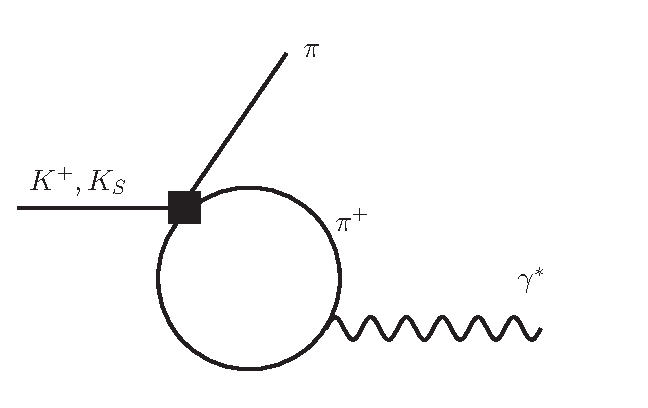
\includegraphics[scale=0.5]{figs/Cirigliano_fig17.pdf} %ks_pi0mumu.pdf}
\caption{Feynman diagram of the process \Kzpizmm. \label{fig:diagram}}
\end{center}
\end{figure}

The LHCb experiment~\cite{LHCbDet} has demonstrated very good performance in the search for rare leptonic \KS decays~\cite{Ksmm}. In this note, we evaluate the potential
sensitivity of LHCb to \BRof\Kspizmm considering the data to be collected with the LHCb detector before and after its upgrade in 2018.
 
This document is organized as follows: in~\secref{sec:strategy}, the analysis strategy is summarized; in \secref{sec:selection}, details on the signal reconstruction and selection are given;
in \secref{sec:background}, the study on the expected background sources is presented; in \secref{sec:fit}, the likelihood fit is described; in~\secref{sec:sensitivity}, the sensitivity to
\BRof\Kspizmm is reported and finally, conclusions are drawn in~\secref{sec:conclusions}.


% $Id: introduction.tex 87303 2016-02-08 13:44:29Z lafferty $

\subsection{Analysis strategy}
\label{subsec:strategy}

Decays of the \KS in LHCb are characterized by decay vertices separated from the interaction point\footnote{The \KS at LHC typically decays after traversing tens of centimeters to even several meters.}, 
and with tracks having an average transverse momentum significantly lower than those from $b$ and $c$ decays.
The transverse momentum range is similar to typical tracks generated in the proton-proton collision and hence has almost no discriminating power. 

Muon candidates are combined into $\mu^+\mu^-$ pairs. Then a $\pi^0$ can be added to the dimuon pair to make a fully reconstructed
\KS decay. However, since the reconstruction efficiency of the $\pi^0$ is limited, events in which no $\pi^0$
is found are also considered, based only on the dimuon information. This leads to two independent analyses: one for the
events in which all decay products are considered (hereafter FULL) and one in which only the dimuon pair is used
(hereafter PARTIAL). 
The reconstructed candidates are then passed through a selection algorithm followed by a {\it Boosted Decision Tree} (BDT) classification,
to reduce the high level of background.


The properties of the \Kspizmm decays are studied using simulated samples with a differential decay rate modeled according to Ref.~\cite{Gino}.
The corresponding $\mumu$ mass distribution, $m_{\mumu}$, as well as the dependence of the (cosine of the) dimuon helicity 
angle, $\cos\theta_{\mu}$ (see the angle definitions in \figref{fig:angles}), on $m_{\mumu}$ are shown in \figref{fig:EviltGen}.

 \begin{figure}[htb!]
 \begin{center}
  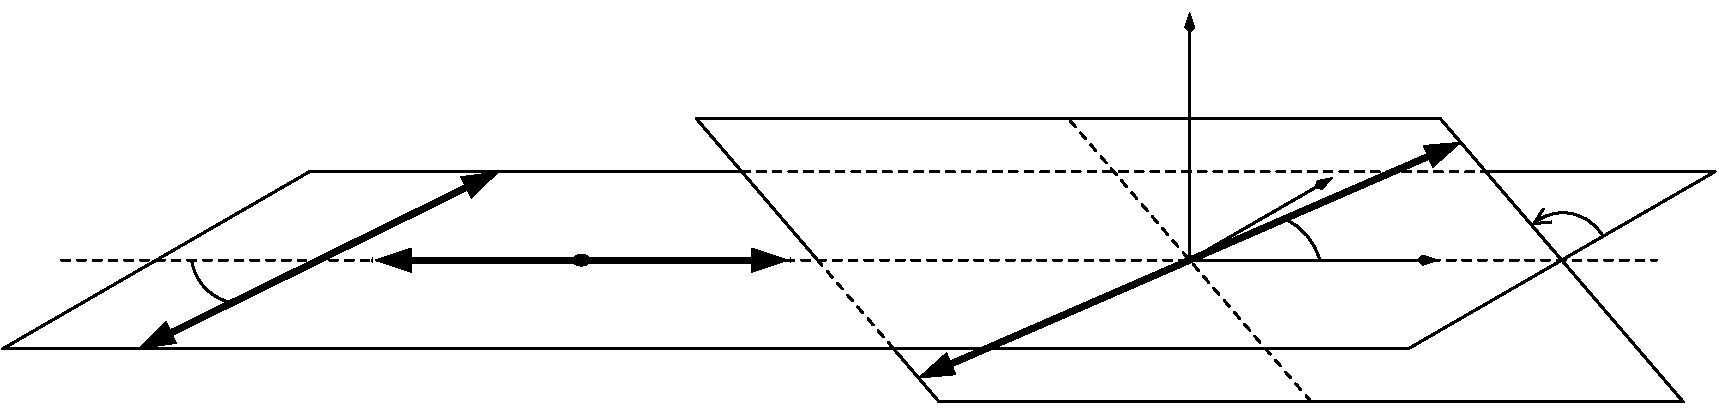
\includegraphics[scale=0.4]{figs/Kspi0MuMu/helAngles.pdf}
  \put(-27,40){${\phi_{\mu}}$}
  \put(-70,35){${\theta_{\mu}}$}
  \put(-308,21){${\phi_{\pi}}$}
  \put(-64,54){$\mu^{-}$}
  \put(-142,5){$\mu^{+}$}
  \put(-272,34){$\pi^0$}
  \put(-225,36){$\KS$}
  \put(-275,18){$\gamma$}
  \put(-250,34){$\gamma$}
  \caption{Definition of the helicity angles in the \KS\ rest frame. \label{fig:angles}}
  \end{center}

 \end{figure}

\begin{figure} [htb!]
\begin{center}
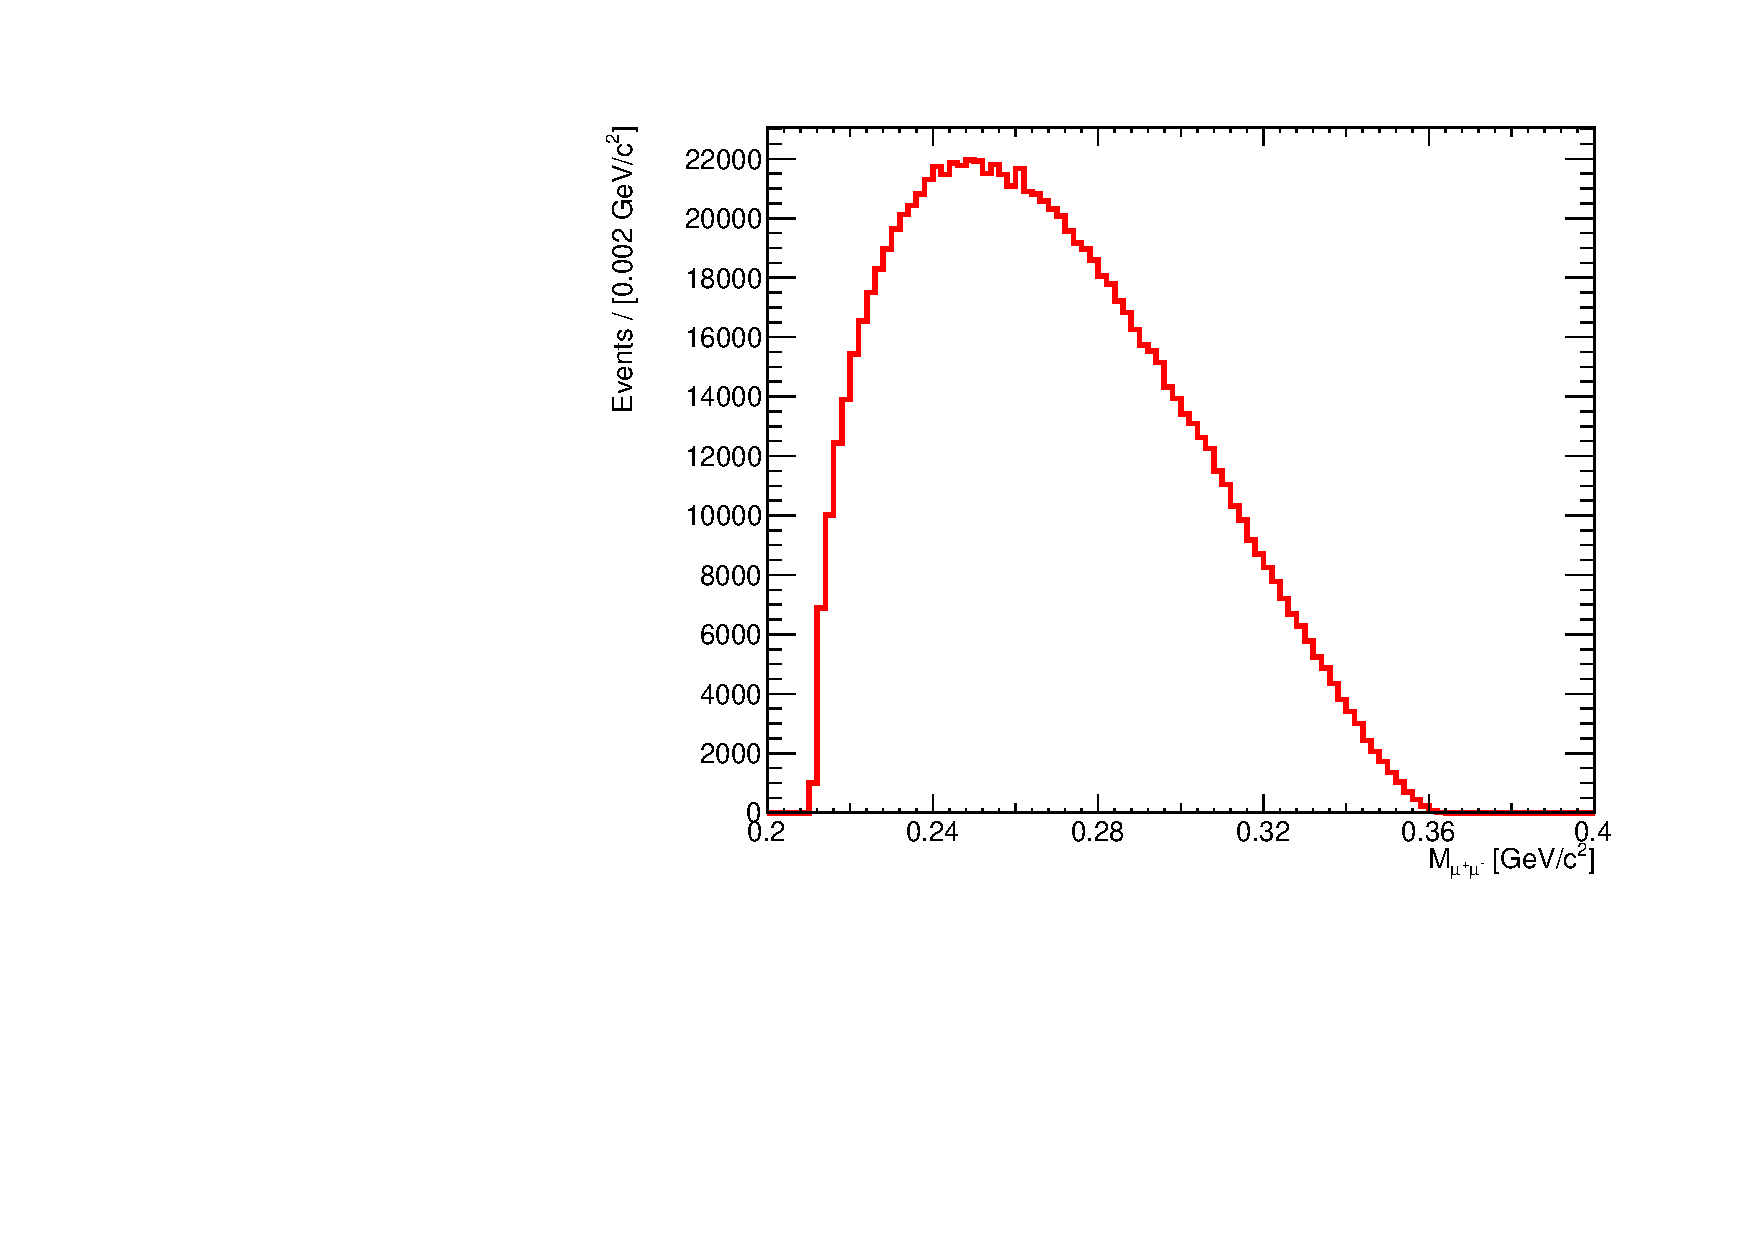
\includegraphics[scale=0.35]{figs/Kspi0MuMu/M_mumu.pdf}
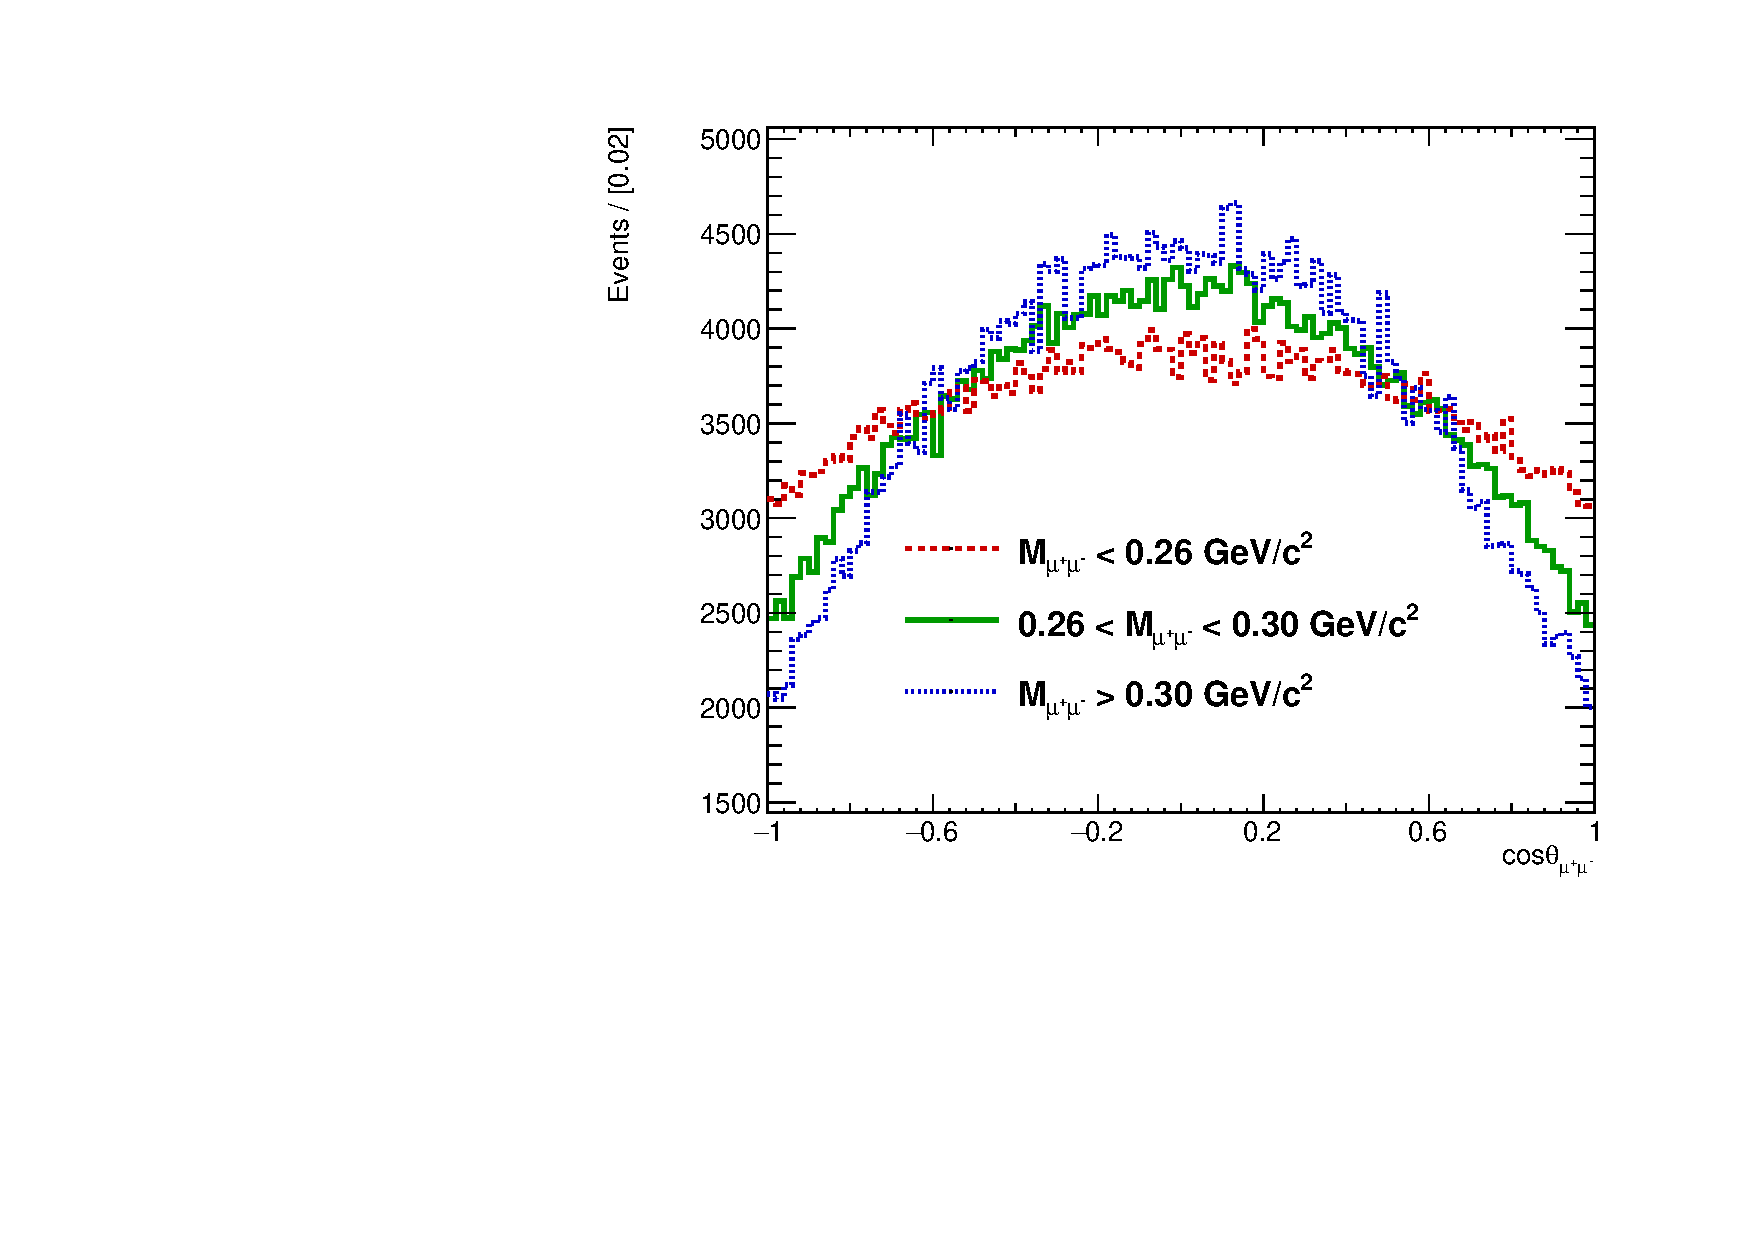
\includegraphics[scale=0.35]{figs/Kspi0MuMu/Hel_mumu.pdf}
\caption{$m_{\mu\mu}$ distribution (left), and the dimuon helicity angle depending on $m_{\mu\mu}$ (right). \label{fig:EviltGen}}
\end{center}
\end{figure}


The BDT is trained with simulated signal events and combinatorial background events from the existing LHCb data.
Since the main goal of this study is to evaluate the sensitivity for the LHCb upgrade, where the
trigger efficiency is expected to be very high, trigger unbiased data samples are preferred.
Therefore, the events are obtained from the {\it Trigger Independent of Signal} (TIS) ~\cite{TISTOS} category of the LHCb trigger. 
This means that the tracks and clusters of the reconstructed candidate are not needed to fire the trigger at any level, because
another object in the underlying event already fired it.
This ensures an almost trigger unbiased data set, while still providing a sample much larger than random selection triggers. 

%The expected signal yield is obtained assuming the NA48 central value for \BRof\Kspizmm, the observed \Kspipi yield from data and
%the efficiency ratio \textcolor{red}{$\frac{\epsilon_{\KsPzMuMu}}{\epsilon_{\PKzS\to\Pgpp\Pgpm}}$} obtained in simulation (See \eqref{eq:normalization}). 

The expected signal yield is obtained assuming the NA48 central value for \BRof\Kspizmm, normalizing the signal yield with respect to \Kspipi as 
\begin{equation}
      \frac{N(\KsPzMuMu)}{N(\PKzS\to\Pgpp\Pgpm)} = 
      \frac{{\cal B}(\KsPzMuMu){\epsilon_{\KsPzMuMu}}}
      {{\cal B}(\PKzS\to\Pgpp\Pgpm){\epsilon_{\PKzS\to\Pgpp\Pgpm}}},
\label{eq:normalization}
\end{equation}
where the observed \Kspipi yield is extracted from data and the efficiency ratio, $\frac{\epsilon_{\KsPzMuMu}}{\epsilon_{\PKzS\to\Pgpp\Pgpm}}$, is obtained from simulation.

The \BRof\Kspizmm sensitivity is measured in a pseudo-experiment study. First, the signal and background yields are extrapolated
for a desired expected luminosity and trigger efficiency, then pseudo-experiments are generated according to those yields. 
The \BRof\Kspizmm uncertainty is obtained from a fit to the \KS mass distribution of the pseudo-experiments, using the signal and background
models obtained from MC and the fit to the available LHCb data, respectively. The mass fit range is $[420,580] \mevcc$.
 




% $Id: introduction.tex 87303 2016-02-08 13:44:29Z lafferty $

\subsection{Reconstruction and selection}
\label{subsec:selection}

Pairs of muon candidates are reconstructed combining opposite-charged tracks with hits in the vertex locator (VELO), trigger tracker, tracker stations, and muon chambers. 
In addition, the tracks are required to be separated by at least $6\sigma$ from any $p-p$ collision point in the event.
Tracks with transverse momentum lower than 80\mevc are ignored. 
A dimuon candidate pair can be combined with a $\pi^0$ candidate to build a \KS\ candidate. 
The events in which the entire decay chain is used are classified as FULL. When only the dimuon information is used, they are clasified as PARTIAL.

Neutral pion candidates are reconstructed from 
$\gamma$ candidate pairs that correspond to two independent clusters in the calorimeter.
Each photon candidate is required to have a transverse momentum of
at least 200\mevc and the pion candidate a mass within 30\mevcc of the world average $\pi^0$ mass.
The mass resolution is then improved by constraining the $\pi^0$ candidate 
mass to the world average $\pi^0$ mass, and by constraining the three-momentum
vector of the \KS to point back to the production vertex. For the PARTIAL candidates, a momentum vector with an absolute value of $\approx 10\gevc$
is used as a representative of the $\pi^0$ momentum when calculating the invariant mass. As a consequence of these kinematic constraints, the \KS\ candidate 
mass resolution depends only weakly on the $\pi^{0}$ momentum.

Additional selection requirements are applied to reduce the
amount of data to analyze, fulfil the rate requirements for LHCb offline
processing and reduce the amount of background. These include a \KS\ candidate lifetime of at least $1\;\rm ps$
and removing events in the kinematic region of $\Lambda\to p \pi$ and $\KS\to \pi^{+}\pi^{-}$ in the Armenteros-Podolanski plane~\cite{Armenteros}.
The total reconstruction and selection efficiency for the FULL channel is $5.47\times10^{-4}$.

Requiring a well-reconstructed  $\pi^0$ implies an inefficiency penalty of a factor ten.
Thus, a complementary strategy for the PARTIAL candidates is also investigated.
Indeed, the constraints on the $\pi^0$ mass and the \KS momentum are sufficient to create a peaking distribution if there is an estimate of the typical
value of the $\pi^0$ momentum ($\approx 10\gevc$), as shown in \figref{fig:peaks}.
A comparison of the reconstructed mass resolution between FULL and PARTIAL is difficult due to the asymmetric and non-Gaussian distribution of the PARTIAL case. To get an estimate, the corresponding 
FWHM values are calculated. In the FULL case, it is 23.3~\mevcc and in the PARTIAL 40.6~\mevcc.

The PARTIAL selection does not require any information about a reconstructed $\pi^0$. Some
requirements had to be tightened in order to keep the background at a manageable level. These include a lower distance of closest approach between the two
muon tracks; a minimum requirement on the \KS\ vertex quality, $\chi^{2}/ndof = 9$; a higher minimum requirement on the \KS\ vertex detachment from the interaction point;
and minimum radial, $z$- and absolute distance requirements between the \KS\ vertex and the interaction point.
The total reconstruction and selection efficiency for the PARTIAL analysis is $3.0\times 10^{-3}$ , well above that of the FULL,
but at a cost of an increased background yield.

\begin{figure} [htb!]
\begin{center}
%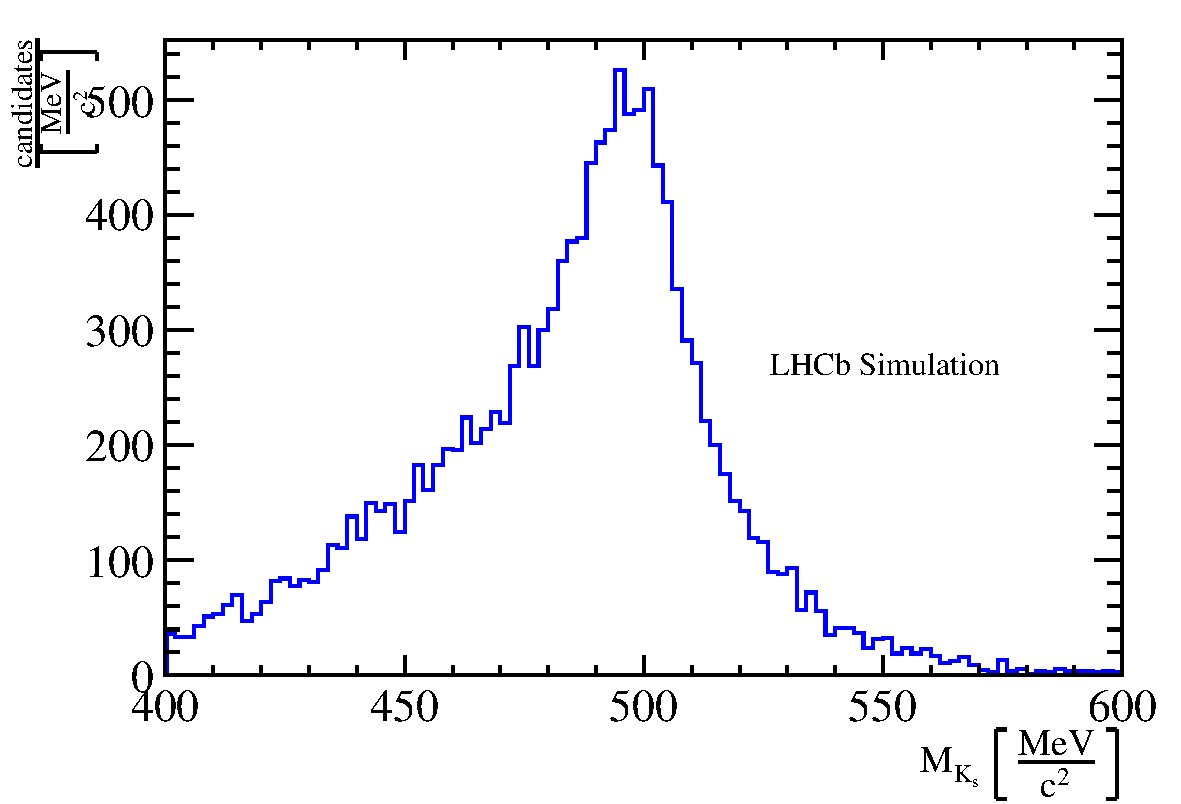
\includegraphics[scale=0.35]{figs/hphantom.pdf}
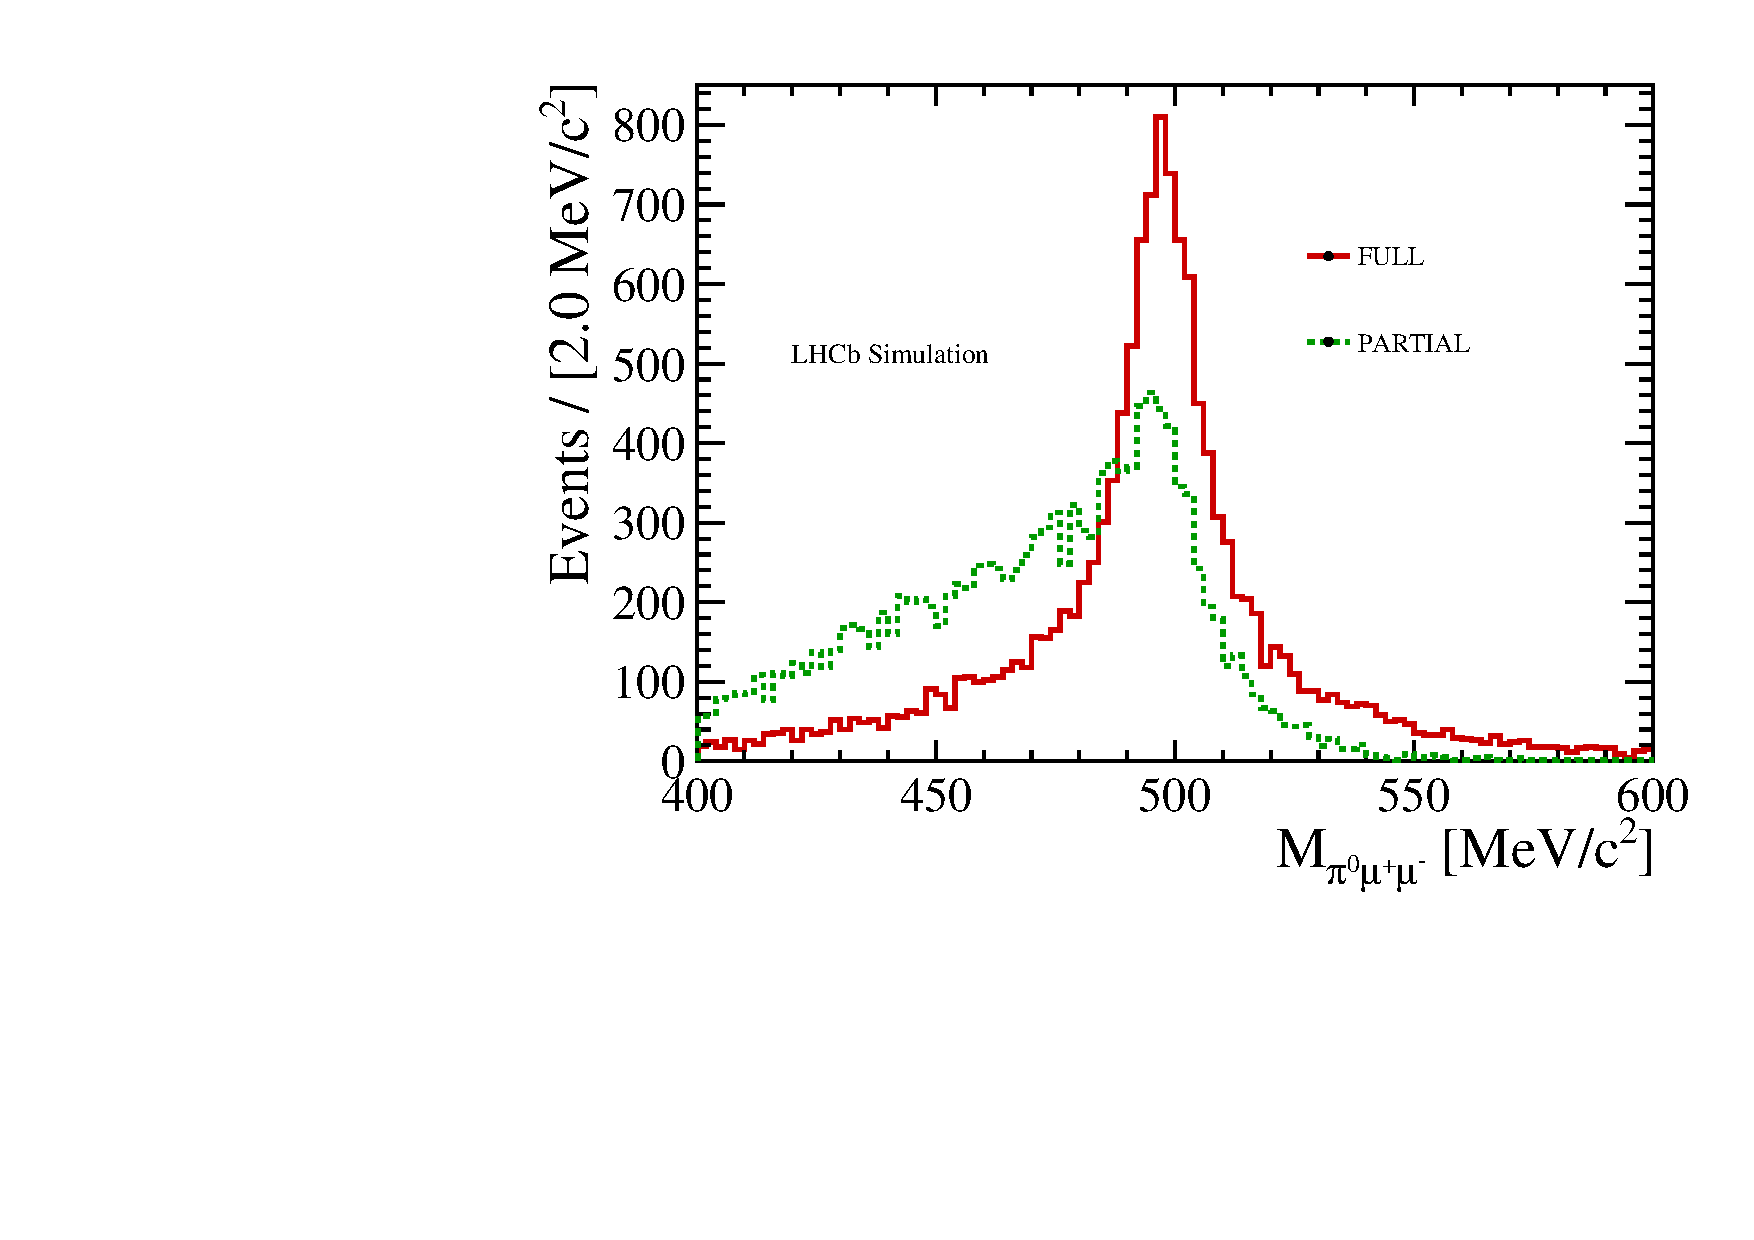
\includegraphics[scale=0.6]{figs/Kspi0MuMu/M_V0_vs_VC.pdf}
\caption{Comparison between the FULL (solid red) and PARTIAL (dashed green) kaon candidate mass distributions. \label{fig:peaks}}
\end{center}
\end{figure}

A BDT is used to separate signal from combinatorial background. It is trained with MC events (signal class) and a part of the data that is not used in the fit
(combinatorial background class). The BDT uses information about the geometrical properties of the events,
kinematics, track quality, and muon identification quality. The BDT response for signal and background for both FULL and PARTIAL 
is shown in \figref{fig:BDT}.


\begin{figure} [htb!]
\begin{center}
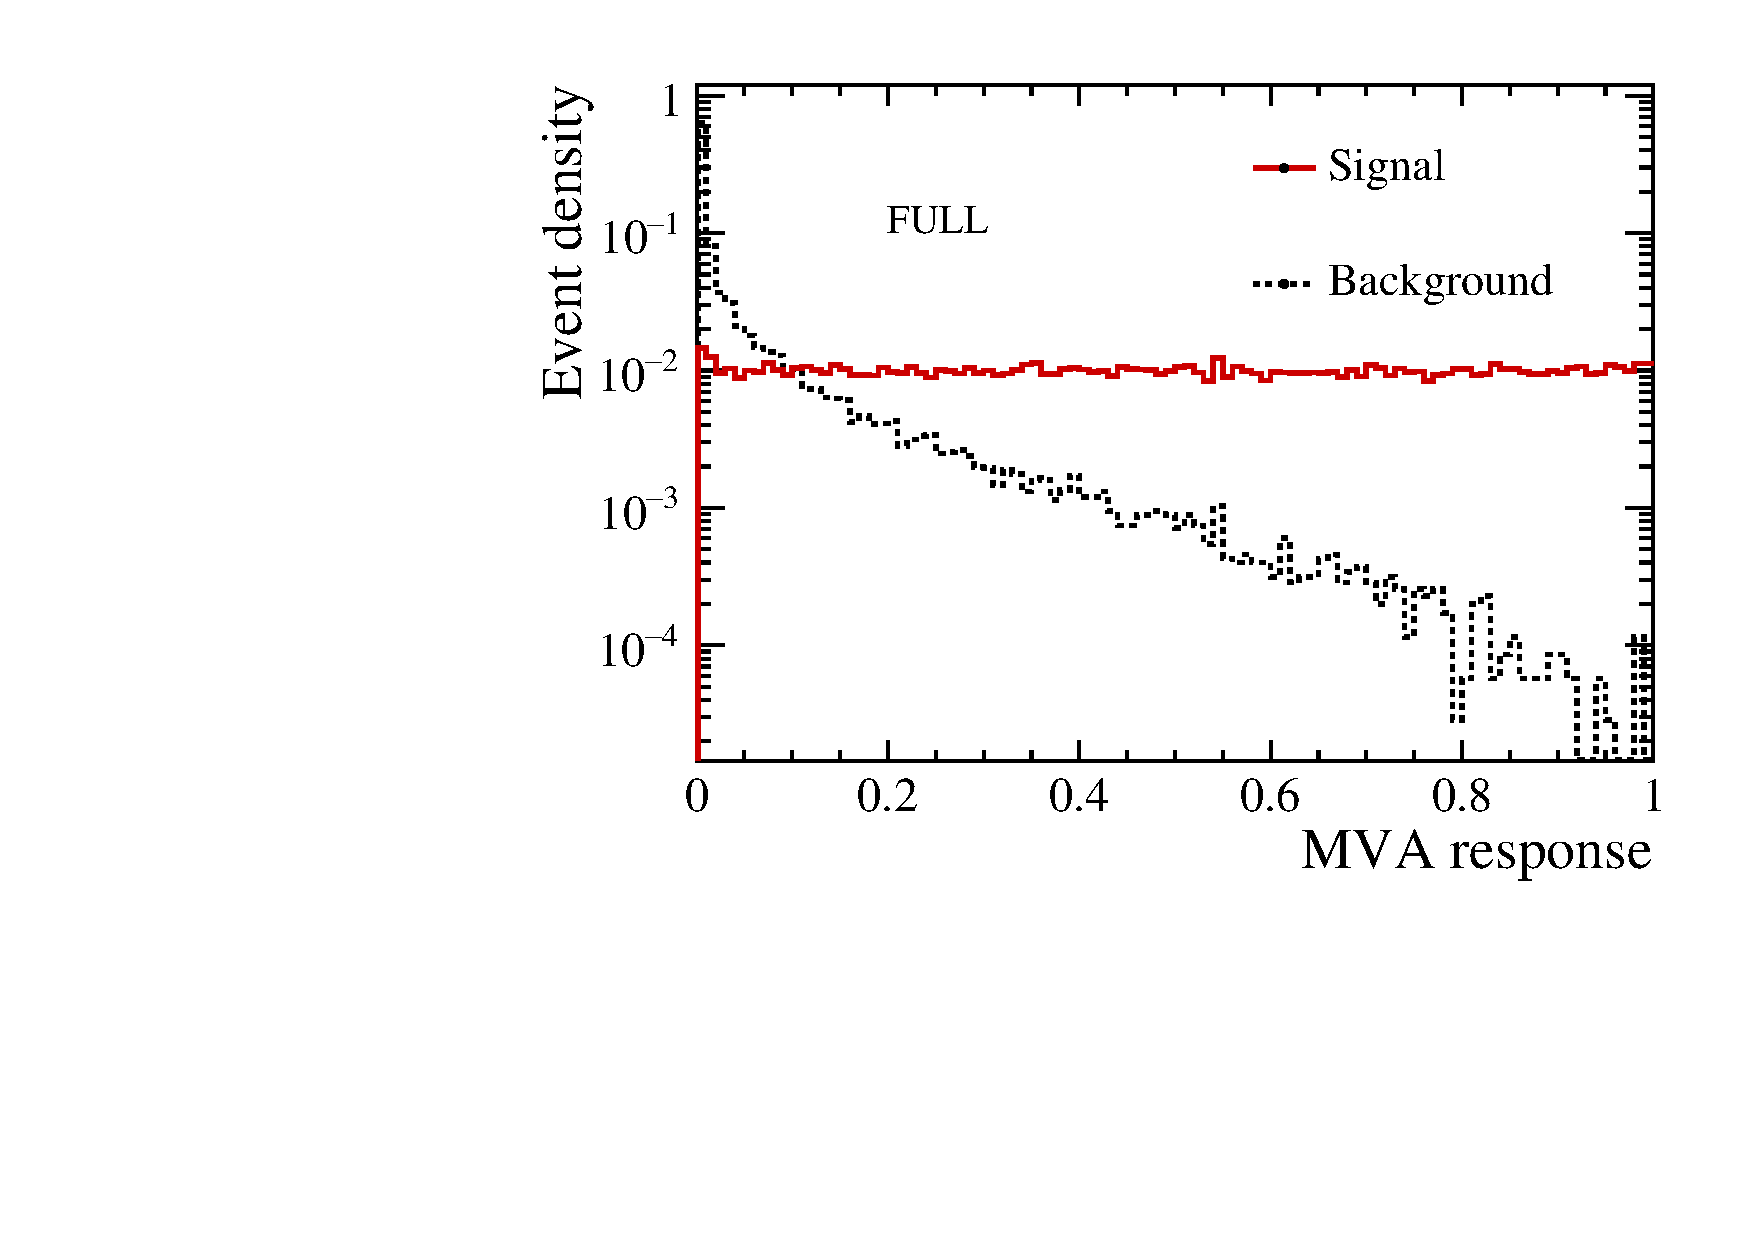
\includegraphics[scale=0.38]{figs/Kspi0MuMu/BDT_sig_vs_bkg_FULL.pdf}%BDTFULL.pdf}
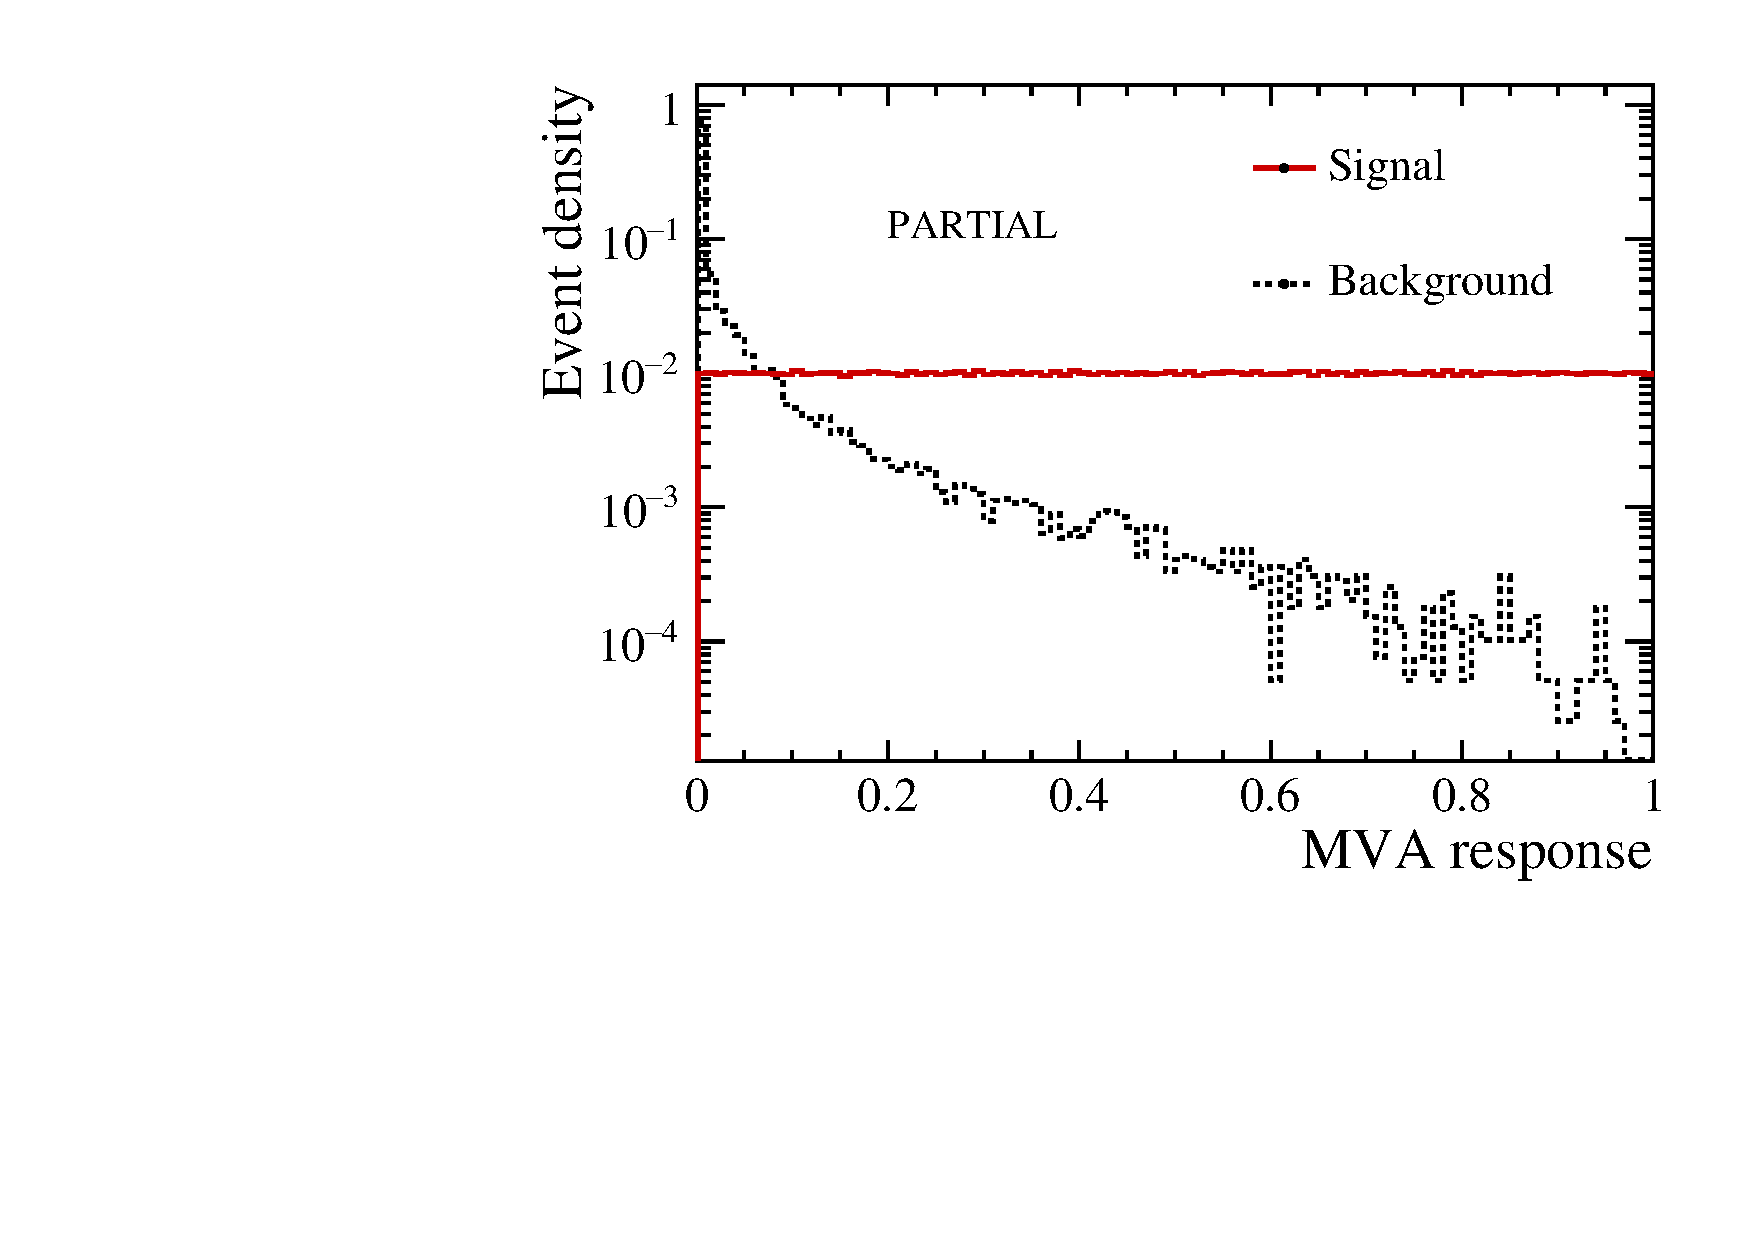
\includegraphics[scale=0.38]{figs/Kspi0MuMu/BDT_sig_vs_bkg_PARTIAL.pdf}%BDTPARTIAL.pdf}
\caption{BDT response both for signal (solid red) and background (dashed black). Right: FULL channel. Left: PARTIAL channel.  Signal and background are normalized to the same area. \label{fig:BDT}}
\end{center}
\end{figure}


The events are classified in four bins of the BDT response. The signal yields are obtained in a simultaneous fit 
of the mass distribution in each BDT bin, as described in the following sections.


% $Id: introduction.tex 87303 2016-02-08 13:44:29Z lafferty $

\subsection{Background sources}
\label{subsec:background}

Several sources of background are investigated to assess their relevance for a measurement of \BRof\Kspizmm:
\begin{itemize}
%\item Misidentified \Kspipi decays (combined with a combinatorial $\pi^0$ in the case of FULL). 
\item \Kspipi decays, where both pions are misidentified as muons, and in the case of the FULL category, combined with a random $\pi^0$ from the underlying event.
These decays have a mass larger than that of the \KS and do not enter the fit region, except for potential residual tails that effectively add up to the combinatorial background. % TODO (see \figref{fig:Kspipibkg}). 
No evidence for \Kspipi background is seen for the BDT region being fitted. 
\item \KTmTg decays. This background was considered in the NA48 analysis ~\cite{NA48}, 
However, its contribution at LHCb is found to be negligible: In the case of the \KL decay (with a branching fraction of $1.0^{+0.8}_{-0.6}\times10^{-8}$ ~\cite{PDG}) the upper decay time acceptance introduces 
an effective $10^{-3}$ reduction with respect to \KS and hence
the effective \BRof\KLTmTg becomes as low as $10^{-11}$. There is no experimental measurement of \BRof\KSTmTg, however, since
the process is dominated by the two-photon exchange\footnote{Isidori and D'Ambrosio, private communication.}, it can be estimated as:
\begin{equation}
\BRof\KSTmTg = \frac{\BRof\KSTg}{\BRof\KLTg}\BRof\KLTmTg \sim 4.8\times10^{-11}
\end{equation} 
\noindent and is thus negligible.
\item \KLTpi decays. The mass distribution of these decays is shown in \figref{fig:KLTpi} as obtained in simulation. Since there is no evidence of this background in the 
data, it is neglected. Including a \KLTpi component to the observed background does not change significantly the sensitivity estimates. The \KS counterpart has a branching fraction of $3.5\times10^{-7}$ and thus
is about four orders of magnitude smaller than \KLTpi. In general, no sign of a resonant structure in the $\pi^+\pi^-\pi^0$ is seen on data.

\item Combinatorial background. Combinatorial background is considered to be composed by random combination of tracks, including those generated by pseudo-random combinations of hits during the pattern recognition. 
It has a monotonic shape across the studied invariant mass range.

\end{itemize}

\begin{figure} [htb!]
\begin{center}
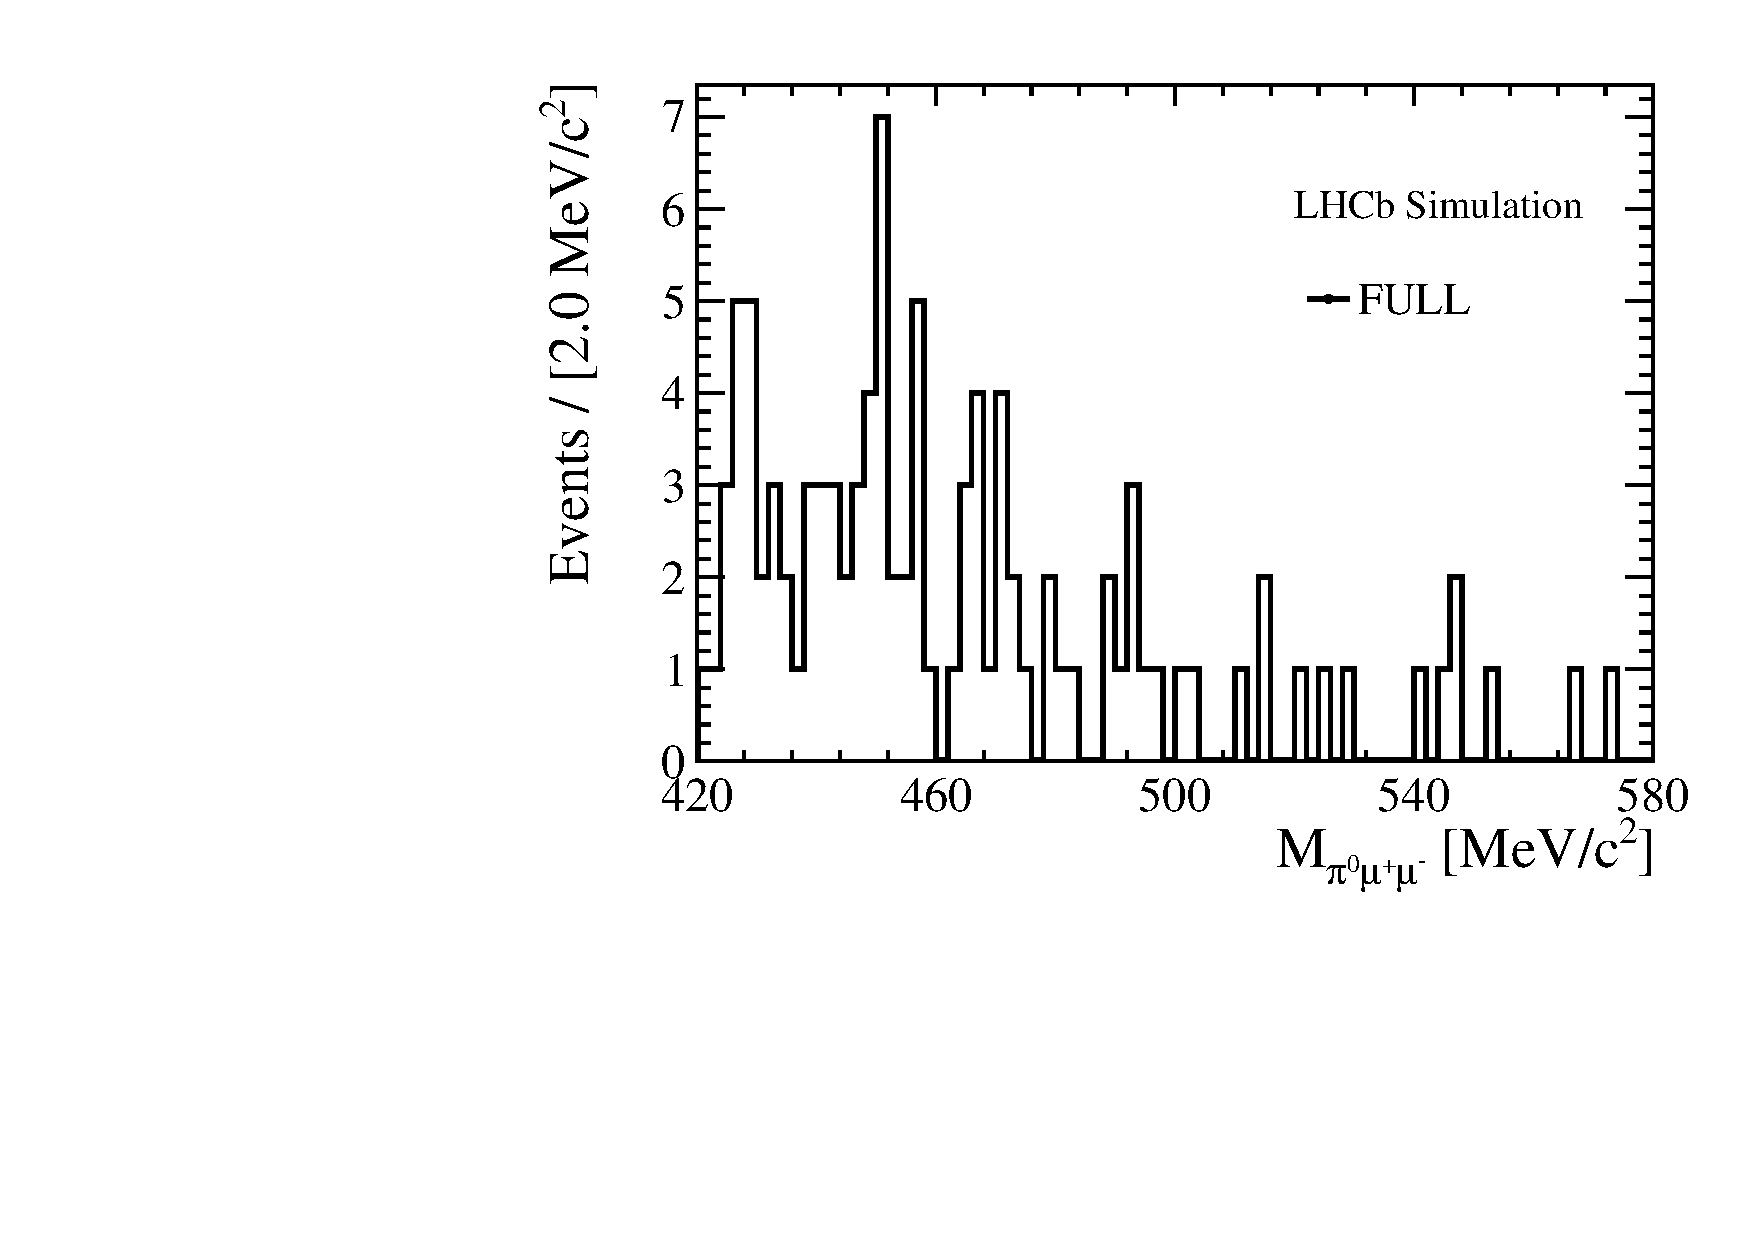
\includegraphics[scale=0.30]{figs/Kspi0MuMu/M_VC_K3pi.pdf}%{figs/K3pi_FULL.pdf}
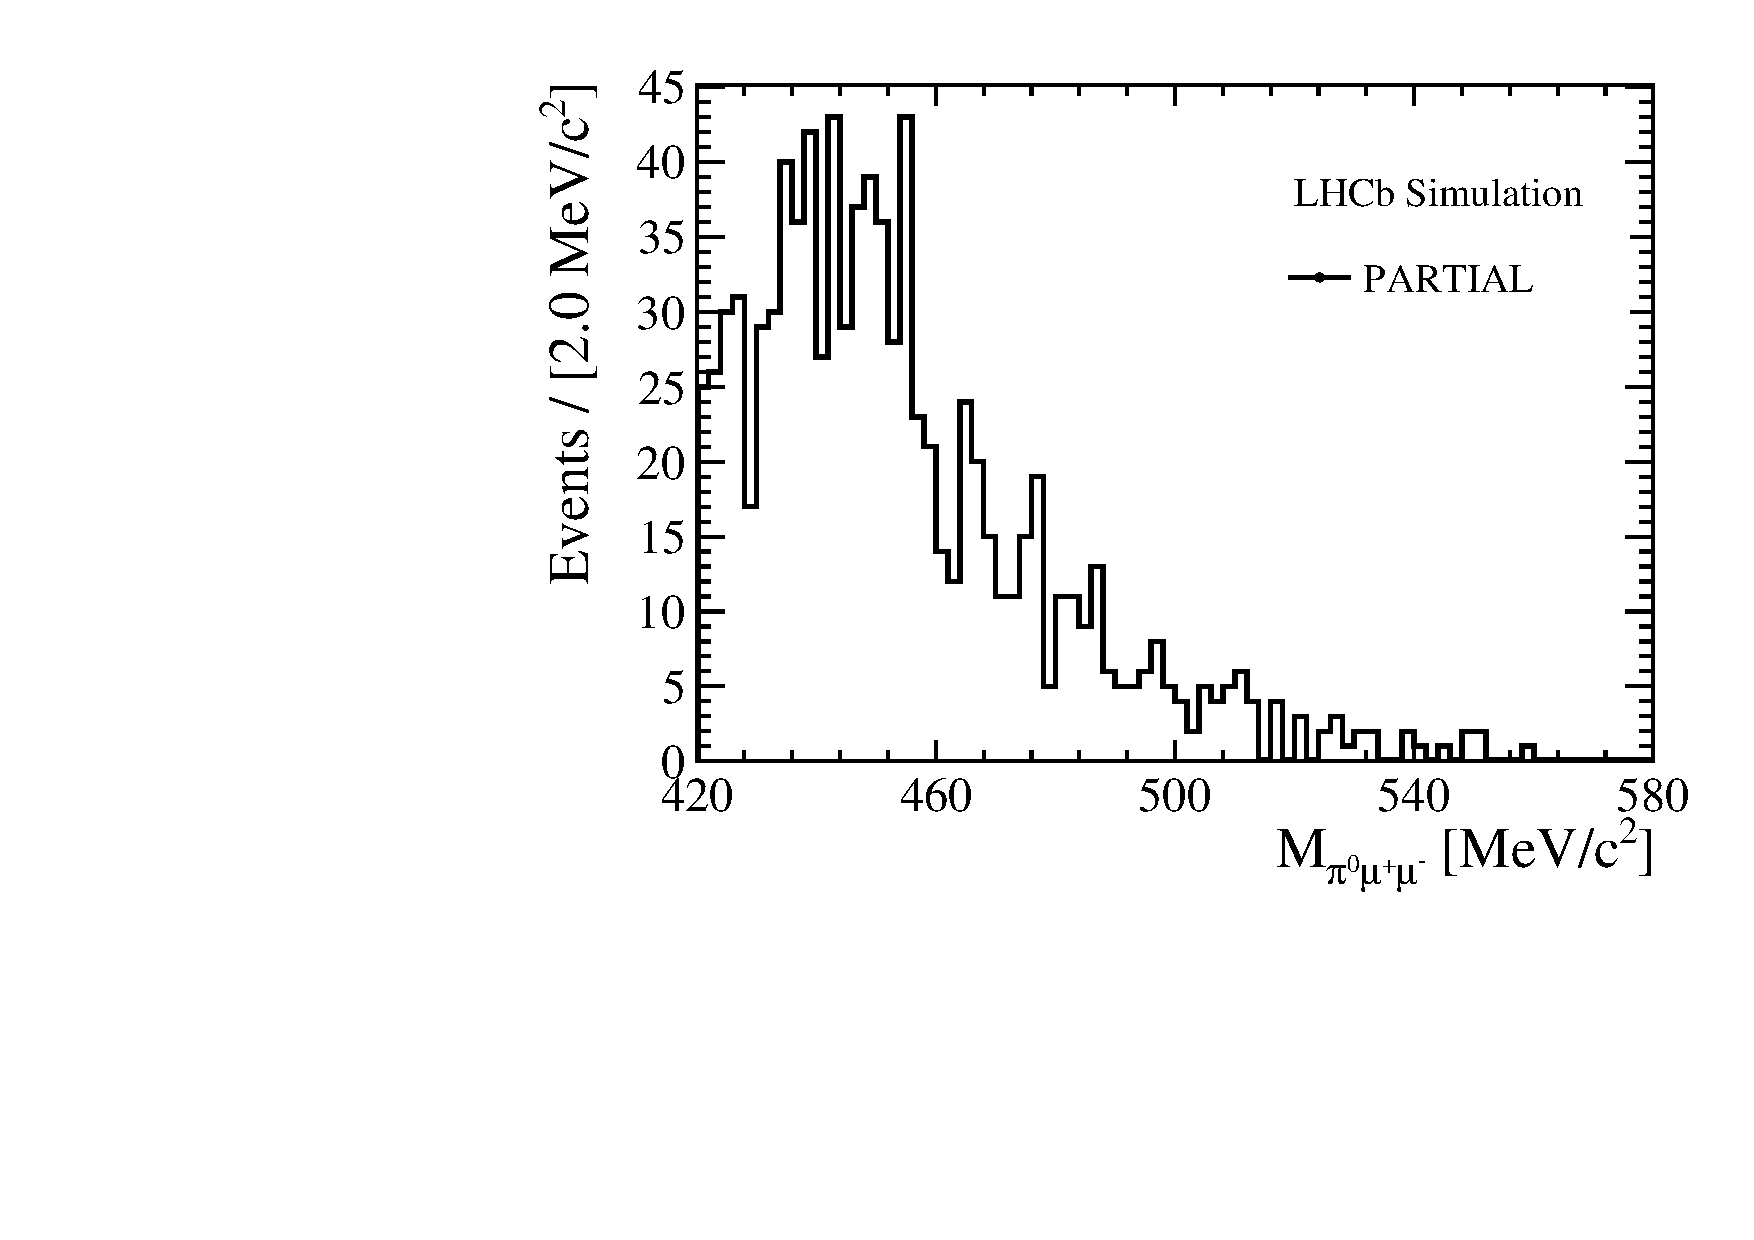
\includegraphics[scale=0.30]{figs/Kspi0MuMu/M_V0_K3pi.pdf}%{figs/mK3pi_PARTIALL.pdf}
\caption{Invariant mass distribution of simulated $K^0\rightarrow\pi^+\pi^-\pi^0$ decays selected in the FULL (left) and PARTIAL (right) categories.  \label{fig:KLTpi}}
\end{center}
\end{figure}



% $Id: introduction.tex 87303 2016-02-08 13:44:29Z lafferty $

\subsection{Fit model}
\label{subsec:fit}
Only events in the BDT range [0.6,1] are considered in the fit to the data.
A simultaneous fit to the mass distribution across four equally-sized
independent bins of the BDT response is performed. The combinatorial background is described
with an exponential \pdf for both FULL and PARTIAL analysis, with independent floating yields and
decay constants in each BDT bin. The signal
model is an Hypathia distribution~\cite{Ipatia} with different configurations
for FULL and PARTIAL (see \figref{fig:Ipatia}). The signal model parameters are independent
in each BDT bin and are obtained from simulation. The fractions of signal events allotted to each
BDT bin are also fixed from values obtained from simulation, with a total signal yield remaining as the sole free parameter describing signal in the simultaneous fit. %%%\textcolor{red}{J: What do you do with the background?}
The signal yield is floated in the fit to the data. It is measured to be 
compatible with zero within one to two sigma. %, given the limited size of the data sample.
The fit projections to the FULL and PARTIAL data are shown in \figref{fig:fit}.% and \figref{fig:fitPARTIAL},respectively.
\begin{figure} [htb!]
\begin{center}
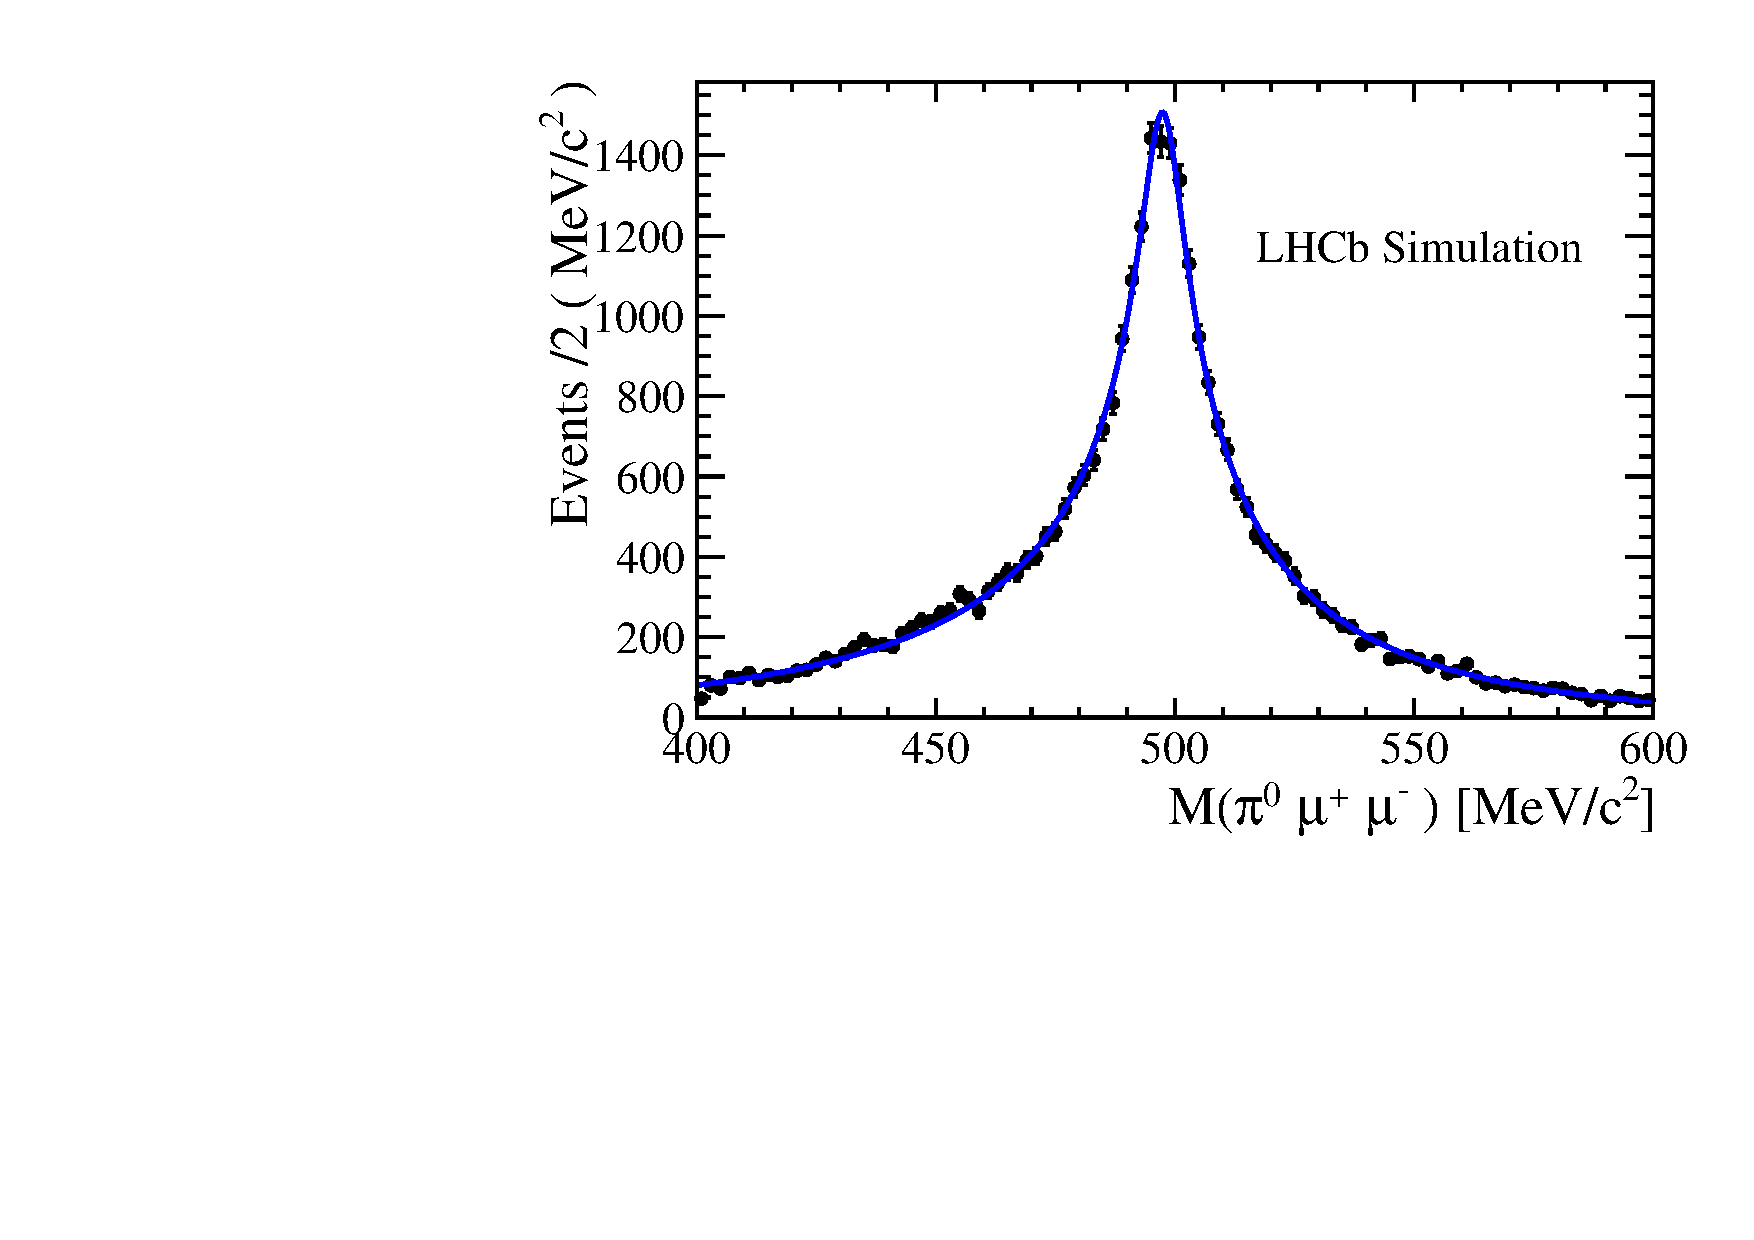
\includegraphics[scale=0.30]{figs/Kspi0MuMu/Ipatia_pi0.pdf}
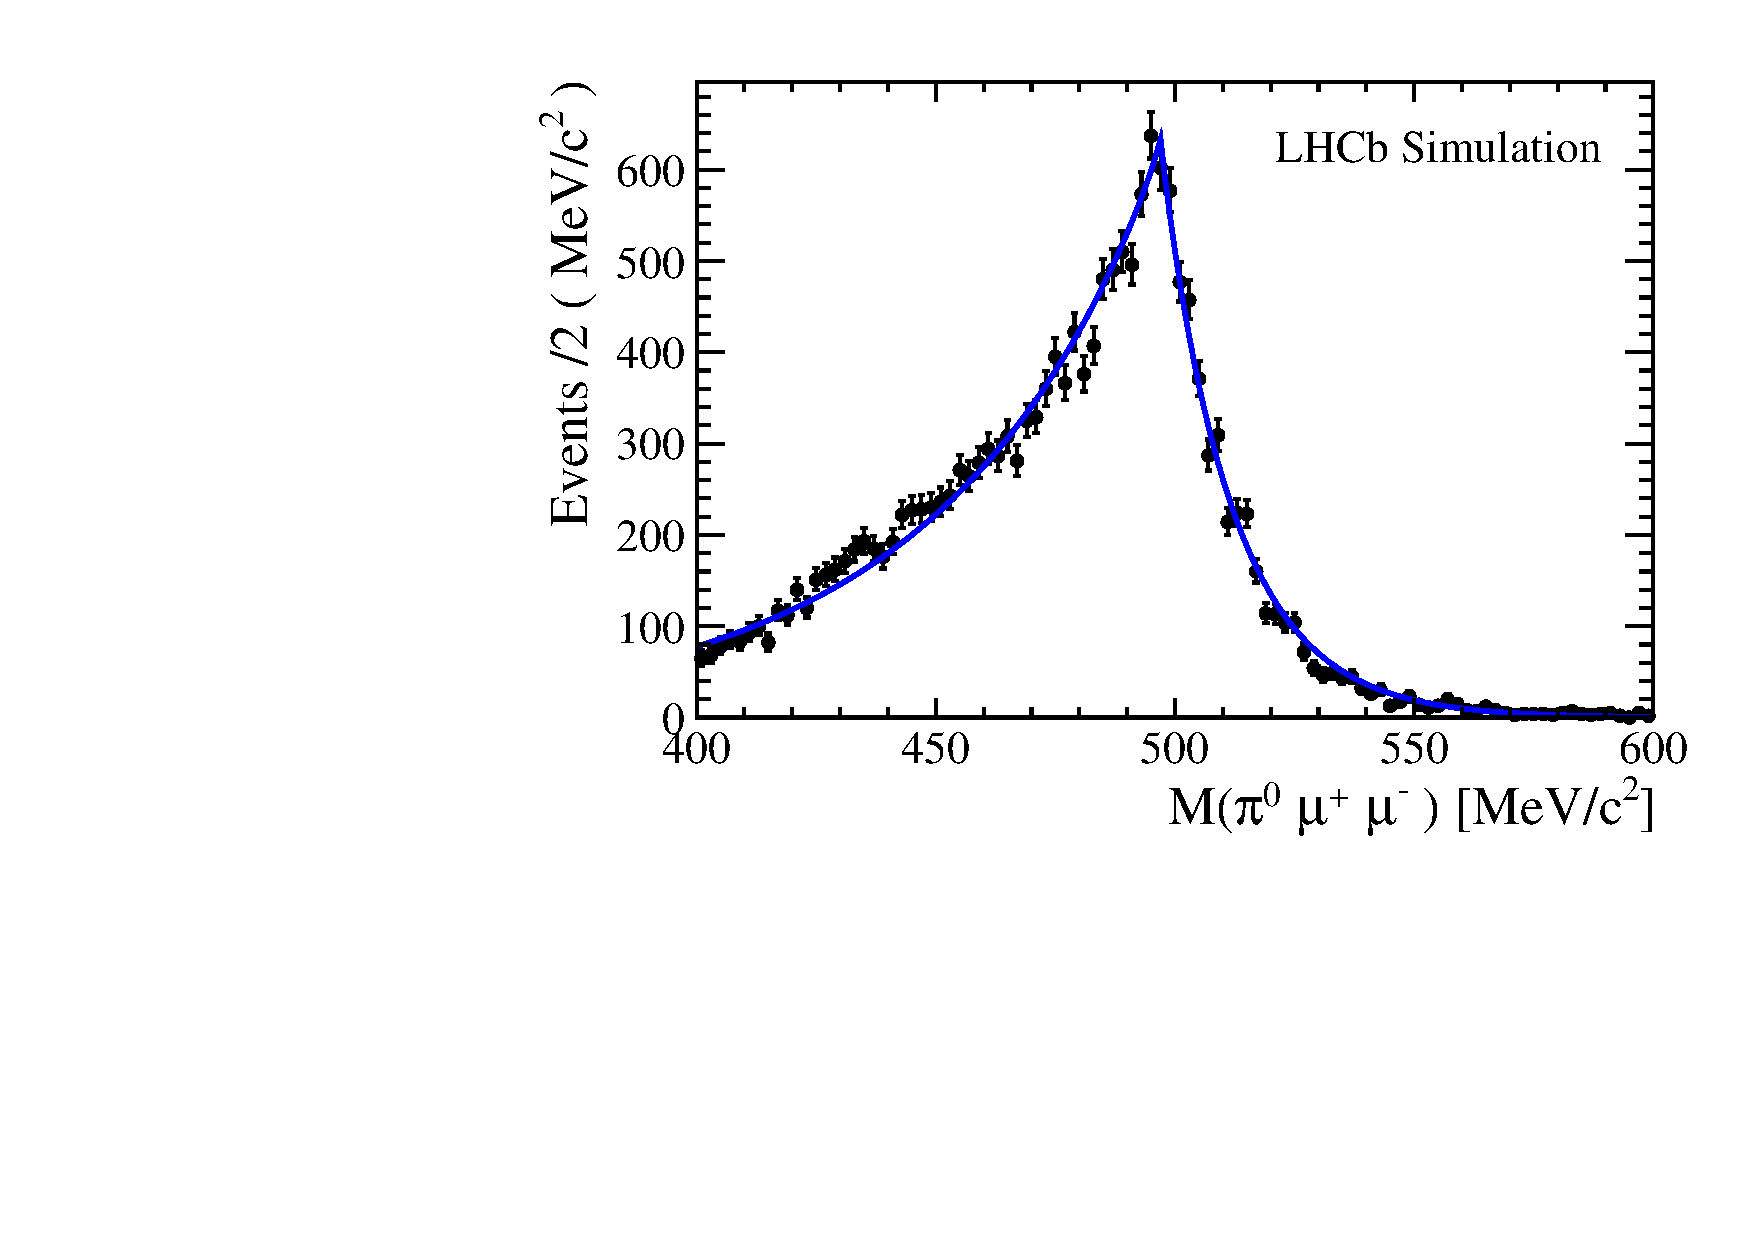
\includegraphics[scale=0.30]{figs/Kspi0MuMu/Ipatia_nopi0.pdf}
\caption{Signal fit using the Hypathia function for FULL (left) and PARTIAL (right) categories. \label{fig:Ipatia}}
\end{center}
\end{figure}

\begin{figure} [htb!]
\begin{center}
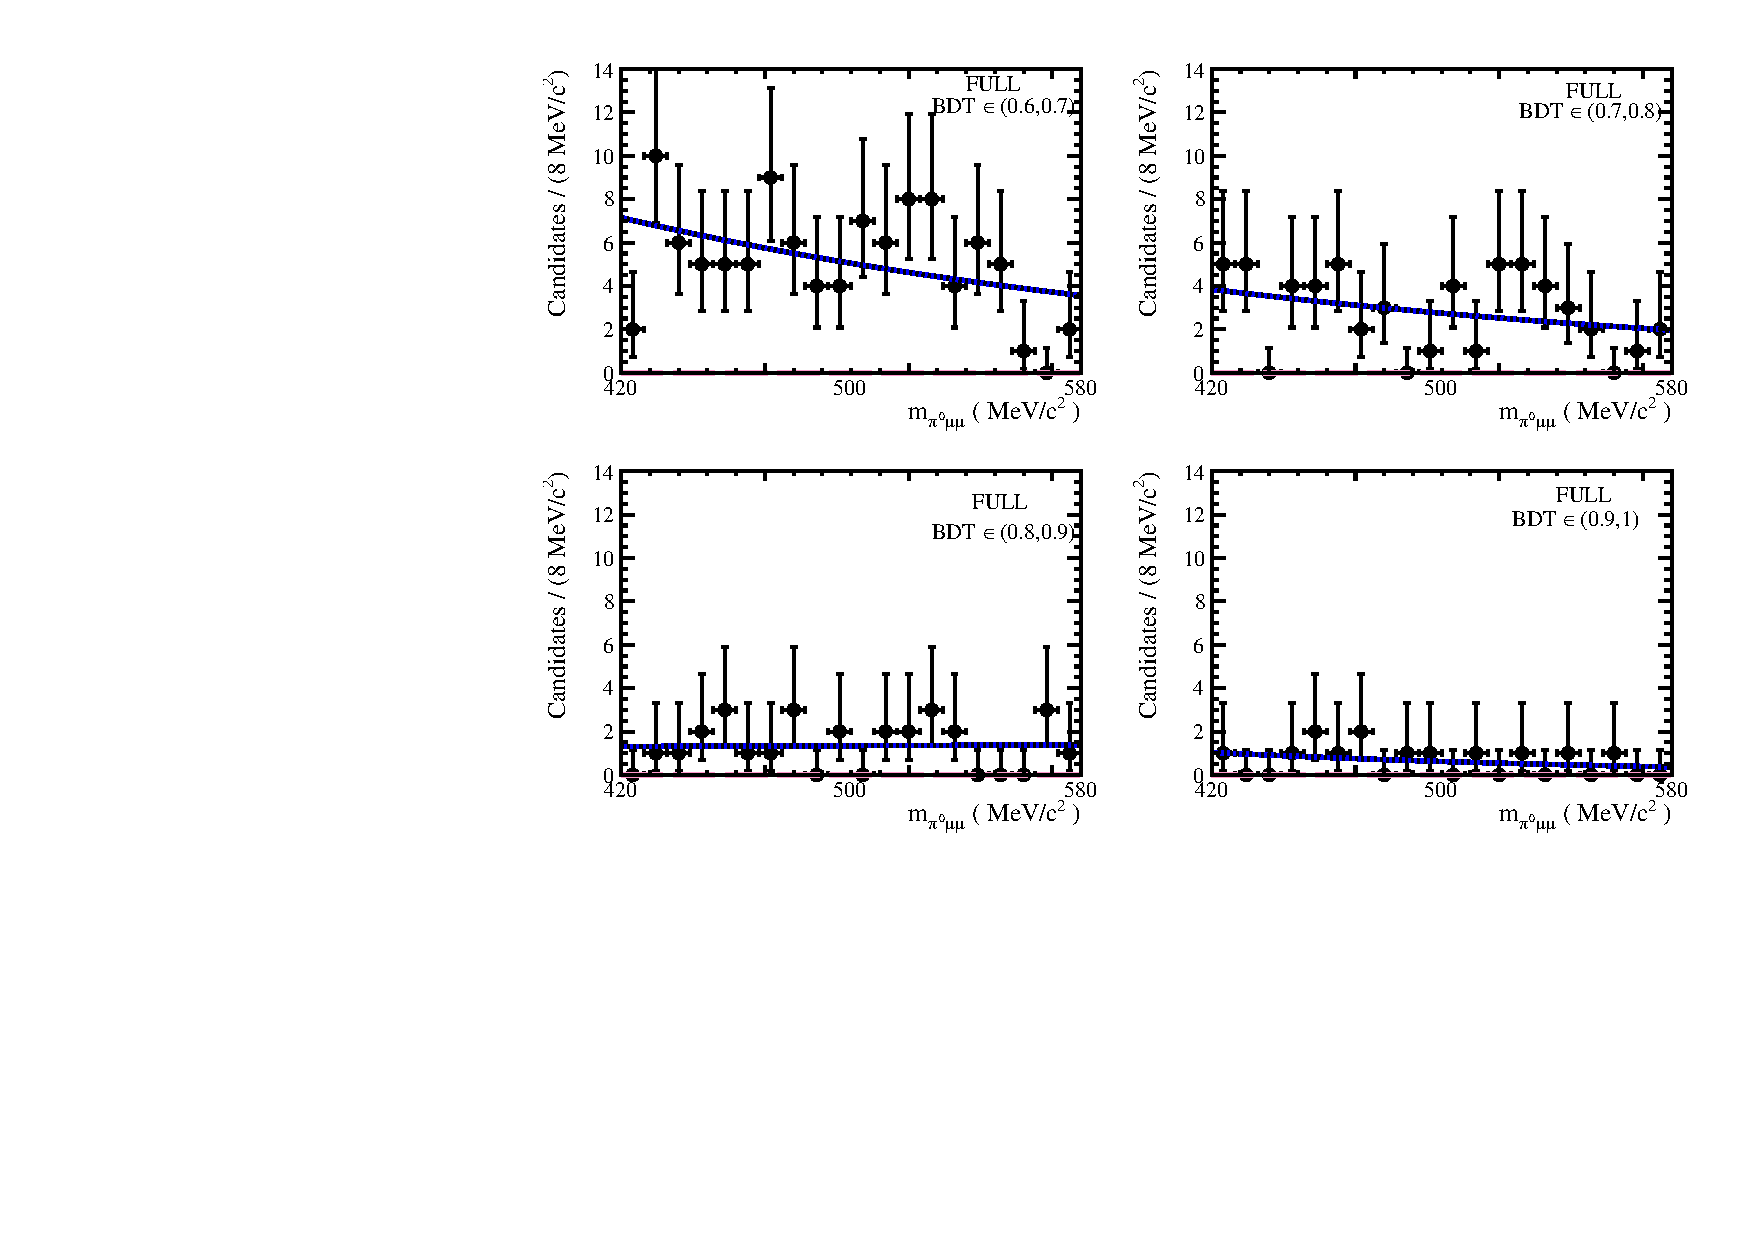
\includegraphics[scale=0.60]{figs/Kspi0MuMu/fit_FULL.pdf}
%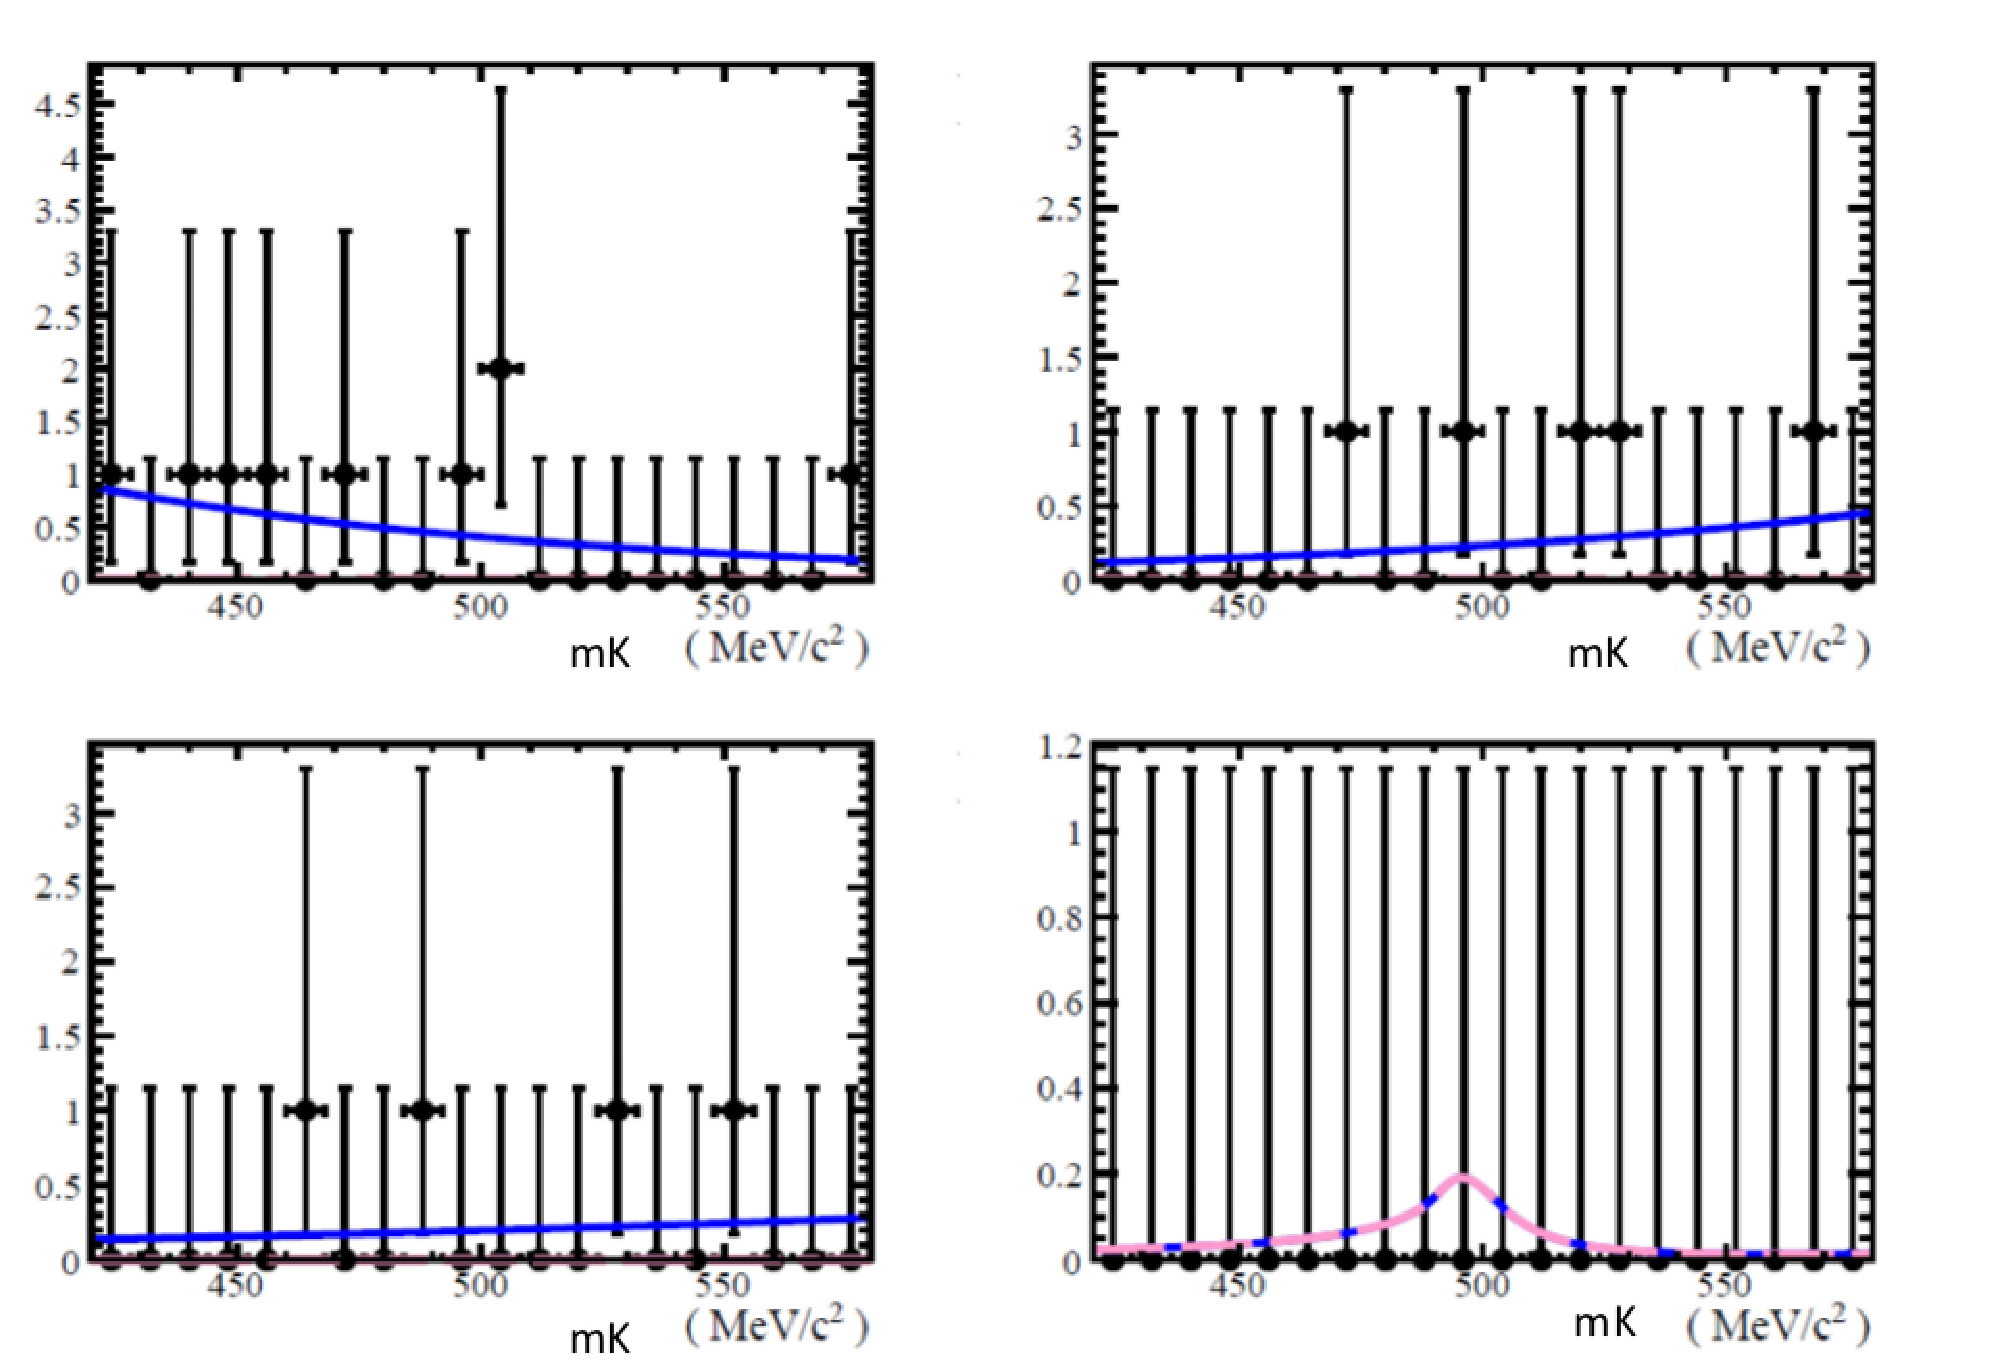
\includegraphics[scale=0.20]{figs/fit_15.pdf}
\includegraphics[scale=0.60]{figs/Kspi0MuMu/fit_PARTIAL.pdf}

\caption{Fit to data for FULL (top) and PARTIAL (bottom) categories. The magenta dashed line shows the signal contribution, the dotted black line the background, and the solid blue line the prediction from the total fit
model.
\label{fig:fit}}
\end{center}

\end{figure}

%\begin{figure} [htb!]
%\begin{center}
%%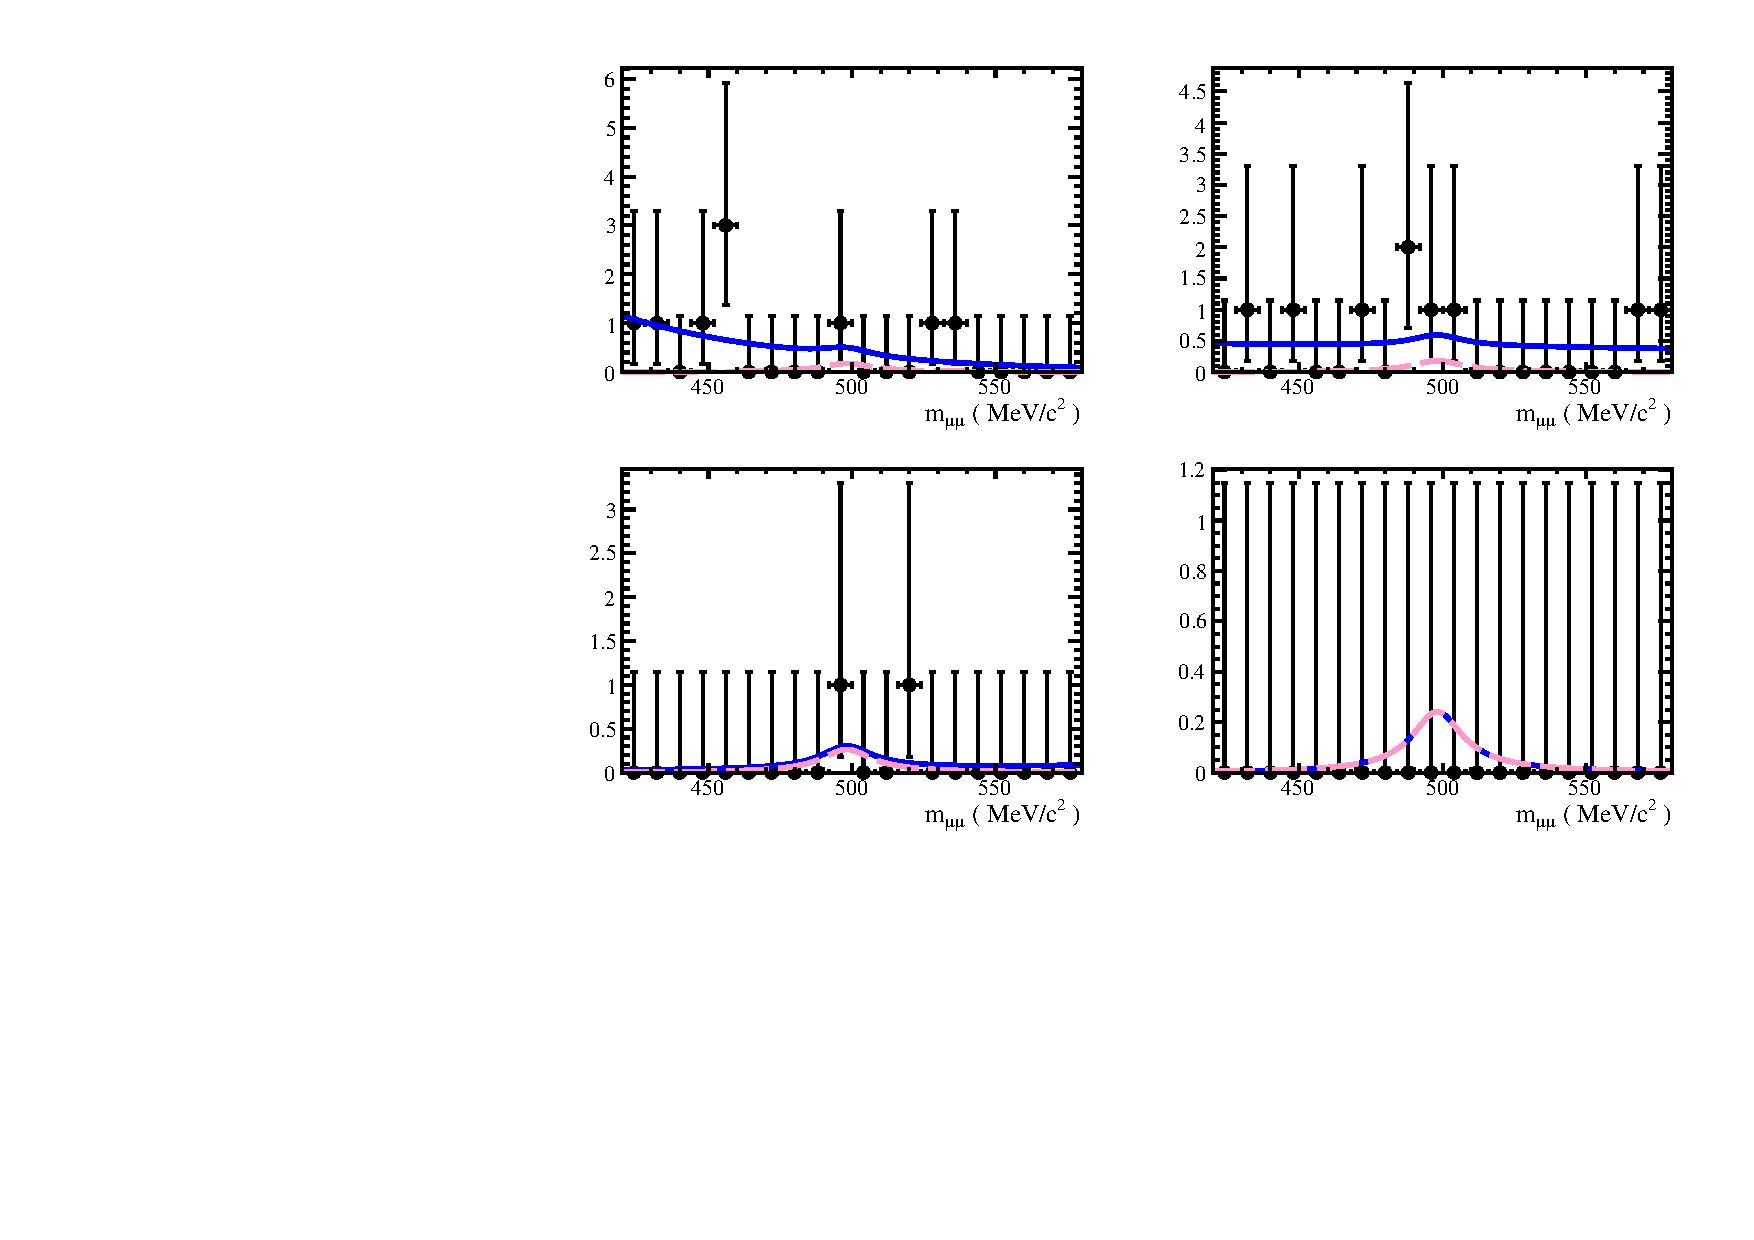
\includegraphics[scale=0.60]{figs/fit_kpmm.pdf}
%\includegraphics[scale=0.60]{figs/fit_PARTIAL.pdf}
%\caption{Fit to data for PARTIAL category. \label{fig:fitPARTIAL}}
%\end{center}
%\end{figure}


%\begin{itemize}
%\item For FULL, we find that the peak shape can be effectively described considering only the 
%resolution parameters
%\end{itemize}


% $Id: introduction.tex 87303 2016-02-08 13:44:29Z lafferty $
\subsection{Expected sensitivity}
\label{subsec:sensitivity}

The expected statistical precision on \BRof\Kspizmm for multiple values of the integrated luminosity up to 100 \invfb is estimated in this section.
% The fit to the available data performed in \secref{sec:fit} allows obtaining the model parameters of the background. 
The TIS samples used are equivalent to a 100\% trigger efficiency sample with an integrated luminosity of 4.9 and 0.77 \invpb for the FULL  and PARTIAL samples, respectively. %This effective luminosity, $L_{eff}^{dat}$, 
%has been estimated using the \Kspipi decays present in the sample, as well as the \Kspipi TIS efficiency, which is $\approx2\times10^{-3}$ as measured using the TISTOS method~\cite{TISTOS}.
The expected background yield is extrapolated from the current data fit result, where the signal yield is consitent with zero.
The background yield is scaled linearly for larger integrated luminosities.
%\begin{equation}
%N_{bkg}^L = N_{bkg}^{dat}\times\frac{L}{L_{eff}^{dat}}.
%\end{equation}

For each integrated luminosity in the studied range, sets of pseudo-experiments are generated  with the above background expectations,
and with a signal yield expectation of
\begin{equation} 
N_{sig} = \frac{\BRof\Kspizmm}{\BRof\Kspipi} \frac{\epsilon_{\KsPzMuMu}}{\epsilon_{\PKzS\to\Pgpp\Pgpm}}  N(\Kspipi)\times \frac{L_{fut}}{L_{curr}},
\end{equation} %dropped NA48 subindex for BR
% % where $\epsilon$ is the corresponding detection efficiency and 
where $L_{fut}$ and $L_{curr}$ are the future and current luminosities, respectively.
The models described in \secref{subsec:fit} are fit to each pseudo-experiment with a floating \BRof\Kspizmm.
The background model parameters used are the ones obtained from the fit to the data \secref{subsec:fit}. The statistical uncertainties
are obtained as the variations of \BRof\Kspizmm that deviate from the minimum of the log-likelihood profile by half a unit.
Finally, the uncertainties are averaged across the set of pseudo-experiments for a given integrated luminosity.
The uncertainties on the background extrapolation are large and translate into large uncertainties on the luminosity needed for achieving a given sensitivity. The resulting sensitivity curves are shown
in \figref{fig:sensitivity}.
It can be seen that the analyses of both PARTIAL and FULL categories can lead to a precision
better than NA48 for the LHCb upgrade if a trigger efficiency above $\approx 50\%$ can be maintained. The \KS production cross-section increases by $\approx20\%$ at 14 $\rm TeV$ compared to 8 $\rm TeV$, but this increase is cancelled by a 
larger fraction of \KS decaying outside of the VELO volume. For this reason, no energy correction has been applied to the sensitivity estimate.
Studies of \Kspizmm and minimum bias samples simulated with the LHCb upgrade detector and conditions show that the High Level
Trigger rate can be kept low enough for a 100 \% efficiency. Further timing studies are currently ongoing.


\begin{figure} [htb!]
\begin{center}
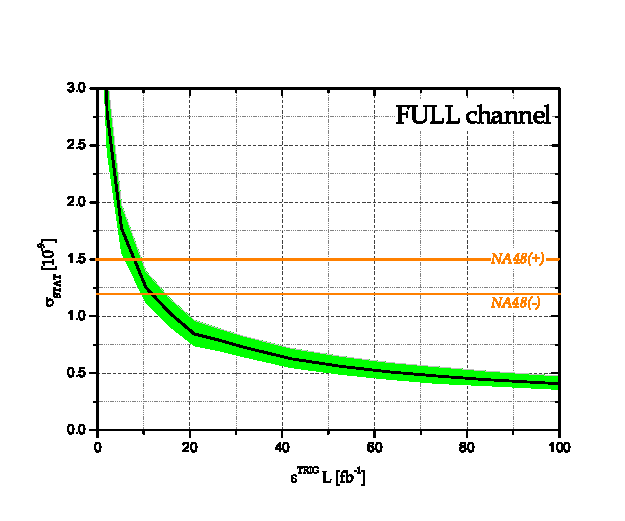
\includegraphics[scale=0.80]{figs/Kspi0MuMu/sensit_FULL.pdf}%{figs/sensitivity_more_colorfull.pdf}
\includegraphics[scale=0.80]{figs/Kspi0MuMu/sensitPARTIAL.pdf}
%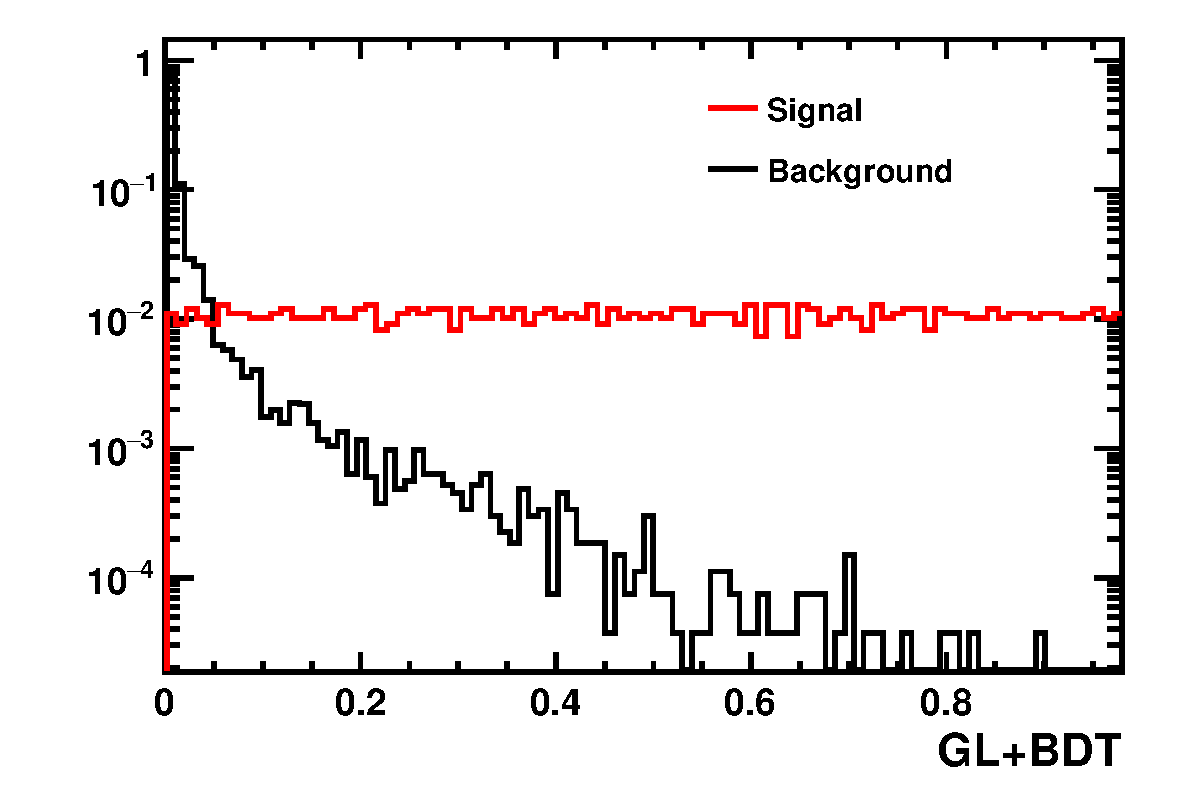
\includegraphics[scale=0.30]{figs/bdt_partial.pdf}
\caption{Expected precision on \BRof\Kspizmm for the FULL (top) and PARTIAL (bottom) channels, as a function of the integrated luminosity times trigger efficiency, $L\times\varepsilon^{TRIG/SEL}$. \label{fig:sensitivity}}
%The green line indicates the behavior of the precision extrapolating from the best fit value of the expected background. In the case of the black curve, this extrapolation is done averaging the background predictions within their uncertainties, while in the orange case the extrapolation takes as reference the best fit value of the expected background deviated one sigma from its mean value. \label{fig:sensitivity}}
\end{center}
\end{figure}


%\begin{figure} [htb!]
%\begin{center}
%\includegraphics[scale=0.60]{figs/sensitPARTIAL.pdf}
%%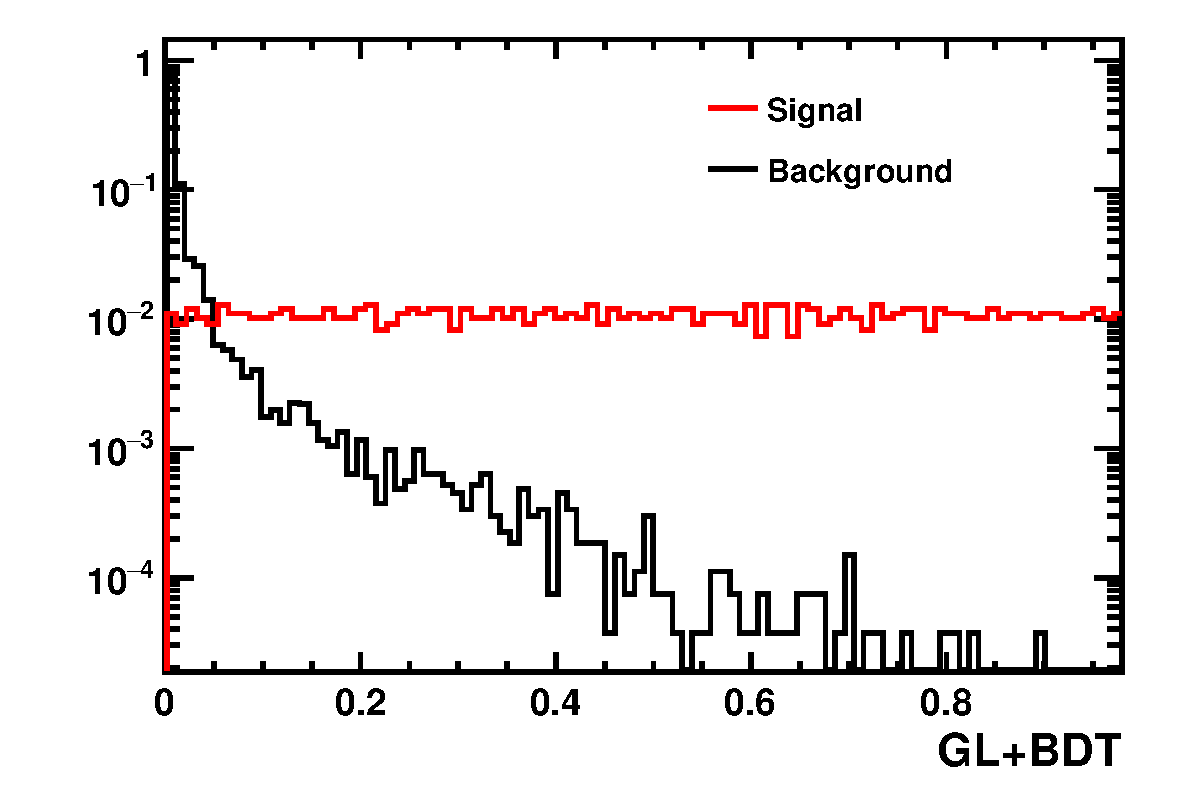
\includegraphics[scale=0.30]{figs/bdt_partial.pdf}
%\caption{Expected precision on \BRof\Kspizmm for the PARTIAL channel, as a function of the integrated luminosity times trigger efficiency, $L\times\varepsilon^{TRIG/SEL}$. The green 
%line indicates the behavior of the precision extrapolating from the best fit value of the expected background. In the case of the black curve, this extrapolation is done averaging the background 
%predictions within their uncertainties, while in the orange case the extrapolation takes as reference the best fit value of the expected background deviated one sigma from its mean value. {\it some lines are actually not there , but the plot in general needs to
%be updated} \label{fig:sensitivityPARTIAL}}
%\end{center}
%\end{figure}





 



\clearpage
% $Id: introduction.tex 87303 2016-02-08 13:44:29Z lafferty $

\subsection{Conclusions}
\label{subsec:conclusions}
A precise measurement of the \Kspizmm branching fraction is crucial for a precise ${\cal B}(\PKzL\to\Pgpz\APmuon\Pmuon)$ SM theoretical prediction and the search for physics beyond the SM in ${\PKzL}\to\Pgpz\APmuon\Pmuon$.
The sensitivity of the LHCb experiment to \BRof\Kspizmm was studied based on $3\;\rm fb^{-1}$ of data recorded at 7 and $8\;\rm TeV$ center-of-mass energy during 2011 and 2012, and on $0.3\;\rm fb^{-1}$ 
of data recorded at $13\;\rm TeV$ center-of-mass energy during 2016. Full and partial decay reconstruction algorithms were considered, aiming at 
a high reconstruction efficiency. The sensitivity study was performed using pseudo-experiments by extrapolating signal yield results based on the currently available data to expected future integrated luminosities.
If a trigger efficiency of at least 50\% can be assured in the future, LHCb can determine \BRof\Kspizmm with a precision significantly better than that of NA48.
%up to almost $10^{-10}$, which would be an improvement by an
%{\it We are the champions}

%\section*{Acknowledgements}
 
\noindent We would like to thank Gino Isidori, Giancarlo D'Ambrosio, and Ikaros Bigi for their
theoretical input. We would like to thank Teresa Fonseca for details on the NA48 analysis. 
We express our gratitude to our colleagues in the CERN
accelerator departments for the excellent performance of the LHC. We
thank the scientifical, technical and administrative staff at the LHCb
institutes. We acknowledge support from ERC, EPLANET, 
and Xunta de Galicia. We would like to dedicate this work to the memory of Pablo Rodr\'iguez.

%% $Id: introduction.tex 87303 2016-02-08 13:44:29Z lafferty $
\clearpage
\newpage
\section{Appendix: Selection and BDT}
\label{app:selection}
%{\it Fill in the details of the stripping selection, fiducial cuts
%and BDT (RoC curves, signal and backgroung histrograms of input variables ...)}

% Stripping selections

The stripping selection lines for the \KsPzMuMu and \Kspipi candidates are
\begin{itemize}
 \item StrippingK0s2Pi0MuMuLines: used for the FULL \KsPzMuMu category
 \item TriggerTestLine (in StrippingRareNStrange): used for the PARTIAL \KsPzMuMu category.
\end{itemize}
Both stripping lines use the same selection criteria for \Kspipi. 
%  \item
%  \item
%  \item Daughters must not be compatible with coming directly from the PV, by requiring a high impact parameter $\chi^2$, which is defined as the difference of the $\chi^2$ of the PV fit obtained with and without 
%  the considered track.
The stripping criteria for all lines are summarized in \tabref{stripping:pipi}. They are as follows:
\begin{itemize}
 \item The \Kspipi sample is prescaled by a factor of 0.001 due to its large size.
 \item The charged-particle containers StdAllLooseMuons and StdNoPidsPions are used.
 \item Only resolved $\pi^{0}$ candidates are used, as the merged contribute only with additional 2.9\%.
 \item \KS{}  M: \KS\ candidate mass is required to be in the range [400, 600] \mevcc{} for the FULL and \Kspipi samples.
 \item $\mu^{+}\mu^{-}$  M: The dimuon candidate mass for the PARTIAL sample is required to be smaller than 450 \mevcc to reduce the contribution from misidentified \Kspipi. This is a loose requirement,
       given that the maximum dimuon mass, without considering the detector response, is $m_{\KS}-m_{\pi^{0}}=362$ \mevcc.
 \item \KS{} tof: Proper decay time of the \KS\ candidate given in a fraction of the \KS\ lifetime. This variable is computed using the reconstructed momentum of the \KS candidate and the distance between 
      the reconstructed secondary (SV) and primary (PV) vertices.
 \item \KS{} IP:  The \KS\ candidate must be compatible with the PV, asking for a low impact parameter with respect to PV.
 \item $\mu^{+}\mu^{-}$ DIRA: Forward \KS\ decay, requiring a positive cosine of the polar direction angle (DIRA).
 \item $\mu^{+}\mu^{-}$ DOCA: Good reconstruction quality of the SV required asking for a low distance of closest approach (DOCA) of the two daughter tracks.
 \item Daug. Track $\chi^{2}/ndof$:  Good reconstruction quality of the muon/pion tracks is required using the $\chi^{2}/ndof$ of the track fit. This is the standard cut of long tracks in LHCb.

 \item Daug. IP$_{\chi^{2}}$ : Daughters must not be compatible with coming directly from the PV, by requiring a high impact parameter $\chi^{2}$, which is defined as the difference of the $\chi^{2}$ of the PV
       fit obtained with and without the considered track.
 \item Daug. Track ghost prob.:  accounts for the probability that a track does not correspond to a track from a single charged particle.
 \item Daug. PID: The DLL $\mu-\pi$ ($log(P_{\mu}/P_{pi})$) is used to increase the muon purity at stripping level.
 \item Vertex $\rho$: The radial distance between the dimuon vertex in LHCb coordinates.
 \item Vertex $z$: The distance in $z$ (LHCb coordinates).
 \item Vertex $\chi^{2}/ndof$: A good-quality vertex is assured by placing a requirement on its fit quality.
 \item $\delta_{z}$: Distance from the end vertex of the particle and the related primary vertex.
 \item $\cos\alpha$: Cosine of the angle between the \KS\ momentum and the direction fo flight from the best PV to the decay vertex.
 \item IP$_{\text{max}}$/$\delta_{z}$.
\end{itemize}

\begin{table}[!ht]
\centering
\begin{tabular}{l@{\hspace{0.5cm}}l@{\hspace{0.5cm}}l@{\hspace{0.5cm}}l}
\hline
\textbf{Variables}                & $\boldsymbol{\Kspizmm}$ & $\boldsymbol{\Kspizmm}$ &$\boldsymbol{\Kspipi}$  \\
				  & {\bf FULL} &  {\bf PARTIAL} &  \\
\hline
Stripping line			  & K0s2Pi0MuMuLines & TriggerTestLine & K0s2Pi0MuMuLines\\
			          & & & RareNStrange\\
Prescale			  & 1 & 1 & 0.001\\
Input Particles              	  & StdAllLooseMuons & StdAllLooseMuons & StdNoPidsPions   \\
                                  & StdLooseResolvedPi0 & &   \\
\KS{}  M                          & [400, 600] \mevcc{}  & - & [400, 600] \mevcc{}    \\
$\mu^{+}\mu^{-}$  M               & -  & $<$ 450 \mevcc{} &     \\
\KS{}  tof                        & $>$ 0.06$\tau$ & $>$ 0.06$\tau$ & $>$ 0.1$\tau$  \\
\KS{}  IP                         & $< 0.9$ \small mm &  - & $< 0.4$ \small mm    \\
$\mu^{+}\mu^{-}$ DIRA             & $>$ 0 \small s & $>$ 0  \small s &  $>$ 0  \small s\\
$\mu^{+}\mu^{-}$ DOCA            & $<$ 0.3 \small mm  & $<$ 0.1 \small mm  &  $<$ 0.3 \small mm     \\
Daug. Track $\chi^{2}/ndof$   	  & $<$ 5 & $<$5 &  $<$ 5          \\
Daug. IP$_{\chi^{2}}$         	  & $>$ 36 & $>$ 60 &  $>$ 100        \\
Daug. Track ghost prob.        	  & - & $<$ 0.1 &  -        \\
Daug. PID        	  	  & - & $>$ 0 &  -        \\
Vertex $\rho$        	  	  & - & $>$ 4 \small mm&  -        \\
Vertex $z$        	  	  & - & $>$ 650 \small mm &  -        \\
Vertex $\chi^{2}/ndof$        	  	  & - & $<$ 9 &  -        \\
$\delta_{z}$    		  & - & $>$ 0 \small mm &  -        \\
$\cos\alpha$    		  & - & $>$ 0  &  -        \\
IP$_{\text{max}}$/$\delta_{z}$    & - & $<$ 1/60 s$^{-1}$&  -        \\
\hline
\end{tabular}
\caption[Stripping selection]{The \Kspizmm and \Kspipi selection cuts performed in the stripping phase.
The definitions of the variables is given in the text.}
\label{stripping:pipi}
\end{table}

The candidates were selected using three Strippings: 
\begin{itemize}
\item Stripping 21: used for 2011/2012 data
% \item Stripping 24: used for 2015 data
\item Stripping 26: used for 2016 data.
\end{itemize}

The PARTIAL analisys is tested in Stp26, while the FULL is tested in Stp21.
% BDT  (variables, RoC curves, signal and background histograms of input variables)

Before the training, the following cuts are made on the data to reduce the amount of background (while keeping most of the signal):
\begin{itemize}
\item Number of hits in the Trigger Tracker greater than 0.1 for both muons
\item ProbNNmu greater than 0.05 
\item Lifetime of the \KS greater than 1 ps
\item Invariant mass of the decay result smaller than 490 \mev
\item Kinematic cut in the Armenteros-Podolanski plane, removing $\Lambda\to p \pi$ and $\KS\to \pi^{+}\pi^{-}$ 
\end{itemize}
The input MVA variables used are divided into continuous variables and discrete variables. The continuous variables are gaussianized, decorrelated, and gaussianized again. Then the gaussianized and the discrete 
variables are inputs for the BDT training. 
% {\it put table with cuts and values, as well as names of the containers of the input particles}
The set of variables common to the FULL and PARTIAL cases consists of:
\begin{itemize}
\item Distance of closest approach (DOCA)
\item \KS flight distance significance. 
\item $\chi^2$ of $\mu$ track fit
%\item Muon impact parameter
\item Vertex $\chi^2$
%\item ProbNNmu: probability for the muon to be a real muon instead of another particle
\item \KS $p_T$ 
\item \KS impact parameter significance (difference in the $\chi^2$ of the fit of the vertex obtained with and without the introduction of the track in the fit)
\item Impact parameter significance of the muons with respect to any PV in the event
\item PID variables for muons
\end{itemize}


\begin{itemize}
\item Hits in VELO 
\item Hits in Inner Tracker
\item Hits in Trigger Tracker
\item Hits in Outer Tracker
\item Secondary Vertex coordinates 
\end{itemize}

Apart from these, there are inputs that are specifically used for FULL. \\

\textbf{FULL:}

\begin{itemize} %FULL
\item Angle between $\mu \mu$ and $\gamma\gamma$ planes
\item \Pgpz mass
\item Helicity angles (as defined in \figref{fig:angles}). 
\end{itemize}


\begin{figure} [htb!]
\begin{center}
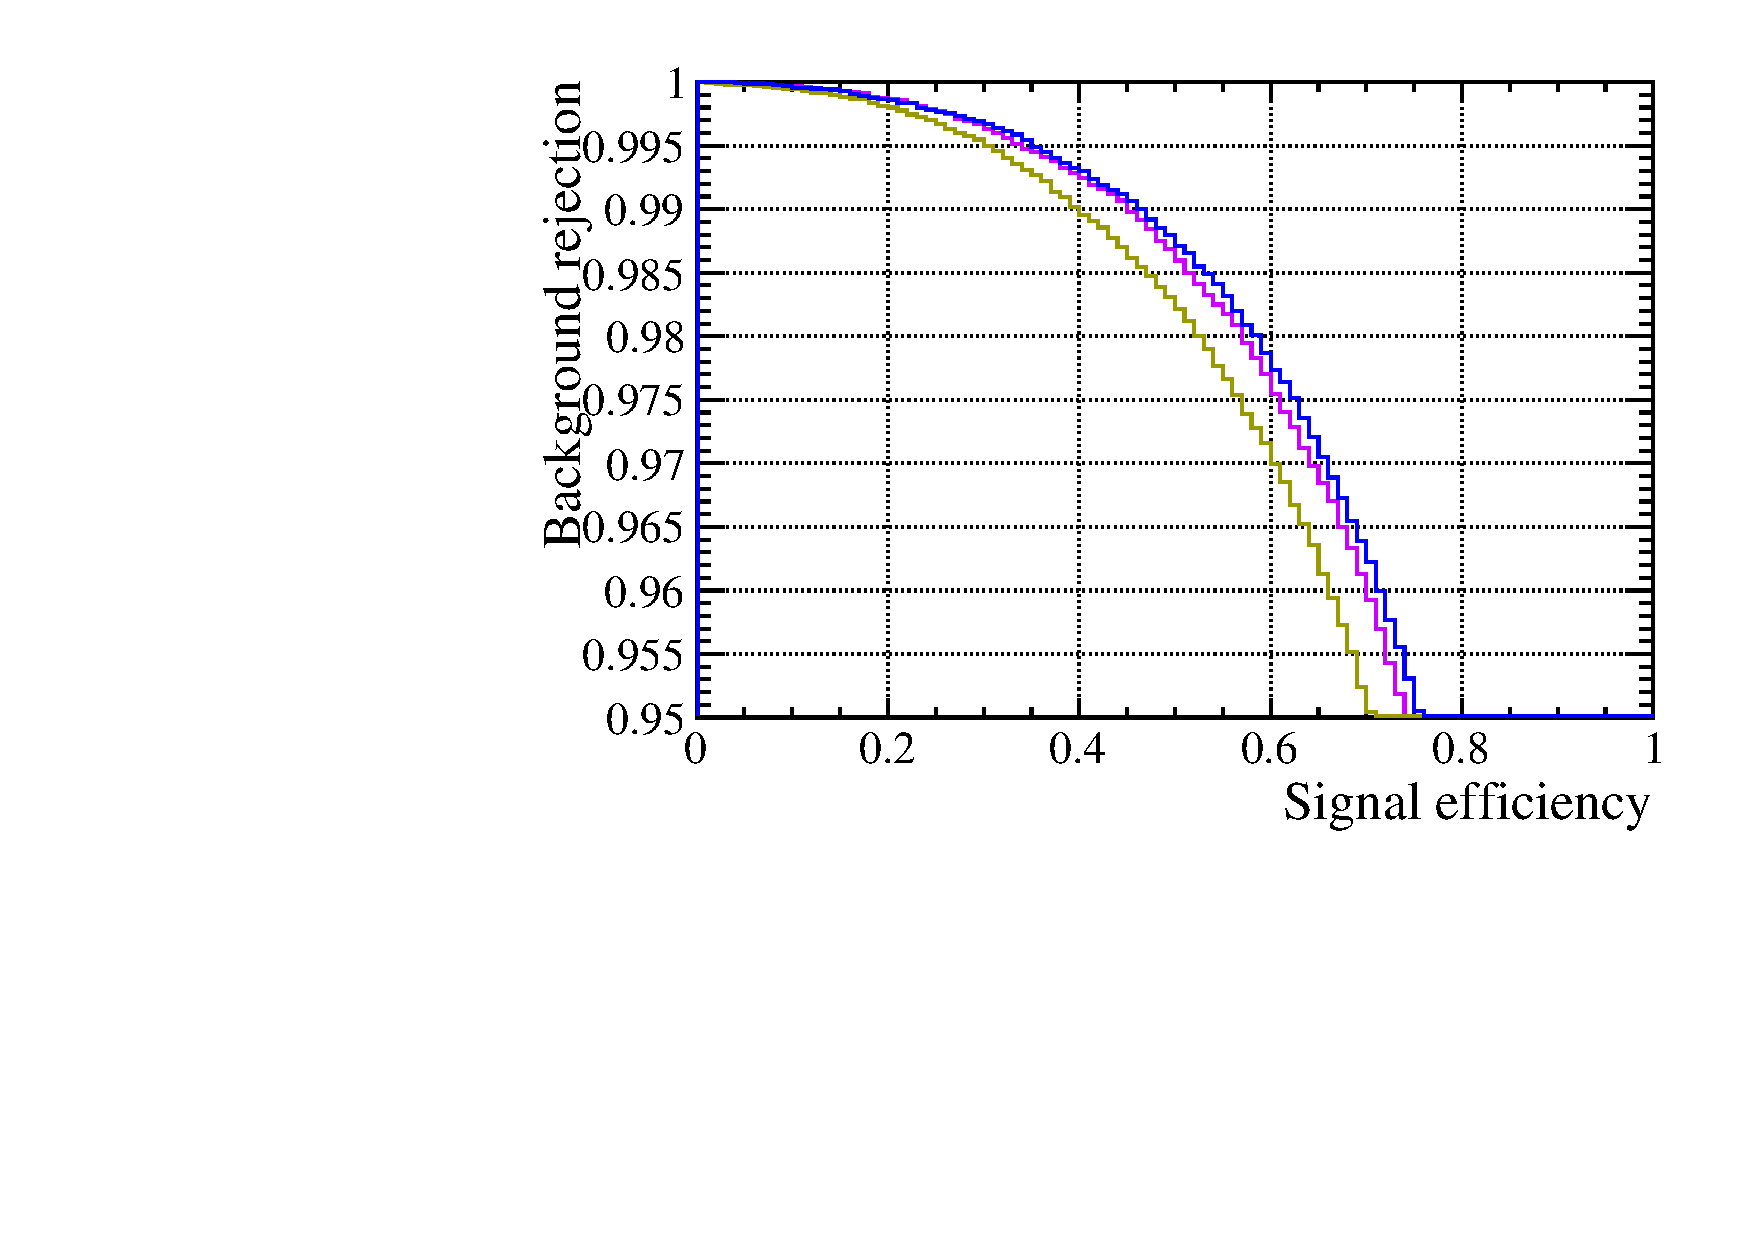
\includegraphics[scale=0.50]{figs/GL_BDT_Kspi0_pi0.pdf}
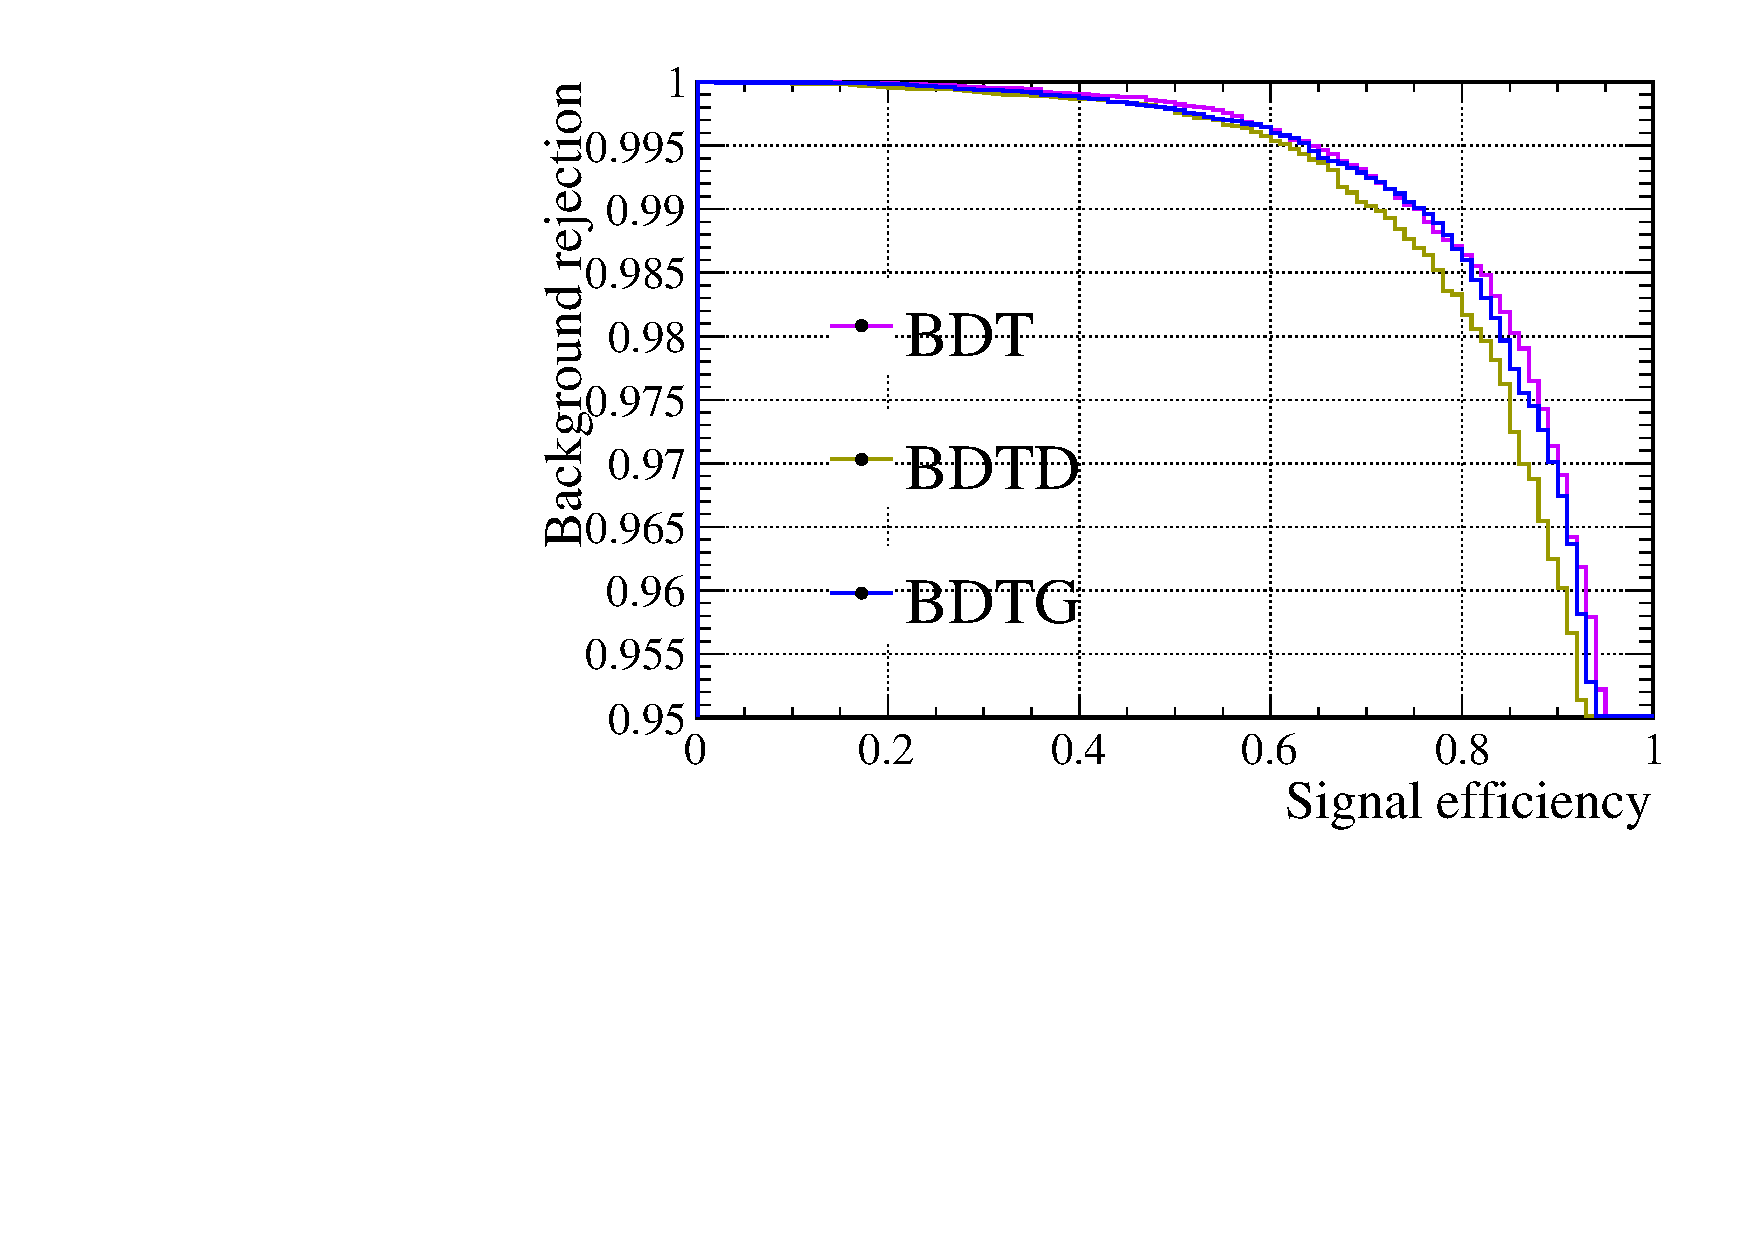
\includegraphics[scale=0.50]{figs/ROC_PARTIAL_noGhost.pdf}%GL_BDT_Kspi0_nopi0_VC.pdf}
\caption{ROC curves for the FULL (top) and PARTIAL (bottom) categories.  \label{fig:ROC}} % TODO \textcolor{red}{Resize, remove BDTB}
\end{center}

\end{figure}

%Signal and background histograms of input variables (plots for input variable distributions)
The ROC (Receiver Operating Characteristic) curves obtained for both cases are represented in \figref{fig:ROC}. 
Finally, in \figref{fig:MVAhistos_FULL1}, \figref{fig:MVAhistos_FULL2} and \figref{fig:MVAhistos_PARTIAL} the histograms for signal and background of the BDT input variable distributions are shown for the 
FULL and PARTIAL categories, respectively. 
We find that the fraction of MC signal \KS coming from $b$ or $c$ decays
is less than a per mil.

\begin{figure} [htb!]
\begin{center}
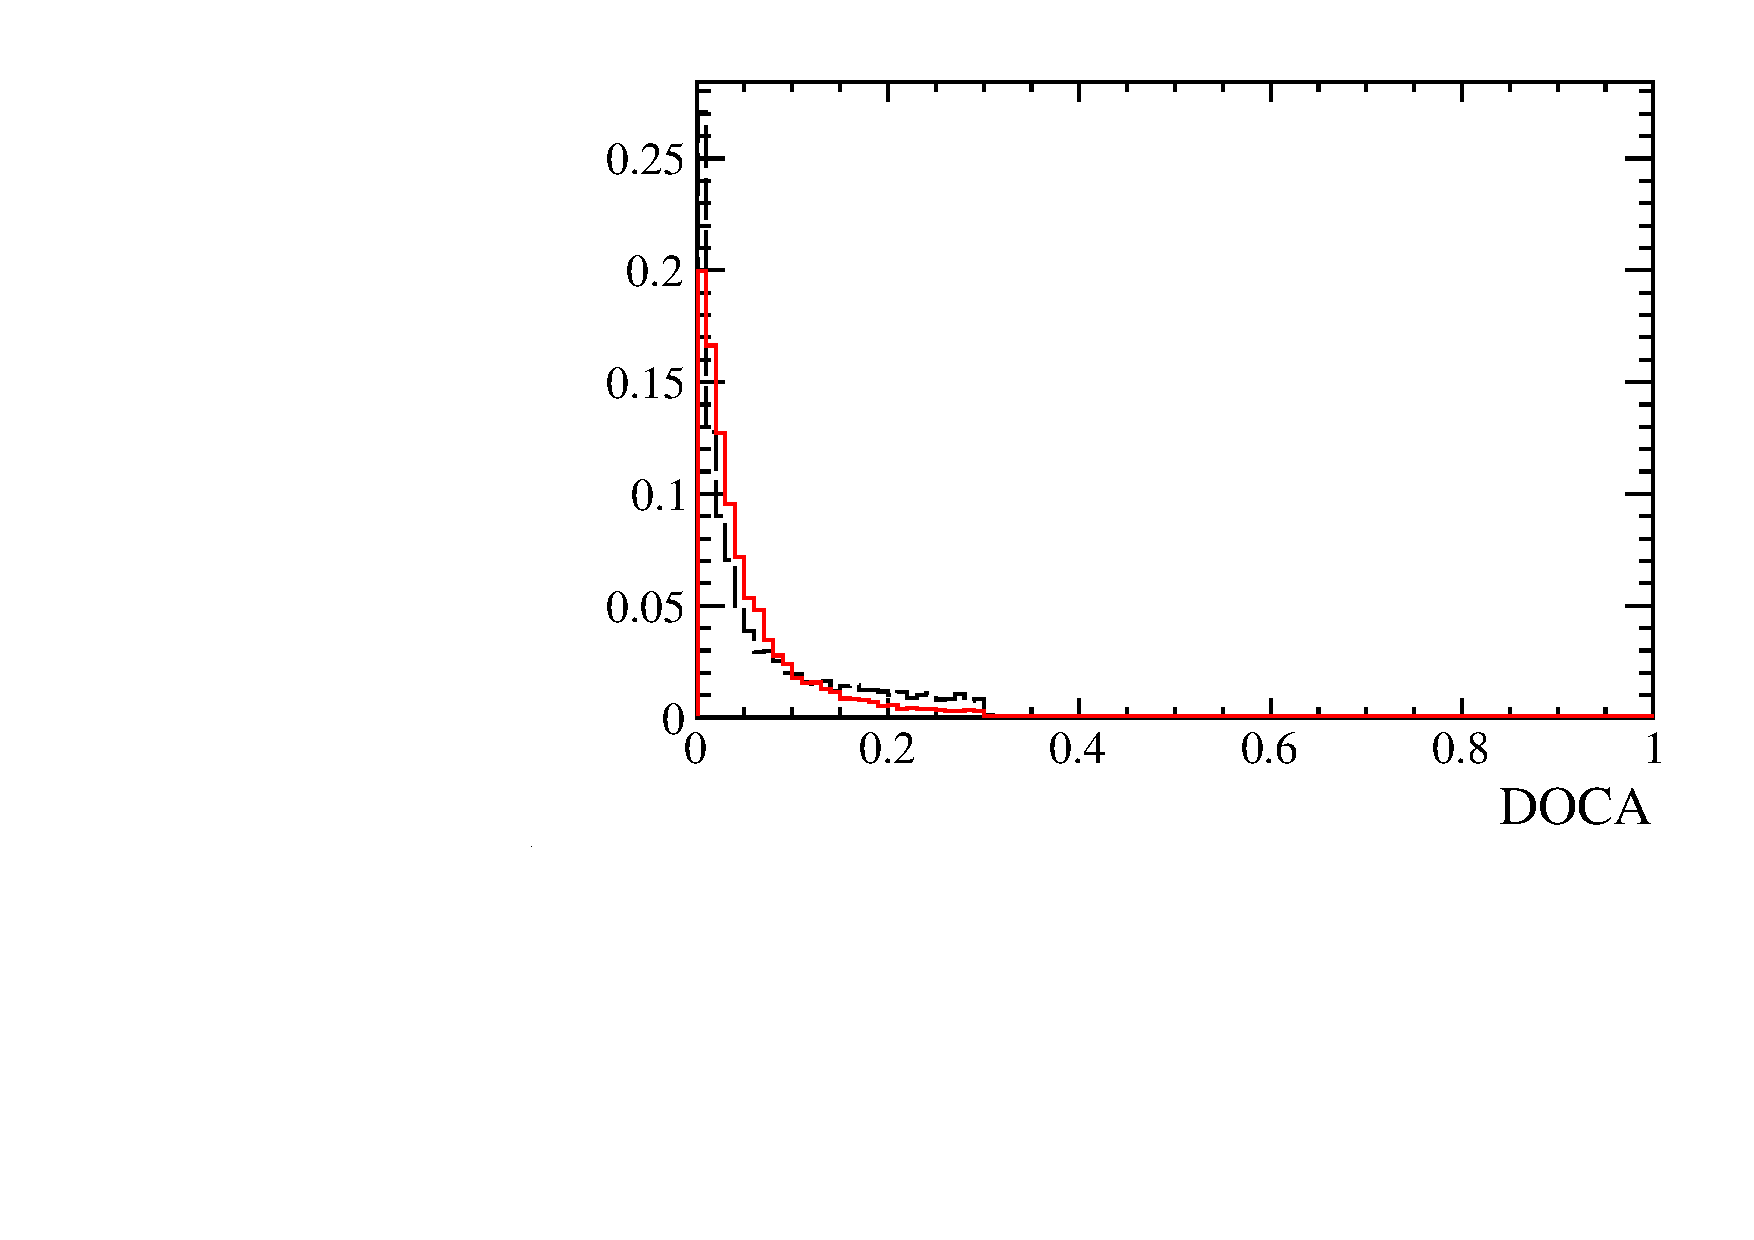
\includegraphics[scale=0.20]{figs/DOCAFULL.pdf}
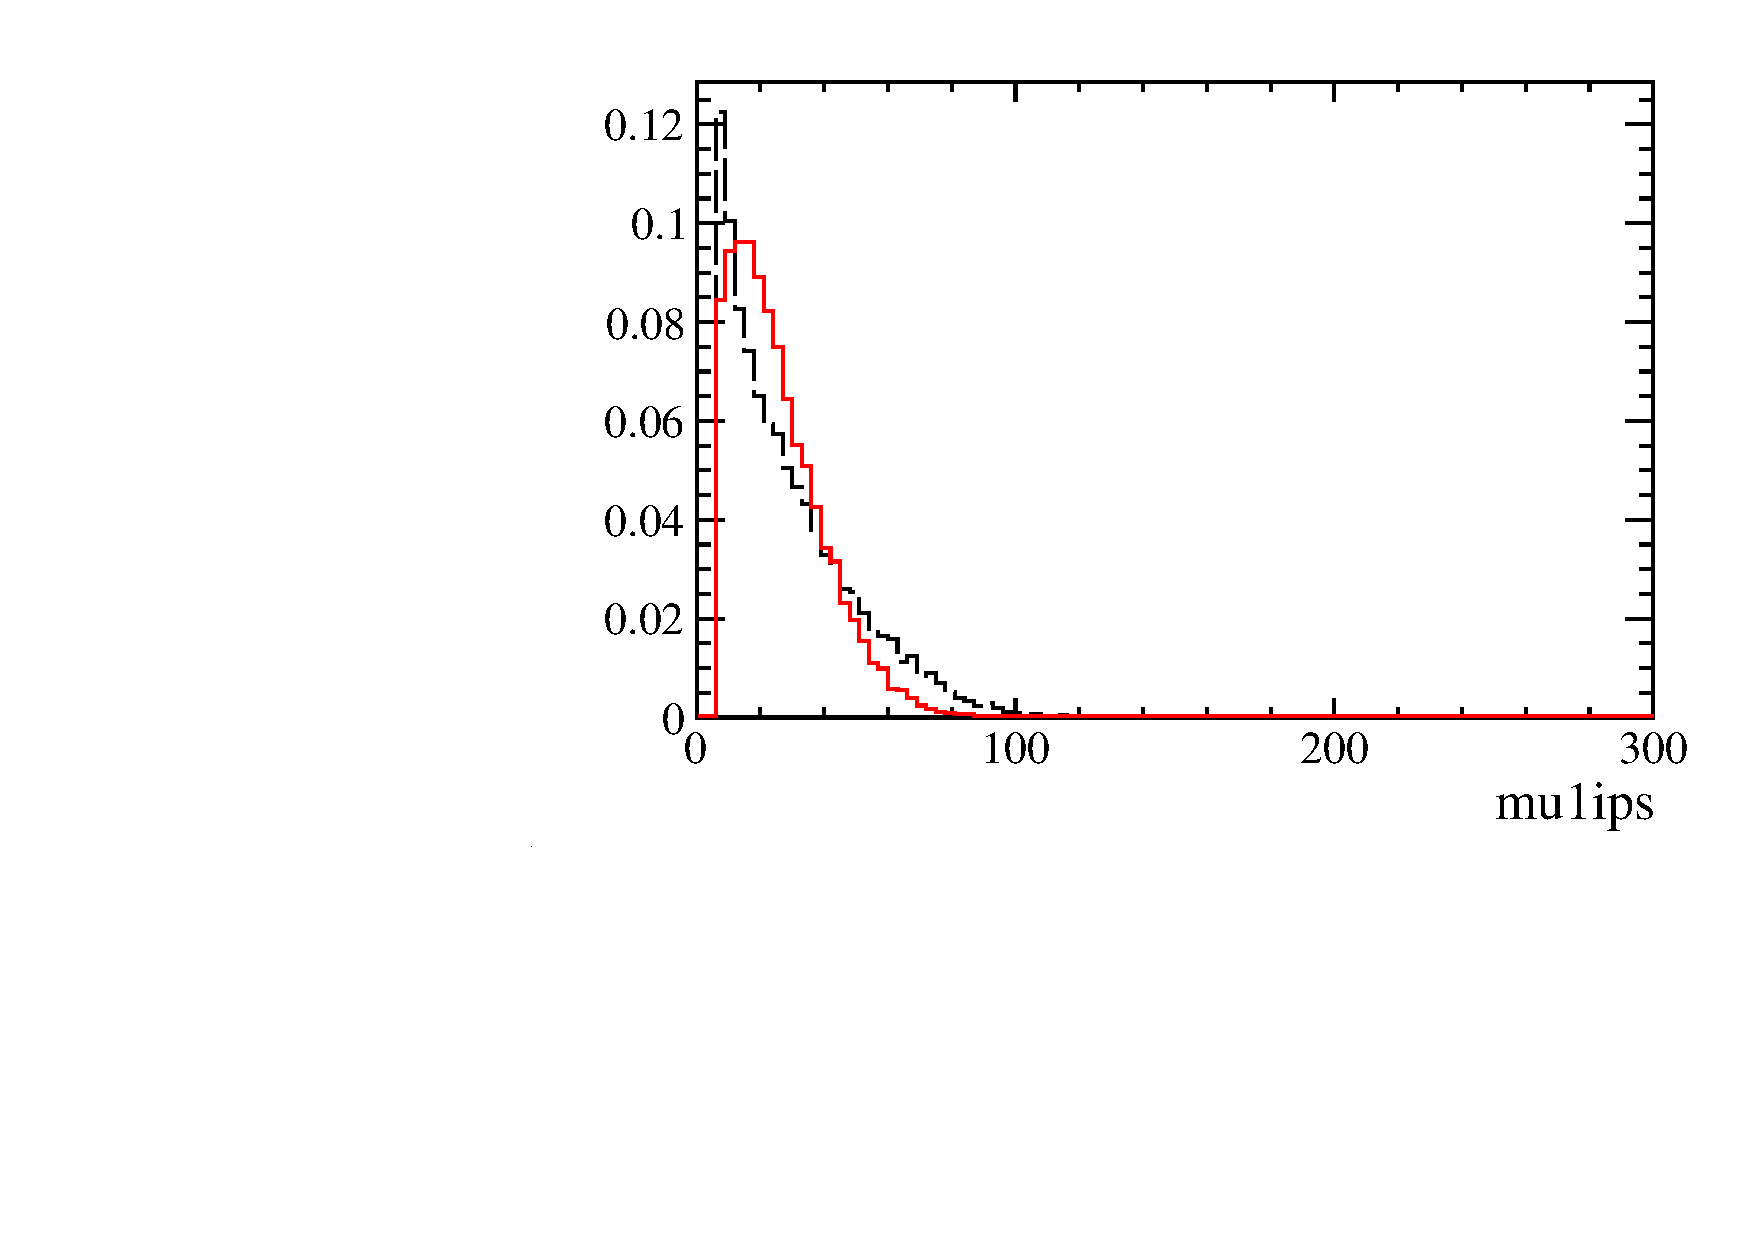
\includegraphics[scale=0.20]{figs/mu1ipsFULL.pdf}
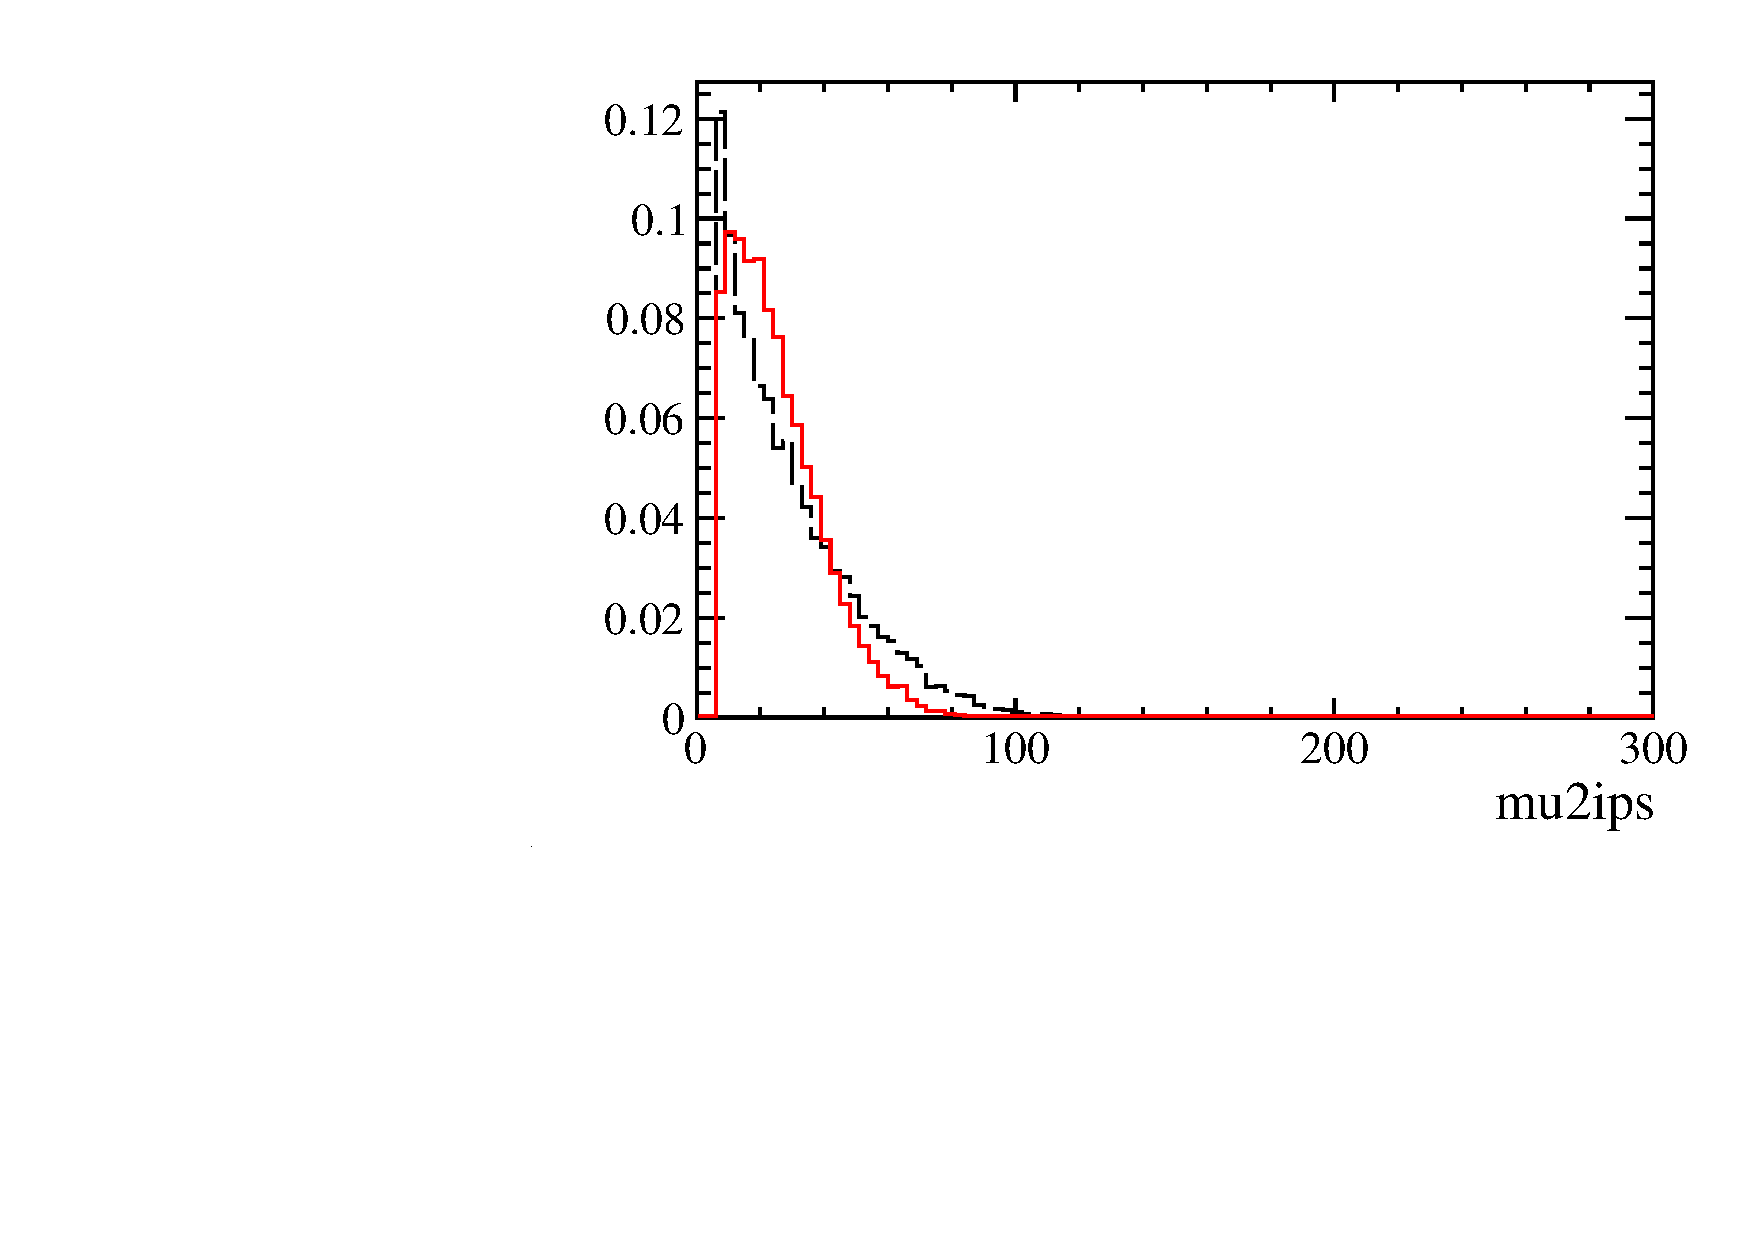
\includegraphics[scale=0.20]{figs/mu2ipsFULL.pdf}
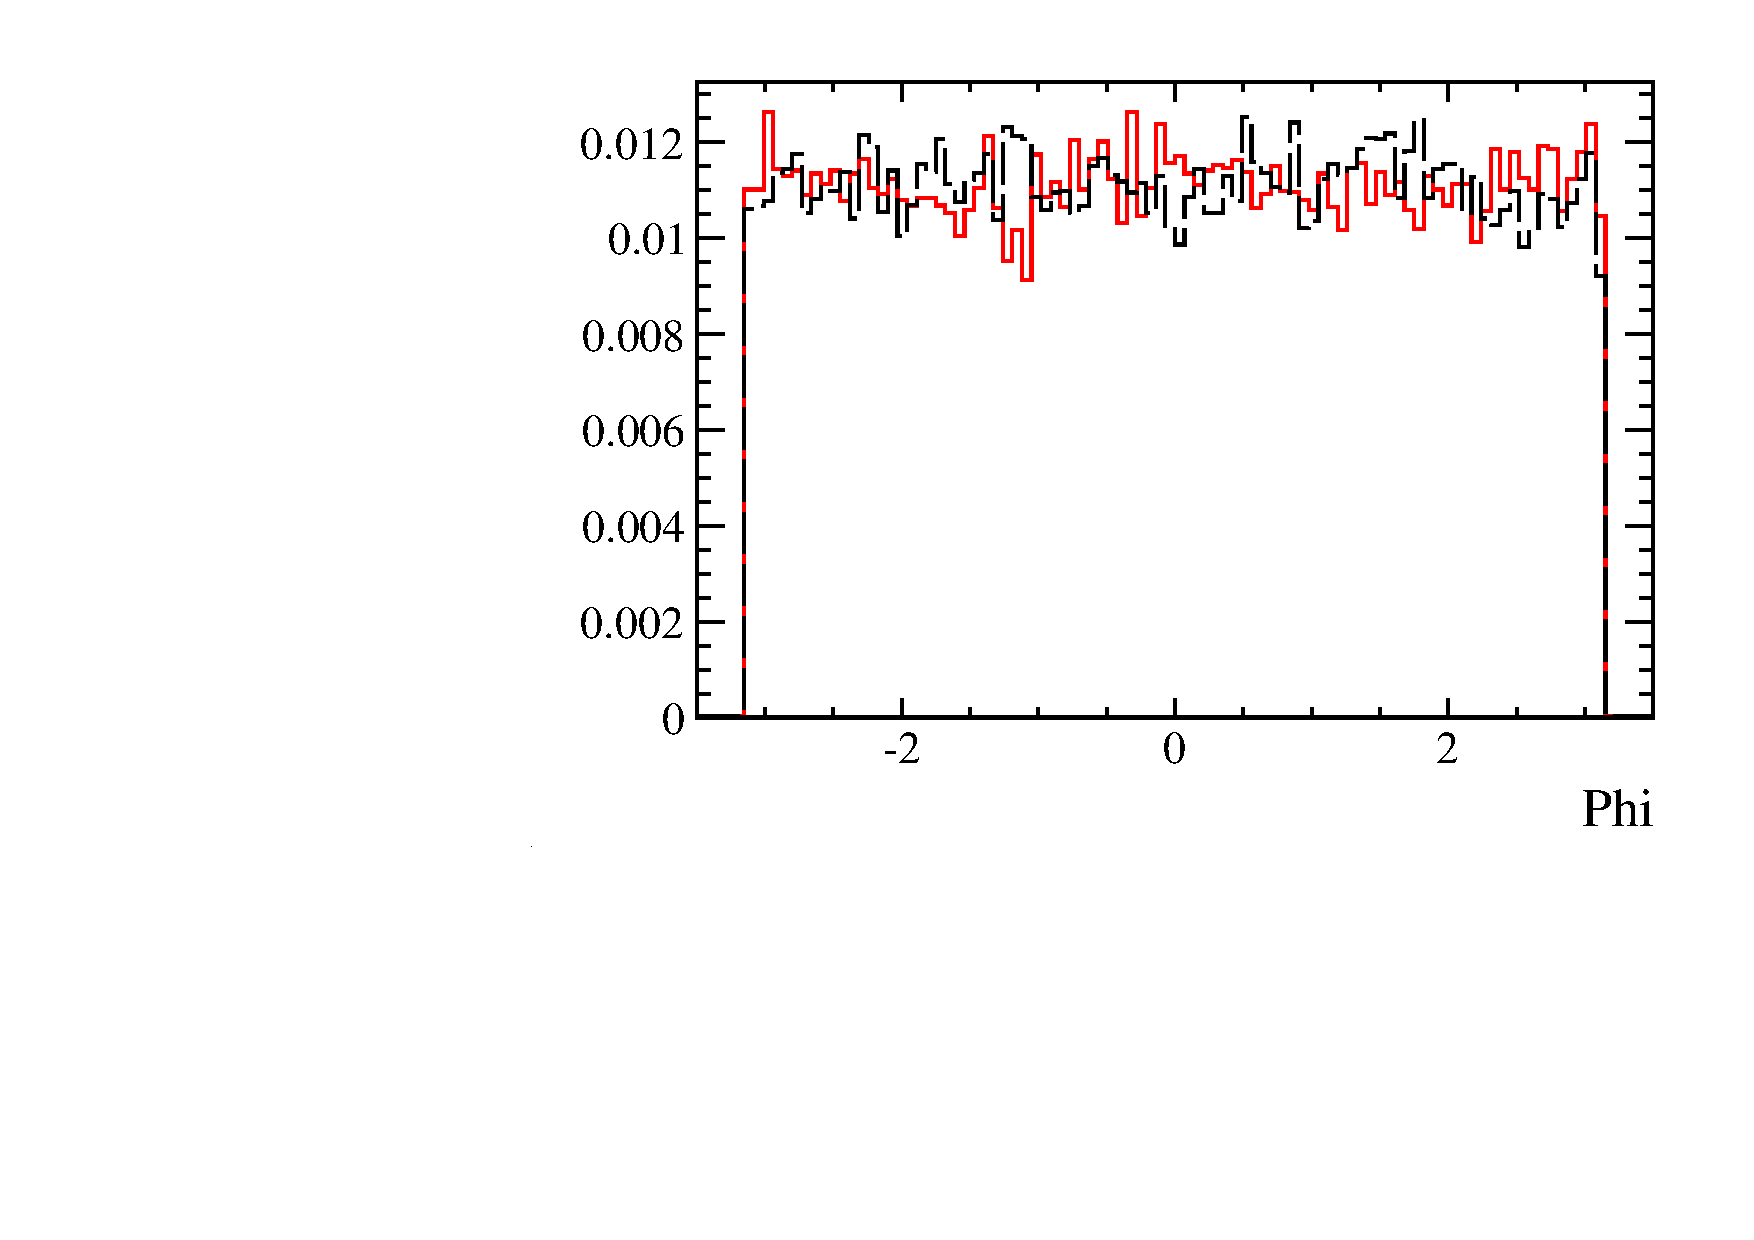
\includegraphics[scale=0.20]{figs/PhiFULL.pdf}
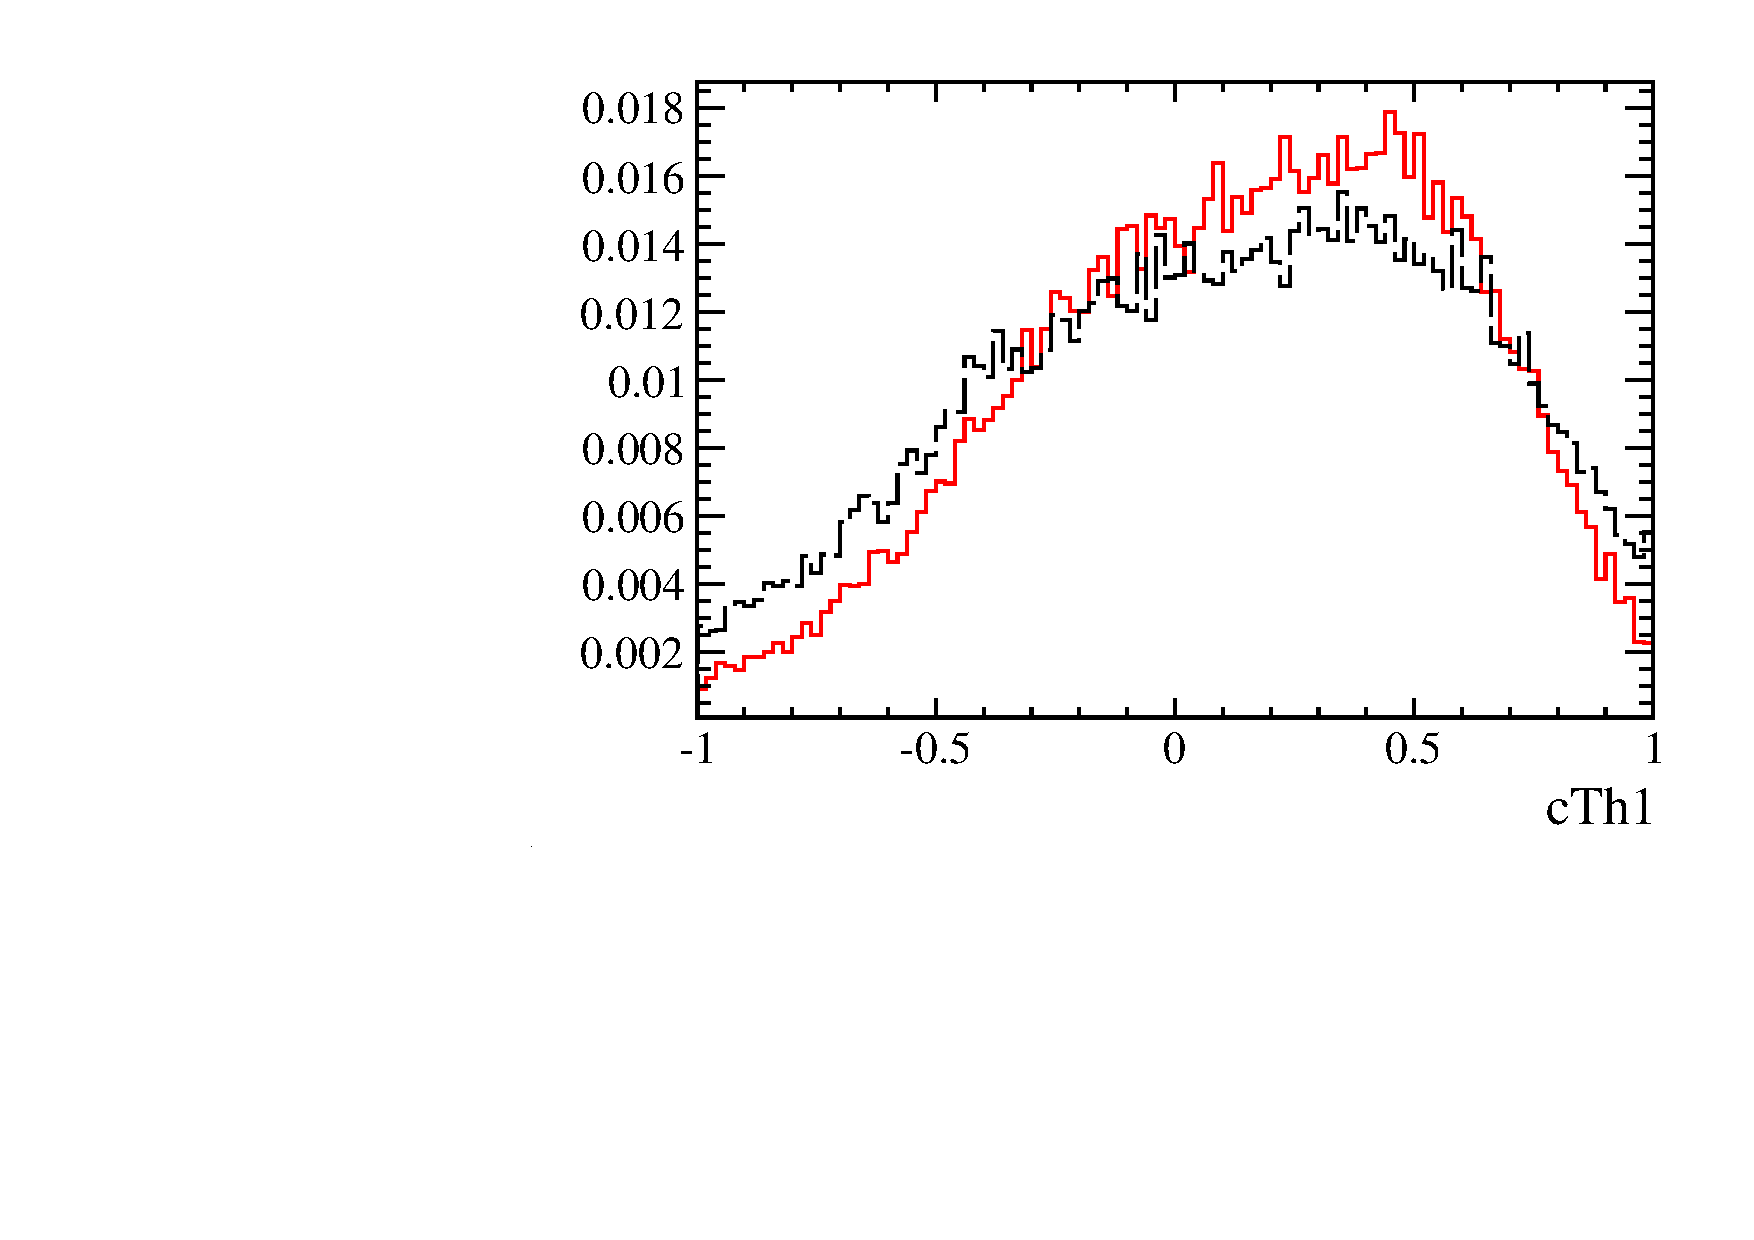
\includegraphics[scale=0.20]{figs/cTh1FULL.pdf}
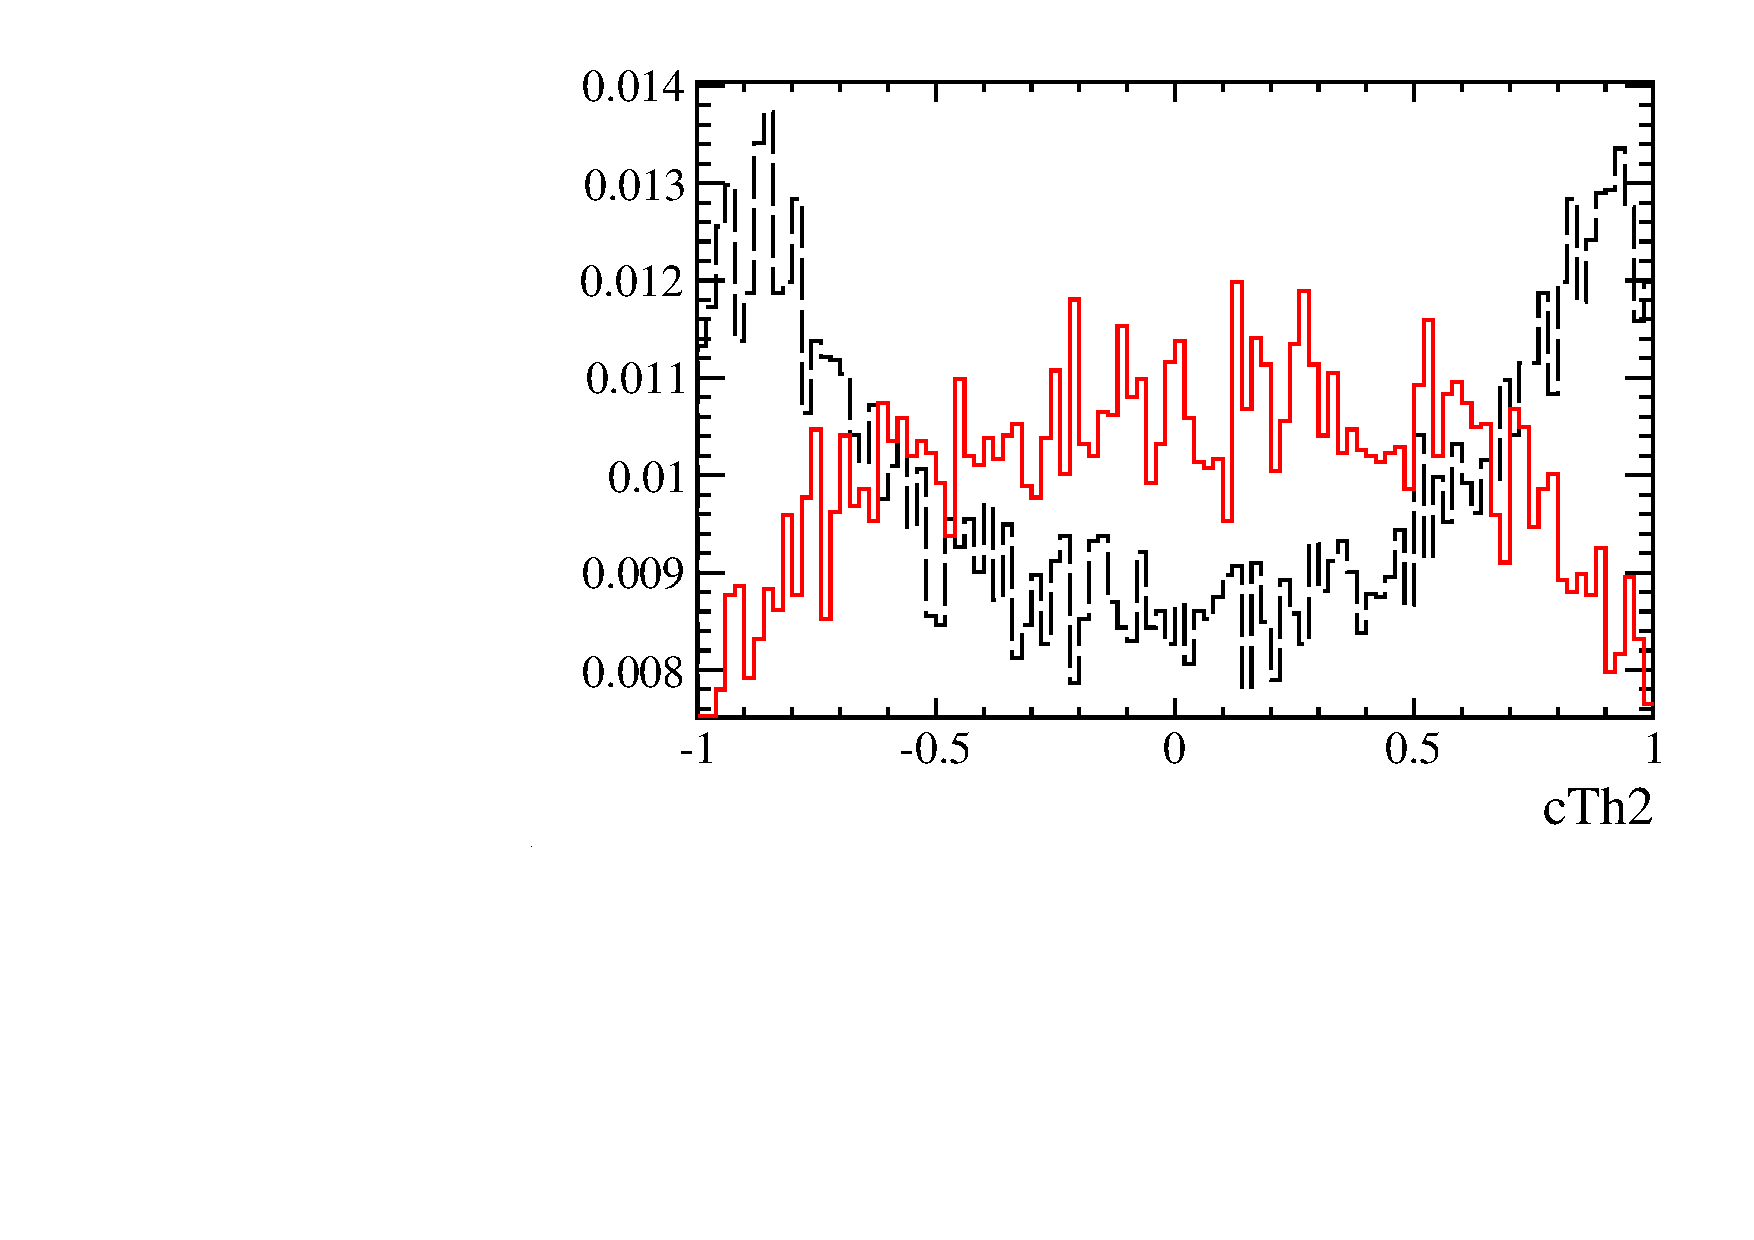
\includegraphics[scale=0.20]{figs/cTh2FULL.pdf}
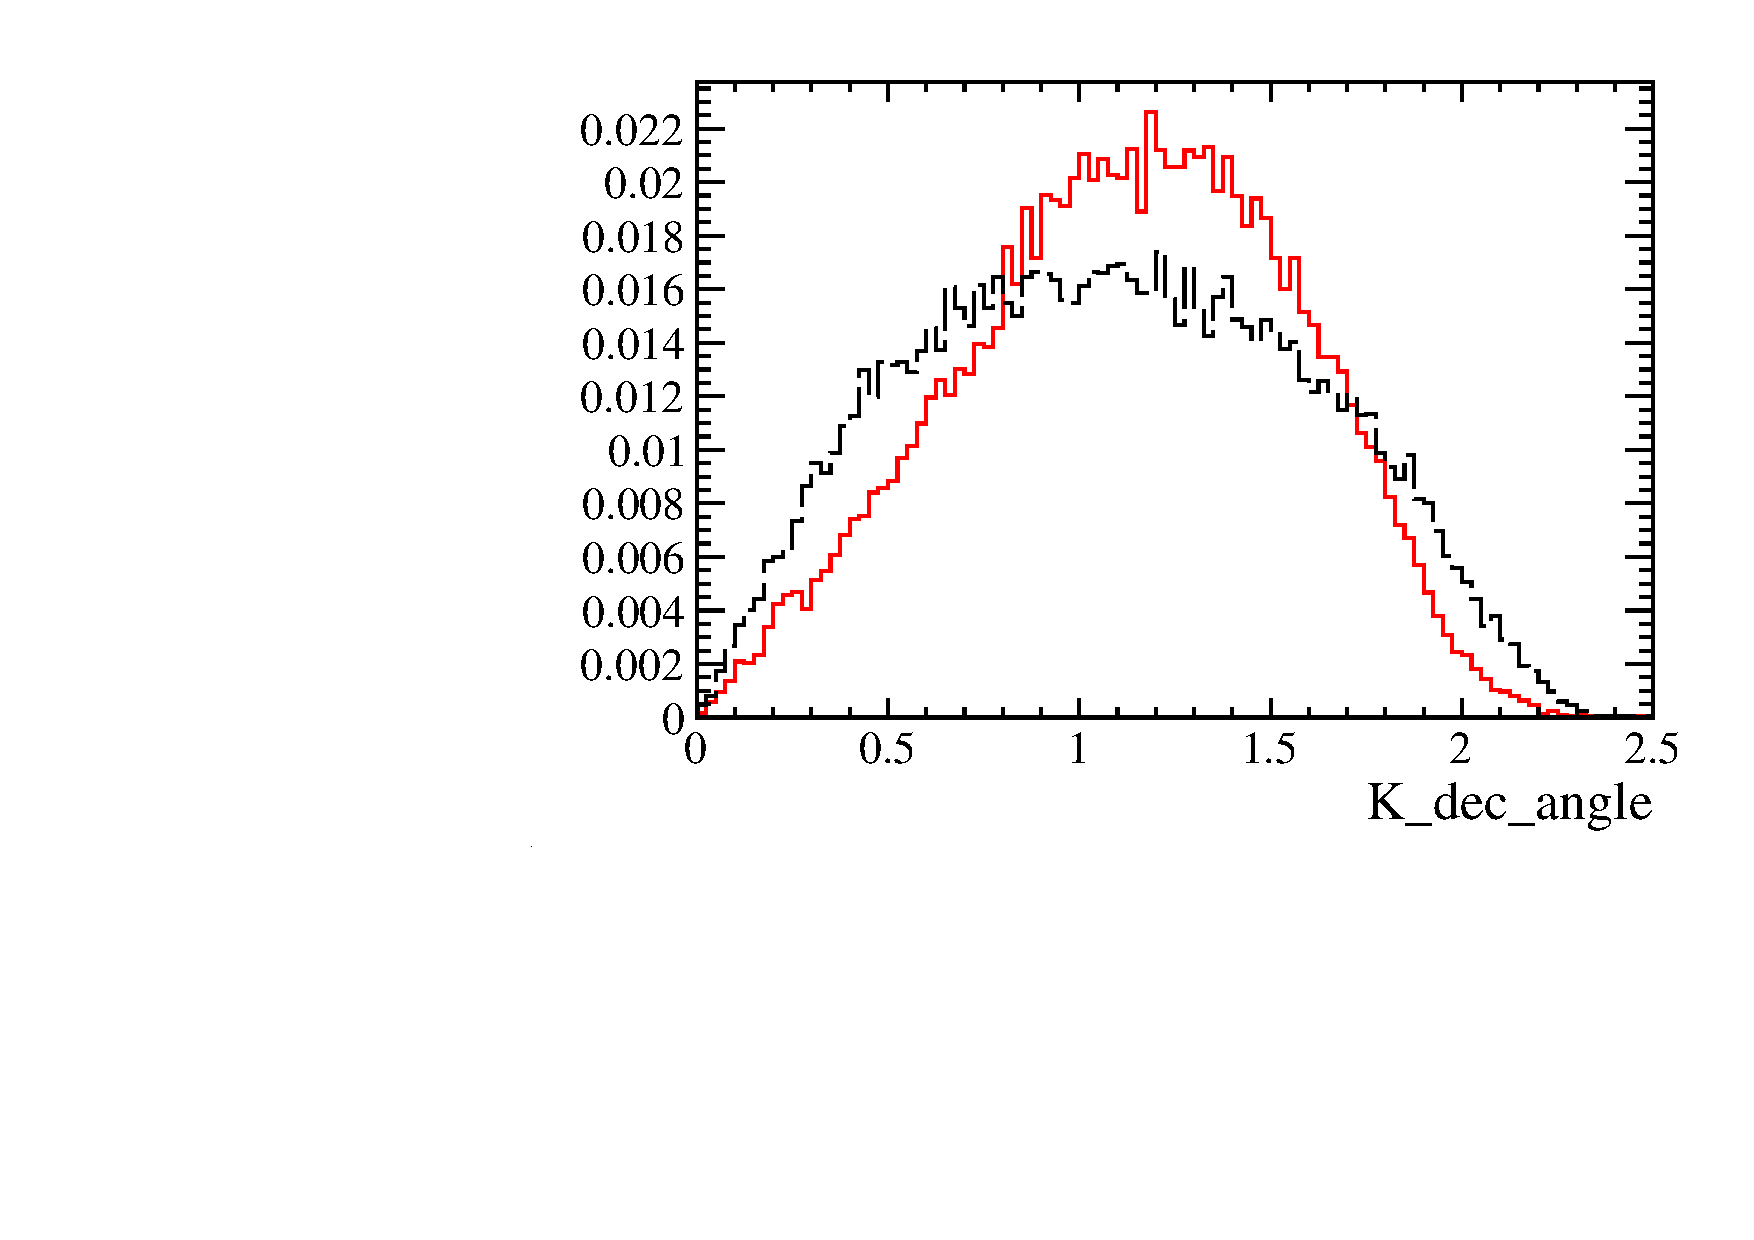
\includegraphics[scale=0.20]{figs/K_dec_angleFULL.pdf}
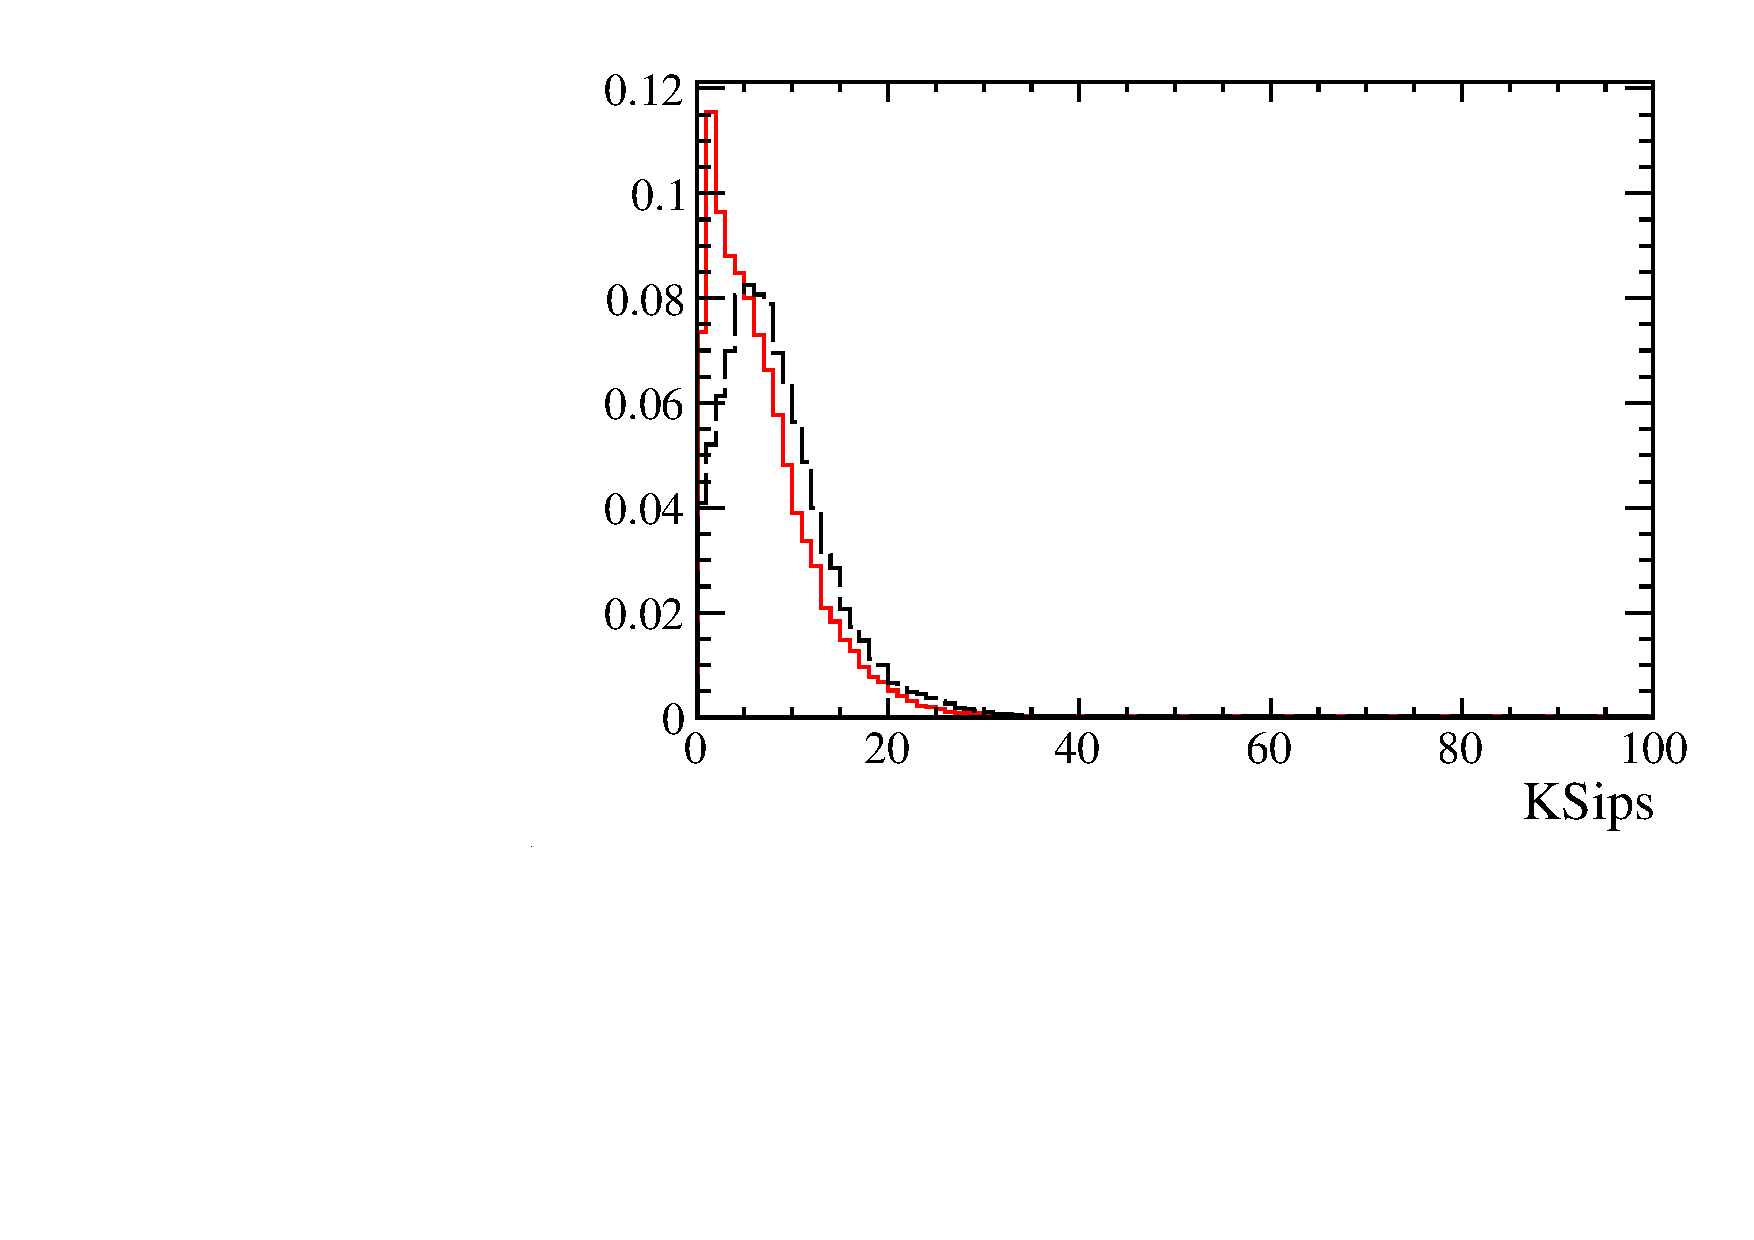
\includegraphics[scale=0.20]{figs/KSipsFULL.pdf}
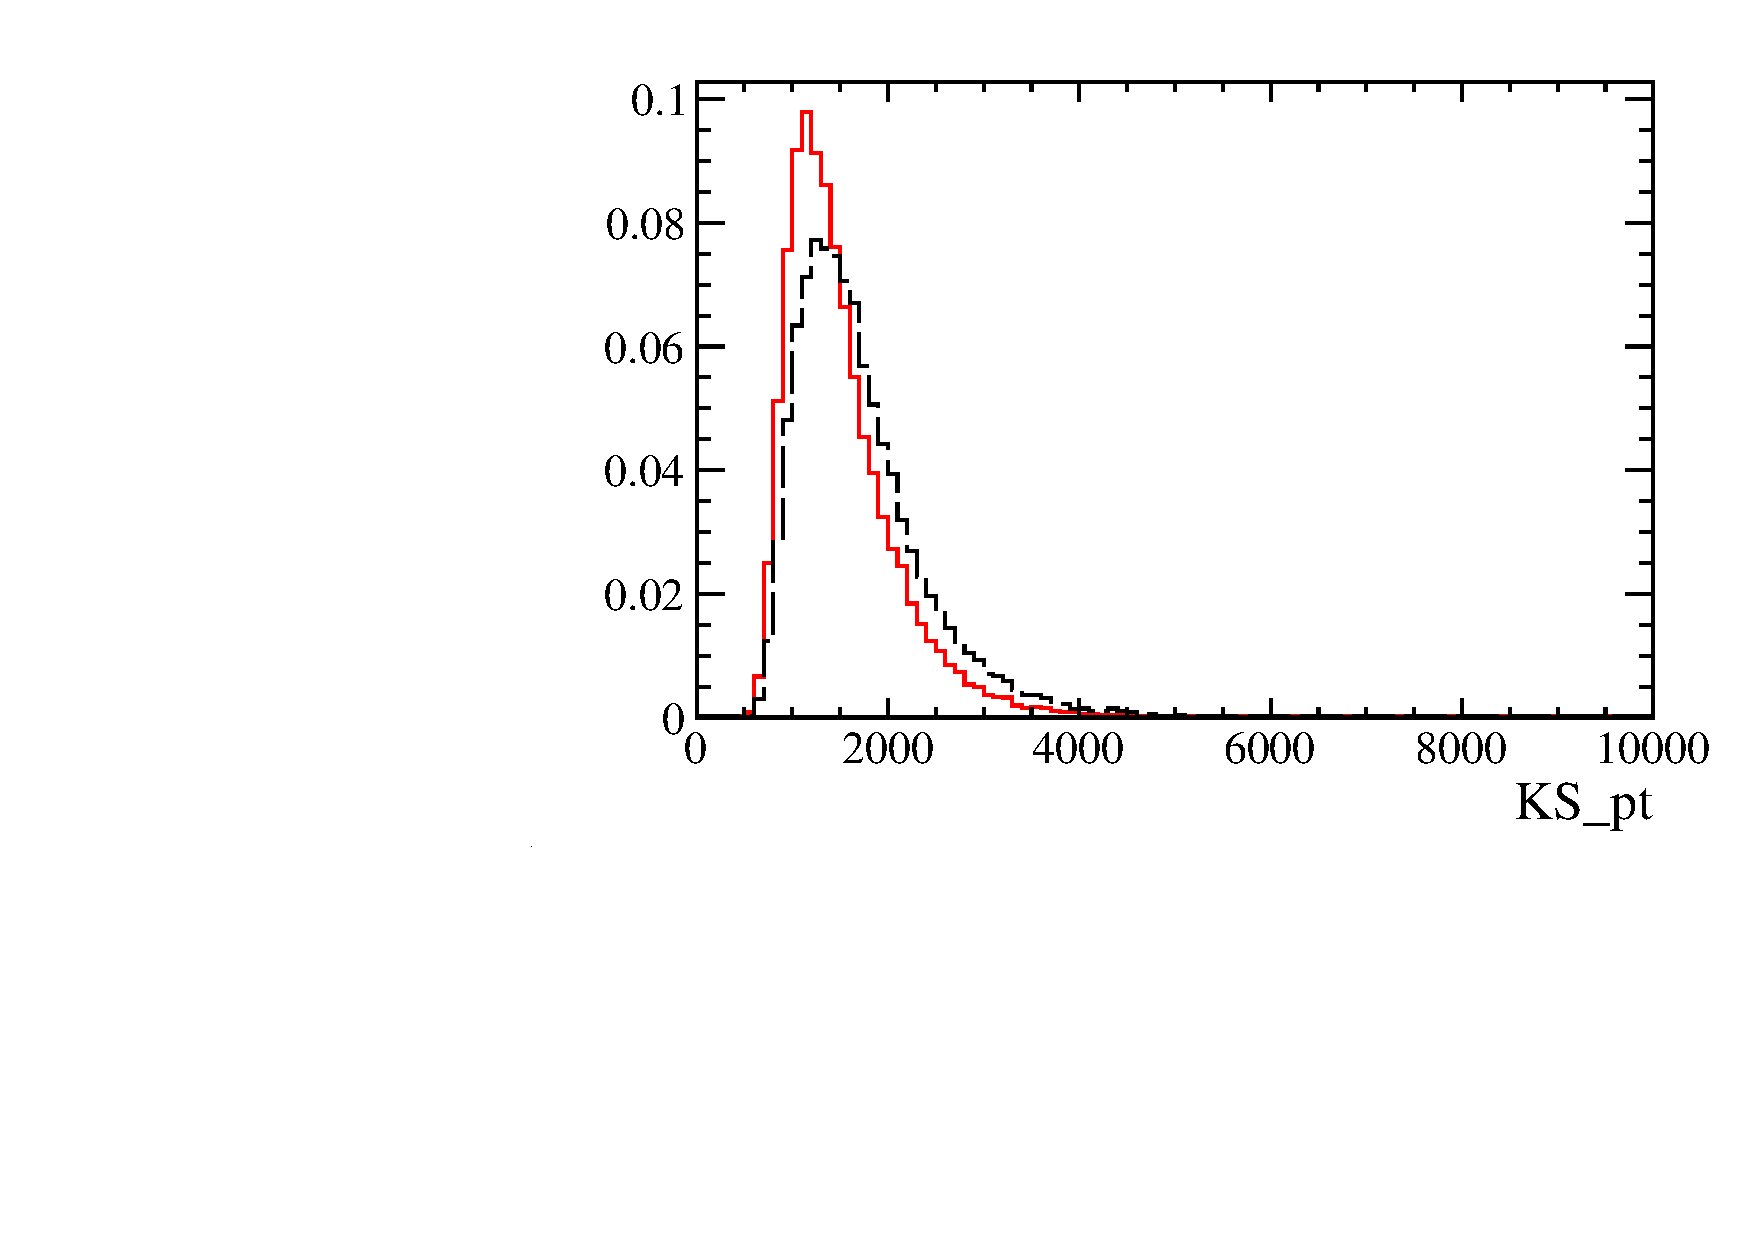
\includegraphics[scale=0.20]{figs/KS_ptFULL.pdf}
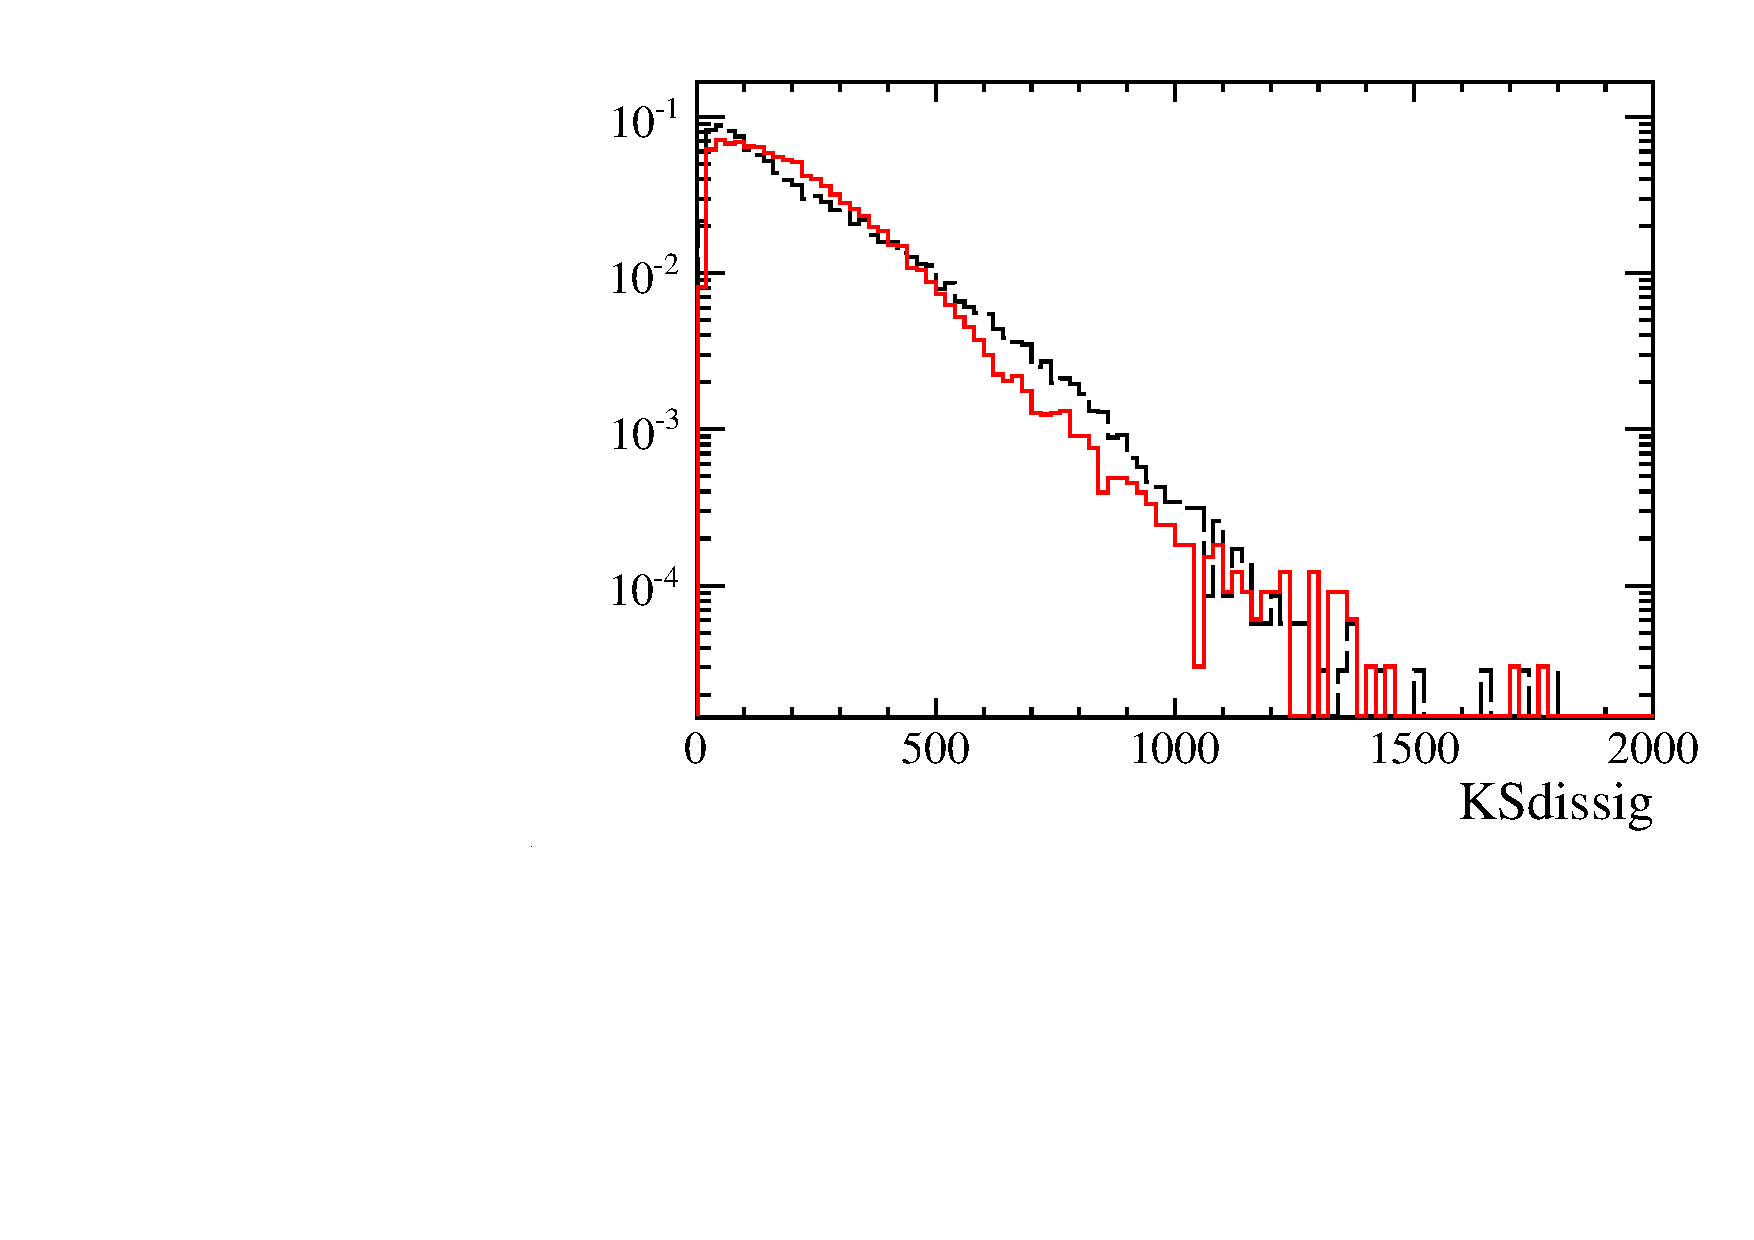
\includegraphics[scale=0.20]{figs/KSdissigFULL.pdf}
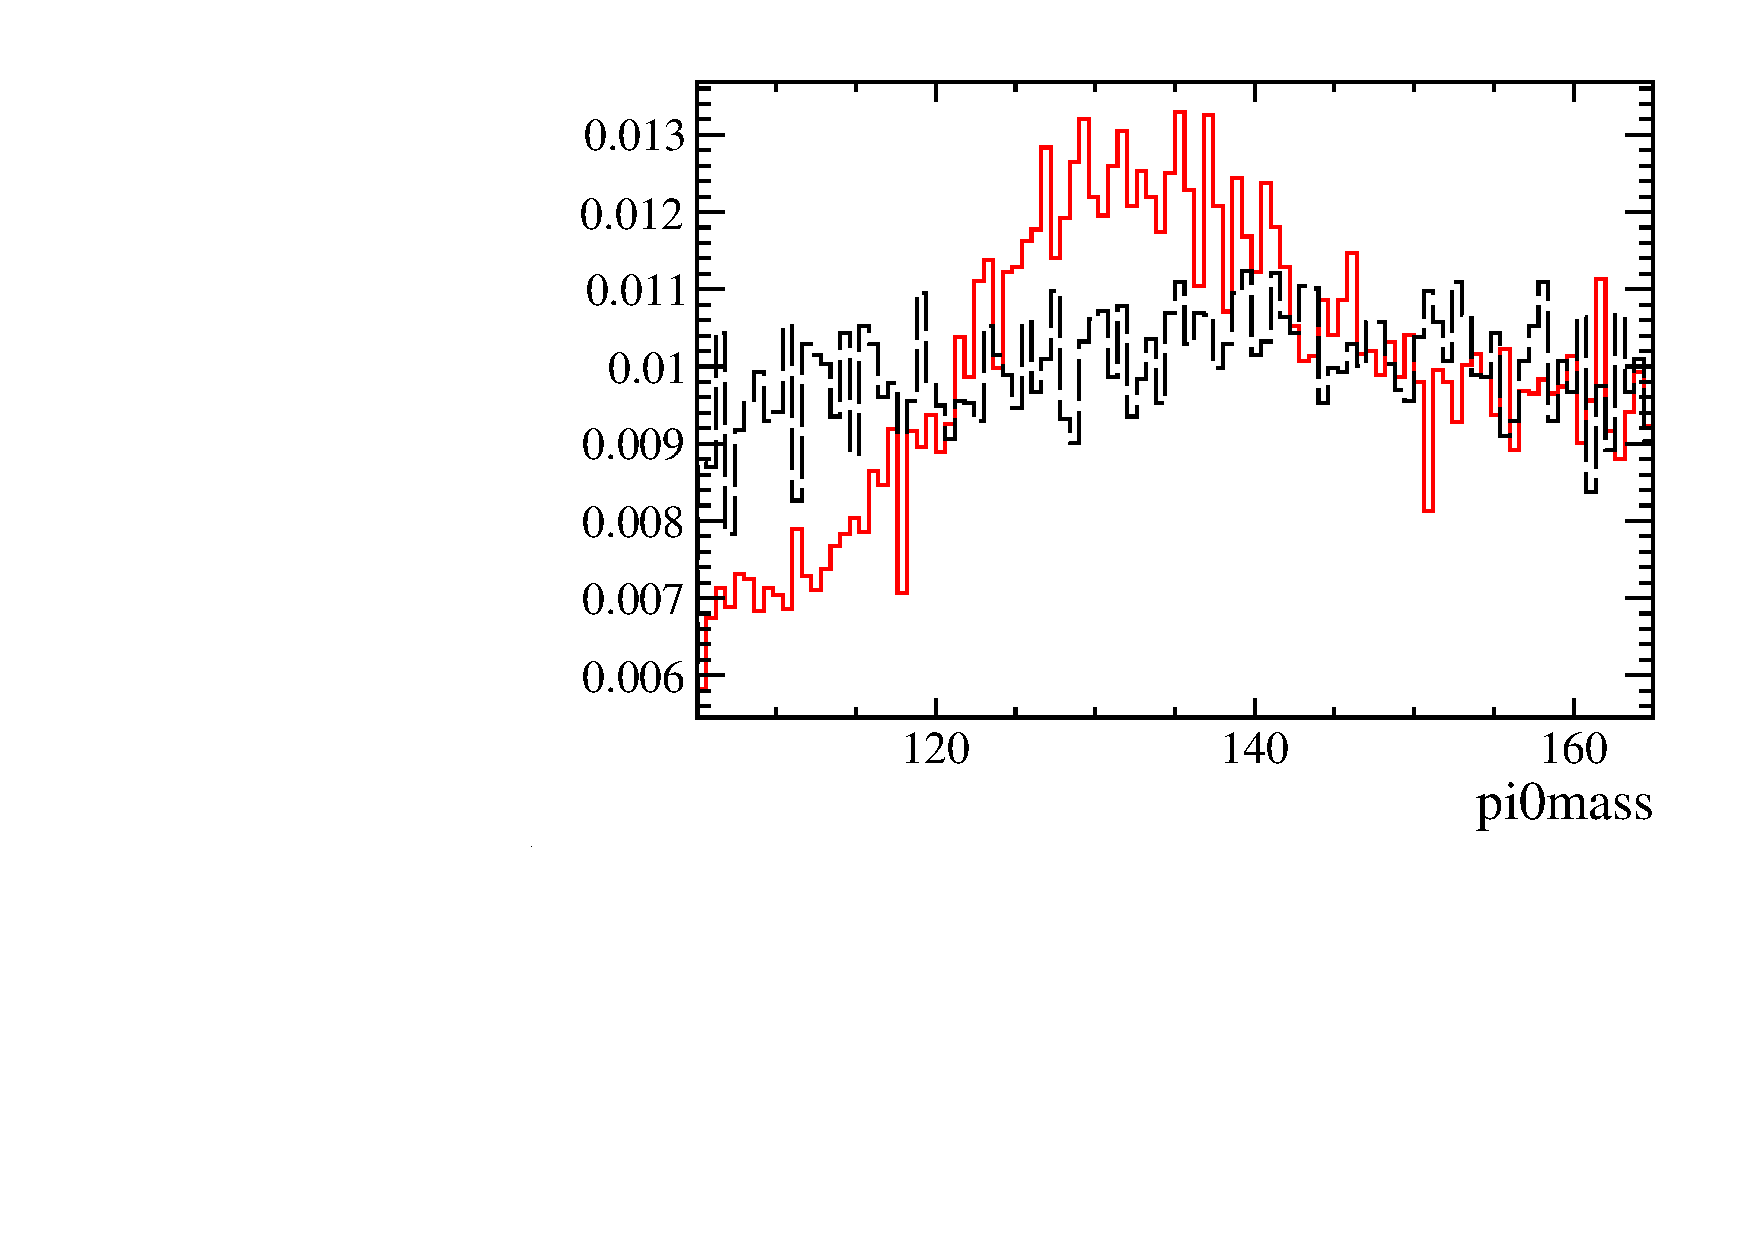
\includegraphics[scale=0.20]{figs/pi0massFULL.pdf}
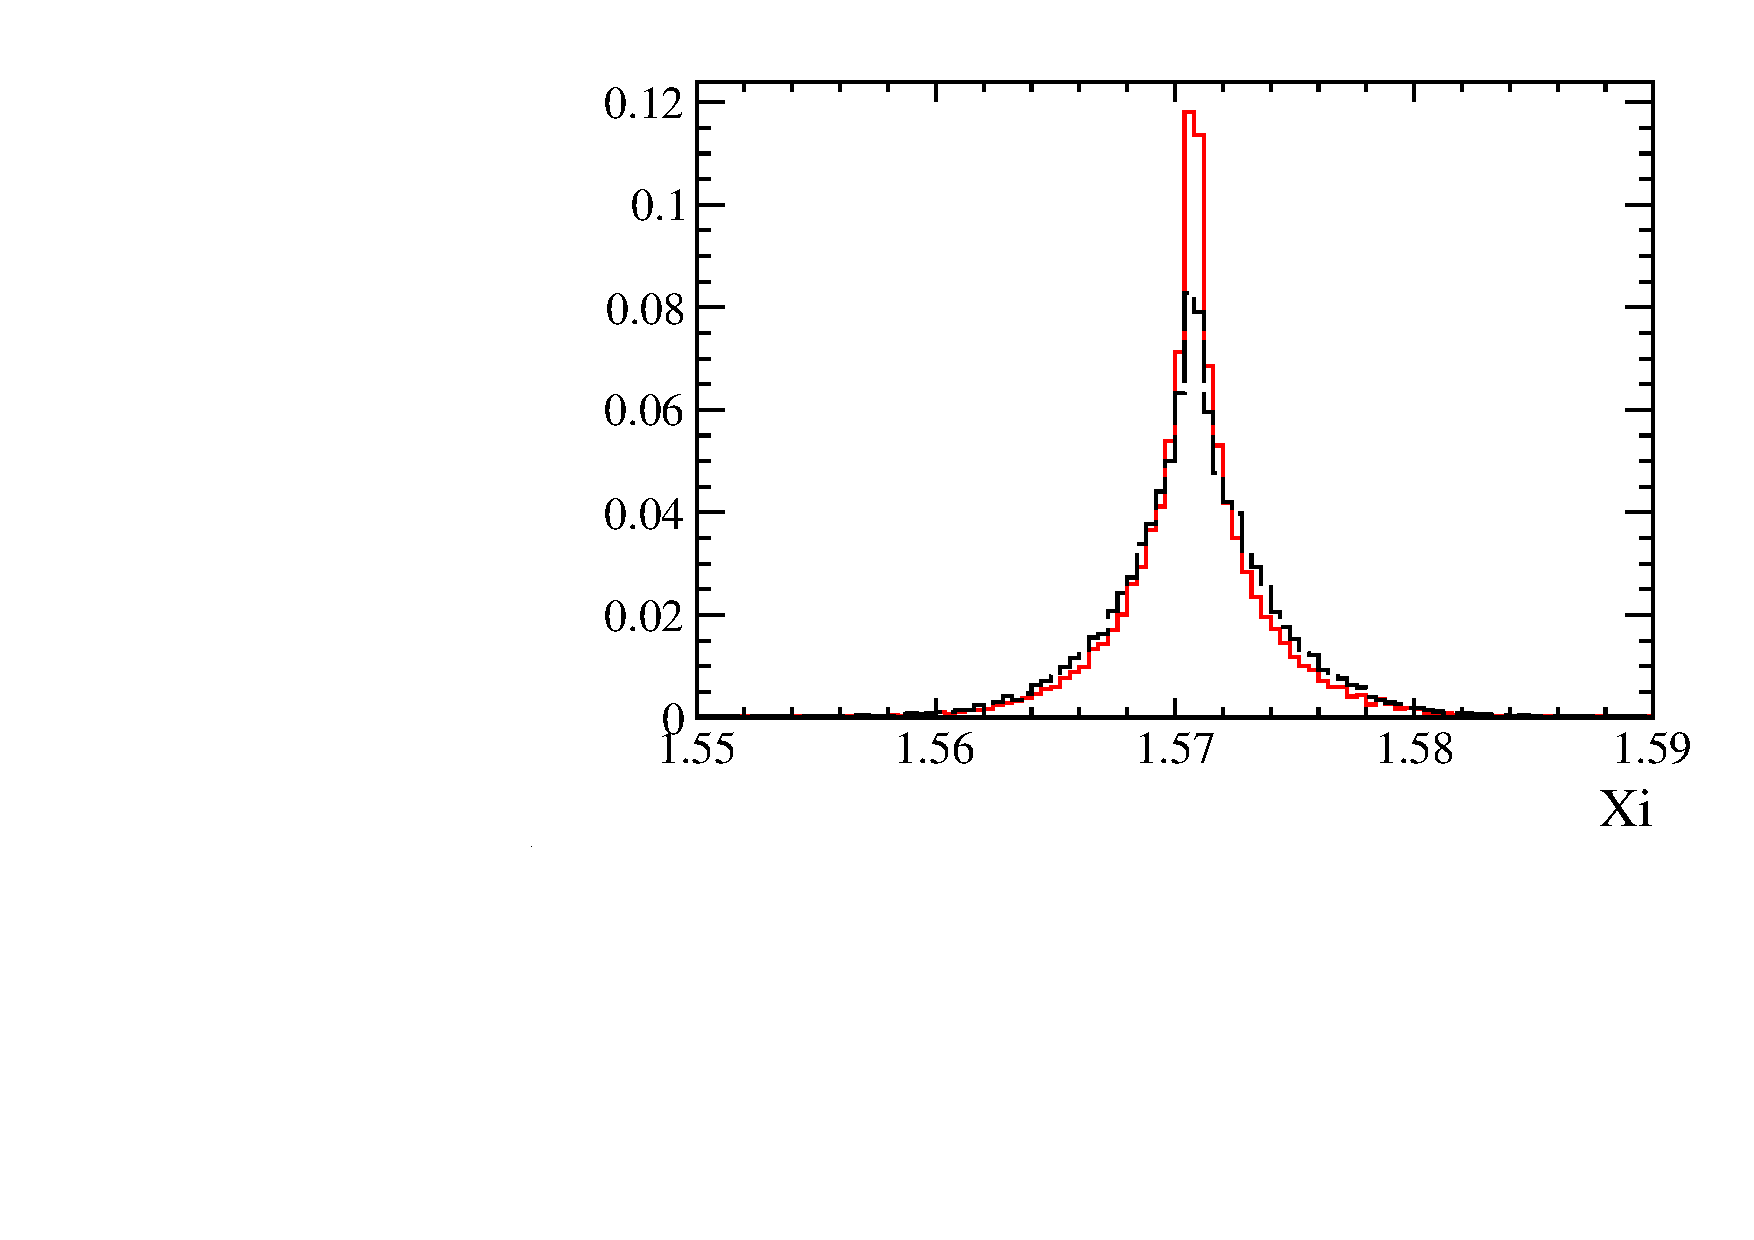
\includegraphics[scale=0.20]{figs/XiFULL.pdf}
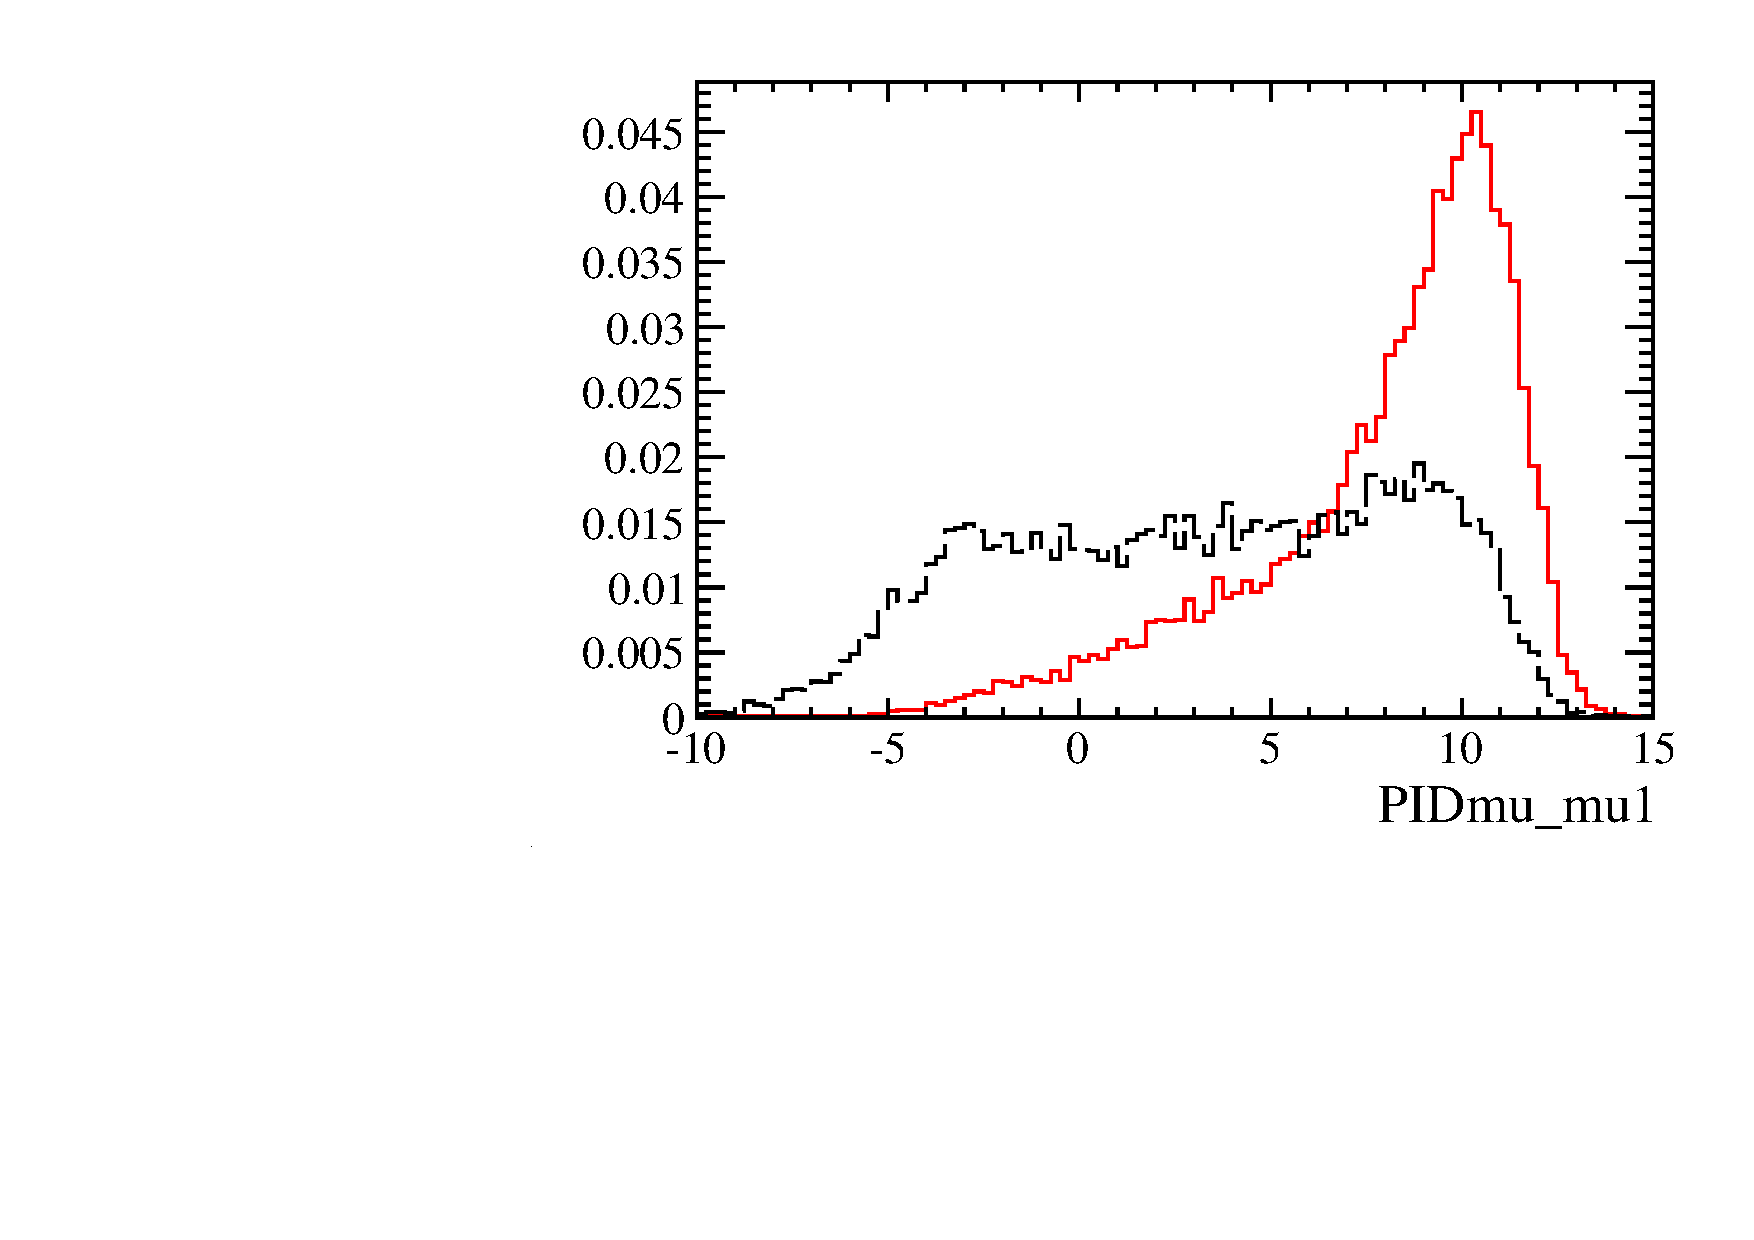
\includegraphics[scale=0.20]{figs/PIDmu_mu1FULL.pdf}
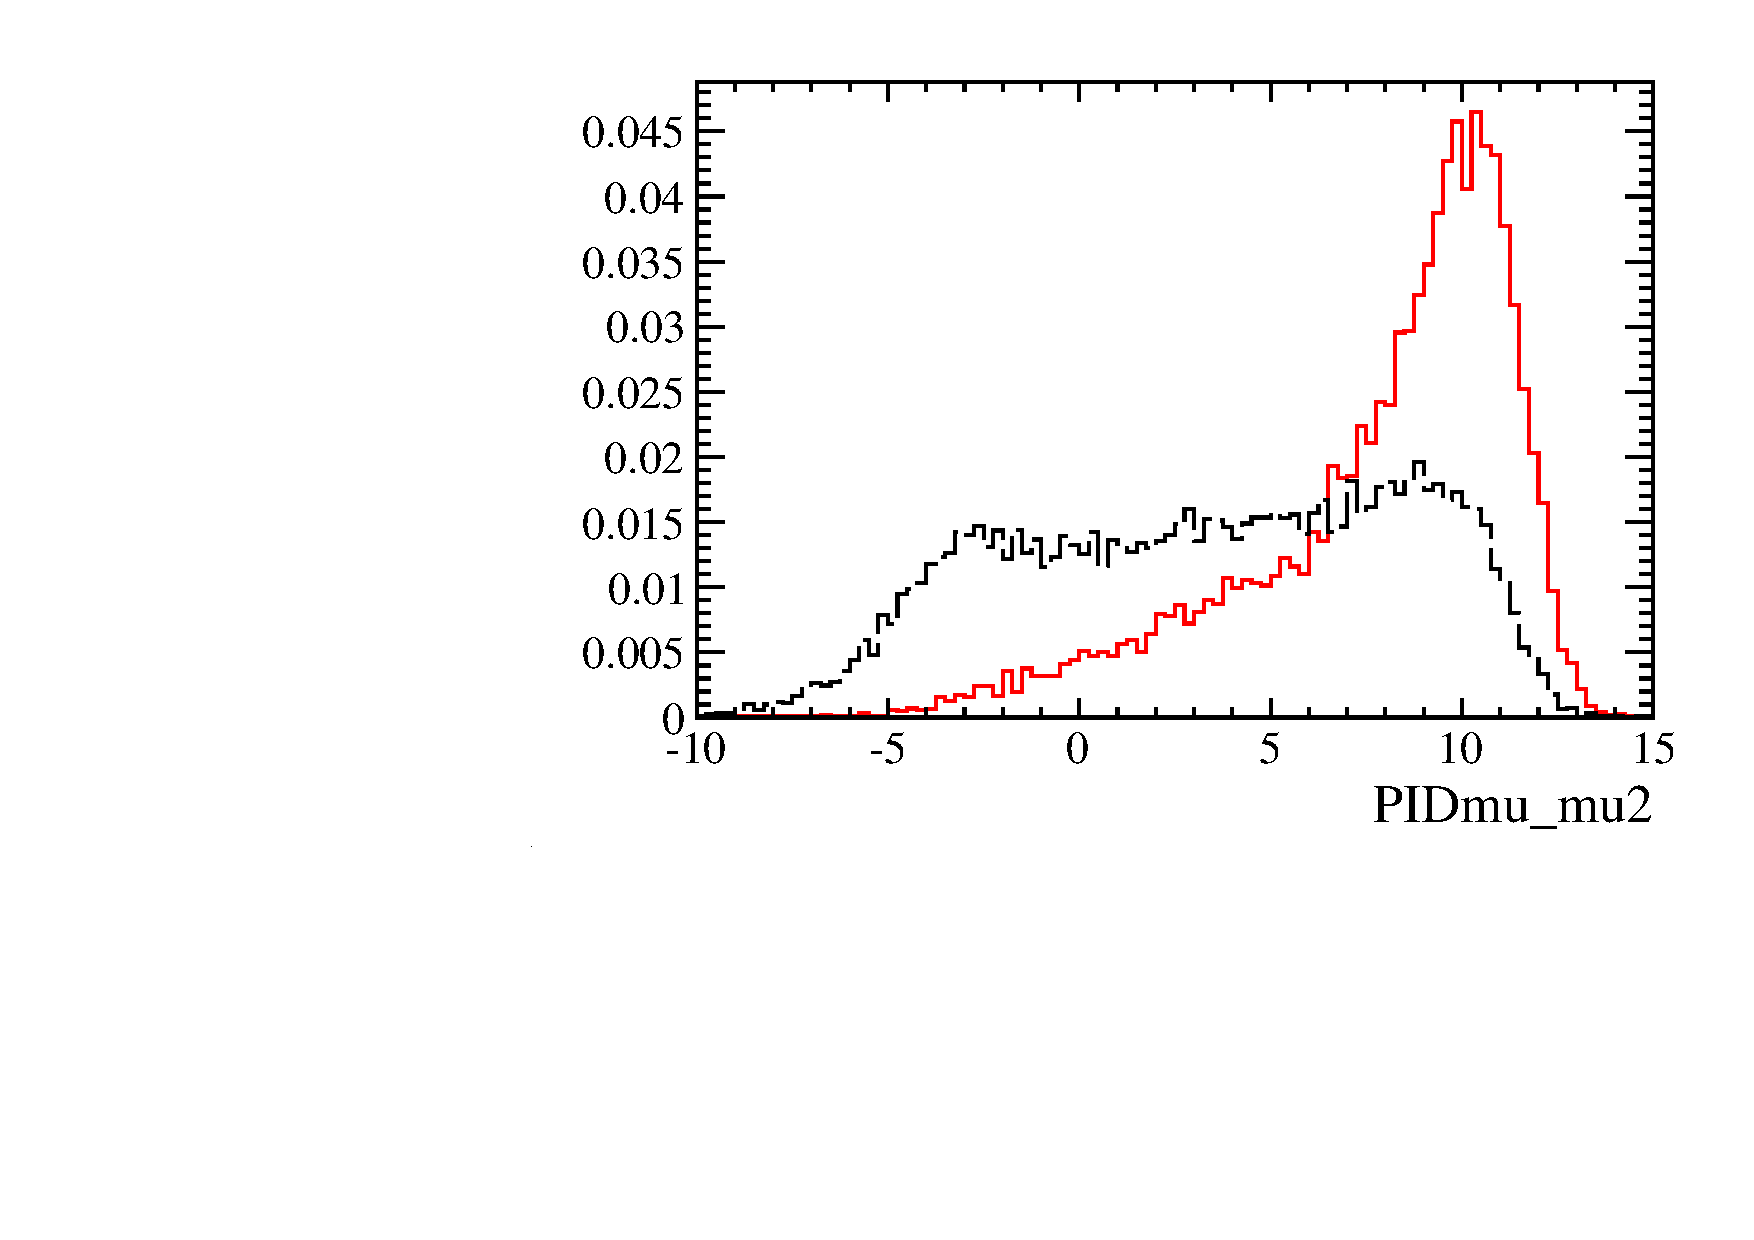
\includegraphics[scale=0.20]{figs/PIDmu_mu2FULL.pdf}
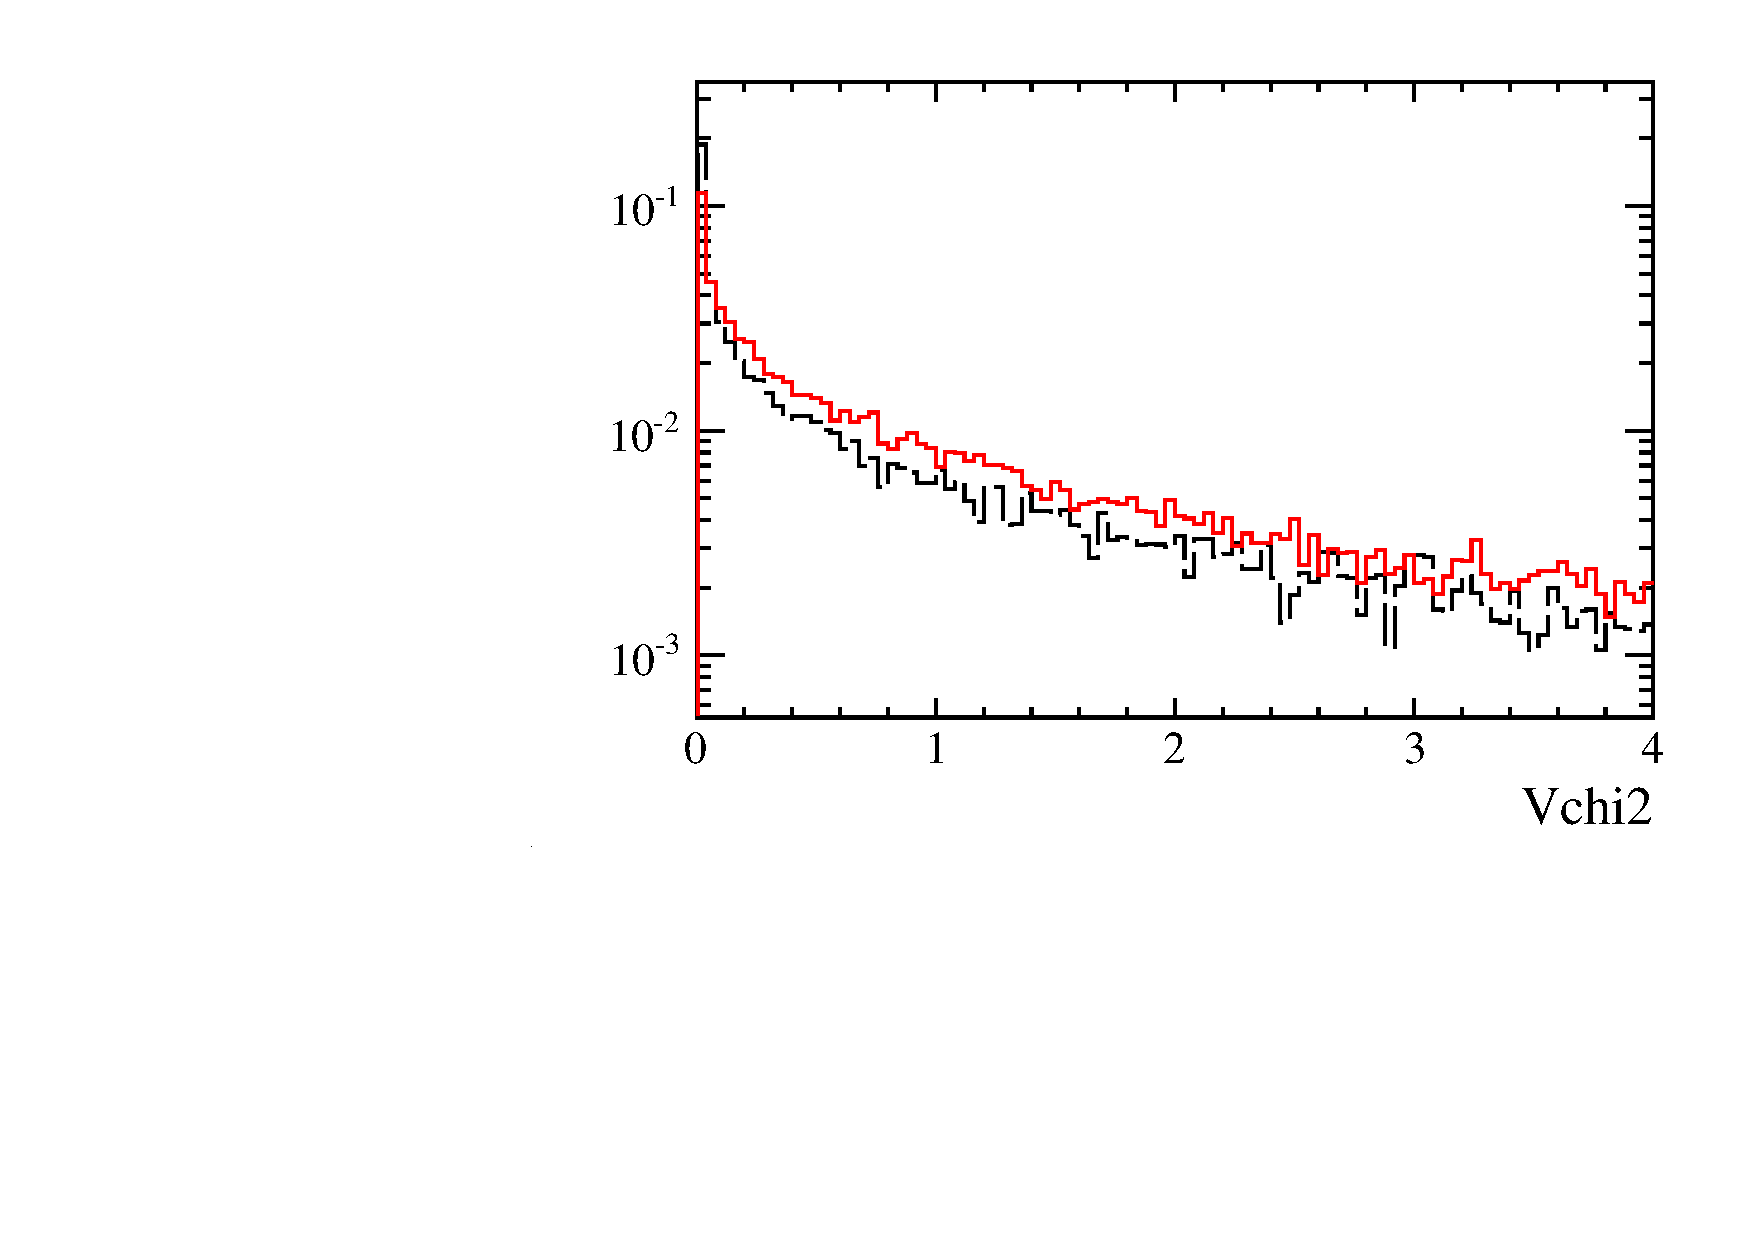
\includegraphics[scale=0.20]{figs/Vchi2FULL.pdf}
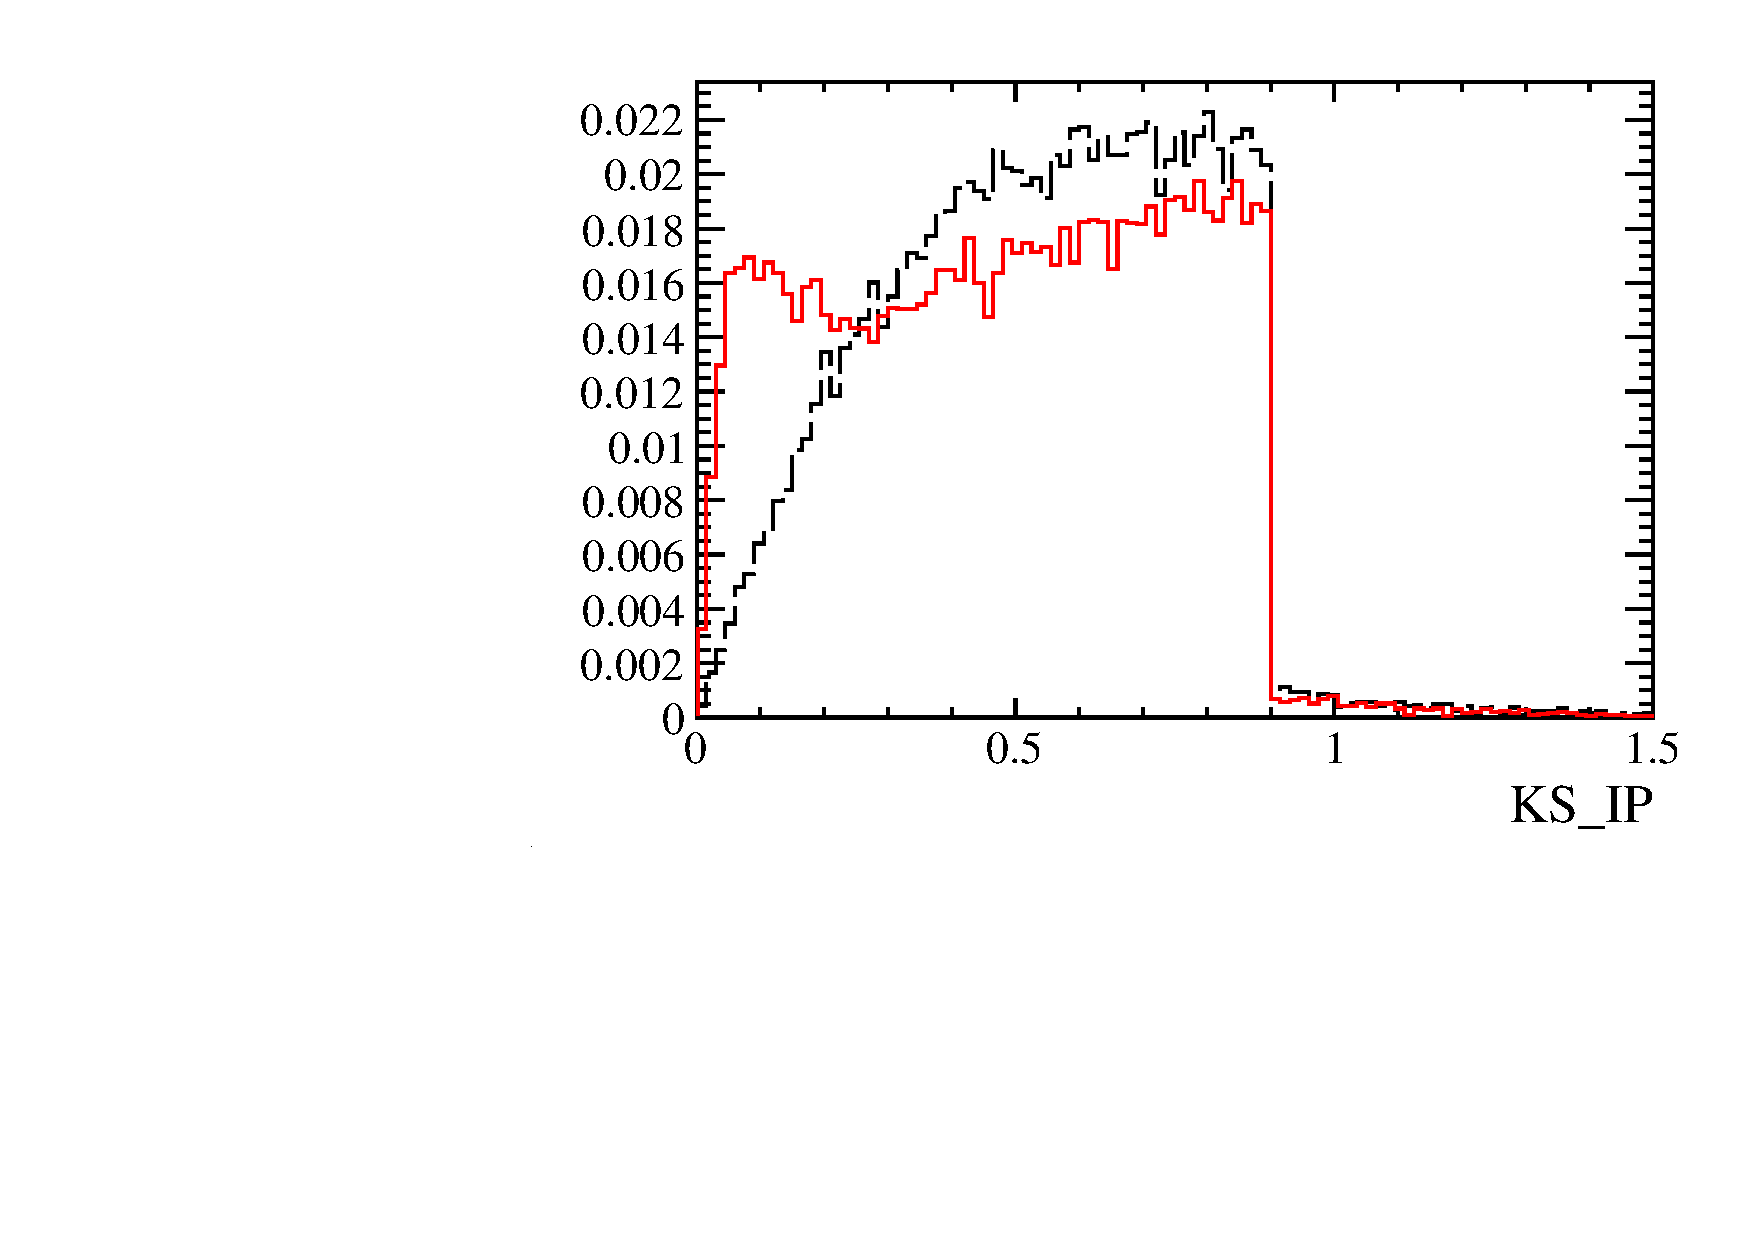
\includegraphics[scale=0.20]{figs/KS_IPFULL.pdf}
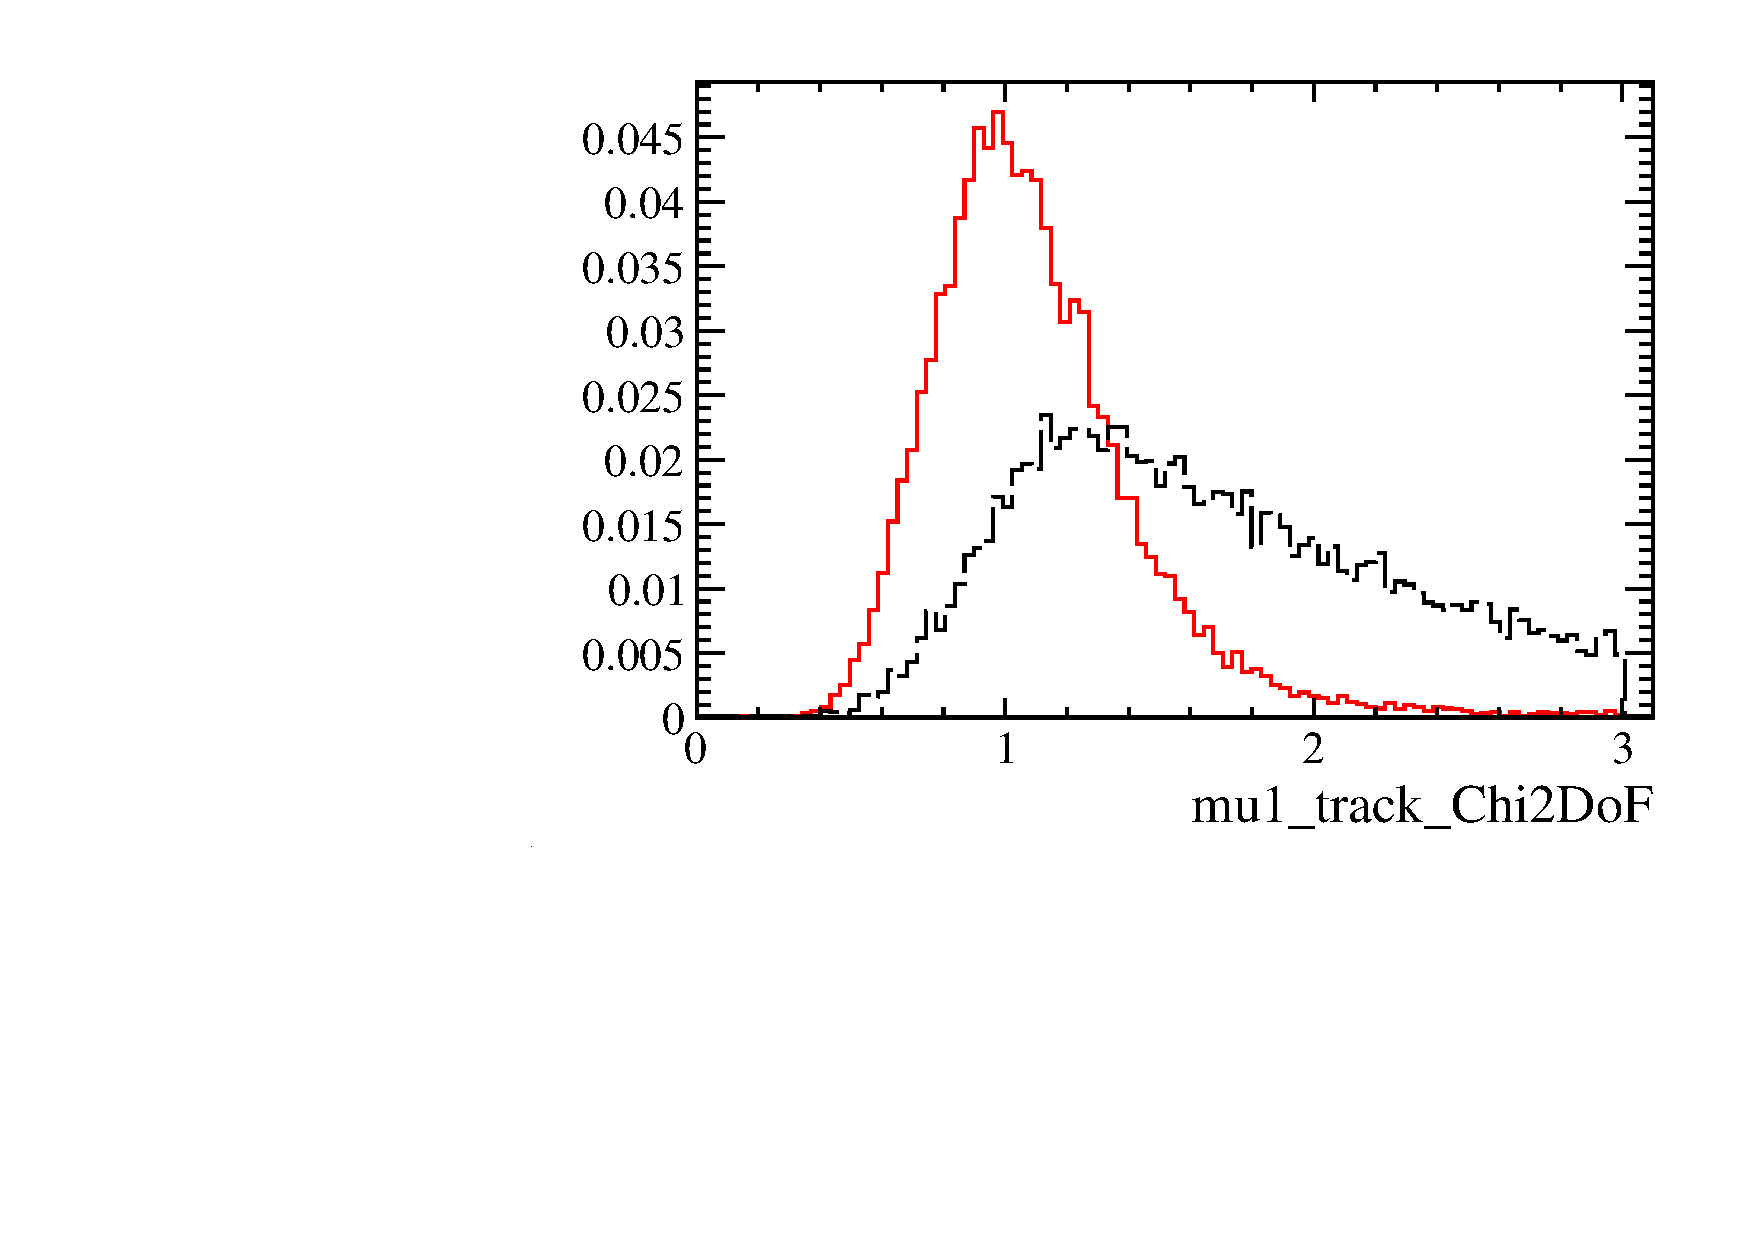
\includegraphics[scale=0.20]{figs/mu1_track_Chi2DoFFULL.pdf}
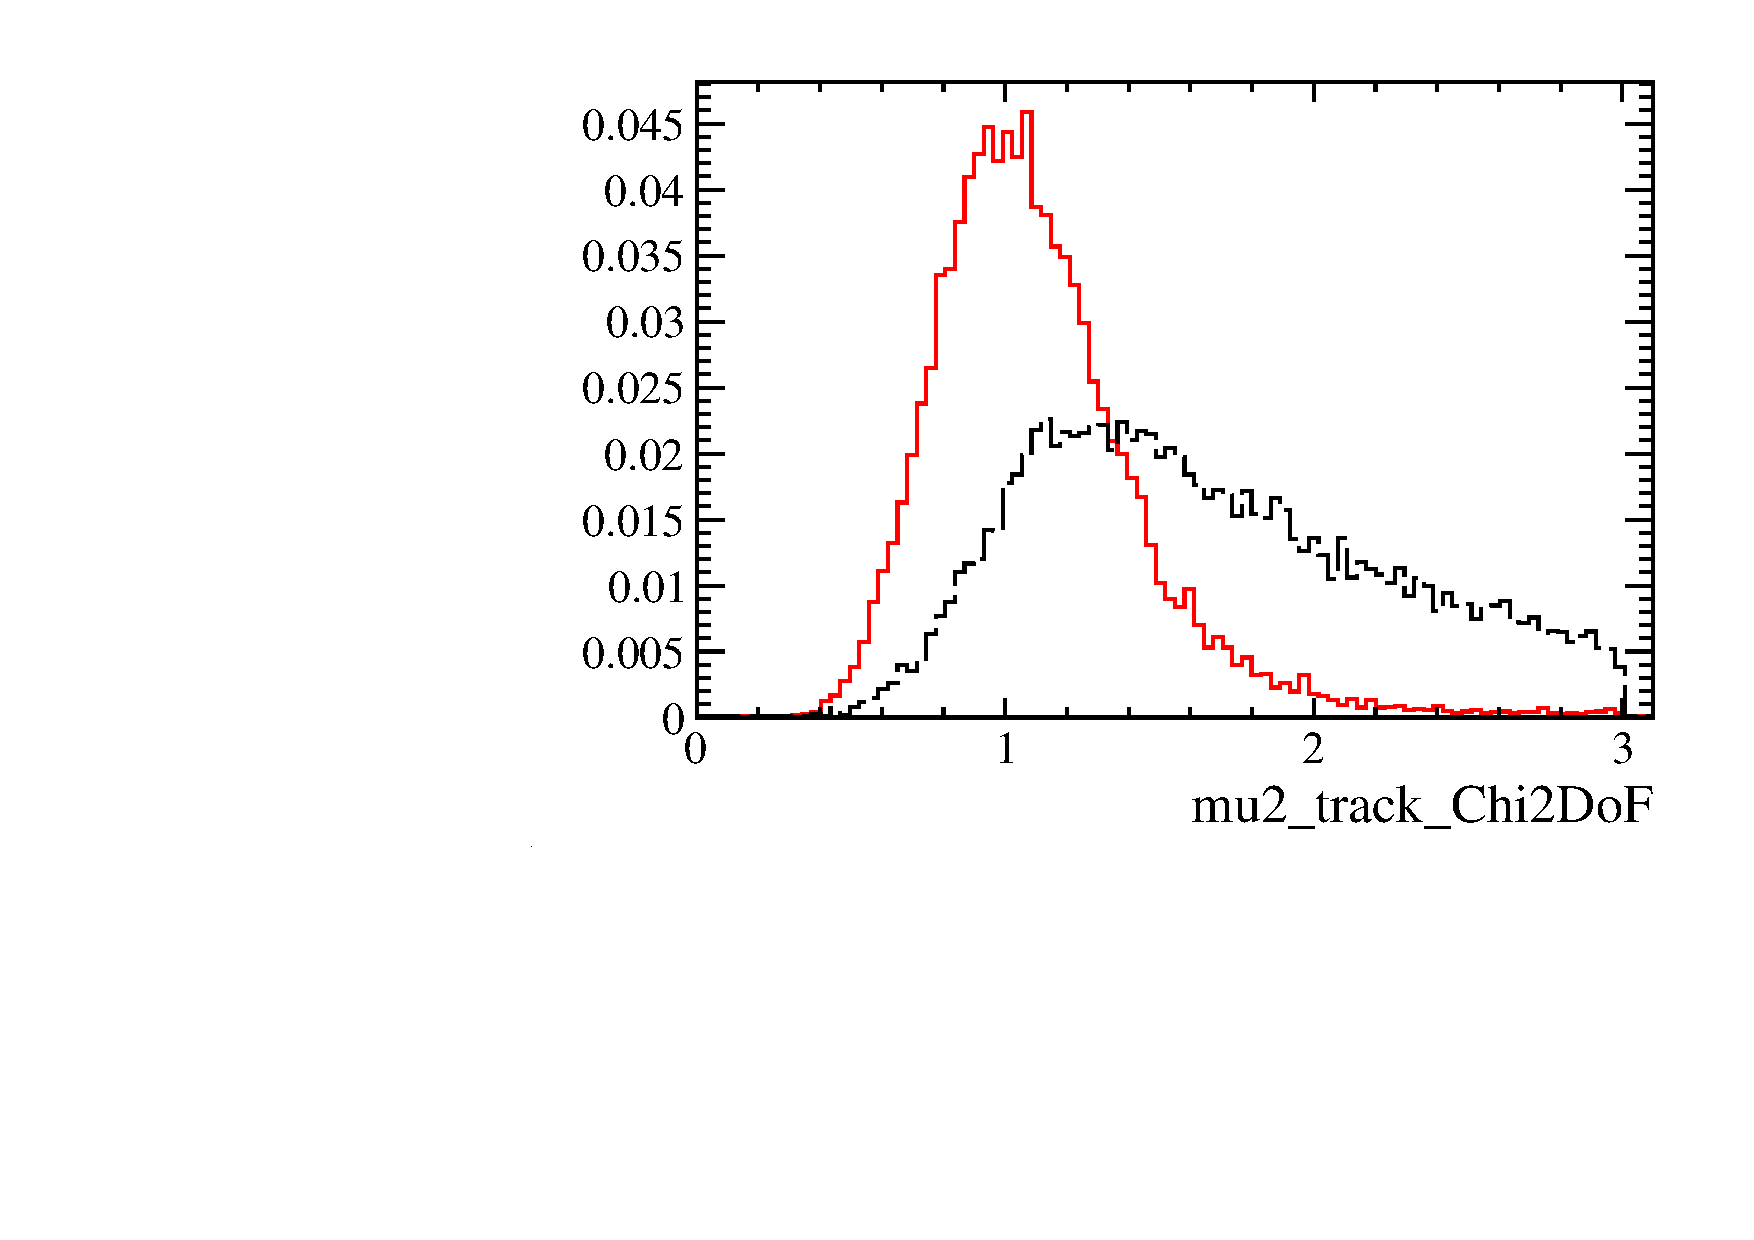
\includegraphics[scale=0.20]{figs/mu2_track_Chi2DoFFULL.pdf}
\includegraphics[scale=0.20]{figs/mu1_hitsInOTFULL.pdf}
\includegraphics[scale=0.20]{figs/mu2_hitsInOTFULL.pdf}
\includegraphics[scale=0.20]{figs/mu1_hitsInITFULL.pdf}
\includegraphics[scale=0.20]{figs/mu2_hitsInITFULL.pdf}
\includegraphics[scale=0.20]{figs/mu2_hitsInTTFULL.pdf}
\includegraphics[scale=0.20]{figs/mu1_hitsInTTFULL.pdf}
\caption{Input variable distributions for signal (red) and background (black) for the FULL case. \label{fig:MVAhistos_FULL1}}
\end{center}
\end{figure}

\begin{figure} [htb!]
\begin{center}
\includegraphics[scale=0.20]{figs/mu2_hitsInVFULL.pdf}
\includegraphics[scale=0.20]{figs/mu1_hitsInVFULL.pdf}
\includegraphics[scale=0.20]{figs/SV1FULL.pdf}
\includegraphics[scale=0.20]{figs/SV2FULL.pdf}
\includegraphics[scale=0.20]{figs/SV3FULL.pdf}
\caption{Input variable distributions for signal (red) and background (black) for the FULL case. \label{fig:MVAhistos_FULL2}}
\end{center}
\end{figure}

\begin{figure} [htb!]
\begin{center}
\includegraphics[scale=0.20]{figs/DOCAPARTIAL.pdf}
\includegraphics[scale=0.20]{figs/mu1ipsPARTIAL.pdf}
\includegraphics[scale=0.20]{figs/mu2ipsPARTIAL.pdf}
\includegraphics[scale=0.20]{figs/BipsPARTIAL.pdf}
\includegraphics[scale=0.20]{figs/BptPARTIAL.pdf}
\includegraphics[scale=0.20]{figs/BdissigPARTIAL.pdf}
\includegraphics[scale=0.20]{figs/PIDmu1PARTIAL.pdf}
\includegraphics[scale=0.20]{figs/PIDmu2PARTIAL.pdf}
\includegraphics[scale=0.20]{figs/Vchi2PARTIAL.pdf}
\includegraphics[scale=0.20]{figs/mu1_track_Chi2DoFPARTIAL.pdf}
\includegraphics[scale=0.20]{figs/mu2_track_Chi2DoFPARTIAL.pdf}
\includegraphics[scale=0.20]{figs/mu1_hitsInOTPARTIAL.pdf}
\includegraphics[scale=0.20]{figs/mu2_hitsInOTPARTIAL.pdf}
\includegraphics[scale=0.20]{figs/mu2_hitsInITPARTIAL.pdf}
\includegraphics[scale=0.20]{figs/mu1_hitsInITPARTIAL.pdf}
\includegraphics[scale=0.20]{figs/mu1_hitsInTTPARTIAL.pdf}
\includegraphics[scale=0.20]{figs/mu2_hitsInTTPARTIAL.pdf}
\includegraphics[scale=0.20]{figs/mu1_hitsInVPARTIAL.pdf}
\includegraphics[scale=0.20]{figs/mu2_hitsInVPARTIAL.pdf}
\includegraphics[scale=0.20]{figs/SV1PARTIAL.pdf}
\includegraphics[scale=0.20]{figs/SV2PARTIAL.pdf}
\includegraphics[scale=0.20]{figs/SV3PARTIAL.pdf}
\caption{Input variable distributions for signal (red) and background (black) for the PARTIAL case.
\label{fig:MVAhistos_PARTIAL}}
\end{center}
\end{figure}




%% $Id: introduction.tex 87303 2016-02-08 13:44:29Z lafferty $
\clearpage
\newpage
\section{Appendix: Samples used}
\label{sec:samples}
%{\it Miriam fill this}

The results described in this note were obtained using the data collected by LHCb at the LHC at a centre-of-mass energies of $\sqrt{s} = 7, 8 \text{ and } 13 \tev$ during the years 2011, 2012, and 2016, 
respectively. Both positive ($B_y > 0$) and negative ($B_y < 0$) magnet polarities are considered. 
%The data were reconstructed in the Reco14 framework using Brunel [7] v43r2p2, with
%the Condition Data Base [8] (condDB) tag cond-20121025 and the Detector Data Base [9]
%(DDDb) tag dddb-20120831. They were stripped with the Stripping20p3 reconstruction
%campaign, using DaVinci [10] v32r2p14.

Two separate stripping lines, described in \secref{app:selection}, are used for the FULL and PARTIAL categories. Note that in both cases that two different stripping lines are used for \Kspizmm and \Kspipi.
They are part of the LEPTONIC(MDST) stream for the Stripping 21 and DIMUON(DST) stream for the Stripping 24 and Stripping 26. \\
The following samples were used for the preparation of this note:
\begin{itemize}
\item Signal MC samples:
\begin{itemize}
%\item Event type 30000000, using the Sim08f configuration for the 2012 conditions. Reco14a framework, Stripping 20 NoPrescalingFlaggedALLSTREAMS
%\item Event type 34112401, using the Sim08c configuration for the 2012 conditions. Reco14a framework, Stripping 20 NoPrescalingFlaggedALLSTREAMS
\item Event type 34112407, using the Sim09a configuration for the 2012 conditions. Reco14c framework,condB tag~\cite{condDB} sim-20160321-2-vc-md100 (magnet down) and sim-20160321-2-vc-mu100 (magnet up), Detector Data base tag~\cite{dddb} dddb-20150928, Stripping 21 Filtered. %MC12
\item Event type 34102408, using the Sim09a configuration for the 2012 conditions. Reco14c framework,condB tag~\cite{condDB} sim-20160321-2-vc-md100 (magnet down) and sim-20160321-2-vc-mu100 (magnet up), Detector Data base tag~\cite{dddb} dddb-20150928, Stripping 21 Filtered. %MC12 bkg
\item Event type 34112407, using the Sim09a configuration for the 2015 conditions. Reco15a framework,condB tag~\cite{condDB} sim-20160606-vc-md100 (magnet down) and sim-20160606-vc-mu100 (magnet up), Detector Data base tag~\cite{dddb} dddb-20150724, Stripping 24 NoPrescalingFlagged. %MC15
%\item Event type 34112401, using the Sim08e configuration for the 2012 conditions. Reco14a framework, Stripping 20 NoPrescalingFlagged
\end{itemize}



%\begin{itemize}
%\item Stat,Generation Cuts, Stat to disk, Stat stripped (?)
%\end{itemize}
%Brunel ~\cite{brunel}
%condDB ~\cite{condDB}
%DDDb ~\cite{dddb}
%DaVinci ~\cite{DaVinci}
%Erasmus ~\cite{Erasmus}
\item Stripping 21 data.
\begin{itemize}
%\item Reco14 framework, Brunel~\cite{brunel} v43r2p2, condB tag~\cite{condDB} cond-20130114, Detector Data base tag~\cite{dddb} dddb-20130111. Stripping 21r1, DaVinci~\cite{DaVinci} v36r1. 
%Data from 2011 collisions, $0.992 \pm 0.001 \;\invfb$.
%\item Reco14 framework, Brunel~\cite{brunel} v43r2p2, condB tag~\cite{condDB} dddb-20120831, Detector Data base tag~\cite{dddb} dddb-20120831. Stripping 21, DaVinci~\cite{DaVinci} v36r1. 
%Data from 2012 collisions, $2.036 \pm 0.002 \;\invfb$.
\item Reco14 framework, Brunel~\cite{brunel} v43r2p2, condB tag~\cite{condDB} cond-20141107, Detector Data base tag~\cite{dddb} dddb-20130929. Stripping 21r1, DaVinci~\cite{DaVinci} v36r1. 
Data from 2011 collisions, $0.992 \pm 0.001 \;\invfb$.
\item Reco14 framework, Brunel~\cite{brunel} v43r2p2, condB tag~\cite{condDB} cond-20141107, Detector Data base tag~\cite{dddb} dddb-20130929-1. Stripping 21, DaVinci~\cite{DaVinci} v36r1. 
Data from 2012 collisions, $2.036 \pm 0.002 \;\invfb$.


\end{itemize}
% \item Stripping 24 data, 0.132 $fb^{-1}$.
% \begin{itemize}
% \item Reco15a framework, Brunel~\cite{brunel} v47r8, condB tag~\cite{condDB} cond-20150828, Detector Data base tag~\cite{dddb} dddb-20150724. Stripping 24, DaVinci~\cite{DaVinci} v38r1p1. Data from 2015 collisions.
% \end{itemize}
\item Stripping 26 data.
\begin{itemize}
\item Reco16 framework, Brunel~\cite{brunel} v47r8, condB tag~\cite{condDB} cond-20160522, Detector Data base tag~\cite{dddb} dddb-20150724. Stripping 26, DaVinci~\cite{DaVinci} v40r2p1. 
Data from 2016 collisions, $0.306 \pm 0.001 \;\invfb$.
\end{itemize}
\end{itemize}






%% $Id: introduction.tex 87303 2016-02-08 13:44:29Z lafferty $
\clearpage
\newpage
\section{Appendix: Normalization}
\label{app:normalization}

The signal yield is normalised with respect to \Kspipi . The yield is computed as follows:
\begin{equation}
N(\KsPzMuMu) = \sigma(\PKzS){\cal B}(\KsPzMuMu)\epsilon_{\KsPzMuMu} L,
\end{equation}
where $\sigma(\PKzS)$ is the \KS production cross-section, $\epsilon_{\KsPzMuMu}$ the absolute efficiency and $L$ the integrated luminosity. Taking the ratio of N(\KsPzMuMu) with respect to N(\Kspipi), both the 
cross-section and the luminosity get cancelled out, leading to the formula:

\begin{equation}
\frac{N(\KsPzMuMu)}{N(\Kspipi)} = \frac{\BRof\KsPzMuMu}{\BRof\Kspipi} \frac{\epsilon_{\KsPzMuMu}}{\epsilon_{\PKzS\to\Pgpp\Pgpm}}.
\end{equation}

The effective luminosity, $L^{dat}_{eff}$, is calculated according to

\begin{equation}
L^{dat}_{eff} = \epsilon^{TIS}_{\Kspipi}L^{dat}, \\
\end{equation}	
where $\epsilon_{TIS}(\Kspipi)$ is the TIS efficiency calulated using \Kspipi events and $L^{dat}$ is the luminosity used for the fit to the data.

\begin{eqnarray}
L^{FULL,2011}_{eff} &=& 0.0016 \cdot 992\;\rm pb^{-1} = 1.59\;\invpb, \\
L^{FULL,2012}_{eff} &=& 0.0016 \cdot 2037\;\rm pb^{-1} = 3.26\;\invpb,\\
L^{PARTIAL}_{eff} &=& 0.0025 \cdot 306\;\rm pb^{-1} = 0.77\;\invpb. 
\end{eqnarray}

The offline signal efficiency (or, equivalently, the total efficiency for a $100\%$ efficient trigger) for the FULL channel is calculated as follows:
\begin{itemize}

\item The generator level efficiency is estimated to be $0.361$. 
\item The efficiency of the FULL stripping on generated events is $1.84$ per mil according to the statistics produced by the DaVinci filtering script. This number has to be corrected by the fact that $3.3\%$ of the events didn't actually contain a signal candidate at all \footnote{In a fraction of events, the information on how the \KS should decay is lost as the particle is passed to GEANT4.}. It also has to be corrected by the fact that some of the selected candidates aren't matched to the signal. After this corrections, it becomes $1.79$ per mil.
\item The efficiency of the fiducial cuts  and mass fit window are $0.931$ and $0.922$. These are applied prior to BDT training.
\end{itemize}

The offline signal efficiency (or, equivalently, the total efficiency for a $100\%$ efficient trigger) for the PARTIAL channel is calculated as follows:
\begin{itemize}

\item The generator level efficiency is estimated to be $0.361$. 
\item The efficiency of the PARTIAL stripping on generated events, calculated in the same way as above is $1.23\%$.
\item The efficiency of the fiducial cuts  and mass fit window are $0.734$ and $0.917$ respectively. These are applied prior to BDT training.
\end{itemize}

%% $Id: introduction.tex 87303 2016-02-08 13:44:29Z lafferty $
\clearpage
\newpage

\section{Appendix: Peaking background studies}
\label{app:background}

%{\it Give details on the \KL supression factor and on the \KLTpi}

The upper decay time acceptance (mainly the limited size of the VELO) causes the \KL reconstruction efficiency to be much lower than that of the \KS by about a factor of thousand ~\cite{KsmmANA}. We checked that a similar 
factor applies to our decay. Indeed, repeating the calculations of Sect.~6 in Ref.~\cite{KsmmANA} using our measured value of $\alpha_{\Kspizmm} = -110.9\pm 1.2 \; \rm ns^{-1}$ (see \figref{fig:lifetime}), we recovered an efficiency 
ratio factor of $\approx 2.2\times10^{-3}$.

\begin{figure} [htb!]
\begin{center}
\includegraphics[scale=0.3]{figs/lifetime.pdf}
%\includegraphics[scale=0.30]{figs/mK3pi_PARTIAL_wKsPiPi.pdf}
\caption{Lifetime distribution of selected \Kspizmm for $t>8.95\;\rm ps$. The red line shows an exponential fit, used to obtain $\alpha$~\cite{KsmmANA}. \label{fig:lifetime}}
\end{center}
\end{figure}


Samples of $K^0_S\rightarrow\pi^+\pi^-\pi^0$ corresponding to event type 34102408 were generated in order to study the \KLTpi  background.
The invariant mass distribution of the events stripped in a sample of $K^0_S\rightarrow\pi^+\pi^-\pi^0$ is shown in \figref{fig:KLTpi_wKspipi}. 
It can be seen as the right hand side bump (see also \figref{fig:mumuKspipi}) where we also included the \Kspipi from the underlying event and that also pass the selection. 
The Ismuon requirement was dropped from the stripping to increase the statistics. We find 254 \Kspipi out of 735 candidates. Taking into account the suppresion factor for \KL to \KS ($\sim2\times10^{-3}$), 
the MC generation efficiency ($\approx 0.36$) and the fact that the $3\pi$ decays is forced, we expect a ratio of $\sim2\times10^{-4}$ \KLTpi per \Kspipi decay in our PARTIAL background. 
A stripping 21 (i.e, FULL) filtered \KSTpi sample is also available. In that case we find about $50\%$  of the events actually come from the forced decay. Again, taking into account the \KL to \KS supression factor, 
we find that this background is small compared to other sources. The BDT and mass distributions of the 18 events of the filtered sample which also pass the selection cuts applied prior to BDT training is shown in 
\figref{fig:KLTpi_BDT}. No events are in the BDT region used for the fit, and the effective luminosity of the sample is insufficient to derive a meaningful quantitative upper limit on the number of \KLTpi events expected 
in the data. Finally, in order to asess the possible impact on the sensitivity, we add to the fit a Landau component with parameters fixed to those obtained from simulation at the stripping filtered level (we lack 
statistics to do it after all cuts and per BDT bin), as shown in \figref{fig:Landau}. The fit to data is shown in \figref{fig:fitK3pi}. The expected sensitivity for 50 fb$^{-1}$ including this component is 
$\pm5.3\times10^{-9}$, very similar to the one obtained when this component is ignored, $5.5\times10^{-9}$. The size of the Landau component is consistent with zero at one sigma in all BDT bins.


   
To study the contribution of a background due to three-pion final state decays, such as $\eta\to\pi^+\pi^-\pi^0$, the invariant $K^{0}$ mass is reconstructed using the pion mass hypothesis
for the muons. The corresponding distributions are shown in \figref{fig:eta_bkg}. No peaking structures in the signal region are to be seen.
   
\begin{figure} [htb!]
\begin{center}
\includegraphics[scale=0.60]{figs/M_V0_K3pi_Kspipi.pdf}%{figs/mK3pi_PARTIAL_wKsPiPi.pdf}
%\includegraphics[scale=0.30]{figs/mK3pi_PARTIAL_wKsPiPi.pdf}
\caption{Invariant mass distribution of simulated $K^0\rightarrow\pi^+\pi^-\pi^0$ decays selected in the PARTIAL category including also the \Kspipi decays that got selected from the underlying event, 
which can be seen as the right hand side bump. \label{fig:KLTpi_wKspipi}}
\end{center}
\end{figure}
   
\begin{figure} [htb!]
\begin{center}
\includegraphics[scale=0.60]{figs/M_mumu_K3pi_Kspipi.pdf}%{figs/mumu_mass.pdf}
%\includegraphics[scale=0.30]{figs/mumu_mass.pdf}
\caption{Invariant mass distribution of dimuon candidates in simulated $K^0\rightarrow\pi^+\pi^-\pi^0$ decays selected in the PARTIAL category, and including also the \Kspipi that got selected from the underlying event. 
\label{fig:mumuKspipi}}
\end{center}
\end{figure}

\begin{figure} [htb!]
\begin{center}
\includegraphics[scale=0.3]{figs/filtered_mass_BDTintegrated.pdf}
\includegraphics[scale=0.30]{figs/K3pi_BDT.pdf}
\caption{Mass and BDT distribution of the \KSTpi simulated FULL candidates.\label{fig:KLTpi_BDT}}
\end{center}
\end{figure}
\begin{figure} [htb!]
\begin{center}
\includegraphics[scale=0.6]{figs/landau.pdf}
\caption{Mass of \KSTpi after stripping FULL, and fit to a Landau \pdf. \label{fig:Landau}}
\end{center}
\end{figure}

\begin{figure} [htb!]
\begin{center}
\includegraphics[scale=0.5]{figs/fit_wK3pi.pdf}
%\includegraphics[scale=0.30]{figs/K3pi_BDT.pdf}
\caption{Fit to the dataset FULL including a Landau component for \KLTpi. The size of the Landau component is consistent with zero at one sigma in all BDT bins. \label{fig:fitK3pi}}
\end{center}
\end{figure}


\begin{figure} [htb!]
\begin{center}
\includegraphics[scale=0.30]{figs/M_VC_pipi_hyp.pdf}
\includegraphics[scale=0.30]{figs/M_V0_pipi_hyp.pdf}
\caption{Invariant $\pi^{+}\pi^{-}\pi^0$ mass distribution of kaon candidates in decays in the FULL (left) and PARTIAL (right) data samples. The kaon mass is reconstructed using the pion mass hypothesis for the muons. \label{fig:eta_bkg}}
\end{center}
\end{figure}




%\section{Detector and simulation}
\label{sec:Detector}
The paragraph below can be used for the detector
description. Modifications may be required in specific papers to fit
within page limits, to enhance particular detector elements or to
introduce acronyms used later in the text. For journals where strict
word counts are applied (for example, PRL), and space is at a premium,
it may be sufficient to write, as a minimum: ``The LHCb detector is a 
single-arm forward spectrometer covering the pseudorapidity range 
$2 < \eta < 5$, 
described in detail in Refs.~\cite{Alves:2008zz,LHCb-DP-2014-002}''. 
A slightly longer version could specify the most relevant sub-detectors, {\it e.g} 
``The LHCb 
detector~\cite{Alves:2008zz,LHCb-DP-2014-002} is a
single-arm forward spectrometer covering the pseudorapidity range $2 < \eta < 5$, designed for
the study of particles containing b or c quarks. The detector elements that are particularly
relevant to this analysis are: a silicon-strip vertex detector surrounding the pp interaction
region that allows c- and b-hadrons to be identified from their characteristically long
flight distance; a tracking system that provides a measurement of momentum, $p$, of charged
particles; and two ring-imaging Cherenkov detectors that are able to discriminate between
different species of charged hadrons.'' 

\begin{verbatim}
In the following paragraph, references to the individual detector 
performance papers are marked with a * and should only be included 
if the analysis relies on numbers or methods described in the specific 
papers. Otherwise, a reference to the overall detector performance 
paper~\cite{LHCb-DP-2014-002} will suffice. Note also that the text 
defines the acronyms for primary vertex, PV, and impact parameter, IP. 
Remove either of those in case it is not used later on.
\end{verbatim}

The \lhcb detector~\cite{Alves:2008zz,LHCb-DP-2014-002} is a single-arm forward
spectrometer covering the \mbox{pseudorapidity} range $2<\eta <5$,
designed for the study of particles containing \bquark or \cquark
quarks. The detector includes a high-precision tracking system
consisting of a silicon-strip vertex detector surrounding the $pp$
interaction region~\cite{LHCb-DP-2014-001}\verb!*!, a large-area silicon-strip detector located
upstream of a dipole magnet with a bending power of about
$4{\mathrm{\,Tm}}$, and three stations of silicon-strip detectors and straw
drift tubes~\cite{LHCb-DP-2013-003}\verb!*! placed downstream of the magnet.
The tracking system provides a measurement of momentum, \ptot, of charged particles with
a relative uncertainty that varies from 0.5\% at low momentum to 1.0\% at 200\gevc.
The minimum distance of a track to a primary vertex (PV), the impact parameter (IP), 
is measured with a resolution of $(15+29/\pt)\mum$,
where \pt is the component of the momentum transverse to the beam, in\,\gevc.
Different types of charged hadrons are distinguished using information
from two ring-imaging Cherenkov detectors~\cite{LHCb-DP-2012-003}\verb!*!. 
Photons, electrons and hadrons are identified by a calorimeter system consisting of
scintillating-pad and preshower detectors, an electromagnetic
calorimeter and a hadronic calorimeter. Muons are identified by a
system composed of alternating layers of iron and multiwire
proportional chambers~\cite{LHCb-DP-2012-002}\verb!*!.
The online event selection is performed by a trigger~\cite{LHCb-DP-2012-004}\verb!*!, 
which consists of a hardware stage, based on information from the calorimeter and muon
systems, followed by a software stage, which applies a full event
reconstruction.

A more detailed description of the 'full event reconstruction' could be:
\begin{itemize}
\item The trigger~\cite{LHCb-DP-2012-004}\verb!*! consists of a
hardware stage, based on information from the calorimeter and muon
systems, followed by a software stage, in which all charged particles
with $\pt>500\,(300)\mev$ are reconstructed for 2011\,(2012) data.
For triggers that require neutral particles, 
energy deposits in the electromagnetic calorimeter are 
analysed to reconstruct \piz and $\gamma$ candidates.
\end{itemize}

The trigger description has to be specific for the analysis in
question. In general, you should not attempt to describe the full
trigger system. Below are a few variations that inspiration can be
taken from. First from a hadronic analysis, and second from an
analysis with muons in the final state.
A detailed description of the trigger conditions for Run 1 is available in
Ref.~\cite{LHCb-PUB-2014-046}.


\begin{itemize}
\item At the hardware trigger stage, events are required to have a muon with high \pt or a
  hadron, photon or electron with high transverse energy in the calorimeters. For hadrons,
  the transverse energy threshold is 3.5\gev.
  The software trigger requires a two-, three- or four-track
  secondary vertex with a significant displacement from the primary
  $pp$ interaction vertices. At least one charged particle
  must have a transverse momentum $\pt > 1.7\gevc$ and be
  inconsistent with originating from a PV.
  A multivariate algorithm~\cite{BBDT} is used for
  the identification of secondary vertices consistent with the decay
  of a \bquark hadron.
%\item The software trigger requires a two-, three- or four-track
%  secondary vertex with a large sum of the transverse momentum, \pt, of
%  the tracks and a significant displacement from the primary $pp$
%  interaction vertices~(PVs). At least one track should have $\pt >
%  1.7\gevc$ and \chisqip with respect to any
%  primary interaction greater than 16, where \chisqip is defined as the
%  difference in \chisq of a given PV reconstructed with and
%  without the considered track.\footnote{If this sentence is used to define \chisqip
%  for a composite particle instead of for a single track, replace ``track'' by ``particle'' or ``candidate''}
% A multivariate algorithm~\cite{BBDT} is used for
%  the identification of secondary vertices consistent with the decay
%  of a \bquark hadron.
\item The $\decay{\Bd}{\Kstarz\mumu}$ signal candidates are first required
      to pass the hardware trigger, which selects events containing at least
      one muon with transverse momentum $\pt>1.48\gevc$ in the 7\tev data or
      $\pt>1.76\gevc$ in the 8\tev data.  In the subsequent software
      trigger, at least one of the final-state particles is required to 
      have $\pt>1.7\gevc$ in the 7\tev data or $\pt>1.6\gevc$ in the 8\tev 
      data, unless the particle is identified as a muon in which case 
      $\pt>1.0\gevc$ is required. The final-state particles that 
      satisfy these transverse momentum criteria are also required 
      to have an impact parameter larger than $100\mum$ with respect 
      to all PVs in the event. Finally, the tracks of two or more of 
      the final-state particles are required to form a vertex that is 
      significantly displaced from the PVs." 

%  Candidate events are first required to pass the hardware trigger,
%  which selects muons with a transverse momentum $\pt>1.48\gevc$ 
%  in the 7\tev data or $\pt>1.76\gevc$ in the 8\tev data.
%  In the subsequent software trigger, at least
%  one of the final-state particles is required to have both
%  $\pt>0.8\gevc$ and impact parameter larger than $100\mum$ with respect to all
%  of the primary $pp$ interaction vertices~(PVs) in the
%  event. Finally, the tracks of two or more of the final-state
%  particles are required to form a vertex that is significantly
%  displaced from the PVs.
\end{itemize}

An example to describe the use of both TOS and TIS events:
\begin{itemize}
\item In the offline selection, trigger signals are associated with reconstructed particles.
%Selection requirements can therefore be made not only on the trigger requirement,
%but on whether the decision was due to the signal candidate, other particles produced in the $pp$ collision, or a combination of both.
Selection requirements can therefore be made on the trigger selection itself
and on whether the decision was due to the signal candidate, other particles produced in the $pp$ collision, or a combination of both.
\end{itemize}

A good example of a description of long and downstream \KS is given in 
Ref.~\cite{LHCb-PAPER-2014-006}:
\begin{itemize}
\item
Decays of \decay{\KS}{\pip\pim} are reconstructed in two different categories:
the first involving \KS mesons that decay early enough for the
daughter pions to be reconstructed in the vertex detector; and the
second containing \KS that decay later such that track segments of the
pions cannot be formed in the vertex detector. These categories are
referred to as \emph{long} and \emph{downstream}, respectively. The
long category has better mass, momentum and vertex resolution than the
downstream category.
\end{itemize}

The description of our software stack for simulation is often
causing trouble. The following paragraph can act as inspiration but
with variations according to the level of detail required and if
mentioning of \eg \photos is required.
\begin{itemize}
\item In the simulation, $pp$ collisions are generated using
\pythia~\cite{Sjostrand:2006za,*Sjostrand:2007gs} 
(In case only \pythia 6 is used, remove \verb=*Sjostrand:2007gs= from this citation; if 
only \pythia 8 is used, then reverse the order of the papers in the citation.)
 with a specific \lhcb
configuration~\cite{LHCb-PROC-2010-056}.  Decays of hadronic particles
are described by \evtgen~\cite{Lange:2001uf}, in which final-state
radiation is generated using \photos~\cite{Golonka:2005pn}. The
interaction of the generated particles with the detector, and its response,
are implemented using the \geant
toolkit~\cite{Allison:2006ve, *Agostinelli:2002hh} as described in
Ref.~\cite{LHCb-PROC-2011-006}.
\end{itemize}

Many analyses depend on boosted decision trees. It is inappropriate to
use TMVA as the reference as that is merely an implementation of the
BDT algorithm. Rather it is suggested to write

In this paper we use a boosted decision tree~(BDT)~\cite{Breiman,AdaBoost} to
separate signal from background.

When describing the integrated luminosity of the data set, do not use
expressions like ``1.0\,fb$^{-1}$ of data'', but \eg 
``data corresponding to an integrated luminosity of 1.0\,fb$^{-1}$'', 
or ``data obtained from 3\,fb$^{-1}$ of integrated luminosity''. 

For analyses where the periodical reversal of the magnetic field is crucial, 
\eg in measurements of direct \CP violation, the following description can be
used as an example phrase: 
``The polarity of the dipole magnet is reversed periodically throughout data-taking.
The configuration with the magnetic field vertically upwards, \MagUp (downwards, \MagDown), bends positively (negatively)
charged particles in the horizontal plane towards the centre of the LHC.''
Only use the \MagUp, \MagDown symbols if they are used extensively in tables or figures.


%% $Id: figures.tex 61168 2014-09-25 23:10:50Z roldeman $
% ===============================================================================
% Purpose: including figures in the standard template
% Author: Tomasz Skwarnicki, Ulrik Egede
% Created on: 2010-09-24
% ===============================================================================

\section{Figures}
\label{sec:Figures}

A standard \lhcb style file for use in production of figures in \root
is in the \urania package \texttt{RootTools/LHCbStyle} or directly in
\svn at
\texttt{svn+ssh://svn.cern.ch/reps/lhcb/Urania/trunk/RootTools/LHCbStyle}. It
is not mandatory to use this style, but it makes it easier to follow
the recommendations below.

Figure~\ref{fig:example} shows an example of how to include an eps
or pdf figure with the \texttt{\textbackslash includegraphics} command
(eps figures will not work with \texttt{pdflatex}). Note that if the
graphics sits in \texttt{figs/myfig.pdf}, you can just write
\texttt{\textbackslash includegraphics\{myfig\}} as the \texttt{figs}
subdirectory is searched automatically and the extension \texttt{.pdf}
(\texttt{.eps}) is automatically added for \texttt{pdflatex}
(\texttt{latex}).
\begin{figure}[tb]
  \begin{center}
    \includegraphics[width=0.49\linewidth]{Example1DPlot-python-1}\put(-32,133){(a)}
    \includegraphics[width=0.49\linewidth]{Example1DPlot-python-1_sim}\put(-32,133){(b)}
    \vspace*{-1.0cm}
  \end{center}
  \caption{
    %\small %captions should be a little bit smaller than main text
    Example plots for (a) data and (b) simulation using the \lhcb style from the \urania package
    \texttt{RootTools/LHCbStyle}. The signal data is shown as points
    with the signal component as yellow (light shaded), background 1 as green
    (medium shaded) and background 2 as blue (dark shaded).}
  \label{fig:example}
\end{figure}

\begin{enumerate}

\item Figures should be legible at the size they will appear in the
  publication, with suitable line width.  Their axes should be
  labelled, and have suitable units (e.g. avoid a mass plot with
  labels in \mevcc if the region of interest covers a few \gevcc
  and all the numbers then run together).  Spurious background shading
  and boxes around text should be avoided.

\item For the $y$-axis, ``Entries'' or ``Candidates'' is approriate in case no
background subtraction has been applied. Otherwise ``Yield'' or ``Decays''
may be more appropriate. If the unit on the $y$-axis corresponds to 
the yield per bin, indicate so, for example ``Entries / ( 5\mevcc )'' or ``Entries per 5\mevcc''.


\item Fit curves should not obscure the data points, and
   data points are best (re)drawn over the fit curves.

\item Colour may be used in figures, but the distinction between
  differently coloured areas or lines should be clear also when the
  document is printed in black and white, for example through
  differently dashed lines. The \lhcb style mentioned above implements
  a colour scheme that works well but individual adjustments might be
  required.

\item Using different hatching styles helps to disinguished filled areas, 
also in black and white prints. Hatching styles 3001-3025 should be
avoided since they behave unpredictably under zooming and scaling. 
Good styles for ``falling hatched'' and ``rising hatched'' are 3345 and 3354.


\item Figures with more than one part should have the parts labelled
  (a), (b) \etc, with a corresponding description in the caption;
  alternatively they should be clearly referred to by their position,
  e.g. Fig.~1\,(left). In the caption, the labels (a), (b) \etc should
  precede their description. When referencing specific sub-figures,
  use ``see Fig. 1(a)'' or ``see Figs. 2(b)-(e)''.

\item All figures containing \lhcb data should have \lhcb written on
  them. For preliminary
  results, that should be replaced by ``LHCb preliminary''.
  Figures that only have simulated data should display ``LHCb simulation''.
  Figures that do not depend on LHCb-specific software (\eg only on \pythia)
  should not have any label.


\end{enumerate}


%\section{References}
\label{sec:References}

References should be made using Bib\TeX~\cite{BibTeX}. A special style
\texttt{LHCb.bst} has been created to achieve a uniform
style. Independent of the journal the paper is submitted to, the
preprint should be created using this style. Where arXiv numbers
exist, these should be added even for published articles. In the PDF
file, hyperlinks will be created to both the arXiv and the published
version.

\begin{enumerate}

\item Citations are marked using square brackets, and the
  corresponding references should be typeset using Bib\TeX\ and the
  official \lhcb Bib\TeX\ style. An example is in
  Ref.~\cite{Sjostrand:2006za}.

\item For references with four or less authors all of the authors'
  names are listed~\cite{Majorana:1937vz}, otherwise the first author
  is given, followed by \etal. The \lhcb Bib\TeX\ style will
  take care of this.

\item The order of references should be sequential when reading the
  document. This is automatic when using Bib\TeX.

\item The titles of papers should in general be included. To remove
  them, change \texttt{\textbackslash
    setboolean\{articletitles\}\{false\}} to \texttt{true} at the top
  of this template.
  Note that the titles in \verb!LHCb-PAPER.bib! are in plain LaTex,
  in order to correspond to the actual title on the arXiv record.
  Some differences in style can thus be noticed with respect to the
  main text, for example particle names that use capital Greek letters
  are not slanted in the reference titles ($\Lambda$ vs \Lz)  

\item Whenever possible, use references from the supplied files
\verb!main.bib!, \verb!LHCb-PAPER.bib!, \verb!LHCb-CONF.bib!, and \verb!LHCB-DP.bib!.
These are kept up-to-date by the EB. If you see a mistake, do not edit these files,
but let the EB know. This way, for every update of the paper, you save
yourself the work of updating the references. Instead, you can just copy or
check in the latest versions of the \verb!.bib! files from the repository.   

\item For those references not provided by the EB, the best
  is to copy the Bib\TeX\ entry directly from
  \texttt{Inspire}. Often these need to be edited to get the 
  correct title, author names and formatting.
  For authors with multiple initials, add a space between them (change \texttt{R.G.C.} to \texttt{R. G. C.}),
  otherwise only the first initial will be taken. 
  Also, make sure to eliminate unnecessary capitalisation.
  Apart from that, the title should be respected as much as possible
  (\eg do not change particle names to PDG convention nor introduce/remove factors of $c$).
  Check that both the arXiv and the journal index are clickable
  and point to the right article.

%\item Even if the basic formatting of the Bib\TeX\ entry is taken from
%  \texttt{Inspire}, all the data should be cross checked against the
%  journal. Often there are minor changes to author initials or
%  titles. In case of a difference between the preprint and the
%  journal, the bibliographic information from the journal should be
%  used.

\item The \texttt{mciteplus}~\cite{mciteplus} package is used
  to enable multiple references to show up as a single item in the
  reference list. As an example \texttt{\textbackslash
    cite\{Mohapatra:1979ia,*Pascoli:2007qh\}} where the \texttt{*}
  indicates that the reference should be merged with the previous
  one. The result of this can be seen in
  Ref.~\cite{Mohapatra:1979ia,*Pascoli:2007qh}. Be aware that the
  \texttt{mciteplus} package should be included as the very last item
  before the \texttt{\textbackslash begin\{document\}} to work
  correctly.

\item It should be avoided to make references to public notes and
  conference reports in public documents. Exceptions can be discussed
  on a case-by-case basis with the review committee for the
  analysis. In internal reports they are of course welcome and can be
  referenced as seen in Ref.~\cite{LHCb-CONF-2011-003} using the
  \texttt{lhcbreport} category. For conference reports, omit the
  author field completely in the Bib\TeX\ record.

\item To get the typesetting and hyperlinks correct for \lhcb reports,
  the category \texttt{lhcbreport} should be used in the Bib\TeX\
  file. See Refs.~\cite{LHCb-INT-2011-047, *LHCb-ANA-2011-078,
    *CERN-THESIS-2014-057, *LHCb-PROC-2014-017, *LHCB-TALK-2014-257}
  for some examples. It can be used for \lhcb documents in the series
  \texttt{CONF}, \texttt{PAPER}, \texttt{PROC}, \texttt{THESIS},
  \texttt{LHCC}, \texttt{TDR} and internal \lhcb reports. Papers sent
  for publication, but not published yet, should be referred with
  their \texttt{arXiv} number, so the \texttt{PAPER} category should
  only be used in the rare case of a forward reference to a paper.

\item Proceedings can be used for references to items such as the
  \lhcb simulation~\cite{LHCb-PROC-2011-006}, where we do not yet have
  a published paper.

\end{enumerate}

There is a set of standard references to be used in \lhcb that are
listed in Appendix~\ref{sec:StandardReferences}.


%\section{Inclusion of supplementary material}
\label{sec:Supplementary}

Three types of supplementary material should be distinguised:
\begin{itemize}
\item{A regular appendix: lengthy equations or long tables are sometimes
better put in an appendix in order not to interrupt the main flow of a paper.
Appendices will appear in the final paper, on arXiv
and on the cds record and should be considered integral
part of a paper, and are thus to be reviewed like the rest of the paper.
An example of an LHCb paper with an appendix is Ref.~\cite{LHCb-PAPER-2013-070}.
}
\item{Supplementary material for cds: plots or tables that 
would make the paper exceed the page limit or are
not appropriate to include in the paper itself,
but are desireable to be shown in public
should be added to the paper drafts in an appendix, and
removed from the paper before submitting to arXiv or the journal.
See Appendix~\ref{sec:Supplementary-App} for further instructions.
Examples are: comparison plots of the new result with older results,
plots that illustrate cross-checks.
An example of an LHCb paper with supplementary material for cds 
is Ref.~\cite{LHCb-PAPER-2013-035}.
Supplementary material for cds cannot be referenced in the paper.
Supplementary material should be included in the draft paper to be
reviewed by the collaboration.
}
\item{Supplementary material for the paper. This is usually called ``supplemental material'', which distinguishes it from supplementary material for cds only. Most journals allow
to submit files along with the paper that will not be part of the
text of the article, but will be stored on the journal server.
Examples are plain text files with numerical data corresponding to the plots
in the paper. 
The supplemental material should be cited in the paper by including a reference
which should say ``See supplemental material at [link] for [give brief description of material].''
The journal will insert a specific link for [link]. The arXiv version will usually include the supplemental material as part of the paper and so should not contain the words ``at [link]''.
Supplemental material should be included in the draft paper to be
reviewed by the collaboration.
An example of an LHCb paper with supplemental material 
is Ref.~\cite{LHCb-PAPER-2015-029}
}
\end{itemize}



% Do not include this in analysis note and conference reports

%% $Id: appendix.tex 93857 2016-06-21 11:25:48Z pkoppenb $
% ===============================================================================
% Purpose: appendix to the standard template: standard symbol alises from Ulrik
% Author: Tomasz Skwarnicki
% Created on: 2009-09-24
% ===============================================================================

\clearpage

{\noindent\normalfont\bfseries\Large Appendices}

\appendix

\section{Standard References}
\label{sec:StandardReferences}
Below is a list of common references, as
well as a list of all \lhcb publications. 
As they are already in prepared bib files, they can be used as simply as
\texttt{\textbackslash cite\{Alves:2008zz\}} to get the \lhcb detector paper. 
The references are defined in the files \texttt{main.bib},  \texttt{LHCb-PAPER.bib},
\texttt{LHCb-CONF.bib}, \texttt{LHCb-DP.bib} \texttt{LHCb-TDR.bib} files, with obvious contents.
Each of these have their \texttt{LHCb-ZZZ-20XX-0YY} number as their cite code.
If you believe there is a problem with the formatting or
content of one of the entries, then get in contact with the Editorial
Board rather than just editing it in your local file,
since you are likely to need the latest version just before submiting the article.

\begin{center}
%  \begin{tabular}{llc}
  \begin{longtable}{llc}
\hline
Description & \texttt{cite} code & Reference \\
\hline
\lhcb detector & \texttt{Alves:2008zz} & \cite{Alves:2008zz} \\
%% Trigger & \texttt{LHCb-DP-2012-004} & \cite{LHCb-DP-2012-004} \\
%% RICH & \texttt{LHCb-DP-2012-003} & \cite{LHCb-DP-2012-003} \\
%% PID performance & \texttt{LHCb-PROC-2011-008} & \cite{LHCb-PROC-2011-008} \\
\lhcb simulation & \texttt{LHCb-PROC-2011-006} & \cite{LHCb-PROC-2011-006} \\
PDG 2014 & \texttt{PDG2014} & \cite{PDG2014} \\
HFAG     & \texttt{HFAG} & \cite{HFAG} \\
\pythia & \texttt{Sjostrand:2006za, *Sjostrand:2007gs} & \cite{Sjostrand:2006za, *Sjostrand:2007gs} \\
\lhcb \pythia tuning & \texttt{LHCb-PROC-2010-056} & \cite{LHCb-PROC-2010-056} \\
\geant & \texttt{Allison:2006ve, *Agostinelli:2002hh} & \cite{Allison:2006ve, *Agostinelli:2002hh} \\
\evtgen & \texttt{Lange:2001uf}  & \cite{Lange:2001uf} \\
\photos & \texttt{Golonka:2005pn}  & \cite{Golonka:2005pn} \\
\dirac & \texttt{Tsaregorodtsev:2010zz, *BelleDIRACAmazon} & \cite{Tsaregorodtsev:2010zz, *BelleDIRACAmazon}  \\
Crystal Ball function\footnote{A valid alternative for most papers where the normalisation is not critical is to use the expression``Gaussian function with a low-mass power-law tail'' or ``Gaussian function with power-law tails''. In that case, no citation is needed} & \texttt{Skwarnicki:1986xj} & \cite{Skwarnicki:1986xj} \\
Wilks' theorem & \texttt{Wilks:1938dza} & \cite{Wilks:1938dza}\\
BDT & \texttt{Breiman} & \cite{Breiman} \\
BDT training & \texttt{AdaBoost} & \cite{AdaBoost} \\
HLT2 topo & \texttt{BBDT} & \cite{BBDT} \\
DecayTreeFitter & \texttt{Hulsbergen:2005pu} & \cite{Hulsbergen:2005pu} \\
\sPlot & \texttt{Pivk:2004ty} & \cite{Pivk:2004ty} \\
Punzi's optimization & \texttt{Punzi:2003bu} & \cite{Punzi:2003bu} \\
$f_s/f_d$ & \texttt{fsfd} & \cite{fsfd} \\
\hline
\end{longtable}
%  \end{tabular}
\end{center}

\begin{center}
  %% \caption{\small
  %%   LHCb detector performance papers.
  %% }
  %% \label{tab:LHCb-DPs}
  \begin{tabular}{ll}
    \hline
    \texttt{LHCb-DP} number & Title \\
    \hline
    \texttt{LHCb-DP-2016-001}~\cite{LHCb-DP-2016-001} &
    {\small TESLA project} \\
    \texttt{LHCb-DP-2014-002}~\cite{LHCb-DP-2014-002} &
    {\small LHCb detector performance} \\
    \texttt{LHCb-DP-2014-001}~\cite{LHCb-DP-2014-001} &
    {\small Performance of the LHCb Vertex Locator} \\
    \texttt{LHCb-DP-2013-004}~\cite{LHCb-DP-2013-004} &
    {\small Performance of the LHCb calorimeters} \\
    \texttt{LHCb-DP-2013-003}~\cite{LHCb-DP-2013-003} &
    {\small Performance of the LHCb Outer Tracker} \\
    \texttt{LHCb-DP-2013-002}~\cite{LHCb-DP-2013-002} &
    {\small Measurement of the track reconstruction efficiency at LHCb} \\
    \texttt{LHCb-DP-2013-001}~\cite{LHCb-DP-2013-001} &
    {\small Performance of the muon identification at LHCb} \\
    \texttt{LHCb-DP-2012-005}~\cite{LHCb-DP-2012-005} &
    {\small Radiation damage in the LHCb Vertex Locator} \\
    \texttt{LHCb-DP-2012-004}~\cite{LHCb-DP-2012-004} &
    {\small The \lhcb trigger and its performance in 2011} \\
    \texttt{LHCb-DP-2012-003}~\cite{LHCb-DP-2012-003} &
    {\small Performance of the \lhcb RICH detector at the LHC} \\
    \texttt{LHCb-DP-2012-002}~\cite{LHCb-DP-2012-002} &
    {\small Performance of the LHCb muon system} \\
    \texttt{LHCb-DP-2012-001}~\cite{LHCb-DP-2012-001} &
    {\small Radiation hardness of the LHCb Outer Tracker} \\
    \texttt{LHCb-DP-2011-002}~\cite{LHCb-DP-2011-002} &
    {\small Simulation of machine induced background ...} \\
    \texttt{LHCb-DP-2011-001}~\cite{LHCb-DP-2011-001} &
    {\small Performance of the LHCb muon system with cosmic rays} \\
    \texttt{LHCb-DP-2010-001}~\cite{LHCb-DP-2010-001} &
    {\small First spatial alignment of the LHCb VELO ...} \\
    \hline
  \end{tabular}
\end{center}

\begin{center}
  %% \caption{\small
  %%   LHCb TDRs
  %% }
  %% \label{tab:LHCb-TDRs}
  \begin{tabular}{ll}
    \hline
    \texttt{LHCb-TDR} number & Title \\
    \hline
    \texttt{LHCb-TDR-016}~\cite{LHCb-TDR-016} &
    {\small Trigger and online upgrade} \\
    \texttt{LHCb-TDR-015}~\cite{LHCb-TDR-015} &
    {\small Tracker upgrade} \\
    \texttt{LHCb-TDR-014}~\cite{LHCb-TDR-014} &
    {\small PID upgrade} \\
    \texttt{LHCb-TDR-013}~\cite{LHCb-TDR-013} &
    {\small VELO upgrade} \\
    \texttt{LHCb-TDR-012}~\cite{LHCb-TDR-012} &
    {\small Framework TDR for the upgrade} \\
    \texttt{LHCb-TDR-011}~\cite{LHCb-TDR-011} &
    {\small Computing} \\
    \texttt{LHCb-TDR-010}~\cite{LHCb-TDR-010} &
    {\small Trigger} \\
    \texttt{LHCb-TDR-009}~\cite{LHCb-TDR-009} &
    {\small Reoptimized detector} \\
    \texttt{LHCb-TDR-008}~\cite{LHCb-TDR-008} &
    {\small Inner Tracker} \\
    \texttt{LHCb-TDR-007}~\cite{LHCb-TDR-007} &
    {\small Online, DAQ, ECS} \\
    \texttt{LHCb-TDR-006}~\cite{LHCb-TDR-006} &
    {\small Outer Tracker} \\
    \texttt{LHCb-TDR-005}~\cite{LHCb-TDR-005} &
    {\small VELO} \\
    \texttt{LHCb-TDR-004}~\cite{LHCb-TDR-004} &
    {\small Muon system} \\
    \texttt{LHCb-TDR-003}~\cite{LHCb-TDR-003} &
    {\small RICH} \\
    \texttt{LHCb-TDR-002}~\cite{LHCb-TDR-002} &
    {\small Calorimeters} \\
    \texttt{LHCb-TDR-001}~\cite{LHCb-TDR-001} &
    {\small Magnet} \\
    \hline
  \end{tabular}
\end{center}

\begin{center}
%  \begin{tabular}{l|l}
\begin{longtable}{ll}
\caption{\small
  LHCb-PAPERs (which have their identifier as their cite code).  
  Note that LHCb-PAPER-2011-039 does not exist.
}
\label{tab:LHCb-PAPERs}
\endfirsthead
\multicolumn{2}{c}{ -- continued from previous page.}
\endhead
\endfoot
\endlastfoot
\hline
& 
\texttt{LHCb-PAPER-2016-027}~\cite{LHCb-PAPER-2016-027} \\
\texttt{LHCb-PAPER-2016-026}~\cite{LHCb-PAPER-2016-026} &
\texttt{LHCb-PAPER-2016-025}~\cite{LHCb-PAPER-2016-025} \\
\texttt{LHCb-PAPER-2016-024}~\cite{LHCb-PAPER-2016-024} &
\texttt{LHCb-PAPER-2016-023}~\cite{LHCb-PAPER-2016-023} \\
\texttt{LHCb-PAPER-2016-022}~\cite{LHCb-PAPER-2016-022} &
\texttt{LHCb-PAPER-2016-021}~\cite{LHCb-PAPER-2016-021} \\
\texttt{LHCb-PAPER-2016-020}~\cite{LHCb-PAPER-2016-020} &
\texttt{LHCb-PAPER-2016-019}~\cite{LHCb-PAPER-2016-019} \\
\texttt{LHCb-PAPER-2016-018}~\cite{LHCb-PAPER-2016-018} &
\texttt{LHCb-PAPER-2016-017}~\cite{LHCb-PAPER-2016-017} \\
\texttt{LHCb-PAPER-2016-016}~\cite{LHCb-PAPER-2016-016} &
\texttt{LHCb-PAPER-2016-015}~\cite{LHCb-PAPER-2016-015} \\
\texttt{LHCb-PAPER-2016-014}~\cite{LHCb-PAPER-2016-014} &
\texttt{LHCb-PAPER-2016-013}~\cite{LHCb-PAPER-2016-013} \\
\texttt{LHCb-PAPER-2016-012}~\cite{LHCb-PAPER-2016-012} &
\texttt{LHCb-PAPER-2016-011}~\cite{LHCb-PAPER-2016-011} \\
\texttt{LHCb-PAPER-2016-010}~\cite{LHCb-PAPER-2016-010} &
\texttt{LHCb-PAPER-2016-009}~\cite{LHCb-PAPER-2016-009} \\
\texttt{LHCb-PAPER-2016-008}~\cite{LHCb-PAPER-2016-008} &
\texttt{LHCb-PAPER-2016-007}~\cite{LHCb-PAPER-2016-007} \\
\texttt{LHCb-PAPER-2016-006}~\cite{LHCb-PAPER-2016-006} &
\texttt{LHCb-PAPER-2016-005}~\cite{LHCb-PAPER-2016-005} \\
\texttt{LHCb-PAPER-2016-004}~\cite{LHCb-PAPER-2016-004} &
\texttt{LHCb-PAPER-2016-003}~\cite{LHCb-PAPER-2016-003} \\
\texttt{LHCb-PAPER-2016-002}~\cite{LHCb-PAPER-2016-002} &
\texttt{LHCb-PAPER-2016-001}~\cite{LHCb-PAPER-2016-001} \\
\hline
\texttt{LHCb-PAPER-2015-060}~\cite{LHCb-PAPER-2015-060} &
\texttt{LHCb-PAPER-2015-059}~\cite{LHCb-PAPER-2015-059} \\
\texttt{LHCb-PAPER-2015-058}~\cite{LHCb-PAPER-2015-058} &
\texttt{LHCb-PAPER-2015-057}~\cite{LHCb-PAPER-2015-057} \\
\texttt{LHCb-PAPER-2015-056}~\cite{LHCb-PAPER-2015-056} &
\texttt{LHCb-PAPER-2015-055}~\cite{LHCb-PAPER-2015-055} \\
\texttt{LHCb-PAPER-2015-054}~\cite{LHCb-PAPER-2015-054} &
\texttt{LHCb-PAPER-2015-053}~\cite{LHCb-PAPER-2015-053} \\
\texttt{LHCb-PAPER-2015-052}~\cite{LHCb-PAPER-2015-052} &
\texttt{LHCb-PAPER-2015-051}~\cite{LHCb-PAPER-2015-051} \\
\texttt{LHCb-PAPER-2015-050}~\cite{LHCb-PAPER-2015-050} &
\texttt{LHCb-PAPER-2015-049}~\cite{LHCb-PAPER-2015-049} \\
\texttt{LHCb-PAPER-2015-048}~\cite{LHCb-PAPER-2015-048} &
\texttt{LHCb-PAPER-2015-047}~\cite{LHCb-PAPER-2015-047} \\
\texttt{LHCb-PAPER-2015-046}~\cite{LHCb-PAPER-2015-046} &
\texttt{LHCb-PAPER-2015-045}~\cite{LHCb-PAPER-2015-045} \\
\texttt{LHCb-PAPER-2015-044}~\cite{LHCb-PAPER-2015-044} &
\texttt{LHCb-PAPER-2015-043}~\cite{LHCb-PAPER-2015-043} \\
\texttt{LHCb-PAPER-2015-042}~\cite{LHCb-PAPER-2015-042} &
\texttt{LHCb-PAPER-2015-041}~\cite{LHCb-PAPER-2015-041} \\
\texttt{LHCb-PAPER-2015-040}~\cite{LHCb-PAPER-2015-040} &
\texttt{LHCb-PAPER-2015-039}~\cite{LHCb-PAPER-2015-039} \\
\texttt{LHCb-PAPER-2015-038}~\cite{LHCb-PAPER-2015-038} &
\texttt{LHCb-PAPER-2015-037}~\cite{LHCb-PAPER-2015-037} \\
\texttt{LHCb-PAPER-2015-036}~\cite{LHCb-PAPER-2015-036} &
\texttt{LHCb-PAPER-2015-035}~\cite{LHCb-PAPER-2015-035} \\
\texttt{LHCb-PAPER-2015-034}~\cite{LHCb-PAPER-2015-034} &
\texttt{LHCb-PAPER-2015-033}~\cite{LHCb-PAPER-2015-033} \\
\texttt{LHCb-PAPER-2015-032}~\cite{LHCb-PAPER-2015-032} &
\texttt{LHCb-PAPER-2015-031}~\cite{LHCb-PAPER-2015-031} \\
\texttt{LHCb-PAPER-2015-030}~\cite{LHCb-PAPER-2015-030} &
\texttt{LHCb-PAPER-2015-029}~\cite{LHCb-PAPER-2015-029} \\
\texttt{LHCb-PAPER-2015-028}~\cite{LHCb-PAPER-2015-028} &
\texttt{LHCb-PAPER-2015-027}~\cite{LHCb-PAPER-2015-027} \\
\texttt{LHCb-PAPER-2015-026}~\cite{LHCb-PAPER-2015-026} &
\texttt{LHCb-PAPER-2015-025}~\cite{LHCb-PAPER-2015-025} \\
\texttt{LHCb-PAPER-2015-024}~\cite{LHCb-PAPER-2015-024} &
\texttt{LHCb-PAPER-2015-023}~\cite{LHCb-PAPER-2015-023} \\
\texttt{LHCb-PAPER-2015-022}~\cite{LHCb-PAPER-2015-022} &
\texttt{LHCb-PAPER-2015-021}~\cite{LHCb-PAPER-2015-021} \\
\texttt{LHCb-PAPER-2015-020}~\cite{LHCb-PAPER-2015-020} &
\texttt{LHCb-PAPER-2015-019}~\cite{LHCb-PAPER-2015-019} \\
\texttt{LHCb-PAPER-2015-018}~\cite{LHCb-PAPER-2015-018} &
\texttt{LHCb-PAPER-2015-017}~\cite{LHCb-PAPER-2015-017} \\
\texttt{LHCb-PAPER-2015-016}~\cite{LHCb-PAPER-2015-016} &
\texttt{LHCb-PAPER-2015-015}~\cite{LHCb-PAPER-2015-015} \\
\texttt{LHCb-PAPER-2015-014}~\cite{LHCb-PAPER-2015-014} &
\texttt{LHCb-PAPER-2015-013}~\cite{LHCb-PAPER-2015-013} \\
\texttt{LHCb-PAPER-2015-012}~\cite{LHCb-PAPER-2015-012} &
\texttt{LHCb-PAPER-2015-011}~\cite{LHCb-PAPER-2015-011} \\
\texttt{LHCb-PAPER-2015-010}~\cite{LHCb-PAPER-2015-010} &
\texttt{LHCb-PAPER-2015-009}~\cite{LHCb-PAPER-2015-009} \\
\texttt{LHCb-PAPER-2015-008}~\cite{LHCb-PAPER-2015-008} &
\texttt{LHCb-PAPER-2015-007}~\cite{LHCb-PAPER-2015-007} \\
\texttt{LHCb-PAPER-2015-006}~\cite{LHCb-PAPER-2015-006} &
\texttt{LHCb-PAPER-2015-005}~\cite{LHCb-PAPER-2015-005} \\
\texttt{LHCb-PAPER-2015-004}~\cite{LHCb-PAPER-2015-004} &
\texttt{LHCb-PAPER-2015-003}~\cite{LHCb-PAPER-2015-003} \\
\texttt{LHCb-PAPER-2015-002}~\cite{LHCb-PAPER-2015-002} &
\texttt{LHCb-PAPER-2015-001}~\cite{LHCb-PAPER-2015-001} \\
\hline
\texttt{LHCb-PAPER-2014-070}~\cite{LHCb-PAPER-2014-070} &
\texttt{LHCb-PAPER-2014-069}~\cite{LHCb-PAPER-2014-069} \\
\texttt{LHCb-PAPER-2014-068}~\cite{LHCb-PAPER-2014-068} &
\texttt{LHCb-PAPER-2014-067}~\cite{LHCb-PAPER-2014-067} \\
\texttt{LHCb-PAPER-2014-066}~\cite{LHCb-PAPER-2014-066} &
\texttt{LHCb-PAPER-2014-065}~\cite{LHCb-PAPER-2014-065} \\
\texttt{LHCb-PAPER-2014-064}~\cite{LHCb-PAPER-2014-064} &
\texttt{LHCb-PAPER-2014-063}~\cite{LHCb-PAPER-2014-063} \\
\texttt{LHCb-PAPER-2014-062}~\cite{LHCb-PAPER-2014-062} &
\texttt{LHCb-PAPER-2014-061}~\cite{LHCb-PAPER-2014-061} \\
\texttt{LHCb-PAPER-2014-060}~\cite{LHCb-PAPER-2014-060} &
\texttt{LHCb-PAPER-2014-059}~\cite{LHCb-PAPER-2014-059} \\
\texttt{LHCb-PAPER-2014-058}~\cite{LHCb-PAPER-2014-058} &
\texttt{LHCb-PAPER-2014-057}~\cite{LHCb-PAPER-2014-057} \\
\texttt{LHCb-PAPER-2014-056}~\cite{LHCb-PAPER-2014-056} &
\texttt{LHCb-PAPER-2014-055}~\cite{LHCb-PAPER-2014-055} \\
\texttt{LHCb-PAPER-2014-054}~\cite{LHCb-PAPER-2014-054} &
\texttt{LHCb-PAPER-2014-053}~\cite{LHCb-PAPER-2014-053} \\
\texttt{LHCb-PAPER-2014-052}~\cite{LHCb-PAPER-2014-052} &
\texttt{LHCb-PAPER-2014-051}~\cite{LHCb-PAPER-2014-051} \\
\texttt{LHCb-PAPER-2014-050}~\cite{LHCb-PAPER-2014-050} &
\texttt{LHCb-PAPER-2014-049}~\cite{LHCb-PAPER-2014-049} \\
\texttt{LHCb-PAPER-2014-048}~\cite{LHCb-PAPER-2014-048} &
\texttt{LHCb-PAPER-2014-047}~\cite{LHCb-PAPER-2014-047} \\
\texttt{LHCb-PAPER-2014-046}~\cite{LHCb-PAPER-2014-046} &
\texttt{LHCb-PAPER-2014-045}~\cite{LHCb-PAPER-2014-045} \\
\texttt{LHCb-PAPER-2014-044}~\cite{LHCb-PAPER-2014-044} &
\texttt{LHCb-PAPER-2014-043}~\cite{LHCb-PAPER-2014-043} \\
\texttt{LHCb-PAPER-2014-042}~\cite{LHCb-PAPER-2014-042} &
\texttt{LHCb-PAPER-2014-041}~\cite{LHCb-PAPER-2014-041} \\
\texttt{LHCb-PAPER-2014-040}~\cite{LHCb-PAPER-2014-040} &
\texttt{LHCb-PAPER-2014-039}~\cite{LHCb-PAPER-2014-039} \\
\texttt{LHCb-PAPER-2014-038}~\cite{LHCb-PAPER-2014-038} &
\texttt{LHCb-PAPER-2014-037}~\cite{LHCb-PAPER-2014-037} \\
\texttt{LHCb-PAPER-2014-036}~\cite{LHCb-PAPER-2014-036} &
\texttt{LHCb-PAPER-2014-035}~\cite{LHCb-PAPER-2014-035} \\
\texttt{LHCb-PAPER-2014-034}~\cite{LHCb-PAPER-2014-034} &
\texttt{LHCb-PAPER-2014-033}~\cite{LHCb-PAPER-2014-033} \\
\texttt{LHCb-PAPER-2014-032}~\cite{LHCb-PAPER-2014-032} &
\texttt{LHCb-PAPER-2014-031}~\cite{LHCb-PAPER-2014-031} \\
\texttt{LHCb-PAPER-2014-030}~\cite{LHCb-PAPER-2014-030} &
\texttt{LHCb-PAPER-2014-029}~\cite{LHCb-PAPER-2014-029} \\
\texttt{LHCb-PAPER-2014-028}~\cite{LHCb-PAPER-2014-028} &
\texttt{LHCb-PAPER-2014-027}~\cite{LHCb-PAPER-2014-027} \\
\texttt{LHCb-PAPER-2014-026}~\cite{LHCb-PAPER-2014-026} &
\texttt{LHCb-PAPER-2014-025}~\cite{LHCb-PAPER-2014-025} \\
\texttt{LHCb-PAPER-2014-024}~\cite{LHCb-PAPER-2014-024} &
\texttt{LHCb-PAPER-2014-023}~\cite{LHCb-PAPER-2014-023} \\
\texttt{LHCb-PAPER-2014-022}~\cite{LHCb-PAPER-2014-022} &
\texttt{LHCb-PAPER-2014-021}~\cite{LHCb-PAPER-2014-021} \\
\texttt{LHCb-PAPER-2014-020}~\cite{LHCb-PAPER-2014-020} &
\texttt{LHCb-PAPER-2014-019}~\cite{LHCb-PAPER-2014-019} \\
\texttt{LHCb-PAPER-2014-018}~\cite{LHCb-PAPER-2014-018} &
\texttt{LHCb-PAPER-2014-017}~\cite{LHCb-PAPER-2014-017} \\
\texttt{LHCb-PAPER-2014-016}~\cite{LHCb-PAPER-2014-016} &
\texttt{LHCb-PAPER-2014-015}~\cite{LHCb-PAPER-2014-015} \\
\texttt{LHCb-PAPER-2014-014}~\cite{LHCb-PAPER-2014-014} &
\texttt{LHCb-PAPER-2014-013}~\cite{LHCb-PAPER-2014-013} \\
\texttt{LHCb-PAPER-2014-012}~\cite{LHCb-PAPER-2014-012} &
\texttt{LHCb-PAPER-2014-011}~\cite{LHCb-PAPER-2014-011} \\
\texttt{LHCb-PAPER-2014-010}~\cite{LHCb-PAPER-2014-010} &
\texttt{LHCb-PAPER-2014-009}~\cite{LHCb-PAPER-2014-009} \\
\texttt{LHCb-PAPER-2014-008}~\cite{LHCb-PAPER-2014-008} &
\texttt{LHCb-PAPER-2014-007}~\cite{LHCb-PAPER-2014-007} \\
\texttt{LHCb-PAPER-2014-006}~\cite{LHCb-PAPER-2014-006} &
\texttt{LHCb-PAPER-2014-005}~\cite{LHCb-PAPER-2014-005} \\
\texttt{LHCb-PAPER-2014-004}~\cite{LHCb-PAPER-2014-004} &
\texttt{LHCb-PAPER-2014-003}~\cite{LHCb-PAPER-2014-003} \\
\texttt{LHCb-PAPER-2014-002}~\cite{LHCb-PAPER-2014-002} &
\texttt{LHCb-PAPER-2014-001}~\cite{LHCb-PAPER-2014-001} \\
\hline
\texttt{LHCb-PAPER-2013-070}~\cite{LHCb-PAPER-2013-070} &
\texttt{LHCb-PAPER-2013-069}~\cite{LHCb-PAPER-2013-069} \\
\texttt{LHCb-PAPER-2013-068}~\cite{LHCb-PAPER-2013-068} &
\texttt{LHCb-PAPER-2013-067}~\cite{LHCb-PAPER-2013-067} \\
\texttt{LHCb-PAPER-2013-066}~\cite{LHCb-PAPER-2013-066} &
\texttt{LHCb-PAPER-2013-065}~\cite{LHCb-PAPER-2013-065} \\
\texttt{LHCb-PAPER-2013-064}~\cite{LHCb-PAPER-2013-064} &
\texttt{LHCb-PAPER-2013-063}~\cite{LHCb-PAPER-2013-063} \\
\texttt{LHCb-PAPER-2013-062}~\cite{LHCb-PAPER-2013-062} &
\texttt{LHCb-PAPER-2013-061}~\cite{LHCb-PAPER-2013-061} \\
\texttt{LHCb-PAPER-2013-060}~\cite{LHCb-PAPER-2013-060} &
\texttt{LHCb-PAPER-2013-059}~\cite{LHCb-PAPER-2013-059} \\
\texttt{LHCb-PAPER-2013-058}~\cite{LHCb-PAPER-2013-058} &
\texttt{LHCb-PAPER-2013-057}~\cite{LHCb-PAPER-2013-057} \\
\texttt{LHCb-PAPER-2013-056}~\cite{LHCb-PAPER-2013-056} &
\texttt{LHCb-PAPER-2013-055}~\cite{LHCb-PAPER-2013-055} \\
\texttt{LHCb-PAPER-2013-054}~\cite{LHCb-PAPER-2013-054} &
\texttt{LHCb-PAPER-2013-053}~\cite{LHCb-PAPER-2013-053} \\
\texttt{LHCb-PAPER-2013-052}~\cite{LHCb-PAPER-2013-052} &
\texttt{LHCb-PAPER-2013-051}~\cite{LHCb-PAPER-2013-051} \\
\texttt{LHCb-PAPER-2013-050}~\cite{LHCb-PAPER-2013-050} &
\texttt{LHCb-PAPER-2013-049}~\cite{LHCb-PAPER-2013-049} \\
\texttt{LHCb-PAPER-2013-048}~\cite{LHCb-PAPER-2013-048} &
\texttt{LHCb-PAPER-2013-047}~\cite{LHCb-PAPER-2013-047} \\
\texttt{LHCb-PAPER-2013-046}~\cite{LHCb-PAPER-2013-046} &
\texttt{LHCb-PAPER-2013-045}~\cite{LHCb-PAPER-2013-045} \\
\texttt{LHCb-PAPER-2013-044}~\cite{LHCb-PAPER-2013-044} &
\texttt{LHCb-PAPER-2013-043}~\cite{LHCb-PAPER-2013-043} \\
\texttt{LHCb-PAPER-2013-042}~\cite{LHCb-PAPER-2013-042} &
\texttt{LHCb-PAPER-2013-041}~\cite{LHCb-PAPER-2013-041} \\
\texttt{LHCb-PAPER-2013-040}~\cite{LHCb-PAPER-2013-040} &
\texttt{LHCb-PAPER-2013-039}~\cite{LHCb-PAPER-2013-039} \\
\texttt{LHCb-PAPER-2013-038}~\cite{LHCb-PAPER-2013-038} &
\texttt{LHCb-PAPER-2013-037}~\cite{LHCb-PAPER-2013-037} \\
\texttt{LHCb-PAPER-2013-036}~\cite{LHCb-PAPER-2013-036} &
\texttt{LHCb-PAPER-2013-035}~\cite{LHCb-PAPER-2013-035} \\
\texttt{LHCb-PAPER-2013-034}~\cite{LHCb-PAPER-2013-034} &
\texttt{LHCb-PAPER-2013-033}~\cite{LHCb-PAPER-2013-033} \\
\texttt{LHCb-PAPER-2013-032}~\cite{LHCb-PAPER-2013-032} &
\texttt{LHCb-PAPER-2013-031}~\cite{LHCb-PAPER-2013-031} \\
\texttt{LHCb-PAPER-2013-030}~\cite{LHCb-PAPER-2013-030} &
\texttt{LHCb-PAPER-2013-029}~\cite{LHCb-PAPER-2013-029} \\
\texttt{LHCb-PAPER-2013-028}~\cite{LHCb-PAPER-2013-028} &
\texttt{LHCb-PAPER-2013-027}~\cite{LHCb-PAPER-2013-027} \\
\texttt{LHCb-PAPER-2013-026}~\cite{LHCb-PAPER-2013-026} &
\texttt{LHCb-PAPER-2013-025}~\cite{LHCb-PAPER-2013-025} \\
\texttt{LHCb-PAPER-2013-024}~\cite{LHCb-PAPER-2013-024} &
\texttt{LHCb-PAPER-2013-023}~\cite{LHCb-PAPER-2013-023} \\
\texttt{LHCb-PAPER-2013-022}~\cite{LHCb-PAPER-2013-022} &
\texttt{LHCb-PAPER-2013-021}~\cite{LHCb-PAPER-2013-021} \\
\texttt{LHCb-PAPER-2013-020}~\cite{LHCb-PAPER-2013-020} &
\texttt{LHCb-PAPER-2013-019}~\cite{LHCb-PAPER-2013-019} \\
\texttt{LHCb-PAPER-2013-018}~\cite{LHCb-PAPER-2013-018} &
\texttt{LHCb-PAPER-2013-017}~\cite{LHCb-PAPER-2013-017} \\
\texttt{LHCb-PAPER-2013-016}~\cite{LHCb-PAPER-2013-016} &
\texttt{LHCb-PAPER-2013-015}~\cite{LHCb-PAPER-2013-015} \\
\texttt{LHCb-PAPER-2013-014}~\cite{LHCb-PAPER-2013-014} &
\texttt{LHCb-PAPER-2013-013}~\cite{LHCb-PAPER-2013-013} \\
\texttt{LHCb-PAPER-2013-012}~\cite{LHCb-PAPER-2013-012} &
\texttt{LHCb-PAPER-2013-011}~\cite{LHCb-PAPER-2013-011} \\
\texttt{LHCb-PAPER-2013-010}~\cite{LHCb-PAPER-2013-010} &
\texttt{LHCb-PAPER-2013-009}~\cite{LHCb-PAPER-2013-009} \\
\texttt{LHCb-PAPER-2013-008}~\cite{LHCb-PAPER-2013-008} &
\texttt{LHCb-PAPER-2013-007}~\cite{LHCb-PAPER-2013-007} \\
\texttt{LHCb-PAPER-2013-006}~\cite{LHCb-PAPER-2013-006} &
\texttt{LHCb-PAPER-2013-005}~\cite{LHCb-PAPER-2013-005} \\
\texttt{LHCb-PAPER-2013-004}~\cite{LHCb-PAPER-2013-004} &
\texttt{LHCb-PAPER-2013-003}~\cite{LHCb-PAPER-2013-003} \\
\texttt{LHCb-PAPER-2013-002}~\cite{LHCb-PAPER-2013-002} &
\texttt{LHCb-PAPER-2013-001}~\cite{LHCb-PAPER-2013-001} \\
\hline
\texttt{LHCb-PAPER-2012-057}~\cite{LHCb-PAPER-2012-057} \\
\texttt{LHCb-PAPER-2012-056}~\cite{LHCb-PAPER-2012-056} & 
\texttt{LHCb-PAPER-2012-055}~\cite{LHCb-PAPER-2012-055} \\
\texttt{LHCb-PAPER-2012-054}~\cite{LHCb-PAPER-2012-054} & 
\texttt{LHCb-PAPER-2012-053}~\cite{LHCb-PAPER-2012-053} \\
\texttt{LHCb-PAPER-2012-052}~\cite{LHCb-PAPER-2012-052} & 
\texttt{LHCb-PAPER-2012-051}~\cite{LHCb-PAPER-2012-051} \\
\texttt{LHCb-PAPER-2012-050}~\cite{LHCb-PAPER-2012-050} & 
\texttt{LHCb-PAPER-2012-049}~\cite{LHCb-PAPER-2012-049} \\
\texttt{LHCb-PAPER-2012-048}~\cite{LHCb-PAPER-2012-048} & 
\texttt{LHCb-PAPER-2012-047}~\cite{LHCb-PAPER-2012-047} \\
\texttt{LHCb-PAPER-2012-046}~\cite{LHCb-PAPER-2012-046} & 
\texttt{LHCb-PAPER-2012-045}~\cite{LHCb-PAPER-2012-045} \\
\texttt{LHCb-PAPER-2012-044}~\cite{LHCb-PAPER-2012-044} & 
\texttt{LHCb-PAPER-2012-043}~\cite{LHCb-PAPER-2012-043} \\
\texttt{LHCb-PAPER-2012-042}~\cite{LHCb-PAPER-2012-042} & 
\texttt{LHCb-PAPER-2012-041}~\cite{LHCb-PAPER-2012-041} \\
\texttt{LHCb-PAPER-2012-040}~\cite{LHCb-PAPER-2012-040} & 
\texttt{LHCb-PAPER-2012-039}~\cite{LHCb-PAPER-2012-039} \\
\texttt{LHCb-PAPER-2012-038}~\cite{LHCb-PAPER-2012-038} & 
\texttt{LHCb-PAPER-2012-037}~\cite{LHCb-PAPER-2012-037} \\
\texttt{LHCb-PAPER-2012-036}~\cite{LHCb-PAPER-2012-036} & 
\texttt{LHCb-PAPER-2012-035}~\cite{LHCb-PAPER-2012-035} \\
\texttt{LHCb-PAPER-2012-034}~\cite{LHCb-PAPER-2012-034} & 
\texttt{LHCb-PAPER-2012-033}~\cite{LHCb-PAPER-2012-033} \\
\texttt{LHCb-PAPER-2012-032}~\cite{LHCb-PAPER-2012-032} & 
\texttt{LHCb-PAPER-2012-031}~\cite{LHCb-PAPER-2012-031} \\
\texttt{LHCb-PAPER-2012-030}~\cite{LHCb-PAPER-2012-030} & 
\texttt{LHCb-PAPER-2012-029}~\cite{LHCb-PAPER-2012-029} \\
\texttt{LHCb-PAPER-2012-028}~\cite{LHCb-PAPER-2012-028} & 
\texttt{LHCb-PAPER-2012-027}~\cite{LHCb-PAPER-2012-027} \\
\texttt{LHCb-PAPER-2012-026}~\cite{LHCb-PAPER-2012-026} & 
\texttt{LHCb-PAPER-2012-025}~\cite{LHCb-PAPER-2012-025} \\
\texttt{LHCb-PAPER-2012-024}~\cite{LHCb-PAPER-2012-024} & 
\texttt{LHCb-PAPER-2012-023}~\cite{LHCb-PAPER-2012-023} \\
\texttt{LHCb-PAPER-2012-022}~\cite{LHCb-PAPER-2012-022} & 
\texttt{LHCb-PAPER-2012-021}~\cite{LHCb-PAPER-2012-021} \\
\texttt{LHCb-PAPER-2012-020}~\cite{LHCb-PAPER-2012-020} & 
\texttt{LHCb-PAPER-2012-019}~\cite{LHCb-PAPER-2012-019} \\
\texttt{LHCb-PAPER-2012-018}~\cite{LHCb-PAPER-2012-018} & 
\texttt{LHCb-PAPER-2012-017}~\cite{LHCb-PAPER-2012-017} \\
\texttt{LHCb-PAPER-2012-016}~\cite{LHCb-PAPER-2012-016} & 
\texttt{LHCb-PAPER-2012-015}~\cite{LHCb-PAPER-2012-015} \\
\texttt{LHCb-PAPER-2012-014}~\cite{LHCb-PAPER-2012-014} & 
\texttt{LHCb-PAPER-2012-013}~\cite{LHCb-PAPER-2012-013} \\
\texttt{LHCb-PAPER-2012-012}~\cite{LHCb-PAPER-2012-012} & 
\texttt{LHCb-PAPER-2012-011}~\cite{LHCb-PAPER-2012-011} \\
\texttt{LHCb-PAPER-2012-010}~\cite{LHCb-PAPER-2012-010} & 
\texttt{LHCb-PAPER-2012-009}~\cite{LHCb-PAPER-2012-009} \\
\texttt{LHCb-PAPER-2012-008}~\cite{LHCb-PAPER-2012-008} & 
\texttt{LHCb-PAPER-2012-007}~\cite{LHCb-PAPER-2012-007} \\
\texttt{LHCb-PAPER-2012-006}~\cite{LHCb-PAPER-2012-006} & 
\texttt{LHCb-PAPER-2012-005}~\cite{LHCb-PAPER-2012-005} \\
\texttt{LHCb-PAPER-2012-004}~\cite{LHCb-PAPER-2012-004} & 
\texttt{LHCb-PAPER-2012-003}~\cite{LHCb-PAPER-2012-003} \\
\texttt{LHCb-PAPER-2012-002}~\cite{LHCb-PAPER-2012-002} & 
\texttt{LHCb-PAPER-2012-001}~\cite{LHCb-PAPER-2012-001} \\
\hline
\texttt{LHCb-PAPER-2011-045}~\cite{LHCb-PAPER-2011-045} & 
\texttt{LHCb-PAPER-2011-044}~\cite{LHCb-PAPER-2011-044} \\
\texttt{LHCb-PAPER-2011-043}~\cite{LHCb-PAPER-2011-043} & 
\texttt{LHCb-PAPER-2011-042}~\cite{LHCb-PAPER-2011-042} \\
\texttt{LHCb-PAPER-2011-041}~\cite{LHCb-PAPER-2011-041} & 
\texttt{LHCb-PAPER-2011-040}~\cite{LHCb-PAPER-2011-040} \\
% \texttt{LHCb-PAPER-2011-039}~\cite{LHCb-PAPER-2011-039} &
\texttt{LHCb-PAPER-2011-038}~\cite{LHCb-PAPER-2011-038} &
\texttt{LHCb-PAPER-2011-037}~\cite{LHCb-PAPER-2011-037} \\
\texttt{LHCb-PAPER-2011-036}~\cite{LHCb-PAPER-2011-036} &
\texttt{LHCb-PAPER-2011-035}~\cite{LHCb-PAPER-2011-035} \\
\texttt{LHCb-PAPER-2011-034}~\cite{LHCb-PAPER-2011-034} &
\texttt{LHCb-PAPER-2011-033}~\cite{LHCb-PAPER-2011-033} \\
\texttt{LHCb-PAPER-2011-032}~\cite{LHCb-PAPER-2011-032} & 
\texttt{LHCb-PAPER-2011-031}~\cite{LHCb-PAPER-2011-031} \\
\texttt{LHCb-PAPER-2011-031}~\cite{LHCb-PAPER-2011-030} &
\texttt{LHCb-PAPER-2011-029}~\cite{LHCb-PAPER-2011-029} \\
\texttt{LHCb-PAPER-2011-028}~\cite{LHCb-PAPER-2011-028} &
\texttt{LHCb-PAPER-2011-027}~\cite{LHCb-PAPER-2011-027} \\
\texttt{LHCb-PAPER-2011-026}~\cite{LHCb-PAPER-2011-026} &
\texttt{LHCb-PAPER-2011-025}~\cite{LHCb-PAPER-2011-025} \\
\texttt{LHCb-PAPER-2011-024}~\cite{LHCb-PAPER-2011-024} &
\texttt{LHCb-PAPER-2011-023}~\cite{LHCb-PAPER-2011-023} \\
\texttt{LHCb-PAPER-2011-023}~\cite{LHCb-PAPER-2011-022} &
\texttt{LHCb-PAPER-2011-021}~\cite{LHCb-PAPER-2011-021} \\
\texttt{LHCb-PAPER-2011-020}~\cite{LHCb-PAPER-2011-020} &
\texttt{LHCb-PAPER-2011-019}~\cite{LHCb-PAPER-2011-019} \\
\texttt{LHCb-PAPER-2011-018}~\cite{LHCb-PAPER-2011-018} &
\texttt{LHCb-PAPER-2011-017}~\cite{LHCb-PAPER-2011-017} \\
\texttt{LHCb-PAPER-2011-016}~\cite{LHCb-PAPER-2011-016} &
\texttt{LHCb-PAPER-2011-015}~\cite{LHCb-PAPER-2011-015} \\
\texttt{LHCb-PAPER-2011-014}~\cite{LHCb-PAPER-2011-014} &
\texttt{LHCb-PAPER-2011-013}~\cite{LHCb-PAPER-2011-013} \\
\texttt{LHCb-PAPER-2011-012}~\cite{LHCb-PAPER-2011-012} &
\texttt{LHCb-PAPER-2011-011}~\cite{LHCb-PAPER-2011-011} \\
\texttt{LHCb-PAPER-2011-010}~\cite{LHCb-PAPER-2011-010} &
\texttt{LHCb-PAPER-2011-009}~\cite{LHCb-PAPER-2011-009} \\
\texttt{LHCb-PAPER-2011-008}~\cite{LHCb-PAPER-2011-008} &
\texttt{LHCb-PAPER-2011-007}~\cite{LHCb-PAPER-2011-007} \\
\texttt{LHCb-PAPER-2011-006}~\cite{LHCb-PAPER-2011-006} &
\texttt{LHCb-PAPER-2011-005}~\cite{LHCb-PAPER-2011-005} \\
\texttt{LHCb-PAPER-2011-004}~\cite{LHCb-PAPER-2011-004} &
\texttt{LHCb-PAPER-2011-003}~\cite{LHCb-PAPER-2011-003} \\
\texttt{LHCb-PAPER-2011-002}~\cite{LHCb-PAPER-2011-002} &
\texttt{LHCb-PAPER-2011-001}~\cite{LHCb-PAPER-2011-001} \\
\hline
\texttt{LHCb-PAPER-2010-002}~\cite{LHCb-PAPER-2010-002} &
\texttt{LHCb-PAPER-2010-001}~\cite{LHCb-PAPER-2010-001} \\
\hline
%  \end{tabular}
\end{longtable}
\end{center}

\begin{center}
%  \begin{tabular}{l|l}
\begin{longtable}{ll}
\caption{\small
  LHCb-CONFs (which have their identifier as their cite code).  
  Note that LHCb-CONF-2011-032 does not exist.
}
\label{tab:LHCb-CONFs}
\endfirsthead
\multicolumn{2}{c}{ -- continued from previous page.}
\endhead
\endfoot
\endlastfoot
\hline
\texttt{LHCb-CONF-2016-004}~\cite{LHCb-CONF-2016-004} &
\texttt{LHCb-CONF-2016-003}~\cite{LHCb-CONF-2016-003} \\
\texttt{LHCb-CONF-2016-002}~\cite{LHCb-CONF-2016-002} &
\texttt{LHCb-CONF-2016-001}~\cite{LHCb-CONF-2016-001} \\
\hline
\texttt{LHCb-CONF-2015-005}~\cite{LHCb-CONF-2015-005} \\
\texttt{LHCb-CONF-2015-004}~\cite{LHCb-CONF-2015-004} &
\texttt{LHCb-CONF-2015-003}~\cite{LHCb-CONF-2015-003} \\
\texttt{LHCb-CONF-2015-002}~\cite{LHCb-CONF-2015-002} &
\texttt{LHCb-CONF-2015-001}~\cite{LHCb-CONF-2015-001} \\
\hline
\texttt{LHCb-CONF-2014-004}~\cite{LHCb-CONF-2014-004}\footnote{If you cite 
the gamma combination, always also cite the latest gamma paper as
\texttt{\textbackslash{}cite\{LHCb-PAPER-2013-020,*LHCb-CONF-2014-004\}}
(unless you cite LHCb-PAPER-2013-020 separately too).} &
\texttt{LHCb-CONF-2014-003}~\cite{LHCb-CONF-2014-003} \\
\texttt{LHCb-CONF-2014-002}~\cite{LHCb-CONF-2014-002} &
\texttt{LHCb-CONF-2014-001}~\cite{LHCb-CONF-2014-001} \\
\hline
\texttt{LHCb-CONF-2013-013}~\cite{LHCb-CONF-2013-013} \\
\texttt{LHCb-CONF-2013-012}~\cite{LHCb-CONF-2013-012} &
\texttt{LHCb-CONF-2013-011}~\cite{LHCb-CONF-2013-011} \\
\texttt{LHCb-CONF-2013-010}~\cite{LHCb-CONF-2013-010} &
\texttt{LHCb-CONF-2013-009}~\cite{LHCb-CONF-2013-009} \\
\texttt{LHCb-CONF-2013-008}~\cite{LHCb-CONF-2013-008} &
\texttt{LHCb-CONF-2013-007}~\cite{LHCb-CONF-2013-007} \\
\texttt{LHCb-CONF-2013-006}~\cite{LHCb-CONF-2013-006} &
\texttt{LHCb-CONF-2013-005}~\cite{LHCb-CONF-2013-005} \\
\texttt{LHCb-CONF-2013-004}~\cite{LHCb-CONF-2013-004} &
\texttt{LHCb-CONF-2013-003}~\cite{LHCb-CONF-2013-003} \\
\texttt{LHCb-CONF-2013-002}~\cite{LHCb-CONF-2013-002} &
\texttt{LHCb-CONF-2013-001}~\cite{LHCb-CONF-2013-001} \\
\hline
\texttt{LHCb-CONF-2012-034}~\cite{LHCb-CONF-2012-034} & 
\texttt{LHCb-CONF-2012-033}~\cite{LHCb-CONF-2012-033} \\
\texttt{LHCb-CONF-2012-032}~\cite{LHCb-CONF-2012-032} & 
\texttt{LHCb-CONF-2012-031}~\cite{LHCb-CONF-2012-031} \\
\texttt{LHCb-CONF-2012-030}~\cite{LHCb-CONF-2012-030} & 
\texttt{LHCb-CONF-2012-029}~\cite{LHCb-CONF-2012-029} \\
\texttt{LHCb-CONF-2012-028}~\cite{LHCb-CONF-2012-028} & 
\texttt{LHCb-CONF-2012-027}~\cite{LHCb-CONF-2012-027} \\
\texttt{LHCb-CONF-2012-026}~\cite{LHCb-CONF-2012-026} & 
\texttt{LHCb-CONF-2012-025}~\cite{LHCb-CONF-2012-025} \\
\texttt{LHCb-CONF-2012-024}~\cite{LHCb-CONF-2012-024} & 
\texttt{LHCb-CONF-2012-023}~\cite{LHCb-CONF-2012-023} \\
\texttt{LHCb-CONF-2012-022}~\cite{LHCb-CONF-2012-022} & 
\texttt{LHCb-CONF-2012-021}~\cite{LHCb-CONF-2012-021} \\
\texttt{LHCb-CONF-2012-020}~\cite{LHCb-CONF-2012-020} & 
\texttt{LHCb-CONF-2012-019}~\cite{LHCb-CONF-2012-019} \\
\texttt{LHCb-CONF-2012-018}~\cite{LHCb-CONF-2012-018} & 
\texttt{LHCb-CONF-2012-017}~\cite{LHCb-CONF-2012-017} \\
\texttt{LHCb-CONF-2012-016}~\cite{LHCb-CONF-2012-016} & 
\texttt{LHCb-CONF-2012-015}~\cite{LHCb-CONF-2012-015} \\
\texttt{LHCb-CONF-2012-014}~\cite{LHCb-CONF-2012-014} & 
\texttt{LHCb-CONF-2012-013}~\cite{LHCb-CONF-2012-013} \\
\texttt{LHCb-CONF-2012-012}~\cite{LHCb-CONF-2012-012} & 
\texttt{LHCb-CONF-2012-011}~\cite{LHCb-CONF-2012-011} \\
\texttt{LHCb-CONF-2012-010}~\cite{LHCb-CONF-2012-010} & 
\texttt{LHCb-CONF-2012-009}~\cite{LHCb-CONF-2012-009} \\
\texttt{LHCb-CONF-2012-008}~\cite{LHCb-CONF-2012-008} & 
\texttt{LHCb-CONF-2012-007}~\cite{LHCb-CONF-2012-007} \\
\texttt{LHCb-CONF-2012-006}~\cite{LHCb-CONF-2012-006} & 
\texttt{LHCb-CONF-2012-005}~\cite{LHCb-CONF-2012-005} \\
\texttt{LHCb-CONF-2012-004}~\cite{LHCb-CONF-2012-004} & 
\texttt{LHCb-CONF-2012-003}~\cite{LHCb-CONF-2012-003} \\
\texttt{LHCb-CONF-2012-002}~\cite{LHCb-CONF-2012-002} & 
\texttt{LHCb-CONF-2012-001}~\cite{LHCb-CONF-2012-001} \\
\hline
\texttt{LHCb-CONF-2011-062}~\cite{LHCb-CONF-2011-062} &
\texttt{LHCb-CONF-2011-061}~\cite{LHCb-CONF-2011-061} \\ 
\texttt{LHCb-CONF-2011-060}~\cite{LHCb-CONF-2011-060} &
\texttt{LHCb-CONF-2011-059}~\cite{LHCb-CONF-2011-059} \\
\texttt{LHCb-CONF-2011-058}~\cite{LHCb-CONF-2011-058} & 
\texttt{LHCb-CONF-2011-057}~\cite{LHCb-CONF-2011-057} \\
\texttt{LHCb-CONF-2011-056}~\cite{LHCb-CONF-2011-056} & 
\texttt{LHCb-CONF-2011-055}~\cite{LHCb-CONF-2011-055} \\ 
\texttt{LHCb-CONF-2011-054}~\cite{LHCb-CONF-2011-054} &
\texttt{LHCb-CONF-2011-053}~\cite{LHCb-CONF-2011-053} \\ 
\texttt{LHCb-CONF-2011-052}~\cite{LHCb-CONF-2011-052} &
\texttt{LHCb-CONF-2011-051}~\cite{LHCb-CONF-2011-051} \\ 
\texttt{LHCb-CONF-2011-050}~\cite{LHCb-CONF-2011-050} &
\texttt{LHCb-CONF-2011-049}~\cite{LHCb-CONF-2011-049} \\
\texttt{LHCb-CONF-2011-048}~\cite{LHCb-CONF-2011-048} & 
\texttt{LHCb-CONF-2011-047}~\cite{LHCb-CONF-2011-047} \\
\texttt{LHCb-CONF-2011-046}~\cite{LHCb-CONF-2011-046} & 
\texttt{LHCb-CONF-2011-045}~\cite{LHCb-CONF-2011-045} \\ 
\texttt{LHCb-CONF-2011-044}~\cite{LHCb-CONF-2011-044} &
\texttt{LHCb-CONF-2011-043}~\cite{LHCb-CONF-2011-043} \\ 
\texttt{LHCb-CONF-2011-042}~\cite{LHCb-CONF-2011-042} &
\texttt{LHCb-CONF-2011-041}~\cite{LHCb-CONF-2011-041} \\ 
\texttt{LHCb-CONF-2011-040}~\cite{LHCb-CONF-2011-040} &
\texttt{LHCb-CONF-2011-039}~\cite{LHCb-CONF-2011-039} \\
\texttt{LHCb-CONF-2011-038}~\cite{LHCb-CONF-2011-038} &
\texttt{LHCb-CONF-2011-037}~\cite{LHCb-CONF-2011-037} \\
\texttt{LHCb-CONF-2011-036}~\cite{LHCb-CONF-2011-036} &
\texttt{LHCb-CONF-2011-035}~\cite{LHCb-CONF-2011-035} \\
\texttt{LHCb-CONF-2011-034}~\cite{LHCb-CONF-2011-034} &
\texttt{LHCb-CONF-2011-033}~\cite{LHCb-CONF-2011-033} \\
%\texttt{LHCb-CONF-2011-032}~\cite{LHCb-CONF-2011-032} & 
\texttt{LHCb-CONF-2011-031}~\cite{LHCb-CONF-2011-031} \\
\texttt{LHCb-CONF-2011-030}~\cite{LHCb-CONF-2011-030} &
\texttt{LHCb-CONF-2011-029}~\cite{LHCb-CONF-2011-029} \\
\texttt{LHCb-CONF-2011-028}~\cite{LHCb-CONF-2011-028} &
\texttt{LHCb-CONF-2011-027}~\cite{LHCb-CONF-2011-027} \\
\texttt{LHCb-CONF-2011-026}~\cite{LHCb-CONF-2011-026} &
\texttt{LHCb-CONF-2011-025}~\cite{LHCb-CONF-2011-025} \\
\texttt{LHCb-CONF-2011-024}~\cite{LHCb-CONF-2011-024} &
\texttt{LHCb-CONF-2011-023}~\cite{LHCb-CONF-2011-023} \\
\texttt{LHCb-CONF-2011-023}~\cite{LHCb-CONF-2011-022} &
\texttt{LHCb-CONF-2011-021}~\cite{LHCb-CONF-2011-021} \\
\texttt{LHCb-CONF-2011-020}~\cite{LHCb-CONF-2011-020} &
\texttt{LHCb-CONF-2011-019}~\cite{LHCb-CONF-2011-019} \\
\texttt{LHCb-CONF-2011-018}~\cite{LHCb-CONF-2011-018} &
\texttt{LHCb-CONF-2011-017}~\cite{LHCb-CONF-2011-017} \\
\texttt{LHCb-CONF-2011-016}~\cite{LHCb-CONF-2011-016} &
\texttt{LHCb-CONF-2011-015}~\cite{LHCb-CONF-2011-015} \\
\texttt{LHCb-CONF-2011-014}~\cite{LHCb-CONF-2011-014} &
\texttt{LHCb-CONF-2011-013}~\cite{LHCb-CONF-2011-013} \\
\texttt{LHCb-CONF-2011-012}~\cite{LHCb-CONF-2011-012} &
\texttt{LHCb-CONF-2011-011}~\cite{LHCb-CONF-2011-011} \\
\texttt{LHCb-CONF-2011-010}~\cite{LHCb-CONF-2011-010} &
\texttt{LHCb-CONF-2011-009}~\cite{LHCb-CONF-2011-009} \\
\texttt{LHCb-CONF-2011-008}~\cite{LHCb-CONF-2011-008} &
\texttt{LHCb-CONF-2011-007}~\cite{LHCb-CONF-2011-007} \\
\texttt{LHCb-CONF-2011-006}~\cite{LHCb-CONF-2011-006} &
\texttt{LHCb-CONF-2011-005}~\cite{LHCb-CONF-2011-005} \\
\texttt{LHCb-CONF-2011-004}~\cite{LHCb-CONF-2011-004} &
\texttt{LHCb-CONF-2011-003}~\cite{LHCb-CONF-2011-003} \\
\texttt{LHCb-CONF-2011-002}~\cite{LHCb-CONF-2011-002} &
\texttt{LHCb-CONF-2011-001}~\cite{LHCb-CONF-2011-001} \\
\hline
\texttt{LHCb-CONF-2010-014}~\cite{LHCb-CONF-2010-014} &
\texttt{LHCb-CONF-2010-013}~\cite{LHCb-CONF-2010-013} \\
\texttt{LHCb-CONF-2010-012}~\cite{LHCb-CONF-2010-012} &
\texttt{LHCb-CONF-2010-011}~\cite{LHCb-CONF-2010-011} \\
\texttt{LHCb-CONF-2010-010}~\cite{LHCb-CONF-2010-010} &
\texttt{LHCb-CONF-2010-009}~\cite{LHCb-CONF-2010-009} \\
\texttt{LHCb-CONF-2010-008}~\cite{LHCb-CONF-2010-008} & \\
%\texttt{LHCb-CONF-2010-007}~\cite{LHCb-CONF-2010-007} \\
%\texttt{LHCb-CONF-2010-006}~\cite{LHCb-CONF-2010-006} &
%\texttt{LHCb-CONF-2010-005}~\cite{LHCb-CONF-2010-005} \\
%\texttt{LHCb-CONF-2010-004}~\cite{LHCb-CONF-2010-004} &
%\texttt{LHCb-CONF-2010-003}~\cite{LHCb-CONF-2010-003} \\
%\texttt{LHCb-CONF-2010-002}~\cite{LHCb-CONF-2010-002} &
%\texttt{LHCb-CONF-2010-001}~\cite{LHCb-CONF-2010-001} \\
\hline
%  \end{tabular}
\end{longtable}
\end{center}

Some \lhcb papers quoted together will look
like~\cite{LHCb-PAPER-2011-007,LHCb-PAPER-2011-006,
  LHCb-PAPER-2011-005,LHCb-PAPER-2011-004,LHCb-PAPER-2011-003}.
The combination of CMS and LHCb results on $B^0_{(s)} \to \mumu$ should be cited like~\cite{LHCb-CONF-2013-012}.

\section{Standard symbols}

As explained in Sect.~\ref{sec:typography} this appendix contains standard
typesetting of symbols, particle names, units etc.\ in \lhcb
documents. 

In the file \texttt{lhcb-symbols-def.tex}, which is included, a
large number of symbols is defined. While they can lead to quicker
typing, the main reason is to ensure a uniform notation within a
document and between different \lhcb documents. If a symbol
like \texttt{\textbackslash CP} to typeset \CP violation is available
for a unit, particle name, process or whatever, it should be used.  If
you do not agree with the notation you should ask to get the
definition in \texttt{lhcb-symbols-def.tex} changed rather than just
ignoring it.

All the main particles have been given symbols. The \B mesons are thus
named \Bp, \Bd, \Bs, and \Bc. There is no need to go into math mode to
use particle names, thus saving the typing of many \$ signs. By
default particle names are typeset in italic type to agree with the
PDG preference. To get roman particle
names you can just change 
\texttt{\textbackslash setboolean\{uprightparticles\}\{false\}}
to \texttt{true} at the top of this template.

There is a large number of units typeset that ensures the correct use
of fonts, capitals and spacing. As an example we have
$\mBs=5366.3\pm0.6\mevcc$. Note that \mum is typeset with an upright
$\upmu$, even if the particle names have slanted greek letters.

A set of useful symbols are defined for working groups. More of these
symbols can be included later. As an example in the Rare Decay group
we have several different analyses looking for a measurement of
\Cpeff7 and \Opep7.

% This is an automatically generated appendix to template.tex. 
% When included it will show all the symbols defined in lhcb-symbols-def.tex.
%
% To regenerate with the latest definitions run the script ./listsymbols

\section{List of all symbols}
\label{sec:listofsymbols}
\subsection{Experiments}
\begin{tabular*}{\linewidth}{@{\extracolsep{\fill}}l@{\extracolsep{0.5cm}}l@{\extracolsep{\fill}}l@{\extracolsep{0.5cm}}l@{\extracolsep{\fill}}l@{\extracolsep{0.5cm}}l}
\texttt{\textbackslash lhcb} & \lhcb & \texttt{\textbackslash atlas} & \atlas & \texttt{\textbackslash cms} & \cms \\
\texttt{\textbackslash alice} & \alice & \texttt{\textbackslash babar} & \babar & \texttt{\textbackslash belle} & \belle \\
\texttt{\textbackslash cleo} & \cleo & \texttt{\textbackslash cdf} & \cdf & \texttt{\textbackslash dzero} & \dzero \\
\texttt{\textbackslash aleph} & \aleph & \texttt{\textbackslash delphi} & \delphi & \texttt{\textbackslash opal} & \opal \\
\texttt{\textbackslash lthree} & \lthree & \texttt{\textbackslash sld} & \sld & \texttt{\textbackslash cern} & \cern \\
\texttt{\textbackslash lhc} & \lhc & \texttt{\textbackslash lep} & \lep & \texttt{\textbackslash tevatron} & \tevatron \\
\end{tabular*}

\subsubsection{LHCb sub-detectors and sub-systems}
\begin{tabular*}{\linewidth}{@{\extracolsep{\fill}}l@{\extracolsep{0.5cm}}l@{\extracolsep{\fill}}l@{\extracolsep{0.5cm}}l@{\extracolsep{\fill}}l@{\extracolsep{0.5cm}}l}
\texttt{\textbackslash velo} & \velo & \texttt{\textbackslash rich} & \rich & \texttt{\textbackslash richone} & \richone \\
\texttt{\textbackslash richtwo} & \richtwo & \texttt{\textbackslash ttracker} & \ttracker & \texttt{\textbackslash intr} & \intr \\
\texttt{\textbackslash st} & \st & \texttt{\textbackslash ot} & \ot & \texttt{\textbackslash spd} & \spd \\
\texttt{\textbackslash presh} & \presh & \texttt{\textbackslash ecal} & \ecal & \texttt{\textbackslash hcal} & \hcal \\
\texttt{\textbackslash MagUp} & \MagUp & \texttt{\textbackslash MagDown} & \MagDown & \texttt{\textbackslash ode} & \ode \\
\texttt{\textbackslash daq} & \daq & \texttt{\textbackslash tfc} & \tfc & \texttt{\textbackslash ecs} & \ecs \\
\texttt{\textbackslash lone} & \lone & \texttt{\textbackslash hlt} & \hlt & \texttt{\textbackslash hltone} & \hltone \\
\texttt{\textbackslash hlttwo} & \hlttwo &  \\
\end{tabular*}

\subsection{Particles}
\subsubsection{Leptons}
\begin{tabular*}{\linewidth}{@{\extracolsep{\fill}}l@{\extracolsep{0.5cm}}l@{\extracolsep{\fill}}l@{\extracolsep{0.5cm}}l@{\extracolsep{\fill}}l@{\extracolsep{0.5cm}}l}
\texttt{\textbackslash electron} & \electron & \texttt{\textbackslash en} & \en & \texttt{\textbackslash ep} & \ep \\
\texttt{\textbackslash epm} & \epm & \texttt{\textbackslash epem} & \epem & \texttt{\textbackslash muon} & \muon \\
\texttt{\textbackslash mup} & \mup & \texttt{\textbackslash mun} & \mun & \texttt{\textbackslash mumu} & \mumu \\
\texttt{\textbackslash tauon} & \tauon & \texttt{\textbackslash taup} & \taup & \texttt{\textbackslash taum} & \taum \\
\texttt{\textbackslash tautau} & \tautau & \texttt{\textbackslash lepton} & \lepton & \texttt{\textbackslash ellm} & \ellm \\
\texttt{\textbackslash ellp} & \ellp & \texttt{\textbackslash ellell} & \ellell & \texttt{\textbackslash neu} & \neu \\
\texttt{\textbackslash neub} & \neub & \texttt{\textbackslash neue} & \neue & \texttt{\textbackslash neueb} & \neueb \\
\texttt{\textbackslash neum} & \neum & \texttt{\textbackslash neumb} & \neumb & \texttt{\textbackslash neut} & \neut \\
\texttt{\textbackslash neutb} & \neutb & \texttt{\textbackslash neul} & \neul & \texttt{\textbackslash neulb} & \neulb \\
\end{tabular*}

\subsubsection{Gauge bosons and scalars}
\begin{tabular*}{\linewidth}{@{\extracolsep{\fill}}l@{\extracolsep{0.5cm}}l@{\extracolsep{\fill}}l@{\extracolsep{0.5cm}}l@{\extracolsep{\fill}}l@{\extracolsep{0.5cm}}l}
\texttt{\textbackslash g} & \g & \texttt{\textbackslash H} & \H & \texttt{\textbackslash Hp} & \Hp \\
\texttt{\textbackslash Hm} & \Hm & \texttt{\textbackslash Hpm} & \Hpm & \texttt{\textbackslash W} & \W \\
\texttt{\textbackslash Wp} & \Wp & \texttt{\textbackslash Wm} & \Wm & \texttt{\textbackslash Wpm} & \Wpm \\
\texttt{\textbackslash Z} & \Z &  \\
\end{tabular*}

\subsubsection{Quarks}
\begin{tabular*}{\linewidth}{@{\extracolsep{\fill}}l@{\extracolsep{0.5cm}}l@{\extracolsep{\fill}}l@{\extracolsep{0.5cm}}l@{\extracolsep{\fill}}l@{\extracolsep{0.5cm}}l}
\texttt{\textbackslash quark} & \quark & \texttt{\textbackslash quarkbar} & \quarkbar & \texttt{\textbackslash qqbar} & \qqbar \\
\texttt{\textbackslash uquark} & \uquark & \texttt{\textbackslash uquarkbar} & \uquarkbar & \texttt{\textbackslash uubar} & \uubar \\
\texttt{\textbackslash dquark} & \dquark & \texttt{\textbackslash dquarkbar} & \dquarkbar & \texttt{\textbackslash ddbar} & \ddbar \\
\texttt{\textbackslash squark} & \squark & \texttt{\textbackslash squarkbar} & \squarkbar & \texttt{\textbackslash ssbar} & \ssbar \\
\texttt{\textbackslash cquark} & \cquark & \texttt{\textbackslash cquarkbar} & \cquarkbar & \texttt{\textbackslash ccbar} & \ccbar \\
\texttt{\textbackslash bquark} & \bquark & \texttt{\textbackslash bquarkbar} & \bquarkbar & \texttt{\textbackslash bbbar} & \bbbar \\
\texttt{\textbackslash tquark} & \tquark & \texttt{\textbackslash tquarkbar} & \tquarkbar & \texttt{\textbackslash ttbar} & \ttbar \\
\end{tabular*}

\subsubsection{Light mesons}
\begin{tabular*}{\linewidth}{@{\extracolsep{\fill}}l@{\extracolsep{0.5cm}}l@{\extracolsep{\fill}}l@{\extracolsep{0.5cm}}l@{\extracolsep{\fill}}l@{\extracolsep{0.5cm}}l}
\texttt{\textbackslash hadron} & \hadron & \texttt{\textbackslash pion} & \pion & \texttt{\textbackslash piz} & \piz \\
\texttt{\textbackslash pizs} & \pizs & \texttt{\textbackslash pip} & \pip & \texttt{\textbackslash pim} & \pim \\
\texttt{\textbackslash pipm} & \pipm & \texttt{\textbackslash pimp} & \pimp & \texttt{\textbackslash rhomeson} & \rhomeson \\
\texttt{\textbackslash rhoz} & \rhoz & \texttt{\textbackslash rhop} & \rhop & \texttt{\textbackslash rhom} & \rhom \\
\texttt{\textbackslash rhopm} & \rhopm & \texttt{\textbackslash rhomp} & \rhomp & \texttt{\textbackslash kaon} & \kaon \\
\texttt{\textbackslash Kb} & \Kb & \texttt{\textbackslash KorKbar} & \KorKbar & \texttt{\textbackslash Kz} & \Kz \\
\texttt{\textbackslash Kzb} & \Kzb & \texttt{\textbackslash Kp} & \Kp & \texttt{\textbackslash Km} & \Km \\
\texttt{\textbackslash Kpm} & \Kpm & \texttt{\textbackslash Kmp} & \Kmp & \texttt{\textbackslash KS} & \KS \\
\texttt{\textbackslash KL} & \KL & \texttt{\textbackslash Kstarz} & \Kstarz & \texttt{\textbackslash Kstarzb} & \Kstarzb \\
\texttt{\textbackslash Kstar} & \Kstar & \texttt{\textbackslash Kstarb} & \Kstarb & \texttt{\textbackslash Kstarp} & \Kstarp \\
\texttt{\textbackslash Kstarm} & \Kstarm & \texttt{\textbackslash Kstarpm} & \Kstarpm & \texttt{\textbackslash Kstarmp} & \Kstarmp \\
\texttt{\textbackslash etaz} & \etaz & \texttt{\textbackslash etapr} & \etapr & \texttt{\textbackslash phiz} & \phiz \\
\texttt{\textbackslash omegaz} & \omegaz &  \\
\end{tabular*}

\subsubsection{Heavy mesons}
\begin{tabular*}{\linewidth}{@{\extracolsep{\fill}}l@{\extracolsep{0.5cm}}l@{\extracolsep{\fill}}l@{\extracolsep{0.5cm}}l@{\extracolsep{\fill}}l@{\extracolsep{0.5cm}}l}
\texttt{\textbackslash D} & \D & \texttt{\textbackslash Db} & \Db & \texttt{\textbackslash DorDbar} & \DorDbar \\
\texttt{\textbackslash Dz} & \Dz & \texttt{\textbackslash Dzb} & \Dzb & \texttt{\textbackslash Dp} & \Dp \\
\texttt{\textbackslash Dm} & \Dm & \texttt{\textbackslash Dpm} & \Dpm & \texttt{\textbackslash Dmp} & \Dmp \\
\texttt{\textbackslash Dstar} & \Dstar & \texttt{\textbackslash Dstarb} & \Dstarb & \texttt{\textbackslash Dstarz} & \Dstarz \\
\texttt{\textbackslash Dstarzb} & \Dstarzb & \texttt{\textbackslash Dstarp} & \Dstarp & \texttt{\textbackslash Dstarm} & \Dstarm \\
\texttt{\textbackslash Dstarpm} & \Dstarpm & \texttt{\textbackslash Dstarmp} & \Dstarmp & \texttt{\textbackslash Ds} & \Ds \\
\texttt{\textbackslash Dsp} & \Dsp & \texttt{\textbackslash Dsm} & \Dsm & \texttt{\textbackslash Dspm} & \Dspm \\
\texttt{\textbackslash Dsmp} & \Dsmp & \texttt{\textbackslash Dss} & \Dss & \texttt{\textbackslash Dssp} & \Dssp \\
\texttt{\textbackslash Dssm} & \Dssm & \texttt{\textbackslash Dsspm} & \Dsspm & \texttt{\textbackslash Dssmp} & \Dssmp \\
\texttt{\textbackslash B} & \B & \texttt{\textbackslash Bbar} & \Bbar & \texttt{\textbackslash Bb} & \Bb \\
\texttt{\textbackslash BorBbar} & \BorBbar & \texttt{\textbackslash Bz} & \Bz & \texttt{\textbackslash Bzb} & \Bzb \\
\texttt{\textbackslash Bu} & \Bu & \texttt{\textbackslash Bub} & \Bub & \texttt{\textbackslash Bp} & \Bp \\
\texttt{\textbackslash Bm} & \Bm & \texttt{\textbackslash Bpm} & \Bpm & \texttt{\textbackslash Bmp} & \Bmp \\
\texttt{\textbackslash Bd} & \Bd & \texttt{\textbackslash Bs} & \Bs & \texttt{\textbackslash Bsb} & \Bsb \\
\texttt{\textbackslash Bdb} & \Bdb & \texttt{\textbackslash Bc} & \Bc & \texttt{\textbackslash Bcp} & \Bcp \\
\texttt{\textbackslash Bcm} & \Bcm & \texttt{\textbackslash Bcpm} & \Bcpm &  \\
\end{tabular*}

\subsubsection{Onia}
\begin{tabular*}{\linewidth}{@{\extracolsep{\fill}}l@{\extracolsep{0.5cm}}l@{\extracolsep{\fill}}l@{\extracolsep{0.5cm}}l@{\extracolsep{\fill}}l@{\extracolsep{0.5cm}}l}
\texttt{\textbackslash jpsi} & \jpsi & \texttt{\textbackslash psitwos} & \psitwos & \texttt{\textbackslash psiprpr} & \psiprpr \\
\texttt{\textbackslash etac} & \etac & \texttt{\textbackslash chiczero} & \chiczero & \texttt{\textbackslash chicone} & \chicone \\
\texttt{\textbackslash chictwo} & \chictwo & \texttt{\textbackslash OneS} & \OneS & \texttt{\textbackslash TwoS} & \TwoS \\
\texttt{\textbackslash ThreeS} & \ThreeS & \texttt{\textbackslash FourS} & \FourS & \texttt{\textbackslash FiveS} & \FiveS \\
\texttt{\textbackslash chic} & \chic &  \\
\end{tabular*}

\subsubsection{Baryons}
\begin{tabular*}{\linewidth}{@{\extracolsep{\fill}}l@{\extracolsep{0.5cm}}l@{\extracolsep{\fill}}l@{\extracolsep{0.5cm}}l@{\extracolsep{\fill}}l@{\extracolsep{0.5cm}}l}
\texttt{\textbackslash proton} & \proton & \texttt{\textbackslash antiproton} & \antiproton & \texttt{\textbackslash neutron} & \neutron \\
\texttt{\textbackslash antineutron} & \antineutron & \texttt{\textbackslash Deltares} & \Deltares & \texttt{\textbackslash Deltaresbar} & \Deltaresbar \\
\texttt{\textbackslash Xires} & \Xires & \texttt{\textbackslash Xiresbar} & \Xiresbar & \texttt{\textbackslash Lz} & \Lz \\
\texttt{\textbackslash Lbar} & \Lbar & \texttt{\textbackslash LorLbar} & \LorLbar & \texttt{\textbackslash Lambdares} & \Lambdares \\
\texttt{\textbackslash Lambdaresbar} & \Lambdaresbar & \texttt{\textbackslash Sigmares} & \Sigmares & \texttt{\textbackslash Sigmaresbar} & \Sigmaresbar \\
\texttt{\textbackslash Omegares} & \Omegares & \texttt{\textbackslash Omegaresbar} & \Omegaresbar & \texttt{\textbackslash Lb} & \Lb \\
\texttt{\textbackslash Lbbar} & \Lbbar & \texttt{\textbackslash Lc} & \Lc & \texttt{\textbackslash Lcbar} & \Lcbar \\
\texttt{\textbackslash Xib} & \Xib & \texttt{\textbackslash Xibz} & \Xibz & \texttt{\textbackslash Xibm} & \Xibm \\
\texttt{\textbackslash Xibbar} & \Xibbar & \texttt{\textbackslash Xibbarz} & \Xibbarz & \texttt{\textbackslash Xibbarp} & \Xibbarp \\
\texttt{\textbackslash Xic} & \Xic & \texttt{\textbackslash Xicz} & \Xicz & \texttt{\textbackslash Xicp} & \Xicp \\
\texttt{\textbackslash Xicbar} & \Xicbar & \texttt{\textbackslash Xicbarz} & \Xicbarz & \texttt{\textbackslash Xicbarm} & \Xicbarm \\
\texttt{\textbackslash Omegac} & \Omegac & \texttt{\textbackslash Omegacbar} & \Omegacbar & \texttt{\textbackslash Omegab} & \Omegab \\
\texttt{\textbackslash Omegabbar} & \Omegabbar &  \\
\end{tabular*}

\subsection{Physics symbols}
\subsubsection{Decays}
\begin{tabular*}{\linewidth}{@{\extracolsep{\fill}}l@{\extracolsep{0.5cm}}l@{\extracolsep{\fill}}l@{\extracolsep{0.5cm}}l@{\extracolsep{\fill}}l@{\extracolsep{0.5cm}}l}
\texttt{\textbackslash BF} & \BF & \texttt{\textbackslash BRvis} & \BRvis & \texttt{\textbackslash BR} & \BR \\
\texttt{\textbackslash decay[2] \textbackslash decay\{\Pa\}\{\Pb \Pc\}} & \decay{\Pa}{\Pb \Pc} & \texttt{\textbackslash ra} & \ra & \texttt{\textbackslash to} & \to \\
\end{tabular*}

\subsubsection{Lifetimes}
\begin{tabular*}{\linewidth}{@{\extracolsep{\fill}}l@{\extracolsep{0.5cm}}l@{\extracolsep{\fill}}l@{\extracolsep{0.5cm}}l@{\extracolsep{\fill}}l@{\extracolsep{0.5cm}}l}
\texttt{\textbackslash tauBs} & \tauBs & \texttt{\textbackslash tauBd} & \tauBd & \texttt{\textbackslash tauBz} & \tauBz \\
\texttt{\textbackslash tauBu} & \tauBu & \texttt{\textbackslash tauDp} & \tauDp & \texttt{\textbackslash tauDz} & \tauDz \\
\texttt{\textbackslash tauL} & \tauL & \texttt{\textbackslash tauH} & \tauH &  \\
\end{tabular*}

\subsubsection{Masses}
\begin{tabular*}{\linewidth}{@{\extracolsep{\fill}}l@{\extracolsep{0.5cm}}l@{\extracolsep{\fill}}l@{\extracolsep{0.5cm}}l@{\extracolsep{\fill}}l@{\extracolsep{0.5cm}}l}
\texttt{\textbackslash mBd} & \mBd & \texttt{\textbackslash mBp} & \mBp & \texttt{\textbackslash mBs} & \mBs \\
\texttt{\textbackslash mBc} & \mBc & \texttt{\textbackslash mLb} & \mLb &  \\
\end{tabular*}

\subsubsection{EW theory, groups}
\begin{tabular*}{\linewidth}{@{\extracolsep{\fill}}l@{\extracolsep{0.5cm}}l@{\extracolsep{\fill}}l@{\extracolsep{0.5cm}}l@{\extracolsep{\fill}}l@{\extracolsep{0.5cm}}l}
\texttt{\textbackslash grpsuthree} & \grpsuthree & \texttt{\textbackslash grpsutw} & \grpsutw & \texttt{\textbackslash grpuone} & \grpuone \\
\texttt{\textbackslash ssqtw} & \ssqtw & \texttt{\textbackslash csqtw} & \csqtw & \texttt{\textbackslash stw} & \stw \\
\texttt{\textbackslash ctw} & \ctw & \texttt{\textbackslash ssqtwef} & \ssqtwef & \texttt{\textbackslash csqtwef} & \csqtwef \\
\texttt{\textbackslash stwef} & \stwef & \texttt{\textbackslash ctwef} & \ctwef & \texttt{\textbackslash gv} & \gv \\
\texttt{\textbackslash ga} & \ga & \texttt{\textbackslash order} & \order & \texttt{\textbackslash ordalph} & \ordalph \\
\texttt{\textbackslash ordalsq} & \ordalsq & \texttt{\textbackslash ordalcb} & \ordalcb &  \\
\end{tabular*}

\subsubsection{QCD parameters}
\begin{tabular*}{\linewidth}{@{\extracolsep{\fill}}l@{\extracolsep{0.5cm}}l@{\extracolsep{\fill}}l@{\extracolsep{0.5cm}}l@{\extracolsep{\fill}}l@{\extracolsep{0.5cm}}l}
\texttt{\textbackslash as} & \as & \texttt{\textbackslash MSb} & \MSb & \texttt{\textbackslash lqcd} & \lqcd \\
\texttt{\textbackslash qsq} & \qsq &  \\
\end{tabular*}

\subsubsection{CKM, CP violation}
\begin{tabular*}{\linewidth}{@{\extracolsep{\fill}}l@{\extracolsep{0.5cm}}l@{\extracolsep{\fill}}l@{\extracolsep{0.5cm}}l@{\extracolsep{\fill}}l@{\extracolsep{0.5cm}}l}
\texttt{\textbackslash eps} & \eps & \texttt{\textbackslash epsK} & \epsK & \texttt{\textbackslash epsB} & \epsB \\
\texttt{\textbackslash epsp} & \epsp & \texttt{\textbackslash CP} & \CP & \texttt{\textbackslash CPT} & \CPT \\
\texttt{\textbackslash rhobar} & \rhobar & \texttt{\textbackslash etabar} & \etabar & \texttt{\textbackslash Vud} & \Vud \\
\texttt{\textbackslash Vcd} & \Vcd & \texttt{\textbackslash Vtd} & \Vtd & \texttt{\textbackslash Vus} & \Vus \\
\texttt{\textbackslash Vcs} & \Vcs & \texttt{\textbackslash Vts} & \Vts & \texttt{\textbackslash Vub} & \Vub \\
\texttt{\textbackslash Vcb} & \Vcb & \texttt{\textbackslash Vtb} & \Vtb & \texttt{\textbackslash Vuds} & \Vuds \\
\texttt{\textbackslash Vcds} & \Vcds & \texttt{\textbackslash Vtds} & \Vtds & \texttt{\textbackslash Vuss} & \Vuss \\
\texttt{\textbackslash Vcss} & \Vcss & \texttt{\textbackslash Vtss} & \Vtss & \texttt{\textbackslash Vubs} & \Vubs \\
\texttt{\textbackslash Vcbs} & \Vcbs & \texttt{\textbackslash Vtbs} & \Vtbs &  \\
\end{tabular*}

\subsubsection{Oscillations}
\begin{tabular*}{\linewidth}{@{\extracolsep{\fill}}l@{\extracolsep{0.5cm}}l@{\extracolsep{\fill}}l@{\extracolsep{0.5cm}}l@{\extracolsep{\fill}}l@{\extracolsep{0.5cm}}l}
\texttt{\textbackslash dm} & \dm & \texttt{\textbackslash dms} & \dms & \texttt{\textbackslash dmd} & \dmd \\
\texttt{\textbackslash DG} & \DG & \texttt{\textbackslash DGs} & \DGs & \texttt{\textbackslash DGd} & \DGd \\
\texttt{\textbackslash Gs} & \Gs & \texttt{\textbackslash Gd} & \Gd & \texttt{\textbackslash MBq} & \MBq \\
\texttt{\textbackslash DGq} & \DGq & \texttt{\textbackslash Gq} & \Gq & \texttt{\textbackslash dmq} & \dmq \\
\texttt{\textbackslash GL} & \GL & \texttt{\textbackslash GH} & \GH & \texttt{\textbackslash DGsGs} & \DGsGs \\
\texttt{\textbackslash Delm} & \Delm & \texttt{\textbackslash ACP} & \ACP & \texttt{\textbackslash Adir} & \Adir \\
\texttt{\textbackslash Amix} & \Amix & \texttt{\textbackslash ADelta} & \ADelta & \texttt{\textbackslash phid} & \phid \\
\texttt{\textbackslash sinphid} & \sinphid & \texttt{\textbackslash phis} & \phis & \texttt{\textbackslash betas} & \betas \\
\texttt{\textbackslash sbetas} & \sbetas & \texttt{\textbackslash stbetas} & \stbetas & \texttt{\textbackslash stphis} & \stphis \\
\texttt{\textbackslash sinphis} & \sinphis &  \\
\end{tabular*}

\subsubsection{Tagging}
\begin{tabular*}{\linewidth}{@{\extracolsep{\fill}}l@{\extracolsep{0.5cm}}l@{\extracolsep{\fill}}l@{\extracolsep{0.5cm}}l@{\extracolsep{\fill}}l@{\extracolsep{0.5cm}}l}
\texttt{\textbackslash edet} & \edet & \texttt{\textbackslash erec} & \erec & \texttt{\textbackslash esel} & \esel \\
\texttt{\textbackslash etrg} & \etrg & \texttt{\textbackslash etot} & \etot & \texttt{\textbackslash mistag} & \mistag \\
\texttt{\textbackslash wcomb} & \wcomb & \texttt{\textbackslash etag} & \etag & \texttt{\textbackslash etagcomb} & \etagcomb \\
\texttt{\textbackslash effeff} & \effeff & \texttt{\textbackslash effeffcomb} & \effeffcomb & \texttt{\textbackslash efftag} & \efftag \\
\texttt{\textbackslash effD} & \effD & \texttt{\textbackslash etagprompt} & \etagprompt & \texttt{\textbackslash etagLL} & \etagLL \\
\end{tabular*}

\subsubsection{Key decay channels}
\begin{tabular*}{\linewidth}{@{\extracolsep{\fill}}l@{\extracolsep{0.5cm}}l@{\extracolsep{\fill}}l@{\extracolsep{0.5cm}}l@{\extracolsep{\fill}}l@{\extracolsep{0.5cm}}l}
\texttt{\textbackslash BdToKstmm} & \BdToKstmm & \texttt{\textbackslash BdbToKstmm} & \BdbToKstmm & \texttt{\textbackslash BsToJPsiPhi} & \BsToJPsiPhi \\
\texttt{\textbackslash BdToJPsiKst} & \BdToJPsiKst & \texttt{\textbackslash BdbToJPsiKst} & \BdbToJPsiKst & \texttt{\textbackslash BsPhiGam} & \BsPhiGam \\
\texttt{\textbackslash BdKstGam} & \BdKstGam & \texttt{\textbackslash BTohh} & \BTohh & \texttt{\textbackslash BdTopipi} & \BdTopipi \\
\texttt{\textbackslash BdToKpi} & \BdToKpi & \texttt{\textbackslash BsToKK} & \BsToKK & \texttt{\textbackslash BsTopiK} & \BsTopiK \\
\end{tabular*}

\subsubsection{Rare decays}
\begin{tabular*}{\linewidth}{@{\extracolsep{\fill}}l@{\extracolsep{0.5cm}}l@{\extracolsep{\fill}}l@{\extracolsep{0.5cm}}l@{\extracolsep{\fill}}l@{\extracolsep{0.5cm}}l}
\texttt{\textbackslash BdKstee} & \BdKstee & \texttt{\textbackslash BdbKstee} & \BdbKstee & \texttt{\textbackslash bsll} & \bsll \\
\texttt{\textbackslash AFB} & \AFB & \texttt{\textbackslash FL} & \FL & \texttt{\textbackslash AT\#1 \textbackslash AT2} & \AT2 \\
\texttt{\textbackslash btosgam} & \btosgam & \texttt{\textbackslash btodgam} & \btodgam & \texttt{\textbackslash Bsmm} & \Bsmm \\
\texttt{\textbackslash Bdmm} & \Bdmm & \texttt{\textbackslash ctl} & \ctl & \texttt{\textbackslash ctk} & \ctk \\
\end{tabular*}

\subsubsection{Wilson coefficients and operators}
\begin{tabular*}{\linewidth}{@{\extracolsep{\fill}}l@{\extracolsep{0.5cm}}l@{\extracolsep{\fill}}l@{\extracolsep{0.5cm}}l@{\extracolsep{\fill}}l@{\extracolsep{0.5cm}}l}
\texttt{\textbackslash C\#1 \textbackslash C9} & \C9 & \texttt{\textbackslash Cp\#1 \textbackslash Cp7} & \Cp7 & \texttt{\textbackslash Ceff\#1 \textbackslash Ceff9  } & \Ceff9   \\
\texttt{\textbackslash Cpeff\#1 \textbackslash Cpeff7} & \Cpeff7 & \texttt{\textbackslash Ope\#1 \textbackslash Ope2} & \Ope2 & \texttt{\textbackslash Opep\#1 \textbackslash Opep7} & \Opep7 \\
\end{tabular*}

\subsubsection{Charm}
\begin{tabular*}{\linewidth}{@{\extracolsep{\fill}}l@{\extracolsep{0.5cm}}l@{\extracolsep{\fill}}l@{\extracolsep{0.5cm}}l@{\extracolsep{\fill}}l@{\extracolsep{0.5cm}}l}
\texttt{\textbackslash xprime} & \xprime & \texttt{\textbackslash yprime} & \yprime & \texttt{\textbackslash ycp} & \ycp \\
\texttt{\textbackslash agamma} & \agamma & \texttt{\textbackslash dkpicf} & \dkpicf &  \\
\end{tabular*}

\subsubsection{QM}
\begin{tabular*}{\linewidth}{@{\extracolsep{\fill}}l@{\extracolsep{0.5cm}}l@{\extracolsep{\fill}}l@{\extracolsep{0.5cm}}l@{\extracolsep{\fill}}l@{\extracolsep{0.5cm}}l}
\texttt{\textbackslash bra[1] \textbackslash bra\{a\}} & \bra{a} & \texttt{\textbackslash ket[1] \textbackslash ket\{b\}} & \ket{b} & \texttt{\textbackslash braket[2] \textbackslash braket\{a\}\{b\}} & \braket{a}{b} \\
\end{tabular*}

\subsection{Units}
\begin{tabular*}{\linewidth}{@{\extracolsep{\fill}}l@{\extracolsep{0.5cm}}l@{\extracolsep{\fill}}l@{\extracolsep{0.5cm}}l@{\extracolsep{\fill}}l@{\extracolsep{0.5cm}}l}
\texttt{\textbackslash unit[1] \textbackslash unit\{kg\}} & \unit{kg} &  \\
\end{tabular*}

\subsubsection{Energy and momentum}
\begin{tabular*}{\linewidth}{@{\extracolsep{\fill}}l@{\extracolsep{0.5cm}}l@{\extracolsep{\fill}}l@{\extracolsep{0.5cm}}l@{\extracolsep{\fill}}l@{\extracolsep{0.5cm}}l}
\texttt{\textbackslash tev} & \tev & \texttt{\textbackslash gev} & \gev & \texttt{\textbackslash mev} & \mev \\
\texttt{\textbackslash kev} & \kev & \texttt{\textbackslash ev} & \ev & \texttt{\textbackslash gevc} & \gevc \\
\texttt{\textbackslash mevc} & \mevc & \texttt{\textbackslash gevcc} & \gevcc & \texttt{\textbackslash gevgevcccc} & \gevgevcccc \\
\texttt{\textbackslash mevcc} & \mevcc &  \\
\end{tabular*}

\subsubsection{Distance and area}
\begin{tabular*}{\linewidth}{@{\extracolsep{\fill}}l@{\extracolsep{0.5cm}}l@{\extracolsep{\fill}}l@{\extracolsep{0.5cm}}l@{\extracolsep{\fill}}l@{\extracolsep{0.5cm}}l}
\texttt{\textbackslash km} & \km & \texttt{\textbackslash m} & \m & \texttt{\textbackslash ma} & \ma \\
\texttt{\textbackslash cm} & \cm & \texttt{\textbackslash cma} & \cma & \texttt{\textbackslash mm} & \mm \\
\texttt{\textbackslash mma} & \mma & \texttt{\textbackslash mum} & \mum & \texttt{\textbackslash muma} & \muma \\
\texttt{\textbackslash nm} & \nm & \texttt{\textbackslash fm} & \fm & \texttt{\textbackslash barn} & \barn \\
\texttt{\textbackslash mbarn} & \mbarn & \texttt{\textbackslash mub} & \mub & \texttt{\textbackslash nb} & \nb \\
\texttt{\textbackslash invnb} & \invnb & \texttt{\textbackslash pb} & \pb & \texttt{\textbackslash invpb} & \invpb \\
\texttt{\textbackslash fb} & \fb & \texttt{\textbackslash invfb} & \invfb & \texttt{\textbackslash ab} & \ab \\
\texttt{\textbackslash invab} & \invab &  \\
\end{tabular*}

\subsubsection{Time }
\begin{tabular*}{\linewidth}{@{\extracolsep{\fill}}l@{\extracolsep{0.5cm}}l@{\extracolsep{\fill}}l@{\extracolsep{0.5cm}}l@{\extracolsep{\fill}}l@{\extracolsep{0.5cm}}l}
\texttt{\textbackslash sec} & \sec & \texttt{\textbackslash ms} & \ms & \texttt{\textbackslash mus} & \mus \\
\texttt{\textbackslash ns} & \ns & \texttt{\textbackslash ps} & \ps & \texttt{\textbackslash fs} & \fs \\
\texttt{\textbackslash mhz} & \mhz & \texttt{\textbackslash khz} & \khz & \texttt{\textbackslash hz} & \hz \\
\texttt{\textbackslash invps} & \invps & \texttt{\textbackslash invns} & \invns & \texttt{\textbackslash yr} & \yr \\
\texttt{\textbackslash hr} & \hr &  \\
\end{tabular*}

\subsubsection{Temperature}
\begin{tabular*}{\linewidth}{@{\extracolsep{\fill}}l@{\extracolsep{0.5cm}}l@{\extracolsep{\fill}}l@{\extracolsep{0.5cm}}l@{\extracolsep{\fill}}l@{\extracolsep{0.5cm}}l}
\texttt{\textbackslash degc} & \degc & \texttt{\textbackslash degk} & \degk &  \\
\end{tabular*}

\subsubsection{Material lengths, radiation}
\begin{tabular*}{\linewidth}{@{\extracolsep{\fill}}l@{\extracolsep{0.5cm}}l@{\extracolsep{\fill}}l@{\extracolsep{0.5cm}}l@{\extracolsep{\fill}}l@{\extracolsep{0.5cm}}l}
\texttt{\textbackslash Xrad} & \Xrad & \texttt{\textbackslash NIL} & \NIL & \texttt{\textbackslash mip} & \mip \\
\texttt{\textbackslash neutroneq} & \neutroneq & \texttt{\textbackslash neqcmcm} & \neqcmcm & \texttt{\textbackslash kRad} & \kRad \\
\texttt{\textbackslash MRad} & \MRad & \texttt{\textbackslash ci} & \ci & \texttt{\textbackslash mci} & \mci \\
\end{tabular*}

\subsubsection{Uncertainties}
\begin{tabular*}{\linewidth}{@{\extracolsep{\fill}}l@{\extracolsep{0.5cm}}l@{\extracolsep{\fill}}l@{\extracolsep{0.5cm}}l@{\extracolsep{\fill}}l@{\extracolsep{0.5cm}}l}
\texttt{\textbackslash sx} & \sx & \texttt{\textbackslash sy} & \sy & \texttt{\textbackslash sz} & \sz \\
\texttt{\textbackslash stat} & \stat & \texttt{\textbackslash syst} & \syst &  \\
\end{tabular*}

\subsubsection{Maths}
\begin{tabular*}{\linewidth}{@{\extracolsep{\fill}}l@{\extracolsep{0.5cm}}l@{\extracolsep{\fill}}l@{\extracolsep{0.5cm}}l@{\extracolsep{\fill}}l@{\extracolsep{0.5cm}}l}
\texttt{\textbackslash order} & \order & \texttt{\textbackslash chisq} & \chisq & \texttt{\textbackslash chisqndf} & \chisqndf \\
\texttt{\textbackslash chisqip} & \chisqip & \texttt{\textbackslash chisqvs} & \chisqvs & \texttt{\textbackslash chisqvtx} & \chisqvtx \\
\texttt{\textbackslash chisqvtxndf} & \chisqvtxndf & \texttt{\textbackslash deriv} & \deriv & \texttt{\textbackslash gsim} & \gsim \\
\texttt{\textbackslash lsim} & \lsim & \texttt{\textbackslash mean[1] \textbackslash mean\{x\}} & \mean{x} & \texttt{\textbackslash abs[1] \textbackslash abs\{x\}} & \abs{x} \\
\texttt{\textbackslash Real} & \Real & \texttt{\textbackslash Imag} & \Imag & \texttt{\textbackslash PDF} & \PDF \\
\texttt{\textbackslash sPlot} & \sPlot &  \\
\end{tabular*}

\subsection{Kinematics}
\subsubsection{Energy, Momenta}
\begin{tabular*}{\linewidth}{@{\extracolsep{\fill}}l@{\extracolsep{0.5cm}}l@{\extracolsep{\fill}}l@{\extracolsep{0.5cm}}l@{\extracolsep{\fill}}l@{\extracolsep{0.5cm}}l}
\texttt{\textbackslash Ebeam} & \Ebeam & \texttt{\textbackslash sqs} & \sqs & \texttt{\textbackslash ptot} & \ptot \\
\texttt{\textbackslash pt} & \pt & \texttt{\textbackslash et} & \et & \texttt{\textbackslash mt} & \mt \\
\texttt{\textbackslash dpp} & \dpp & \texttt{\textbackslash msq} & \msq & \texttt{\textbackslash dedx} & \dedx \\
\end{tabular*}

\subsubsection{PID}
\begin{tabular*}{\linewidth}{@{\extracolsep{\fill}}l@{\extracolsep{0.5cm}}l@{\extracolsep{\fill}}l@{\extracolsep{0.5cm}}l@{\extracolsep{\fill}}l@{\extracolsep{0.5cm}}l}
\texttt{\textbackslash dllkpi} & \dllkpi & \texttt{\textbackslash dllppi} & \dllppi & \texttt{\textbackslash dllepi} & \dllepi \\
\texttt{\textbackslash dllmupi} & \dllmupi &  \\
\end{tabular*}

\subsubsection{Geometry}
\begin{tabular*}{\linewidth}{@{\extracolsep{\fill}}l@{\extracolsep{0.5cm}}l@{\extracolsep{\fill}}l@{\extracolsep{0.5cm}}l@{\extracolsep{\fill}}l@{\extracolsep{0.5cm}}l}
\texttt{\textbackslash degrees} & \degrees & \texttt{\textbackslash krad} & \krad & \texttt{\textbackslash mrad} & \mrad \\
\texttt{\textbackslash rad} & \rad &  \\
\end{tabular*}

\subsubsection{Accelerator}
\begin{tabular*}{\linewidth}{@{\extracolsep{\fill}}l@{\extracolsep{0.5cm}}l@{\extracolsep{\fill}}l@{\extracolsep{0.5cm}}l@{\extracolsep{\fill}}l@{\extracolsep{0.5cm}}l}
\texttt{\textbackslash betastar} & \betastar & \texttt{\textbackslash lum} & \lum & \texttt{\textbackslash intlum[1] \textbackslash intlum\{2 \,\invfb\}} & \intlum{2 \,\invfb} \\
\end{tabular*}

\subsection{Software}
\subsubsection{Programs}
\begin{tabular*}{\linewidth}{@{\extracolsep{\fill}}l@{\extracolsep{0.5cm}}l@{\extracolsep{\fill}}l@{\extracolsep{0.5cm}}l@{\extracolsep{\fill}}l@{\extracolsep{0.5cm}}l}
\texttt{\textbackslash bcvegpy} & \bcvegpy & \texttt{\textbackslash boole} & \boole & \texttt{\textbackslash brunel} & \brunel \\
\texttt{\textbackslash davinci} & \davinci & \texttt{\textbackslash dirac} & \dirac & \texttt{\textbackslash evtgen} & \evtgen \\
\texttt{\textbackslash fewz} & \fewz & \texttt{\textbackslash fluka} & \fluka & \texttt{\textbackslash ganga} & \ganga \\
\texttt{\textbackslash gaudi} & \gaudi & \texttt{\textbackslash gauss} & \gauss & \texttt{\textbackslash geant} & \geant \\
\texttt{\textbackslash hepmc} & \hepmc & \texttt{\textbackslash herwig} & \herwig & \texttt{\textbackslash moore} & \moore \\
\texttt{\textbackslash neurobayes} & \neurobayes & \texttt{\textbackslash photos} & \photos & \texttt{\textbackslash powheg} & \powheg \\
\texttt{\textbackslash pythia} & \pythia & \texttt{\textbackslash resbos} & \resbos & \texttt{\textbackslash roofit} & \roofit \\
\texttt{\textbackslash root} & \root & \texttt{\textbackslash spice} & \spice & \texttt{\textbackslash urania} & \urania \\
\end{tabular*}

\subsubsection{Languages}
\begin{tabular*}{\linewidth}{@{\extracolsep{\fill}}l@{\extracolsep{0.5cm}}l@{\extracolsep{\fill}}l@{\extracolsep{0.5cm}}l@{\extracolsep{\fill}}l@{\extracolsep{0.5cm}}l}
\texttt{\textbackslash cpp} & \cpp & \texttt{\textbackslash ruby} & \ruby & \texttt{\textbackslash fortran} & \fortran \\
\texttt{\textbackslash svn} & \svn &  \\
\end{tabular*}

\subsubsection{Data processing}
\begin{tabular*}{\linewidth}{@{\extracolsep{\fill}}l@{\extracolsep{0.5cm}}l@{\extracolsep{\fill}}l@{\extracolsep{0.5cm}}l@{\extracolsep{\fill}}l@{\extracolsep{0.5cm}}l}
\texttt{\textbackslash kbytes} & \kbytes & \texttt{\textbackslash kbsps} & \kbsps & \texttt{\textbackslash kbits} & \kbits \\
\texttt{\textbackslash kbsps} & \kbsps & \texttt{\textbackslash mbsps} & \mbsps & \texttt{\textbackslash mbytes} & \mbytes \\
\texttt{\textbackslash mbps} & \mbps & \texttt{\textbackslash mbsps} & \mbsps & \texttt{\textbackslash gbsps} & \gbsps \\
\texttt{\textbackslash gbytes} & \gbytes & \texttt{\textbackslash gbsps} & \gbsps & \texttt{\textbackslash tbytes} & \tbytes \\
\texttt{\textbackslash tbpy} & \tbpy & \texttt{\textbackslash dst} & \dst &  \\
\end{tabular*}

\subsection{Detector related}
\subsubsection{Detector technologies}
\begin{tabular*}{\linewidth}{@{\extracolsep{\fill}}l@{\extracolsep{0.5cm}}l@{\extracolsep{\fill}}l@{\extracolsep{0.5cm}}l@{\extracolsep{\fill}}l@{\extracolsep{0.5cm}}l}
\texttt{\textbackslash nonn} & \nonn & \texttt{\textbackslash ponn} & \ponn & \texttt{\textbackslash nonp} & \nonp \\
\texttt{\textbackslash cvd} & \cvd & \texttt{\textbackslash mwpc} & \mwpc & \texttt{\textbackslash gem} & \gem \\
\end{tabular*}

\subsubsection{Detector components, electronics}
\begin{tabular*}{\linewidth}{@{\extracolsep{\fill}}l@{\extracolsep{0.5cm}}l@{\extracolsep{\fill}}l@{\extracolsep{0.5cm}}l@{\extracolsep{\fill}}l@{\extracolsep{0.5cm}}l}
\texttt{\textbackslash tell1} & \tell1 & \texttt{\textbackslash ukl1} & \ukl1 & \texttt{\textbackslash beetle} & \beetle \\
\texttt{\textbackslash otis} & \otis & \texttt{\textbackslash croc} & \croc & \texttt{\textbackslash carioca} & \carioca \\
\texttt{\textbackslash dialog} & \dialog & \texttt{\textbackslash sync} & \sync & \texttt{\textbackslash cardiac} & \cardiac \\
\texttt{\textbackslash gol} & \gol & \texttt{\textbackslash vcsel} & \vcsel & \texttt{\textbackslash ttc} & \ttc \\
\texttt{\textbackslash ttcrx} & \ttcrx & \texttt{\textbackslash hpd} & \hpd & \texttt{\textbackslash pmt} & \pmt \\
\texttt{\textbackslash specs} & \specs & \texttt{\textbackslash elmb} & \elmb & \texttt{\textbackslash fpga} & \fpga \\
\texttt{\textbackslash plc} & \plc & \texttt{\textbackslash rasnik} & \rasnik & \texttt{\textbackslash elmb} & \elmb \\
\texttt{\textbackslash can} & \can & \texttt{\textbackslash lvds} & \lvds & \texttt{\textbackslash ntc} & \ntc \\
\texttt{\textbackslash adc} & \adc & \texttt{\textbackslash led} & \led & \texttt{\textbackslash ccd} & \ccd \\
\texttt{\textbackslash hv} & \hv & \texttt{\textbackslash lv} & \lv & \texttt{\textbackslash pvss} & \pvss \\
\texttt{\textbackslash cmos} & \cmos & \texttt{\textbackslash fifo} & \fifo & \texttt{\textbackslash ccpc} & \ccpc \\
\end{tabular*}

\subsubsection{Chemical symbols}
\begin{tabular*}{\linewidth}{@{\extracolsep{\fill}}l@{\extracolsep{0.5cm}}l@{\extracolsep{\fill}}l@{\extracolsep{0.5cm}}l@{\extracolsep{\fill}}l@{\extracolsep{0.5cm}}l}
\texttt{\textbackslash cfourften} & \cfourften & \texttt{\textbackslash cffour} & \cffour & \texttt{\textbackslash cotwo} & \cotwo \\
\texttt{\textbackslash csixffouteen} & \csixffouteen & \texttt{\textbackslash mgftwo} & \mgftwo & \texttt{\textbackslash siotwo} & \siotwo \\
\end{tabular*}

\subsection{Special Text }
\begin{tabular*}{\linewidth}{@{\extracolsep{\fill}}l@{\extracolsep{0.5cm}}l@{\extracolsep{\fill}}l@{\extracolsep{0.5cm}}l@{\extracolsep{\fill}}l@{\extracolsep{0.5cm}}l}
\texttt{\textbackslash eg} & \eg & \texttt{\textbackslash ie} & \ie & \texttt{\textbackslash etal} & \etal \\
\texttt{\textbackslash etc} & \etc & \texttt{\textbackslash cf} & \cf & \texttt{\textbackslash ffp} & \ffp \\
\texttt{\textbackslash vs} & \vs &  \\
\end{tabular*}





% This should be taken out in the final paper
%\clearpage

\section{Supplementary material for LHCb-PAPER-20XX-YYY}
\label{sec:Supplementary-App}

This appendix contains supplementary material that will posted
on the public cds record but will not appear in the paper.

Please leave the above sentence in your draft for first and 
second circulation and replace what follows by your actual supplementary material.
For more information about other types of supplementary material, see Section~\ref{sec:Supplementary}. Plots and tables that follow should be well described, either with captions or with additional explanatory text.


\begin{figure}[!htb]
  \begin{center}
    \includegraphics[scale=0.65,bb=50 300 580 700,clip=true]{Roger-plot}
    \vspace*{-1.0cm}
  \end{center}
  \caption{
    \small %captions should be a little bit smaller than main text
    Comparison of our result to those from other experiments.
    Note that the style of this figure differs slightly from that of Figure~\ref{fig:example}}
  \label{fig:roger}
\end{figure}

\clearpage


\addcontentsline{toc}{section}{References}
\setboolean{inbibliography}{true}
\bibliographystyle{LHCb}
\bibliography{main,LHCb-PAPER,LHCb-CONF,LHCb-DP,LHCb-TDR}


\newpage

% Author List ----------------------------                                                                                                                                                                                                                                                                                                
%  You need to get a new author list!                                                                                                                                                                                                                                                                                                    

%\input{LHCb_HD_authorlist_2014-06-20}
 
\newpage



\end{document}
  
